\documentclass[a4paper]{book}
\usepackage{a4wide}
\usepackage{makeidx}
\usepackage{graphicx}
\usepackage{multicol}
\usepackage{float}
\usepackage{listings}
\usepackage{color}
\usepackage{textcomp}
\usepackage{alltt}
\usepackage{times}
\usepackage{ifpdf}
\ifpdf
\usepackage[pdftex,
            pagebackref=true,
            colorlinks=true,
            linkcolor=blue,
            unicode
           ]{hyperref}
\else
\usepackage[ps2pdf,
            pagebackref=true,
            colorlinks=true,
            linkcolor=blue,
            unicode
           ]{hyperref}
\usepackage{pspicture}
\fi
\usepackage[utf8]{inputenc}
\usepackage{doxygen}
\lstset{language=C++,inputencoding=utf8,basicstyle=\footnotesize,breaklines=true,breakatwhitespace=true,tabsize=4,numbers=left }
\makeindex
\setcounter{tocdepth}{3}
\renewcommand{\footrulewidth}{0.4pt}
\begin{document}
\hypersetup{pageanchor=false}
\begin{titlepage}
\vspace*{7cm}
\begin{center}
{\Large SusyWeakProdAna }\\
\vspace*{1cm}
{\large Generated by Doxygen 1.6.1}\\
\vspace*{0.5cm}
{\small Wed Jun 18 08:25:56 2014}\\
\end{center}
\end{titlepage}
\clearemptydoublepage
\pagenumbering{roman}
\tableofcontents
\clearemptydoublepage
\pagenumbering{arabic}
\hypersetup{pageanchor=true}
\chapter{Class Index}
\section{Class Hierarchy}
This inheritance list is sorted roughly, but not completely, alphabetically:\begin{DoxyCompactList}
\item \contentsline{section}{DrawPlots}{\pageref{classDrawPlots}}{}
\item \contentsline{section}{Histos\_\-2L}{\pageref{classHistos__2L}}{}
\begin{DoxyCompactList}
\item \contentsline{section}{SusyHistos}{\pageref{classSusyHistos}}{}
\end{DoxyCompactList}
\item \contentsline{section}{Histos\_\-3L}{\pageref{classHistos__3L}}{}
\begin{DoxyCompactList}
\item \contentsline{section}{SusyHistos}{\pageref{classSusyHistos}}{}
\end{DoxyCompactList}
\item \contentsline{section}{Histos\_\-Fake}{\pageref{classHistos__Fake}}{}
\begin{DoxyCompactList}
\item \contentsline{section}{SusyHistos}{\pageref{classSusyHistos}}{}
\end{DoxyCompactList}
\item \contentsline{section}{Histos\_\-WH}{\pageref{classHistos__WH}}{}
\begin{DoxyCompactList}
\item \contentsline{section}{SusyHistos}{\pageref{classSusyHistos}}{}
\end{DoxyCompactList}
\item \contentsline{section}{sl\_\-File}{\pageref{classsl__File}}{}
\item \contentsline{section}{SROptimization}{\pageref{classSROptimization}}{}
\item \contentsline{section}{SusyAnaLooper}{\pageref{classSusyAnaLooper}}{}
\item \contentsline{section}{SusySelection}{\pageref{classSusySelection}}{}
\begin{DoxyCompactList}
\item \contentsline{section}{SusyBaseAna}{\pageref{classSusyBaseAna}}{}
\begin{DoxyCompactList}
\item \contentsline{section}{HiggsLFVAna}{\pageref{classHiggsLFVAna}}{}
\item \contentsline{section}{Susy2LepAna}{\pageref{classSusy2LepAna}}{}
\item \contentsline{section}{Susy3LepAna}{\pageref{classSusy3LepAna}}{}
\item \contentsline{section}{SusyFakeAna}{\pageref{classSusyFakeAna}}{}
\item \contentsline{section}{SusyWHAna}{\pageref{classSusyWHAna}}{}
\end{DoxyCompactList}
\end{DoxyCompactList}
\item \contentsline{section}{ToyNt}{\pageref{classToyNt}}{}
\item \contentsline{section}{ToyNtAna}{\pageref{classToyNtAna}}{}
\begin{DoxyCompactList}
\item \contentsline{section}{ToyNt\_\-SROptimization}{\pageref{classToyNt__SROptimization}}{}
\item \contentsline{section}{ToyNt\_\-ZXStudies}{\pageref{classToyNt__ZXStudies}}{}
\end{DoxyCompactList}
\item \contentsline{section}{XsecUncertainty}{\pageref{classXsecUncertainty}}{}
\end{DoxyCompactList}

\chapter{Class Index}
\section{Class List}
Here are the classes, structs, unions and interfaces with brief descriptions:\begin{DoxyCompactList}
\item\contentsline{section}{\hyperlink{classDrawPlots}{DrawPlots} }{\pageref{classDrawPlots}}{}
\item\contentsline{section}{\hyperlink{classHiggsLFVAna}{HiggsLFVAna} }{\pageref{classHiggsLFVAna}}{}
\item\contentsline{section}{\hyperlink{classHistos__2L}{Histos\_\-2L} }{\pageref{classHistos__2L}}{}
\item\contentsline{section}{\hyperlink{classHistos__3L}{Histos\_\-3L} }{\pageref{classHistos__3L}}{}
\item\contentsline{section}{\hyperlink{classHistos__Fake}{Histos\_\-Fake} }{\pageref{classHistos__Fake}}{}
\item\contentsline{section}{\hyperlink{classHistos__WH}{Histos\_\-WH} }{\pageref{classHistos__WH}}{}
\item\contentsline{section}{\hyperlink{classsl__File}{sl\_\-File} }{\pageref{classsl__File}}{}
\item\contentsline{section}{\hyperlink{classSROptimization}{SROptimization} }{\pageref{classSROptimization}}{}
\item\contentsline{section}{\hyperlink{classSusy2LepAna}{Susy2LepAna} }{\pageref{classSusy2LepAna}}{}
\item\contentsline{section}{\hyperlink{classSusy3LepAna}{Susy3LepAna} }{\pageref{classSusy3LepAna}}{}
\item\contentsline{section}{\hyperlink{classSusyAnaLooper}{SusyAnaLooper} }{\pageref{classSusyAnaLooper}}{}
\item\contentsline{section}{\hyperlink{classSusyBaseAna}{SusyBaseAna} (Base class inherited by all analysis classes )}{\pageref{classSusyBaseAna}}{}
\item\contentsline{section}{\hyperlink{classSusyFakeAna}{SusyFakeAna} }{\pageref{classSusyFakeAna}}{}
\item\contentsline{section}{\hyperlink{classSusyHistos}{SusyHistos} }{\pageref{classSusyHistos}}{}
\item\contentsline{section}{\hyperlink{classSusySelection}{SusySelection} }{\pageref{classSusySelection}}{}
\item\contentsline{section}{\hyperlink{classSusyWHAna}{SusyWHAna} }{\pageref{classSusyWHAna}}{}
\item\contentsline{section}{\hyperlink{classToyNt}{ToyNt} }{\pageref{classToyNt}}{}
\item\contentsline{section}{\hyperlink{classToyNt__SROptimization}{ToyNt\_\-SROptimization} }{\pageref{classToyNt__SROptimization}}{}
\item\contentsline{section}{\hyperlink{classToyNt__ZXStudies}{ToyNt\_\-ZXStudies} }{\pageref{classToyNt__ZXStudies}}{}
\item\contentsline{section}{\hyperlink{classToyNtAna}{ToyNtAna} }{\pageref{classToyNtAna}}{}
\item\contentsline{section}{\hyperlink{classXsecUncertainty}{XsecUncertainty} }{\pageref{classXsecUncertainty}}{}
\end{DoxyCompactList}

\chapter{Class Documentation}
\hypertarget{classDrawPlots}{
\section{DrawPlots Class Reference}
\label{classDrawPlots}\index{DrawPlots@{DrawPlots}}
}
\subsection*{Public Member Functions}
\begin{DoxyCompactItemize}
\item 
\hypertarget{classDrawPlots_a35706f489716618b6202f481f215671a}{
void {\bfseries openHistoFiles} (string mode=\char`\"{}STD\char`\"{}, string Top=\char`\"{}histo\_\-topDil\_\-Sherpa\char`\"{}, string WW=\char`\"{}histo\_\-WW\_\-Sherpa\char`\"{}, string Zjets=\char`\"{}histo\_\-Zjets\_\-SherpaAlpgenPythia\char`\"{}, string ZV=\char`\"{}histo\_\-WZ\_\-ZZ\_\-Sherpa\char`\"{}, string Fake=\char`\"{}histo\_\-mcFake\_\-Sherpa\char`\"{}, string Higgs=\char`\"{}histo\_\-Higgs\char`\"{})}
\label{classDrawPlots_a35706f489716618b6202f481f215671a}

\item 
\hypertarget{classDrawPlots_adf3c098399e0dc0cb468a71f2d133cce}{
TObject $\ast$ {\bfseries getHisto} (string sample, string name, bool moveUnderOver=false)}
\label{classDrawPlots_adf3c098399e0dc0cb468a71f2d133cce}

\item 
\hypertarget{classDrawPlots_aea2c5e4a6cf887aea7cae8a669636c10}{
TObject $\ast$ {\bfseries retreiveHisto} (int iSample, string name, bool moveUnderOver=false)}
\label{classDrawPlots_aea2c5e4a6cf887aea7cae8a669636c10}

\item 
\hypertarget{classDrawPlots_ad41d048c3915a4b8267affa28751005e}{
void {\bfseries compareShape} (string name, bool logy)}
\label{classDrawPlots_ad41d048c3915a4b8267affa28751005e}

\item 
\hypertarget{classDrawPlots_a20c506acbe94f436246eadbb0afb5409}{
void {\bfseries drawPlot} (string name, bool logy)}
\label{classDrawPlots_a20c506acbe94f436246eadbb0afb5409}

\item 
\hypertarget{classDrawPlots_ac0a9cc9b400d70ddc5cecb856cce7429}{
void {\bfseries drawPlotErrBand} (string name, bool logy=true, bool wSig=true, bool sysBand=true)}
\label{classDrawPlots_ac0a9cc9b400d70ddc5cecb856cce7429}

\item 
\hypertarget{classDrawPlots_a3b05b04ec7e218bb33f91ec3a4265b4d}{
void {\bfseries dumpBinContent} (TH1 $\ast$\_\-dataH, TH1 $\ast$\_\-mcH, TGraphAsymmErrors $\ast$\_\-sysBand)}
\label{classDrawPlots_a3b05b04ec7e218bb33f91ec3a4265b4d}

\item 
\hypertarget{classDrawPlots_a425585bbc540d6e75a9c6bfb637361b8}{
TGraphAsymmErrors $\ast$ {\bfseries getSysErrorBand} (TH1F $\ast$\_\-hist, bool sysBand=true)}
\label{classDrawPlots_a425585bbc540d6e75a9c6bfb637361b8}

\item 
\hypertarget{classDrawPlots_a459affc780a73e5ddab085661d2cfe1e}{
void {\bfseries getFakeSys} (vector$<$ TH1F $\ast$ $>$ \&sys)}
\label{classDrawPlots_a459affc780a73e5ddab085661d2cfe1e}

\item 
\hypertarget{classDrawPlots_a5bdbe97b3c8b6581c523369099da055d}{
void {\bfseries fudgeFake} (bool fudge=false)}
\label{classDrawPlots_a5bdbe97b3c8b6581c523369099da055d}

\item 
\hypertarget{classDrawPlots_aadf8da50c53a2a328fba50392dfedef9}{
void {\bfseries getFakeComposition} (string sAna=\char`\"{}DG2L\char`\"{}, string sSR=\char`\"{}SR0\_\-OS\char`\"{}, string lep=\char`\"{}E\char`\"{})}
\label{classDrawPlots_aadf8da50c53a2a328fba50392dfedef9}

\item 
\hypertarget{classDrawPlots_a3a367889149c99c7469cd5272445ca00}{
TH1F $\ast$ {\bfseries getFakeRate} (string sample, string sel, string cr, string type, string lep, string var)}
\label{classDrawPlots_a3a367889149c99c7469cd5272445ca00}

\item 
\hypertarget{classDrawPlots_aa5ee262963d0c95a57480a592c65969b}{
void {\bfseries dumpCutflow\_\-DG2L} (string sample)}
\label{classDrawPlots_aa5ee262963d0c95a57480a592c65969b}

\item 
\hypertarget{classDrawPlots_ae5d8b16fd8b8ada9f57ebd94f4d5e55d}{
void {\bfseries dumpCutflow\_\-ML} (string sample)}
\label{classDrawPlots_ae5d8b16fd8b8ada9f57ebd94f4d5e55d}

\item 
\hypertarget{classDrawPlots_ab7168c84be520dd0fa55551d962b96ef}{
void {\bfseries bkgEstimate\_\-DG2L} ()}
\label{classDrawPlots_ab7168c84be520dd0fa55551d962b96ef}

\item 
\hypertarget{classDrawPlots_ababcc65a615956e941aadb7b89107cc7}{
void {\bfseries bkgEstimate\_\-ML} ()}
\label{classDrawPlots_ababcc65a615956e941aadb7b89107cc7}

\item 
\hypertarget{classDrawPlots_a8a063f2c54d4390380ea1cb26e949714}{
void {\bfseries drawChannelText} (string name, float x=0.2, float y=0.73, bool desc=true)}
\label{classDrawPlots_a8a063f2c54d4390380ea1cb26e949714}

\item 
\hypertarget{classDrawPlots_a17bc6bfc0c1a8656ce2782a61907397c}{
void {\bfseries drawLumi} (float x=0.18, float y=0.75)}
\label{classDrawPlots_a17bc6bfc0c1a8656ce2782a61907397c}

\item 
\hypertarget{classDrawPlots_af8bb3d245be3ef486e9315eb0732984f}{
void {\bfseries drawATLAS} (float x=0.18, float y=0.85)}
\label{classDrawPlots_af8bb3d245be3ef486e9315eb0732984f}

\item 
\hypertarget{classDrawPlots_a22000596ff84b774e4f44c2d542bc56c}{
void {\bfseries binomialError} (float Num, float Den, float \&Eff, float \&EffErr)}
\label{classDrawPlots_a22000596ff84b774e4f44c2d542bc56c}

\item 
\hypertarget{classDrawPlots_a31d8745d2b8ac6b4406684c6ec8fdbc8}{
TH1F $\ast$ {\bfseries calcEff} (TH1F $\ast$h, int opt=0)}
\label{classDrawPlots_a31d8745d2b8ac6b4406684c6ec8fdbc8}

\item 
\hypertarget{classDrawPlots_a0620f507d8b6167102f345e8ac407e54}{
TGraphErrors $\ast$ {\bfseries TGraph2Hist} (TH1F $\ast$hx, TH1F $\ast$hy)}
\label{classDrawPlots_a0620f507d8b6167102f345e8ac407e54}

\item 
\hypertarget{classDrawPlots_a3e60963f3fe5af21c4ecbd822c3b9977}{
TH1F $\ast$ {\bfseries calcRatio} (TH1F $\ast$hnum, TH1F $\ast$hden, string name=\char`\"{}ratio\char`\"{}, string opt=\char`\"{}B\char`\"{})}
\label{classDrawPlots_a3e60963f3fe5af21c4ecbd822c3b9977}

\item 
\hypertarget{classDrawPlots_a124da2c2cd255b876c016f67d81530c3}{
string {\bfseries itos} (int i)}
\label{classDrawPlots_a124da2c2cd255b876c016f67d81530c3}

\item 
\hypertarget{classDrawPlots_a6c707eb431409c86607ea2d92bd6ece9}{
TH1F $\ast$ {\bfseries get1DHisto} (TH3 $\ast$\_\-h, string axis=\char`\"{}x\char`\"{}, int bin1a=0, int bin2a=-\/1, int bin1b=0, int bin2b=-\/1)}
\label{classDrawPlots_a6c707eb431409c86607ea2d92bd6ece9}

\item 
\hypertarget{classDrawPlots_a55b302f89c3ee185da0dc015300e7f35}{
TH1F $\ast$ {\bfseries getProfile3D} (TH3 $\ast$\_\-h, string axis=\char`\"{}x\char`\"{}, string afix=\char`\"{}y\char`\"{}, string aloop=\char`\"{}z\char`\"{})}
\label{classDrawPlots_a55b302f89c3ee185da0dc015300e7f35}

\item 
\hypertarget{classDrawPlots_a4c5a1021daec624d84c29982697b011e}{
void {\bfseries grabHisto} (string name, bool quiet=true, bool sysHistos=true)}
\label{classDrawPlots_a4c5a1021daec624d84c29982697b011e}

\item 
\hypertarget{classDrawPlots_a30645eadb379683bc25dfc167be47fb0}{
TH1F $\ast$ {\bfseries getMcHisto} (int imc, int isys)}
\label{classDrawPlots_a30645eadb379683bc25dfc167be47fb0}

\item 
\hypertarget{classDrawPlots_ab0aa801fb2b721af2454aaf3b5b22fc8}{
TH1F $\ast$ {\bfseries getDataHisto} ()}
\label{classDrawPlots_ab0aa801fb2b721af2454aaf3b5b22fc8}

\item 
\hypertarget{classDrawPlots_a0b42cd735701b574bea7acb2a7a93a63}{
string {\bfseries getFileName} (string DSId)}
\label{classDrawPlots_a0b42cd735701b574bea7acb2a7a93a63}

\item 
\hypertarget{classDrawPlots_ac2fa835213f2244f6b4eab40265244f4}{
TFile $\ast$ {\bfseries openFile} (string DSId)}
\label{classDrawPlots_ac2fa835213f2244f6b4eab40265244f4}

\item 
\hypertarget{classDrawPlots_a9eacaf53ce381d4f7770ca6e7c7f5f4e}{
std::vector$<$ TH1F $\ast$ $>$ {\bfseries loadHisto} (TFile $\ast$file, string DSId, string name, bool verbose=false)}
\label{classDrawPlots_a9eacaf53ce381d4f7770ca6e7c7f5f4e}

\item 
\hypertarget{classDrawPlots_aa1cbc3d1a7cdc18ceabe9069573d5286}{
void {\bfseries clearHistVect} (std::vector$<$ TH1F $\ast$ $>$ \_\-histVec)}
\label{classDrawPlots_aa1cbc3d1a7cdc18ceabe9069573d5286}

\item 
\hypertarget{classDrawPlots_ac269c9397db8f791395fe90ac2646de8}{
void {\bfseries getYield} (std::vector$<$ TH1F $\ast$ $>$ histV, Double\_\-t \&nom, Double\_\-t \&stat\_\-err, Double\_\-t \&sysUp, Double\_\-t \&sysDn, bool verbose=false)}
\label{classDrawPlots_ac269c9397db8f791395fe90ac2646de8}

\item 
\hypertarget{classDrawPlots_aa2a51e0cc5fc724f37b3867bdff48a7d}{
void {\bfseries getYieldBkgAll} (std::vector$<$ TH1F $\ast$ $>$ histFakeV, std::vector$<$ TH1F $\ast$ $>$ histZttV, std::vector$<$ TH1F $\ast$ $>$ histWWV, std::vector$<$ TH1F $\ast$ $>$ histTopV, std::vector$<$ TH1F $\ast$ $>$ histZXV, std::vector$<$ TH1F $\ast$ $>$ histHiggs, Double\_\-t \&nom, Double\_\-t \&stat\_\-err, Double\_\-t \&sysUp, Double\_\-t \&sysDn, bool verbose=false)}
\label{classDrawPlots_aa2a51e0cc5fc724f37b3867bdff48a7d}

\item 
\hypertarget{classDrawPlots_a3cf3dddd96ea9082af2871dfed0a5db5}{
std::vector$<$ TH1F $\ast$ $>$ {\bfseries sumChannels} (std::vector$<$ TH1F $\ast$ $>$ \_\-histEE, std::vector$<$ TH1F $\ast$ $>$ \_\-histMM, std::vector$<$ TH1F $\ast$ $>$ \_\-histEM)}
\label{classDrawPlots_a3cf3dddd96ea9082af2871dfed0a5db5}

\item 
\hypertarget{classDrawPlots_a423c1d88b1c8a94cae37dda5072a23cc}{
float {\bfseries getBkgSF} (string name, int BkgType)}
\label{classDrawPlots_a423c1d88b1c8a94cae37dda5072a23cc}

\item 
\hypertarget{classDrawPlots_a04df81ced03e3e975c51763d1553850a}{
void {\bfseries blindMT2} (string name, TH1F $\ast$h)}
\label{classDrawPlots_a04df81ced03e3e975c51763d1553850a}

\item 
\hypertarget{classDrawPlots_ad1bb94df7182fa15852a0d8083e0bd65}{
void {\bfseries setGenSys} (string name, int BkgType, TH1F $\ast$hNom, TH1F $\ast$h)}
\label{classDrawPlots_ad1bb94df7182fa15852a0d8083e0bd65}

\item 
\hypertarget{classDrawPlots_a2c1edbfb7fab2c112a808825a472c87c}{
void {\bfseries setStackOrder} (string name)}
\label{classDrawPlots_a2c1edbfb7fab2c112a808825a472c87c}

\item 
\hypertarget{classDrawPlots_a929ee8f7c8b519b12345a4b97ffea51d}{
{\bfseries ClassDef} (\hyperlink{classDrawPlots}{DrawPlots}, 1)}
\label{classDrawPlots_a929ee8f7c8b519b12345a4b97ffea51d}

\end{DoxyCompactItemize}
\subsection*{Public Attributes}
\begin{DoxyCompactItemize}
\item 
\hypertarget{classDrawPlots_a5205018a5341057f26df6907a2f1702f}{
string {\bfseries \_\-pathHisto}}
\label{classDrawPlots_a5205018a5341057f26df6907a2f1702f}

\item 
\hypertarget{classDrawPlots_ab28fa8c07908b4b38e688288435becab}{
string {\bfseries \_\-pathPlots}}
\label{classDrawPlots_ab28fa8c07908b4b38e688288435becab}

\item 
\hypertarget{classDrawPlots_a8d4d1102ca5d268d7c69b1391a407cd8}{
string {\bfseries \_\-pathTables}}
\label{classDrawPlots_a8d4d1102ca5d268d7c69b1391a407cd8}

\item 
\hypertarget{classDrawPlots_ac8ef3f5514e8d9c09e4d191b104a5720}{
string {\bfseries \_\-dataFileName}}
\label{classDrawPlots_ac8ef3f5514e8d9c09e4d191b104a5720}

\item 
\hypertarget{classDrawPlots_a3bc5f7a584ce740431fdbbc833e74323}{
TFile $\ast$ {\bfseries \_\-dataFile}}
\label{classDrawPlots_a3bc5f7a584ce740431fdbbc833e74323}

\item 
\hypertarget{classDrawPlots_ad341daa3ee34ca31c2a6d3b6b29448a0}{
vector$<$ string $>$ {\bfseries SFILE}}
\label{classDrawPlots_ad341daa3ee34ca31c2a6d3b6b29448a0}

\item 
\hypertarget{classDrawPlots_a6a0a3388d8537a5490454e452dd4f610}{
vector$<$ string $>$ {\bfseries SIGFILE}}
\label{classDrawPlots_a6a0a3388d8537a5490454e452dd4f610}

\item 
\hypertarget{classDrawPlots_a9b0735dba88f517c856ad178ba0f864a}{
vector$<$ TFile $\ast$ $>$ {\bfseries \_\-mcFile}}
\label{classDrawPlots_a9b0735dba88f517c856ad178ba0f864a}

\item 
\hypertarget{classDrawPlots_aec88cfd38eab95a0147aec7a5025f10b}{
vector$<$ string $>$ {\bfseries \_\-mcFileName}}
\label{classDrawPlots_aec88cfd38eab95a0147aec7a5025f10b}

\item 
\hypertarget{classDrawPlots_a9c251d5d6599ccc880ac9227f88286d6}{
vector$<$ TFile $\ast$ $>$ {\bfseries \_\-sigFile}}
\label{classDrawPlots_a9c251d5d6599ccc880ac9227f88286d6}

\item 
\hypertarget{classDrawPlots_a1bf10598f7752723c101cdfe21465c3f}{
vector$<$ string $>$ {\bfseries \_\-sigFileName}}
\label{classDrawPlots_a1bf10598f7752723c101cdfe21465c3f}

\item 
\hypertarget{classDrawPlots_a5157097d90479d94a8fb8a5757505a64}{
vector$<$ int $>$ {\bfseries \_\-stackOrder}}
\label{classDrawPlots_a5157097d90479d94a8fb8a5757505a64}

\item 
\hypertarget{classDrawPlots_a83892451312ac60734635569a01019d0}{
TH1F $\ast$ {\bfseries \_\-dataH1}}
\label{classDrawPlots_a83892451312ac60734635569a01019d0}

\item 
\hypertarget{classDrawPlots_a66f7952d4808915e7050632fbe3a2fa8}{
THStack $\ast$ {\bfseries \_\-mcStack}}
\label{classDrawPlots_a66f7952d4808915e7050632fbe3a2fa8}

\item 
\hypertarget{classDrawPlots_a44e4f98ea36ae99f5cdc45e6173d1db6}{
TH1F $\ast$ {\bfseries \_\-mcStackH}}
\label{classDrawPlots_a44e4f98ea36ae99f5cdc45e6173d1db6}

\item 
\hypertarget{classDrawPlots_abd086847c842095871053ffc776a7fd1}{
vector$<$ vector$<$ TH1F $\ast$ $>$ $>$ {\bfseries \_\-mcH1}}
\label{classDrawPlots_abd086847c842095871053ffc776a7fd1}

\item 
\hypertarget{classDrawPlots_ae3edeca58eaed10cb3ad3c058b9150d4}{
vector$<$ Color\_\-t $>$ {\bfseries \_\-mcColor}}
\label{classDrawPlots_ae3edeca58eaed10cb3ad3c058b9150d4}

\end{DoxyCompactItemize}


The documentation for this class was generated from the following files:\begin{DoxyCompactItemize}
\item 
SusyWeakProdAna/DrawPlots.h\item 
Root/DrawPlots.cxx\end{DoxyCompactItemize}

\hypertarget{classHiggsLFVAna}{
\section{HiggsLFVAna Class Reference}
\label{classHiggsLFVAna}\index{HiggsLFVAna@{HiggsLFVAna}}
}
Inheritance diagram for HiggsLFVAna:\nopagebreak
\begin{figure}[H]
\begin{center}
\leavevmode
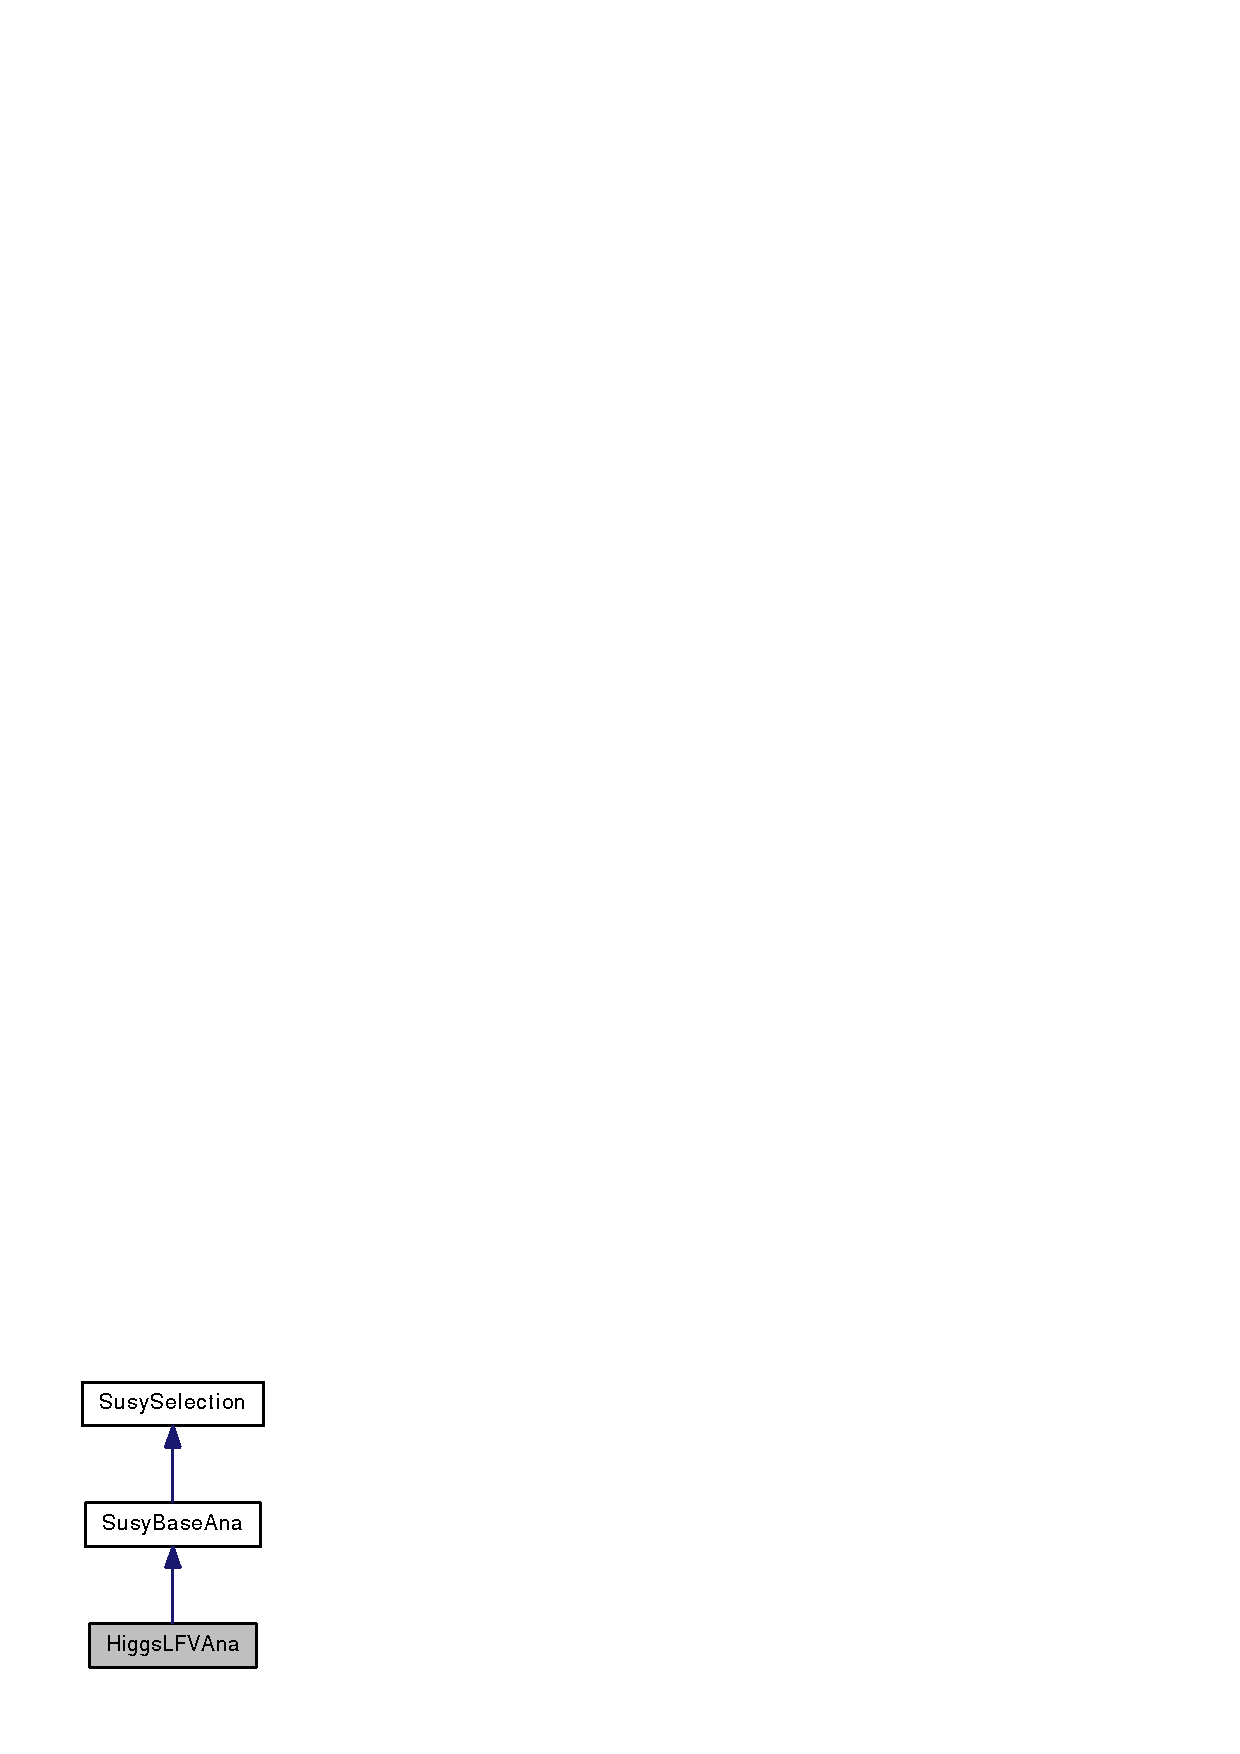
\includegraphics[width=130pt]{classHiggsLFVAna__inherit__graph}
\end{center}
\end{figure}
Collaboration diagram for HiggsLFVAna:\nopagebreak
\begin{figure}[H]
\begin{center}
\leavevmode
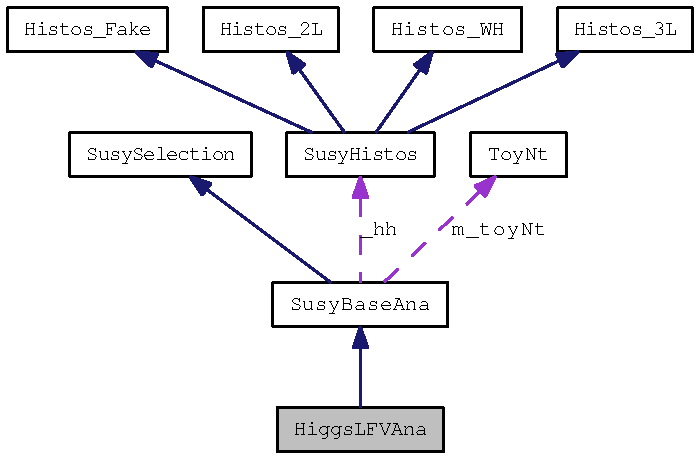
\includegraphics[width=372pt]{classHiggsLFVAna__coll__graph}
\end{center}
\end{figure}
\subsection*{Public Member Functions}
\begin{DoxyCompactItemize}
\item 
\hypertarget{classHiggsLFVAna_a17ede476b7dc2a03c3410c150898c4fa}{
{\bfseries HiggsLFVAna} (\hyperlink{classSusyHistos}{SusyHistos} $\ast$\_\-histos)}
\label{classHiggsLFVAna_a17ede476b7dc2a03c3410c150898c4fa}

\item 
\hypertarget{classHiggsLFVAna_aebdcf3d3fb65aad52279032c6b047e9d}{
void {\bfseries doAnalysis} (float w, unsigned int isys=DGSys\_\-NOM)}
\label{classHiggsLFVAna_aebdcf3d3fb65aad52279032c6b047e9d}

\item 
\hypertarget{classHiggsLFVAna_ab7a299a9b82fa5878efbb6c997d7cc15}{
void {\bfseries end} ()}
\label{classHiggsLFVAna_ab7a299a9b82fa5878efbb6c997d7cc15}

\item 
\hypertarget{classHiggsLFVAna_a590f14d2f9894c48c7f35fcadac67e50}{
void {\bfseries setSelection} (std::string s, uint dilType)}
\label{classHiggsLFVAna_a590f14d2f9894c48c7f35fcadac67e50}

\item 
\hypertarget{classHiggsLFVAna_a641d564bb1c56939b023270f8fdd1c53}{
bool {\bfseries selectEvent} (LeptonVector $\ast$leptons, LeptonVector $\ast$baseLeptons, const JetVector $\ast$jets, const Met $\ast$met, float \_\-ww)}
\label{classHiggsLFVAna_a641d564bb1c56939b023270f8fdd1c53}

\item 
\hypertarget{classHiggsLFVAna_a80a6e0e77dcc10fdce1546b91a4d70a0}{
void {\bfseries fillHistograms} (uint iSR, uint iSYS, const LeptonVector $\ast$leptons, const JetVector $\ast$jets, const Met $\ast$met, float \_\-ww)}
\label{classHiggsLFVAna_a80a6e0e77dcc10fdce1546b91a4d70a0}

\item 
\hypertarget{classHiggsLFVAna_a4677b3064033c4d240ddc4fda48353ec}{
void {\bfseries print\_\-preOS} ()}
\label{classHiggsLFVAna_a4677b3064033c4d240ddc4fda48353ec}

\item 
\hypertarget{classHiggsLFVAna_ad29c474365cdd97419a55e68d9a55ec5}{
{\bfseries ClassDef} (\hyperlink{classHiggsLFVAna}{HiggsLFVAna}, 1)}
\label{classHiggsLFVAna_ad29c474365cdd97419a55e68d9a55ec5}

\end{DoxyCompactItemize}


The documentation for this class was generated from the following files:\begin{DoxyCompactItemize}
\item 
SusyWeakProdAna/HiggsLFVAna.h\item 
Root/HiggsLFVAna.cxx\end{DoxyCompactItemize}

\hypertarget{classHistos__2L}{
\section{Histos\_\-2L Class Reference}
\label{classHistos__2L}\index{Histos\_\-2L@{Histos\_\-2L}}
}
Inheritance diagram for Histos\_\-2L:\nopagebreak
\begin{figure}[H]
\begin{center}
\leavevmode
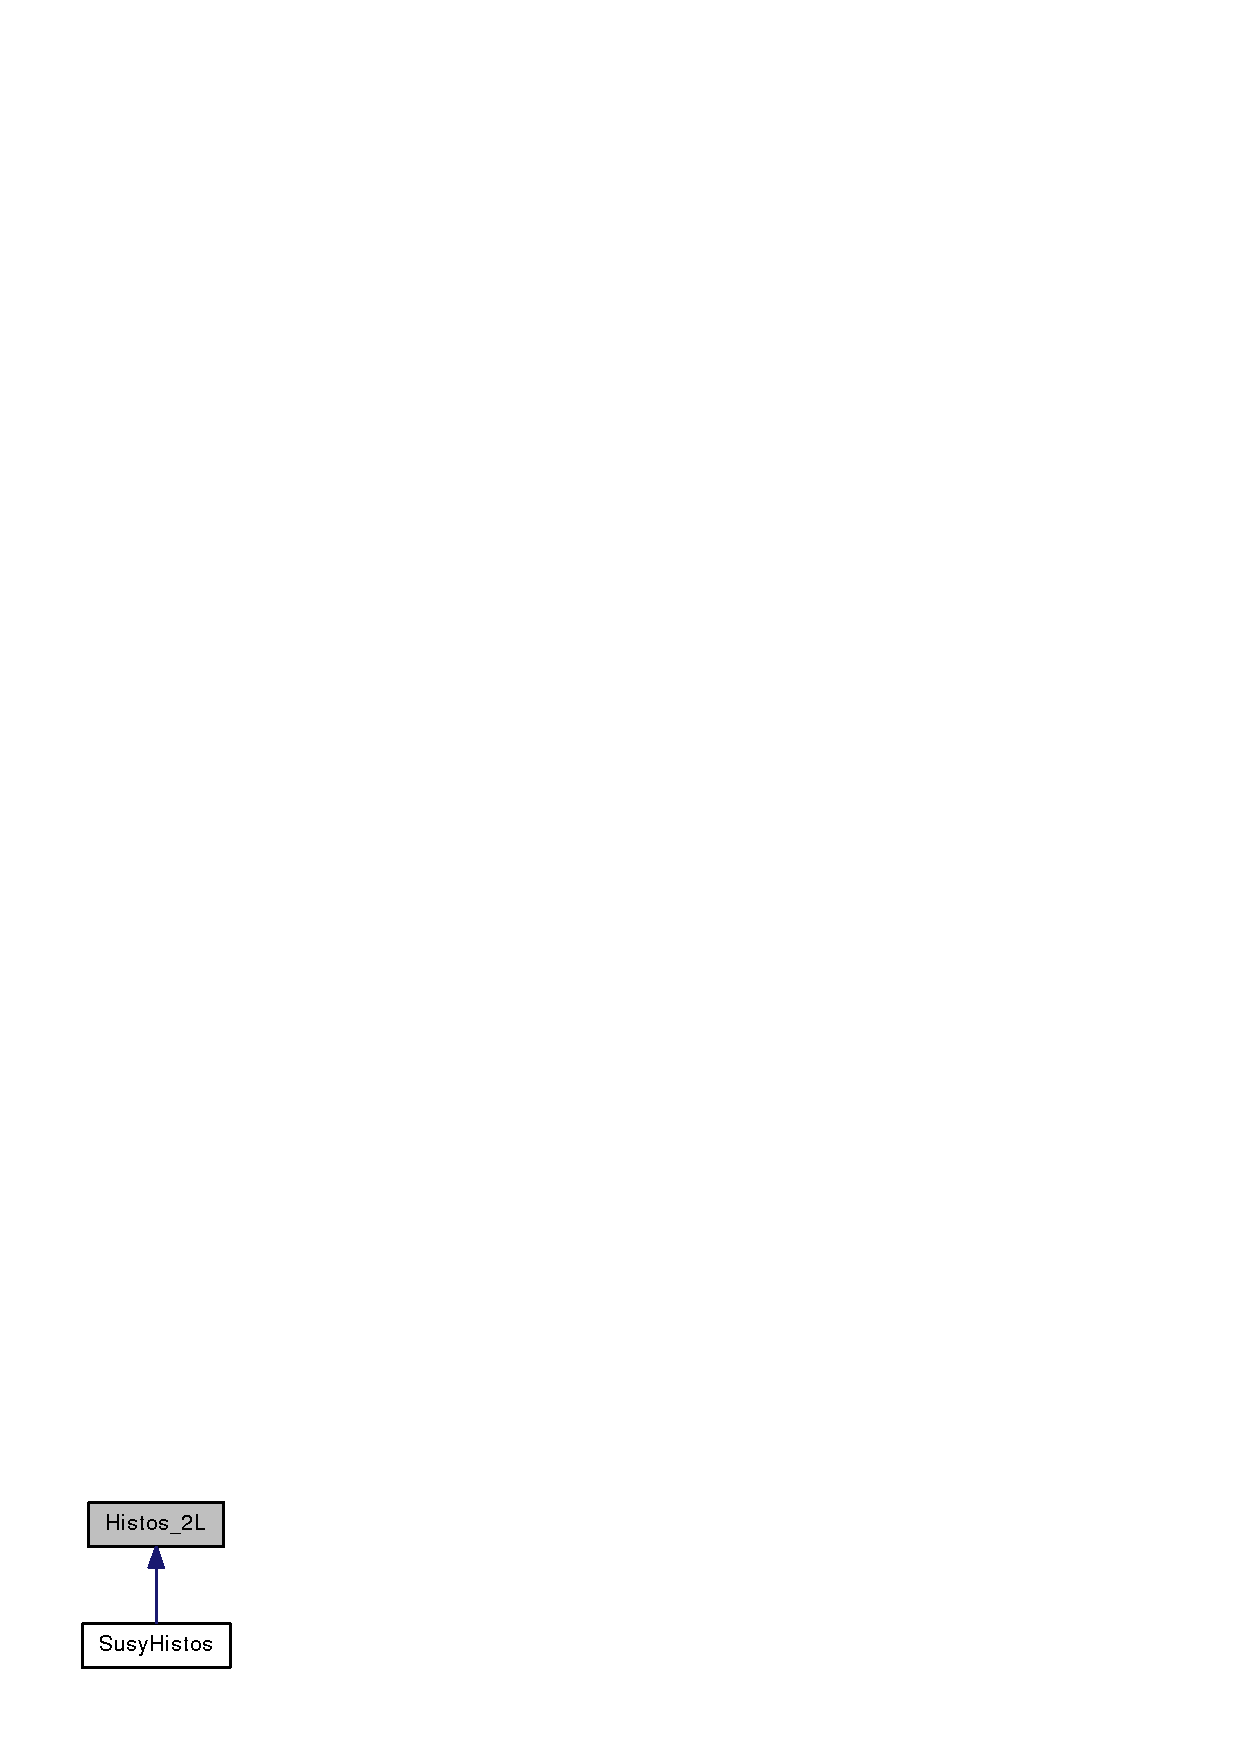
\includegraphics[width=114pt]{classHistos__2L__inherit__graph}
\end{center}
\end{figure}
\subsection*{Public Types}
\begin{DoxyCompactItemize}
\item 
\hypertarget{classHistos__2L_a2c84fab5d2bb387af54bb39f789c2ec8}{
typedef TH1F $\ast$ {\bfseries HDG2L} \mbox{[}DIL\_\-NSR\mbox{]}\mbox{[}3\mbox{]}\mbox{[}DGSys\_\-N\mbox{]}}
\label{classHistos__2L_a2c84fab5d2bb387af54bb39f789c2ec8}

\end{DoxyCompactItemize}
\subsection*{Public Member Functions}
\begin{DoxyCompactItemize}
\item 
\hypertarget{classHistos__2L_ae055a4fb7aed73f03117b50e2093c3c8}{
void {\bfseries Book2LHistograms} (TDirectory $\ast$\_\-hDir, bool useSys=true)}
\label{classHistos__2L_ae055a4fb7aed73f03117b50e2093c3c8}

\item 
\hypertarget{classHistos__2L_a0676e1dd9d70c0b343da9caed055432a}{
{\bfseries ClassDef} (\hyperlink{classHistos__2L}{Histos\_\-2L}, 1)}
\label{classHistos__2L_a0676e1dd9d70c0b343da9caed055432a}

\end{DoxyCompactItemize}
\subsection*{Public Attributes}
\begin{DoxyCompactItemize}
\item 
\hypertarget{classHistos__2L_ac000e2ffb47fabcef580e70dfb2774fb}{
TGuiUtils $\ast$ {\bfseries \_\-utils}}
\label{classHistos__2L_ac000e2ffb47fabcef580e70dfb2774fb}

\item 
\hypertarget{classHistos__2L_aff788383514c40a16d186ba9fe7b634c}{
HDG2L {\bfseries DG2L\_\-pred}}
\label{classHistos__2L_aff788383514c40a16d186ba9fe7b634c}

\item 
\hypertarget{classHistos__2L_ad8193582c03e7175e21ecf31c026897b}{
HDG2L {\bfseries DG2L\_\-Zcount}}
\label{classHistos__2L_ad8193582c03e7175e21ecf31c026897b}

\item 
\hypertarget{classHistos__2L_af72c91320a4b435cd486bbcb62a9154b}{
HDG2L {\bfseries DG2L\_\-cutflow}}
\label{classHistos__2L_af72c91320a4b435cd486bbcb62a9154b}

\item 
\hypertarget{classHistos__2L_a1a659a3b9080df2c45dc3b0832db43b8}{
HDG2L {\bfseries DG2L\_\-nJets}}
\label{classHistos__2L_a1a659a3b9080df2c45dc3b0832db43b8}

\item 
\hypertarget{classHistos__2L_a95d76a3d65fbb2e9e43dac0978d2551f}{
HDG2L {\bfseries DG2L\_\-nCJets}}
\label{classHistos__2L_a95d76a3d65fbb2e9e43dac0978d2551f}

\item 
\hypertarget{classHistos__2L_a74ee8ad0d7b162393d83d858acf34ef7}{
HDG2L {\bfseries DG2L\_\-nFJets}}
\label{classHistos__2L_a74ee8ad0d7b162393d83d858acf34ef7}

\item 
\hypertarget{classHistos__2L_aff092203e83f8bf816155aa10dd0408f}{
HDG2L {\bfseries DG2L\_\-nBJets}}
\label{classHistos__2L_aff092203e83f8bf816155aa10dd0408f}

\item 
\hypertarget{classHistos__2L_a4e931d103726974e80a8727bc895f8a2}{
HDG2L {\bfseries DG2L\_\-nSoftJets}}
\label{classHistos__2L_a4e931d103726974e80a8727bc895f8a2}

\item 
\hypertarget{classHistos__2L_a6cc1fca940ac9bcb1d0268223b004cca}{
HDG2L {\bfseries DG2L\_\-qq}}
\label{classHistos__2L_a6cc1fca940ac9bcb1d0268223b004cca}

\item 
\hypertarget{classHistos__2L_aed50cf7d5f648908e73132834d80a094}{
HDG2L {\bfseries DG2L\_\-mll}}
\label{classHistos__2L_aed50cf7d5f648908e73132834d80a094}

\item 
\hypertarget{classHistos__2L_a777d406ae4700a4a1143e9ac4de504e5}{
HDG2L {\bfseries DG2L\_\-mllcoarse}}
\label{classHistos__2L_a777d406ae4700a4a1143e9ac4de504e5}

\item 
\hypertarget{classHistos__2L_a2f3d6cd1a4af0e1f374096d7f2331020}{
HDG2L {\bfseries DG2L\_\-mllcoarser}}
\label{classHistos__2L_a2f3d6cd1a4af0e1f374096d7f2331020}

\item 
\hypertarget{classHistos__2L_aa38e2199280d7a039991e76d8d7872a4}{
HDG2L {\bfseries DG2L\_\-mjj}}
\label{classHistos__2L_aa38e2199280d7a039991e76d8d7872a4}

\item 
\hypertarget{classHistos__2L_a1f345780bb558ef2617b348e88a232d9}{
HDG2L {\bfseries DG2L\_\-pTll}}
\label{classHistos__2L_a1f345780bb558ef2617b348e88a232d9}

\item 
\hypertarget{classHistos__2L_a567c939119f54dc1681dfdeb837fffa5}{
HDG2L {\bfseries DG2L\_\-mWWT}}
\label{classHistos__2L_a567c939119f54dc1681dfdeb837fffa5}

\item 
\hypertarget{classHistos__2L_ab181aea4efeb6f118866dff1c9a9bf5c}{
HDG2L {\bfseries DG2L\_\-dPhill}}
\label{classHistos__2L_ab181aea4efeb6f118866dff1c9a9bf5c}

\item 
\hypertarget{classHistos__2L_af1ebd6a88063bbf6bab81ca51323784c}{
HDG2L {\bfseries DG2L\_\-dRll}}
\label{classHistos__2L_af1ebd6a88063bbf6bab81ca51323784c}

\item 
\hypertarget{classHistos__2L_a14e77b17bac4fa266a79d5bf7120fb74}{
HDG2L {\bfseries DG2L\_\-dPhilMet}}
\label{classHistos__2L_a14e77b17bac4fa266a79d5bf7120fb74}

\item 
\hypertarget{classHistos__2L_aca9a2d2ef3fd8fa6bf731f2d6b75ab21}{
HDG2L {\bfseries DG2L\_\-dPhiJetMet}}
\label{classHistos__2L_aca9a2d2ef3fd8fa6bf731f2d6b75ab21}

\item 
\hypertarget{classHistos__2L_a3e97a5e1df0c1f26f4a8af06aed711b5}{
HDG2L {\bfseries DG2L\_\-mTl1}}
\label{classHistos__2L_a3e97a5e1df0c1f26f4a8af06aed711b5}

\item 
\hypertarget{classHistos__2L_aad11dc2dc287593f4d5456139b0743c9}{
HDG2L {\bfseries DG2L\_\-mTl2}}
\label{classHistos__2L_aad11dc2dc287593f4d5456139b0743c9}

\item 
\hypertarget{classHistos__2L_a067cecf63171e30df1226e63b1334593}{
HDG2L {\bfseries DG2L\_\-JZBJet}}
\label{classHistos__2L_a067cecf63171e30df1226e63b1334593}

\item 
\hypertarget{classHistos__2L_a90ac3aac527ae85d49ff810a86bc2ed2}{
HDG2L {\bfseries DG2L\_\-JZBEtmiss}}
\label{classHistos__2L_a90ac3aac527ae85d49ff810a86bc2ed2}

\item 
\hypertarget{classHistos__2L_aa41189d2ffed7910d83db946b9a94cc7}{
HDG2L {\bfseries DG2L\_\-etmiss}}
\label{classHistos__2L_aa41189d2ffed7910d83db946b9a94cc7}

\item 
\hypertarget{classHistos__2L_aac810874cb12dc12407d78d6fad6bc4b}{
HDG2L {\bfseries DG2L\_\-etmissPhi}}
\label{classHistos__2L_aac810874cb12dc12407d78d6fad6bc4b}

\item 
\hypertarget{classHistos__2L_abb0a97918c86a16a95c68d25bd0e82ad}{
HDG2L {\bfseries DG2L\_\-metrel}}
\label{classHistos__2L_abb0a97918c86a16a95c68d25bd0e82ad}

\item 
\hypertarget{classHistos__2L_a92042f3a7701cbb920735e0aedae48ef}{
HDG2L {\bfseries DG2L\_\-metrel1}}
\label{classHistos__2L_a92042f3a7701cbb920735e0aedae48ef}

\item 
\hypertarget{classHistos__2L_a8da8e694a0b64e4a745319dd81956c25}{
HDG2L {\bfseries DG2L\_\-metrel2}}
\label{classHistos__2L_a8da8e694a0b64e4a745319dd81956c25}

\item 
\hypertarget{classHistos__2L_a68369ad459c1b1552c4cfd2f3709205e}{
HDG2L {\bfseries DG2L\_\-metrel3}}
\label{classHistos__2L_a68369ad459c1b1552c4cfd2f3709205e}

\item 
\hypertarget{classHistos__2L_a021aab3d9138d601b881466728627049}{
HDG2L {\bfseries DG2L\_\-metRefEle}}
\label{classHistos__2L_a021aab3d9138d601b881466728627049}

\item 
\hypertarget{classHistos__2L_a61fe4ef330ecd8653f33ca488678ab6f}{
HDG2L {\bfseries DG2L\_\-metRefGam}}
\label{classHistos__2L_a61fe4ef330ecd8653f33ca488678ab6f}

\item 
\hypertarget{classHistos__2L_a83d21872a219eac928c76c4fba355240}{
HDG2L {\bfseries DG2L\_\-metRefMuo}}
\label{classHistos__2L_a83d21872a219eac928c76c4fba355240}

\item 
\hypertarget{classHistos__2L_affa8eedd925b981c1f383679e1d89d47}{
HDG2L {\bfseries DG2L\_\-metRefJet}}
\label{classHistos__2L_affa8eedd925b981c1f383679e1d89d47}

\item 
\hypertarget{classHistos__2L_af38a1c885975d20152857e04a2d56b8f}{
HDG2L {\bfseries DG2L\_\-metRefSJet}}
\label{classHistos__2L_af38a1c885975d20152857e04a2d56b8f}

\item 
\hypertarget{classHistos__2L_a84024626aa201465073600d6cfcfeb21}{
HDG2L {\bfseries DG2L\_\-metCellout}}
\label{classHistos__2L_a84024626aa201465073600d6cfcfeb21}

\item 
\hypertarget{classHistos__2L_a02f06dfc25ae8ad51a6300cb11b5354b}{
HDG2L {\bfseries DG2L\_\-mt2}}
\label{classHistos__2L_a02f06dfc25ae8ad51a6300cb11b5354b}

\item 
\hypertarget{classHistos__2L_a1adb01bd59f2abe8defea5765ff26a4d}{
HDG2L {\bfseries DG2L\_\-mt2b}}
\label{classHistos__2L_a1adb01bd59f2abe8defea5765ff26a4d}

\item 
\hypertarget{classHistos__2L_ac196179101012290b7ebd3134364bf09}{
HDG2L {\bfseries DG2L\_\-mct}}
\label{classHistos__2L_ac196179101012290b7ebd3134364bf09}

\item 
\hypertarget{classHistos__2L_a1b6eea51027f1d61c43c326eb33127e1}{
HDG2L {\bfseries DG2L\_\-mctPerp}}
\label{classHistos__2L_a1b6eea51027f1d61c43c326eb33127e1}

\item 
\hypertarget{classHistos__2L_a9816a23078042f259d4e727f68b866d0}{
HDG2L {\bfseries DG2L\_\-mEff}}
\label{classHistos__2L_a9816a23078042f259d4e727f68b866d0}

\item 
\hypertarget{classHistos__2L_a849009ff01446e7ea0e6ec2dd49028b6}{
HDG2L {\bfseries DG2L\_\-mEffwLep}}
\label{classHistos__2L_a849009ff01446e7ea0e6ec2dd49028b6}

\item 
\hypertarget{classHistos__2L_a64b29773720e844bc60d1a09f59adb03}{
HDG2L {\bfseries DG2L\_\-metSig}}
\label{classHistos__2L_a64b29773720e844bc60d1a09f59adb03}

\item 
\hypertarget{classHistos__2L_a2c856f7e932f90dab1a9eefa21687ce4}{
HDG2L {\bfseries DG2L\_\-metSigwLep}}
\label{classHistos__2L_a2c856f7e932f90dab1a9eefa21687ce4}

\item 
\hypertarget{classHistos__2L_a2bd0d39e844a727b207ae9e6fe2d6fd7}{
HDG2L {\bfseries DG2L\_\-ST}}
\label{classHistos__2L_a2bd0d39e844a727b207ae9e6fe2d6fd7}

\item 
\hypertarget{classHistos__2L_ae6002d69f58377010231961621f53f0e}{
HDG2L {\bfseries DG2L\_\-npv}}
\label{classHistos__2L_ae6002d69f58377010231961621f53f0e}

\item 
\hypertarget{classHistos__2L_afb73df47d299a1bd4b0f5f2210643cb7}{
HDG2L {\bfseries DG2L\_\-mu}}
\label{classHistos__2L_afb73df47d299a1bd4b0f5f2210643cb7}

\item 
\hypertarget{classHistos__2L_ae8be7bd4029ebcdafe44669ff68ceba4}{
HDG2L {\bfseries DG2L\_\-ptl1}}
\label{classHistos__2L_ae8be7bd4029ebcdafe44669ff68ceba4}

\item 
\hypertarget{classHistos__2L_a51b35fe226e7a96564b0faf9de6bb47a}{
HDG2L {\bfseries DG2L\_\-ptl2}}
\label{classHistos__2L_a51b35fe226e7a96564b0faf9de6bb47a}

\item 
\hypertarget{classHistos__2L_ab0b12d84972a7b70972baf44cd6475fc}{
HDG2L {\bfseries DG2L\_\-etal1}}
\label{classHistos__2L_ab0b12d84972a7b70972baf44cd6475fc}

\item 
\hypertarget{classHistos__2L_aeb50bb1422b8a43b1b4c572672559ea0}{
HDG2L {\bfseries DG2L\_\-etal2}}
\label{classHistos__2L_aeb50bb1422b8a43b1b4c572672559ea0}

\item 
\hypertarget{classHistos__2L_ac2f4204ff80794a99d4a565de7155b09}{
HDG2L {\bfseries DG2L\_\-ePt}}
\label{classHistos__2L_ac2f4204ff80794a99d4a565de7155b09}

\item 
\hypertarget{classHistos__2L_aef774979887f0273f0360dfdebf5aa11}{
HDG2L {\bfseries DG2L\_\-mPt}}
\label{classHistos__2L_aef774979887f0273f0360dfdebf5aa11}

\item 
\hypertarget{classHistos__2L_aa110adc536a898e8ff2ffa5598ed9a25}{
HDG2L {\bfseries DG2L\_\-eEta}}
\label{classHistos__2L_aa110adc536a898e8ff2ffa5598ed9a25}

\item 
\hypertarget{classHistos__2L_a516727af813b86607319ed47e82463d0}{
HDG2L {\bfseries DG2L\_\-mEta}}
\label{classHistos__2L_a516727af813b86607319ed47e82463d0}

\item 
\hypertarget{classHistos__2L_acafb0ed0ff7100af928fed4bde7a0f2d}{
HDG2L {\bfseries DG2L\_\-d0Sl1}}
\label{classHistos__2L_acafb0ed0ff7100af928fed4bde7a0f2d}

\item 
\hypertarget{classHistos__2L_acf6f5d5dacf6468d2d3b31737f1a7df2}{
HDG2L {\bfseries DG2L\_\-d0Sl2}}
\label{classHistos__2L_acf6f5d5dacf6468d2d3b31737f1a7df2}

\item 
\hypertarget{classHistos__2L_a96a4653adf0032f3d85961ec0eefe0d7}{
HDG2L {\bfseries DG2L\_\-z0sinthetal1}}
\label{classHistos__2L_a96a4653adf0032f3d85961ec0eefe0d7}

\item 
\hypertarget{classHistos__2L_a2387273dd4f1d0ac513ba04481cf572c}{
HDG2L {\bfseries DG2L\_\-z0sinthetal2}}
\label{classHistos__2L_a2387273dd4f1d0ac513ba04481cf572c}

\item 
\hypertarget{classHistos__2L_a2ffa7fcaf30bbca5b4fc22c0743e36c7}{
HDG2L {\bfseries DG2L\_\-orgl1}}
\label{classHistos__2L_a2ffa7fcaf30bbca5b4fc22c0743e36c7}

\item 
\hypertarget{classHistos__2L_a3dfc734e6f406eae6b688a476bd9d136}{
HDG2L {\bfseries DG2L\_\-orgl2}}
\label{classHistos__2L_a3dfc734e6f406eae6b688a476bd9d136}

\item 
\hypertarget{classHistos__2L_a880202b484802ce05dd4035a90b1763c}{
HDG2L {\bfseries DG2L\_\-ptj1}}
\label{classHistos__2L_a880202b484802ce05dd4035a90b1763c}

\item 
\hypertarget{classHistos__2L_a135870f122b54f071b17cad26483a683}{
HDG2L {\bfseries DG2L\_\-ptj2}}
\label{classHistos__2L_a135870f122b54f071b17cad26483a683}

\item 
\hypertarget{classHistos__2L_a2a3938c62856bc92164635a0c4b7bbf2}{
HDG2L {\bfseries DG2L\_\-ptj3}}
\label{classHistos__2L_a2a3938c62856bc92164635a0c4b7bbf2}

\item 
\hypertarget{classHistos__2L_a7966870e01e3a29443d840feb5a030aa}{
HDG2L {\bfseries DG2L\_\-ptj4}}
\label{classHistos__2L_a7966870e01e3a29443d840feb5a030aa}

\item 
\hypertarget{classHistos__2L_adfd30491f35725212379b32841e531a1}{
HDG2L {\bfseries DG2L\_\-etaj1}}
\label{classHistos__2L_adfd30491f35725212379b32841e531a1}

\item 
\hypertarget{classHistos__2L_a595deefdbd84116bb6776b3613c07c6d}{
HDG2L {\bfseries DG2L\_\-etaj2}}
\label{classHistos__2L_a595deefdbd84116bb6776b3613c07c6d}

\item 
\hypertarget{classHistos__2L_a7ca45ebd7be765acad4ee25db9b16506}{
HDG2L {\bfseries DG2L\_\-etaj3}}
\label{classHistos__2L_a7ca45ebd7be765acad4ee25db9b16506}

\item 
\hypertarget{classHistos__2L_a3f8355f535a39e13874d33886228f3dc}{
HDG2L {\bfseries DG2L\_\-etaj4}}
\label{classHistos__2L_a3f8355f535a39e13874d33886228f3dc}

\item 
\hypertarget{classHistos__2L_a4840cb98ce1d0b7485ce7fa4bb89c1e5}{
HDG2L {\bfseries DG2L\_\-jvfj1}}
\label{classHistos__2L_a4840cb98ce1d0b7485ce7fa4bb89c1e5}

\item 
\hypertarget{classHistos__2L_add7d49af1fd579d576d8b724ed25a596}{
HDG2L {\bfseries DG2L\_\-jvfj2}}
\label{classHistos__2L_add7d49af1fd579d576d8b724ed25a596}

\item 
\hypertarget{classHistos__2L_a039246b73256c9f6406874a8d94d1f26}{
HDG2L {\bfseries DG2L\_\-ptbj}}
\label{classHistos__2L_a039246b73256c9f6406874a8d94d1f26}

\item 
\hypertarget{classHistos__2L_abc2dc6d922722179b6c4f82f789658c8}{
HDG2L {\bfseries DG2L\_\-etabj}}
\label{classHistos__2L_abc2dc6d922722179b6c4f82f789658c8}

\item 
\hypertarget{classHistos__2L_abe39d015a70037bc57338fbcd43d830b}{
HDG2L {\bfseries DG2L\_\-jvfbj}}
\label{classHistos__2L_abe39d015a70037bc57338fbcd43d830b}

\item 
\hypertarget{classHistos__2L_a2cd995114bda7bd39f5b55b0b1ab4ed5}{
HDG2L {\bfseries DG2L\_\-ptSj1}}
\label{classHistos__2L_a2cd995114bda7bd39f5b55b0b1ab4ed5}

\item 
\hypertarget{classHistos__2L_ab112edab267a8bbe28fd9d7e280e6f5e}{
HDG2L {\bfseries DG2L\_\-ptSj2}}
\label{classHistos__2L_ab112edab267a8bbe28fd9d7e280e6f5e}

\item 
\hypertarget{classHistos__2L_ab04be18de61abbcb5a5368342b02235e}{
HDG2L {\bfseries DG2L\_\-etaSj1}}
\label{classHistos__2L_ab04be18de61abbcb5a5368342b02235e}

\item 
\hypertarget{classHistos__2L_a9bb6f023aa09a9252ae2f4d6acc76082}{
HDG2L {\bfseries DG2L\_\-etaSj2}}
\label{classHistos__2L_a9bb6f023aa09a9252ae2f4d6acc76082}

\item 
\hypertarget{classHistos__2L_ab3182ec8c35d102e46105d077ee58020}{
HDG2L {\bfseries DG2L\_\-jvfSj1}}
\label{classHistos__2L_ab3182ec8c35d102e46105d077ee58020}

\item 
\hypertarget{classHistos__2L_a29edb97b293229d8b74f89e076f6b7d1}{
HDG2L {\bfseries DG2L\_\-jvfSj2}}
\label{classHistos__2L_a29edb97b293229d8b74f89e076f6b7d1}

\item 
\hypertarget{classHistos__2L_a9c1b9eac02370718702a0519ae92fef4}{
std::map$<$ int, int $>$ {\bfseries runBins}}
\label{classHistos__2L_a9c1b9eac02370718702a0519ae92fef4}

\end{DoxyCompactItemize}


The documentation for this class was generated from the following files:\begin{DoxyCompactItemize}
\item 
SusyWeakProdAna/Histos\_\-2L.h\item 
Root/Histos\_\-2L.cxx\end{DoxyCompactItemize}

\hypertarget{classHistos__3L}{
\section{Histos\_\-3L Class Reference}
\label{classHistos__3L}\index{Histos\_\-3L@{Histos\_\-3L}}
}
Inheritance diagram for Histos\_\-3L:\nopagebreak
\begin{figure}[H]
\begin{center}
\leavevmode
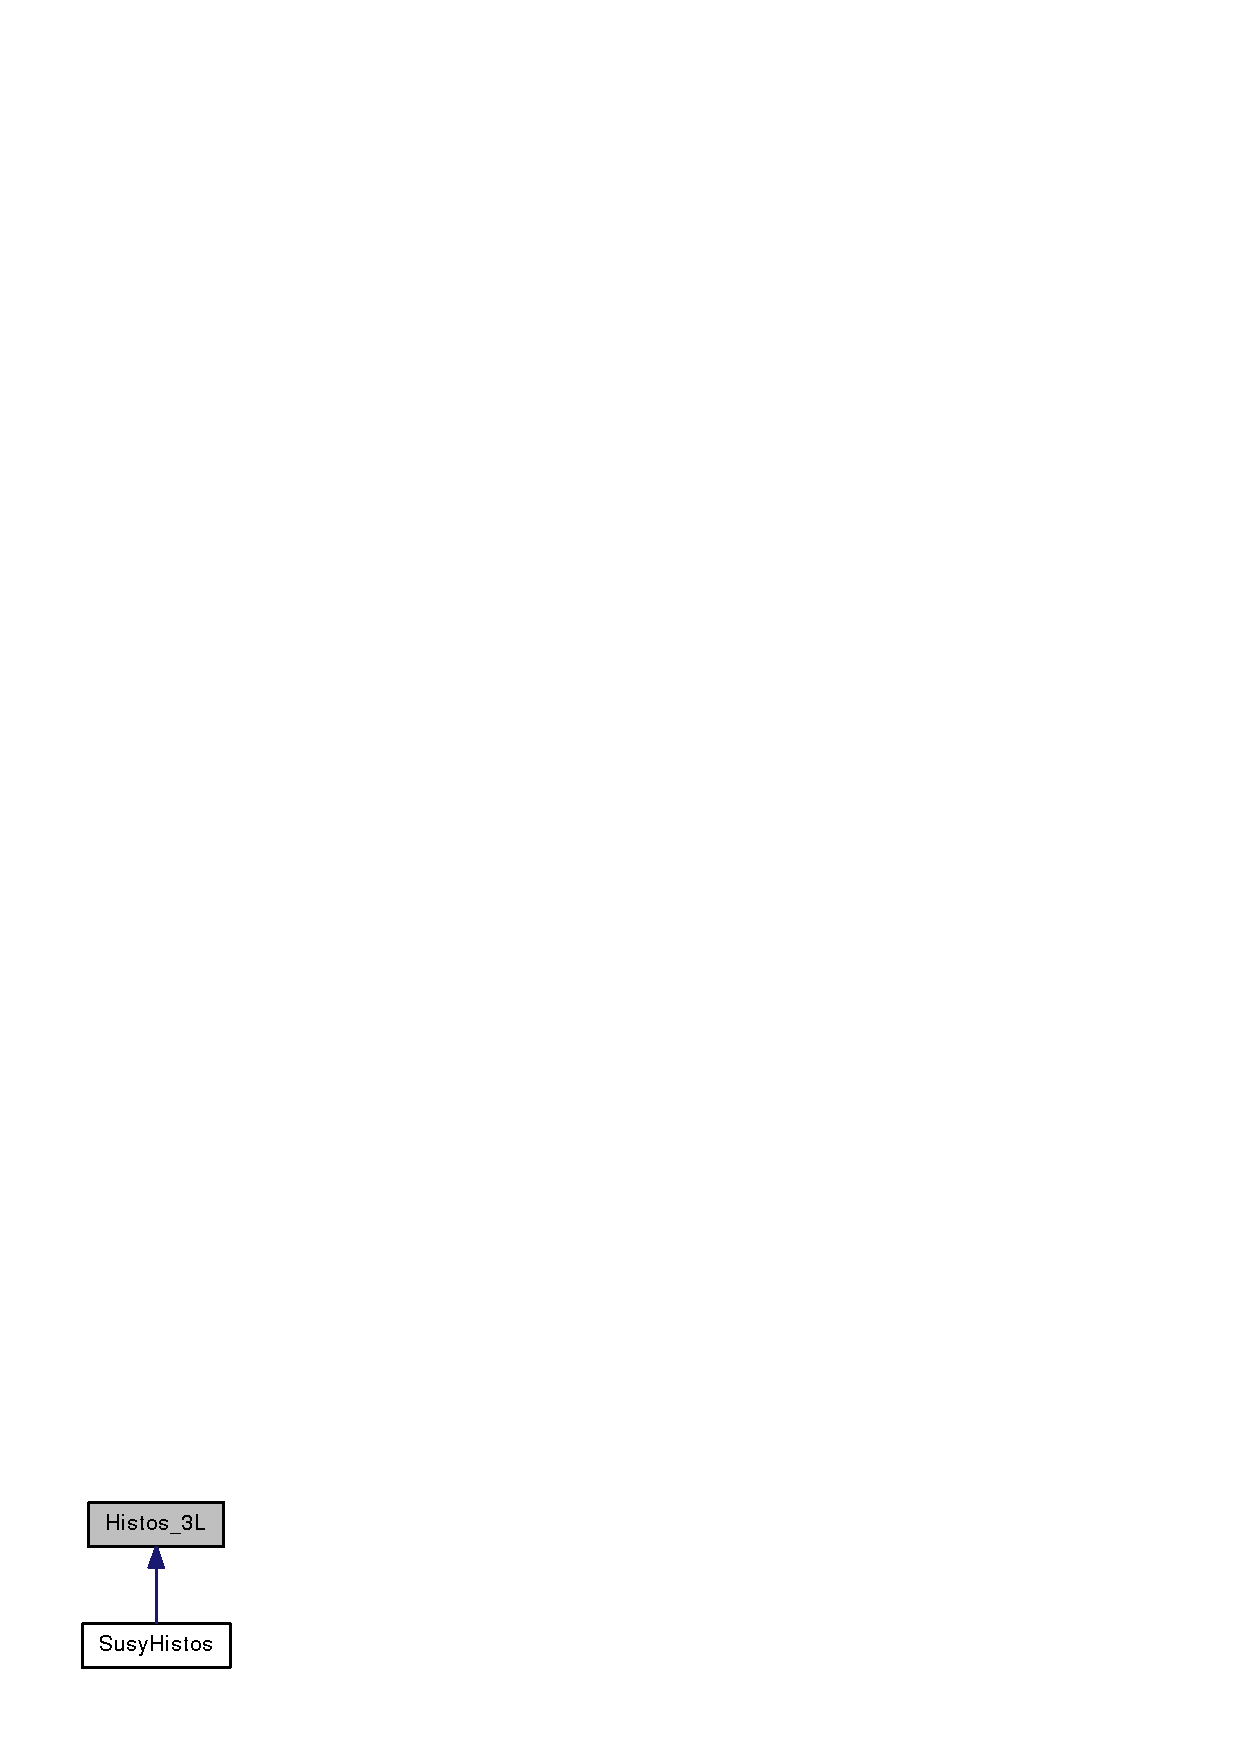
\includegraphics[width=114pt]{classHistos__3L__inherit__graph}
\end{center}
\end{figure}
\subsection*{Public Types}
\begin{DoxyCompactItemize}
\item 
\hypertarget{classHistos__3L_a952977bc68eea6cfd22880aa36068a45}{
typedef TH1F $\ast$ {\bfseries HML} \mbox{[}ML\_\-NSR\mbox{]}\mbox{[}ML\_\-N\mbox{]}\mbox{[}DGSys\_\-N\mbox{]}}
\label{classHistos__3L_a952977bc68eea6cfd22880aa36068a45}

\end{DoxyCompactItemize}
\subsection*{Public Member Functions}
\begin{DoxyCompactItemize}
\item 
\hypertarget{classHistos__3L_a3831a414422d4088e11530d7719fe71e}{
void {\bfseries Book3LHistograms} (TDirectory $\ast$\_\-hDir, bool useSys=true)}
\label{classHistos__3L_a3831a414422d4088e11530d7719fe71e}

\item 
\hypertarget{classHistos__3L_a759eec3fd0f1d2d70473284fa8b3a4da}{
void {\bfseries Sum3LHistograms} ()}
\label{classHistos__3L_a759eec3fd0f1d2d70473284fa8b3a4da}

\item 
\hyperlink{classHistos__3L_a7d0bc7498db9a0508da4d58188746ae0}{ClassDef} (\hyperlink{classHistos__3L}{Histos\_\-3L}, 1)
\end{DoxyCompactItemize}
\subsection*{Public Attributes}
\begin{DoxyCompactItemize}
\item 
\hypertarget{classHistos__3L_ad7050c3b0809b89afe3e33a7bdf00edc}{
TGuiUtils $\ast$ {\bfseries \_\-utils}}
\label{classHistos__3L_ad7050c3b0809b89afe3e33a7bdf00edc}

\item 
\hypertarget{classHistos__3L_aa353fd3a5a0fd545fd6a1df989e69395}{
HML {\bfseries ML\_\-pred}}
\label{classHistos__3L_aa353fd3a5a0fd545fd6a1df989e69395}

\item 
\hypertarget{classHistos__3L_ad6f450fd20e5241c55d391c7ea096aa3}{
HML {\bfseries ML\_\-predGe2J}}
\label{classHistos__3L_ad6f450fd20e5241c55d391c7ea096aa3}

\item 
\hypertarget{classHistos__3L_a29cb06fa81c126a7faf5b587e5bcfcb2}{
HML {\bfseries ML\_\-cutflow}}
\label{classHistos__3L_a29cb06fa81c126a7faf5b587e5bcfcb2}

\item 
\hypertarget{classHistos__3L_a2a8d17cb50411b12118750df2ca9fc00}{
HML {\bfseries ML\_\-evtCatgUnOrdered}}
\label{classHistos__3L_a2a8d17cb50411b12118750df2ca9fc00}

\item 
\hypertarget{classHistos__3L_a381528cba82f33fa55c0d74c6b571927}{
HML {\bfseries ML\_\-evtCatgOSpair}}
\label{classHistos__3L_a381528cba82f33fa55c0d74c6b571927}

\item 
\hypertarget{classHistos__3L_a9d795c3fc2969461b646a6b48fe702aa}{
HML {\bfseries ML\_\-evtCatgSSpair}}
\label{classHistos__3L_a9d795c3fc2969461b646a6b48fe702aa}

\item 
\hypertarget{classHistos__3L_ab3c2f420c7c9a7ecb93047c4203f9b1c}{
HML {\bfseries ML\_\-nLep}}
\label{classHistos__3L_ab3c2f420c7c9a7ecb93047c4203f9b1c}

\item 
\hypertarget{classHistos__3L_a04b24da0f47cd7698109fc9eaefd09ee}{
HML {\bfseries ML\_\-nJets}}
\label{classHistos__3L_a04b24da0f47cd7698109fc9eaefd09ee}

\item 
\hypertarget{classHistos__3L_acd5004bb35c70862327d8e0bb9f5b610}{
HML {\bfseries ML\_\-nBJets}}
\label{classHistos__3L_acd5004bb35c70862327d8e0bb9f5b610}

\item 
\hypertarget{classHistos__3L_a195e59c7bfef0fe97e71be5190d47216}{
HML {\bfseries ML\_\-SFOSMll}}
\label{classHistos__3L_a195e59c7bfef0fe97e71be5190d47216}

\item 
\hypertarget{classHistos__3L_a4827b3f6220a2d150764ba185e066045}{
HML {\bfseries ML\_\-SFOSMlll}}
\label{classHistos__3L_a4827b3f6220a2d150764ba185e066045}

\item 
\hypertarget{classHistos__3L_a5ced4544cd9a321ce4ee59a0338502f6}{
HML {\bfseries ML\_\-AllMll}}
\label{classHistos__3L_a5ced4544cd9a321ce4ee59a0338502f6}

\item 
\hypertarget{classHistos__3L_a75a903963111c6c3ab97b3ee2c13141d}{
HML {\bfseries ML\_\-AllMlll}}
\label{classHistos__3L_a75a903963111c6c3ab97b3ee2c13141d}

\item 
\hypertarget{classHistos__3L_a9b68ae5f97d853f0892cfe68f23f5750}{
HML {\bfseries ML\_\-SFOSMZZ}}
\label{classHistos__3L_a9b68ae5f97d853f0892cfe68f23f5750}

\item 
\hypertarget{classHistos__3L_a86f600399896f255416bb49f53983628}{
HML {\bfseries ML\_\-SFOSMT}}
\label{classHistos__3L_a86f600399896f255416bb49f53983628}

\item 
\hypertarget{classHistos__3L_ab3b24b0e4bcfd746cbfd8ccb5adb60d9}{
HML {\bfseries ML\_\-mct}}
\label{classHistos__3L_ab3b24b0e4bcfd746cbfd8ccb5adb60d9}

\item 
\hypertarget{classHistos__3L_a65021e382e68da2399cf77bc0d338b41}{
HML {\bfseries ML\_\-mctPerp}}
\label{classHistos__3L_a65021e382e68da2399cf77bc0d338b41}

\item 
\hypertarget{classHistos__3L_a5184575f186e2c7462d19d4f7ab4d57e}{
HML {\bfseries ML\_\-mt2}}
\label{classHistos__3L_a5184575f186e2c7462d19d4f7ab4d57e}

\item 
\hypertarget{classHistos__3L_a55005854fcf337da9dcd4e18cc0851b1}{
HML {\bfseries ML\_\-mt2b}}
\label{classHistos__3L_a55005854fcf337da9dcd4e18cc0851b1}

\item 
\hypertarget{classHistos__3L_a7ac79733eef8ff630a051c667b5c7f1a}{
HML {\bfseries ML\_\-mct\_\-0J}}
\label{classHistos__3L_a7ac79733eef8ff630a051c667b5c7f1a}

\item 
\hypertarget{classHistos__3L_a617d91bc4b7372eb5899a018f69d8289}{
HML {\bfseries ML\_\-mctPerp\_\-0J}}
\label{classHistos__3L_a617d91bc4b7372eb5899a018f69d8289}

\item 
\hypertarget{classHistos__3L_a92bd434f7515c15bcaf4b5c3944cd77f}{
HML {\bfseries ML\_\-mt2\_\-0J}}
\label{classHistos__3L_a92bd434f7515c15bcaf4b5c3944cd77f}

\item 
\hypertarget{classHistos__3L_a8d1705be448e5db76d254699948278c6}{
HML {\bfseries ML\_\-mt2b\_\-0J}}
\label{classHistos__3L_a8d1705be448e5db76d254699948278c6}

\item 
\hypertarget{classHistos__3L_a07610729a035c56ebd82649ed43e5888}{
HML {\bfseries ML\_\-etmiss}}
\label{classHistos__3L_a07610729a035c56ebd82649ed43e5888}

\item 
\hypertarget{classHistos__3L_ad02a9fc9b371daa96be3207d5a85b92a}{
HML {\bfseries ML\_\-metrel}}
\label{classHistos__3L_ad02a9fc9b371daa96be3207d5a85b92a}

\item 
\hypertarget{classHistos__3L_afe0164b051bc3cd27f993980421f7545}{
HML {\bfseries ML\_\-meff}}
\label{classHistos__3L_afe0164b051bc3cd27f993980421f7545}

\item 
\hypertarget{classHistos__3L_ae528eec6c4f5870a92f3a22fb0a24be5}{
HML {\bfseries ML\_\-metSig}}
\label{classHistos__3L_ae528eec6c4f5870a92f3a22fb0a24be5}

\item 
\hypertarget{classHistos__3L_ae261f9c0b1dc234f6ab4ea079013f59f}{
HML {\bfseries ML\_\-metRefEle}}
\label{classHistos__3L_ae261f9c0b1dc234f6ab4ea079013f59f}

\item 
\hypertarget{classHistos__3L_adb9ba310647211c1e5cfad6bc94a6641}{
HML {\bfseries ML\_\-metRefGam}}
\label{classHistos__3L_adb9ba310647211c1e5cfad6bc94a6641}

\item 
\hypertarget{classHistos__3L_af607ead64616328a0fc2a9adb6aef099}{
HML {\bfseries ML\_\-metRefMuo}}
\label{classHistos__3L_af607ead64616328a0fc2a9adb6aef099}

\item 
\hypertarget{classHistos__3L_a22870cfa448613af5dbb588677f9b340}{
HML {\bfseries ML\_\-metRefJet}}
\label{classHistos__3L_a22870cfa448613af5dbb588677f9b340}

\item 
\hypertarget{classHistos__3L_a1e9c207d39020158123cbeba559c970b}{
HML {\bfseries ML\_\-metRefSJet}}
\label{classHistos__3L_a1e9c207d39020158123cbeba559c970b}

\item 
\hypertarget{classHistos__3L_ac84ba3456fe0d46585f8fdd4121307a8}{
HML {\bfseries ML\_\-metCellout}}
\label{classHistos__3L_ac84ba3456fe0d46585f8fdd4121307a8}

\item 
\hypertarget{classHistos__3L_a24883d08bd8f134b8591e6db5e4317eb}{
HML {\bfseries ML\_\-ptl1}}
\label{classHistos__3L_a24883d08bd8f134b8591e6db5e4317eb}

\item 
\hypertarget{classHistos__3L_a19feb0b069a1d63a3bd9e5000f378a18}{
HML {\bfseries ML\_\-ptl2}}
\label{classHistos__3L_a19feb0b069a1d63a3bd9e5000f378a18}

\item 
\hypertarget{classHistos__3L_ab4146bcfc0350cef01c391ab655d8556}{
HML {\bfseries ML\_\-ptl3}}
\label{classHistos__3L_ab4146bcfc0350cef01c391ab655d8556}

\item 
\hypertarget{classHistos__3L_a33420be76e840f237501c0e26ca6d4ae}{
HML {\bfseries ML\_\-ptl4}}
\label{classHistos__3L_a33420be76e840f237501c0e26ca6d4ae}

\item 
\hypertarget{classHistos__3L_ae2f7a1c9a4f389989dcadc8c12cad69e}{
HML {\bfseries ML\_\-etal1}}
\label{classHistos__3L_ae2f7a1c9a4f389989dcadc8c12cad69e}

\item 
\hypertarget{classHistos__3L_ad9bae9b30718377035310733df9c9200}{
HML {\bfseries ML\_\-etal2}}
\label{classHistos__3L_ad9bae9b30718377035310733df9c9200}

\item 
\hypertarget{classHistos__3L_adeb5201e74a976ac4f80c765498aed68}{
HML {\bfseries ML\_\-etal3}}
\label{classHistos__3L_adeb5201e74a976ac4f80c765498aed68}

\item 
\hypertarget{classHistos__3L_a7f62833c8b934057aa58c0e5353ce525}{
HML {\bfseries ML\_\-etal4}}
\label{classHistos__3L_a7f62833c8b934057aa58c0e5353ce525}

\item 
\hypertarget{classHistos__3L_acf677e41bb756d564f1629a5b2cb56b8}{
HML {\bfseries ML\_\-d0Sl1}}
\label{classHistos__3L_acf677e41bb756d564f1629a5b2cb56b8}

\item 
\hypertarget{classHistos__3L_a92f2f0b297ac8672a8bd65a6050585df}{
HML {\bfseries ML\_\-d0Sl2}}
\label{classHistos__3L_a92f2f0b297ac8672a8bd65a6050585df}

\item 
\hypertarget{classHistos__3L_a5b509b43185582271ea08d738a43cd7a}{
HML {\bfseries ML\_\-d0Sl3}}
\label{classHistos__3L_a5b509b43185582271ea08d738a43cd7a}

\item 
\hypertarget{classHistos__3L_acbff9ded0b3b5c7758d1d4e9980652e3}{
HML {\bfseries ML\_\-d0Sl4}}
\label{classHistos__3L_acbff9ded0b3b5c7758d1d4e9980652e3}

\item 
\hypertarget{classHistos__3L_aa46b48873521ebecbd2545561cf21b89}{
HML {\bfseries ML\_\-z0sinthetal1}}
\label{classHistos__3L_aa46b48873521ebecbd2545561cf21b89}

\item 
\hypertarget{classHistos__3L_a0d3a43e17886cfb61a7b8505102221dd}{
HML {\bfseries ML\_\-z0sinthetal2}}
\label{classHistos__3L_a0d3a43e17886cfb61a7b8505102221dd}

\item 
\hypertarget{classHistos__3L_ad9a3694d1b6187b4ad30bde614b06c1c}{
HML {\bfseries ML\_\-z0sinthetal3}}
\label{classHistos__3L_ad9a3694d1b6187b4ad30bde614b06c1c}

\item 
\hypertarget{classHistos__3L_a0a7f1bf61a3c3c8acfa681f6de715ab0}{
HML {\bfseries ML\_\-z0sinthetal4}}
\label{classHistos__3L_a0a7f1bf61a3c3c8acfa681f6de715ab0}

\item 
\hypertarget{classHistos__3L_abba487eabd50180e4a4d1b04563d3c33}{
HML {\bfseries ML\_\-orgl1}}
\label{classHistos__3L_abba487eabd50180e4a4d1b04563d3c33}

\item 
\hypertarget{classHistos__3L_a3278a0d64d1bf7003ee86c046bbb9251}{
HML {\bfseries ML\_\-orgl2}}
\label{classHistos__3L_a3278a0d64d1bf7003ee86c046bbb9251}

\item 
\hypertarget{classHistos__3L_a94beadaf6b60059b510379f78428e444}{
HML {\bfseries ML\_\-orgl3}}
\label{classHistos__3L_a94beadaf6b60059b510379f78428e444}

\item 
\hypertarget{classHistos__3L_a38c4b12657b79908d453cbc6b54b4afc}{
HML {\bfseries ML\_\-orgl4}}
\label{classHistos__3L_a38c4b12657b79908d453cbc6b54b4afc}

\item 
\hypertarget{classHistos__3L_a72859e81c38a02fd4ad6d0d45e10d5c4}{
HML {\bfseries ML\_\-pTll}}
\label{classHistos__3L_a72859e81c38a02fd4ad6d0d45e10d5c4}

\item 
\hypertarget{classHistos__3L_a8bdbfc98d5a60f5ac0034c01ac244c48}{
HML {\bfseries ML\_\-dRll}}
\label{classHistos__3L_a8bdbfc98d5a60f5ac0034c01ac244c48}

\item 
\hypertarget{classHistos__3L_a15a632f5ecae14f9a70964a1a1c5ec8d}{
HML {\bfseries ML\_\-ptj1}}
\label{classHistos__3L_a15a632f5ecae14f9a70964a1a1c5ec8d}

\item 
\hypertarget{classHistos__3L_a8b65e14b0c1a295da03925b1dcb112a0}{
HML {\bfseries ML\_\-ptj2}}
\label{classHistos__3L_a8b65e14b0c1a295da03925b1dcb112a0}

\item 
\hypertarget{classHistos__3L_a928c4a359c04c8152cc9f4b05be8bfea}{
HML {\bfseries ML\_\-ptj3}}
\label{classHistos__3L_a928c4a359c04c8152cc9f4b05be8bfea}

\item 
\hypertarget{classHistos__3L_a93f4c4a27d2680719e0d052729d057e0}{
HML {\bfseries ML\_\-ptj4}}
\label{classHistos__3L_a93f4c4a27d2680719e0d052729d057e0}

\item 
\hypertarget{classHistos__3L_a8d07d814793cc423c43124f8df619585}{
HML {\bfseries ML\_\-mjj}}
\label{classHistos__3L_a8d07d814793cc423c43124f8df619585}

\item 
\hypertarget{classHistos__3L_afba4ba8d85675a13697feb33f28c6785}{
HML {\bfseries ML\_\-etaj1}}
\label{classHistos__3L_afba4ba8d85675a13697feb33f28c6785}

\item 
\hypertarget{classHistos__3L_a61f02b72fb3a0795bdb168f24f2de50c}{
HML {\bfseries ML\_\-etaj2}}
\label{classHistos__3L_a61f02b72fb3a0795bdb168f24f2de50c}

\item 
\hypertarget{classHistos__3L_ad916eef6b3683d9fb39fdb33d71a493f}{
HML {\bfseries ML\_\-etaj3}}
\label{classHistos__3L_ad916eef6b3683d9fb39fdb33d71a493f}

\item 
\hypertarget{classHistos__3L_a9e1261f97b007a261ad890a9138d18f1}{
HML {\bfseries ML\_\-etaj4}}
\label{classHistos__3L_a9e1261f97b007a261ad890a9138d18f1}

\item 
\hypertarget{classHistos__3L_a5c8aaeaf11a608d10ee96bbe1ce5b32b}{
HML {\bfseries ML\_\-ptbj}}
\label{classHistos__3L_a5c8aaeaf11a608d10ee96bbe1ce5b32b}

\item 
\hypertarget{classHistos__3L_aaab38749a5ca33bdd72bbd1d565338b0}{
HML {\bfseries ML\_\-etabj}}
\label{classHistos__3L_aaab38749a5ca33bdd72bbd1d565338b0}

\end{DoxyCompactItemize}


\subsection{Member Function Documentation}
\hypertarget{classHistos__3L_a7d0bc7498db9a0508da4d58188746ae0}{
\index{Histos\_\-3L@{Histos\_\-3L}!ClassDef@{ClassDef}}
\index{ClassDef@{ClassDef}!Histos_3L@{Histos\_\-3L}}
\subsubsection[{ClassDef}]{\setlength{\rightskip}{0pt plus 5cm}Histos\_\-3L::ClassDef ({\bf Histos\_\-3L}, \/  1)}}
\label{classHistos__3L_a7d0bc7498db9a0508da4d58188746ae0}
Fill histo given SR for ML 

The documentation for this class was generated from the following files:\begin{DoxyCompactItemize}
\item 
SusyWeakProdAna/Histos\_\-3L.h\item 
Root/Histos\_\-3L.cxx\end{DoxyCompactItemize}

\hypertarget{classHistos__Fake}{
\section{Histos\_\-Fake Class Reference}
\label{classHistos__Fake}\index{Histos\_\-Fake@{Histos\_\-Fake}}
}
Inheritance diagram for Histos\_\-Fake:\nopagebreak
\begin{figure}[H]
\begin{center}
\leavevmode
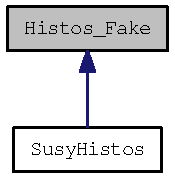
\includegraphics[width=120pt]{classHistos__Fake__inherit__graph}
\end{center}
\end{figure}
\subsection*{Public Member Functions}
\begin{DoxyCompactItemize}
\item 
\hypertarget{classHistos__Fake_a0656561e3aaeed2986075f8b3935e084}{
void {\bfseries BookFakeHistograms} (TDirectory $\ast$\_\-hDir)}
\label{classHistos__Fake_a0656561e3aaeed2986075f8b3935e084}

\item 
\hypertarget{classHistos__Fake_a757e776a903c6f4f8472194682d4f3a5}{
TH1F $\ast$ {\bfseries DEF\_\-HPROBE} (m\_\-org)}
\label{classHistos__Fake_a757e776a903c6f4f8472194682d4f3a5}

\item 
\hypertarget{classHistos__Fake_ad12ead3103dfccbdcc3838665c54b314}{
TH1F $\ast$ {\bfseries DEF\_\-HPROBE} (m\_\-type)}
\label{classHistos__Fake_ad12ead3103dfccbdcc3838665c54b314}

\item 
\hypertarget{classHistos__Fake_a083980196a559361d9acda477775e568}{
TH1F $\ast$ {\bfseries DEF\_\-HPROBE} (m\_\-pt)}
\label{classHistos__Fake_a083980196a559361d9acda477775e568}

\item 
\hypertarget{classHistos__Fake_a82f441751f9ecc434ec43e23e6883385}{
TH1F $\ast$ {\bfseries DEF\_\-HPROBE} (m\_\-eta)}
\label{classHistos__Fake_a82f441751f9ecc434ec43e23e6883385}

\item 
\hypertarget{classHistos__Fake_ac5618093543addbb07899bff6ee11803}{
TH1F $\ast$ {\bfseries DEF\_\-HPROBE} (m\_\-d0)}
\label{classHistos__Fake_ac5618093543addbb07899bff6ee11803}

\item 
\hypertarget{classHistos__Fake_a85dd7bd5adef85b7fdc4af4b81cc8f5f}{
TH1F $\ast$ {\bfseries DEF\_\-HPROBE} (m\_\-d0S)}
\label{classHistos__Fake_a85dd7bd5adef85b7fdc4af4b81cc8f5f}

\item 
\hypertarget{classHistos__Fake_adf75b0fc7f708edaec04caafbac4bdb6}{
TH1F $\ast$ {\bfseries DEF\_\-HPROBE} (m\_\-z0sintheta)}
\label{classHistos__Fake_adf75b0fc7f708edaec04caafbac4bdb6}

\item 
\hypertarget{classHistos__Fake_a7f7a9d4b6a7e0eb154ca54b613ea7da3}{
TH1F $\ast$ {\bfseries DEF\_\-HPROBE} (m\_\-dR\_\-jet)}
\label{classHistos__Fake_a7f7a9d4b6a7e0eb154ca54b613ea7da3}

\item 
\hypertarget{classHistos__Fake_ab8aa13c10b36adc49c37b27f2c39137b}{
TH1F $\ast$ {\bfseries DEF\_\-HPROBE} (m\_\-ptrel)}
\label{classHistos__Fake_ab8aa13c10b36adc49c37b27f2c39137b}

\item 
\hypertarget{classHistos__Fake_a4e9e5d5d4e980c0fa87784da50d9e6b7}{
TH1F $\ast$ {\bfseries DEF\_\-HPROBE} (m\_\-signd0)}
\label{classHistos__Fake_a4e9e5d5d4e980c0fa87784da50d9e6b7}

\item 
\hypertarget{classHistos__Fake_aeb715eed3c5d02bd8bb4e984d7e9747a}{
TH1F $\ast$ {\bfseries DEF\_\-HPROBE} (m\_\-cjet\_\-pt)}
\label{classHistos__Fake_aeb715eed3c5d02bd8bb4e984d7e9747a}

\item 
\hypertarget{classHistos__Fake_a9b7ea1ffc7fa3126ebb41296756b404e}{
TH1F $\ast$ {\bfseries DEF\_\-HPROBE} (m\_\-cjet\_\-nTrk)}
\label{classHistos__Fake_a9b7ea1ffc7fa3126ebb41296756b404e}

\item 
\hypertarget{classHistos__Fake_a9a8c587e5cff12a4884967d4cfe7cac3}{
TH1F $\ast$ {\bfseries DEF\_\-HPROBE} (m\_\-cjet\_\-isBTag)}
\label{classHistos__Fake_a9a8c587e5cff12a4884967d4cfe7cac3}

\item 
\hypertarget{classHistos__Fake_af207875007d7b2b3ef78c9eeb35549af}{
TH1F $\ast$ {\bfseries DEF\_\-HPROBE} (m\_\-cjet\_\-idB)}
\label{classHistos__Fake_af207875007d7b2b3ef78c9eeb35549af}

\item 
\hypertarget{classHistos__Fake_a1d655c8721b48d643bf0dfe98c89ffbf}{
TH1F $\ast$ {\bfseries DEF\_\-HPROBE} (m\_\-cjet\_\-bj\_\-pt)}
\label{classHistos__Fake_a1d655c8721b48d643bf0dfe98c89ffbf}

\item 
\hypertarget{classHistos__Fake_aa5fbd50f859b2e23772b7ca10c5fa4d4}{
TH1F $\ast$ {\bfseries DEF\_\-HPROBE} (m\_\-cjet\_\-b\_\-pt)}
\label{classHistos__Fake_aa5fbd50f859b2e23772b7ca10c5fa4d4}

\item 
\hypertarget{classHistos__Fake_ade2b05525e836ad6b74a3ea9fc4bbd3e}{
TH1F $\ast$ {\bfseries DEF\_\-HPROBE} (m\_\-ptCone20)}
\label{classHistos__Fake_ade2b05525e836ad6b74a3ea9fc4bbd3e}

\item 
\hypertarget{classHistos__Fake_a9ca80d767a7def6808d196ecfc419673}{
TH1F $\ast$ {\bfseries DEF\_\-HPROBE} (m\_\-ptCone30)}
\label{classHistos__Fake_a9ca80d767a7def6808d196ecfc419673}

\item 
\hypertarget{classHistos__Fake_a1c6f573421fc743cc2df3ed6d2fa69cf}{
TH1F $\ast$ {\bfseries DEF\_\-HPROBE} (m\_\-ptCone40)}
\label{classHistos__Fake_a1c6f573421fc743cc2df3ed6d2fa69cf}

\item 
\hypertarget{classHistos__Fake_a51b625c4778469e18c2525ae9108a041}{
TH1F $\ast$ {\bfseries DEF\_\-HPROBE} (m\_\-etCone20)}
\label{classHistos__Fake_a51b625c4778469e18c2525ae9108a041}

\item 
\hypertarget{classHistos__Fake_ab2ecaf136a0aacef0a38d02c1080992f}{
TH1F $\ast$ {\bfseries DEF\_\-HPROBE} (m\_\-etCone30)}
\label{classHistos__Fake_ab2ecaf136a0aacef0a38d02c1080992f}

\item 
\hypertarget{classHistos__Fake_a6fd8f5fee49c3fd553695164fee5dde8}{
TH1F $\ast$ {\bfseries DEF\_\-HPROBE} (m\_\-etCone40)}
\label{classHistos__Fake_a6fd8f5fee49c3fd553695164fee5dde8}

\item 
\hypertarget{classHistos__Fake_ac5d21675c8d4e2623ce77fa5bfd3bfc0}{
TH1F $\ast$ {\bfseries DEF\_\-HPROBE} (m\_\-ptCone20Rel)}
\label{classHistos__Fake_ac5d21675c8d4e2623ce77fa5bfd3bfc0}

\item 
\hypertarget{classHistos__Fake_a05365557b3a8265dc8ef871ff9c15dfe}{
TH1F $\ast$ {\bfseries DEF\_\-HPROBE} (m\_\-ptCone30Rel)}
\label{classHistos__Fake_a05365557b3a8265dc8ef871ff9c15dfe}

\item 
\hypertarget{classHistos__Fake_a487f7bf0cbc03b13cefbbf0dcee2a403}{
TH1F $\ast$ {\bfseries DEF\_\-HPROBE} (m\_\-ptCone40Rel)}
\label{classHistos__Fake_a487f7bf0cbc03b13cefbbf0dcee2a403}

\item 
\hypertarget{classHistos__Fake_abbfa1d2b7e2b89ba4f75f7dd7ab989a4}{
TH1F $\ast$ {\bfseries DEF\_\-HPROBE} (m\_\-etCone20Rel)}
\label{classHistos__Fake_abbfa1d2b7e2b89ba4f75f7dd7ab989a4}

\item 
\hypertarget{classHistos__Fake_a3e3c543053f95cc2eeba28e10d94d62b}{
TH1F $\ast$ {\bfseries DEF\_\-HPROBE} (m\_\-etCone30Rel)}
\label{classHistos__Fake_a3e3c543053f95cc2eeba28e10d94d62b}

\item 
\hypertarget{classHistos__Fake_af41a67c8e084a50693357cbfe1b3604a}{
TH1F $\ast$ {\bfseries DEF\_\-HPROBE} (m\_\-etCone40Rel)}
\label{classHistos__Fake_af41a67c8e084a50693357cbfe1b3604a}

\item 
\hypertarget{classHistos__Fake_a03b5d07e31f696125e0231157ba2edc7}{
TH1F $\ast$ {\bfseries DEF\_\-HPROBE} (m\_\-ptConeEl30)}
\label{classHistos__Fake_a03b5d07e31f696125e0231157ba2edc7}

\item 
\hypertarget{classHistos__Fake_ad543c97c21fe7d709e1b3e3a837ecf30}{
TH1F $\ast$ {\bfseries DEF\_\-HPROBE} (m\_\-ptConeEl30Rel)}
\label{classHistos__Fake_ad543c97c21fe7d709e1b3e3a837ecf30}

\item 
\hypertarget{classHistos__Fake_ae58835b41d5043e46a80161b81e2db2a}{
TH2F $\ast$ {\bfseries DEF\_\-HPROBE} (m\_\-ptCone30Pt)}
\label{classHistos__Fake_ae58835b41d5043e46a80161b81e2db2a}

\item 
\hypertarget{classHistos__Fake_ad3b81ee5b7562ef6610aa7d2780e86c6}{
TH2F $\ast$ {\bfseries DEF\_\-HPROBE} (m\_\-ptCone30RelPt)}
\label{classHistos__Fake_ad3b81ee5b7562ef6610aa7d2780e86c6}

\item 
\hypertarget{classHistos__Fake_af0b91b47c50b4c68325d6a9412957133}{
TH2F $\ast$ {\bfseries DEF\_\-HPROBE} (m\_\-etCone30Pt)}
\label{classHistos__Fake_af0b91b47c50b4c68325d6a9412957133}

\item 
\hypertarget{classHistos__Fake_aebec699361ffbb3811f61e86e8bb1e27}{
TH2F $\ast$ {\bfseries DEF\_\-HPROBE} (m\_\-etCone30RelPt)}
\label{classHistos__Fake_aebec699361ffbb3811f61e86e8bb1e27}

\item 
\hypertarget{classHistos__Fake_a7031fd72bc6fb4d1efbcb48a786d2901}{
TH3F $\ast$ {\bfseries DEF\_\-HPROBE} (m\_\-ptCone20\_\-npv)}
\label{classHistos__Fake_a7031fd72bc6fb4d1efbcb48a786d2901}

\item 
\hypertarget{classHistos__Fake_a6f1b9e27b944842f7efc9526d4cfebe8}{
TH3F $\ast$ {\bfseries DEF\_\-HPROBE} (m\_\-ptCone30\_\-npv)}
\label{classHistos__Fake_a6f1b9e27b944842f7efc9526d4cfebe8}

\item 
\hypertarget{classHistos__Fake_a65d1f10ce7b23712ea1362ebafb71d93}{
TH3F $\ast$ {\bfseries DEF\_\-HPROBE} (m\_\-ptCone40\_\-npv)}
\label{classHistos__Fake_a65d1f10ce7b23712ea1362ebafb71d93}

\item 
\hypertarget{classHistos__Fake_a043aacded1d2772c6c49a16c254b76e6}{
TH3F $\ast$ {\bfseries DEF\_\-HPROBE} (m\_\-etCone20\_\-npv)}
\label{classHistos__Fake_a043aacded1d2772c6c49a16c254b76e6}

\item 
\hypertarget{classHistos__Fake_ae48d00afca74361c40234312c6a84682}{
TH3F $\ast$ {\bfseries DEF\_\-HPROBE} (m\_\-etCone30\_\-npv)}
\label{classHistos__Fake_ae48d00afca74361c40234312c6a84682}

\item 
\hypertarget{classHistos__Fake_a8bc74254d7a10f12d2b5c13be21407f5}{
TH3F $\ast$ {\bfseries DEF\_\-HPROBE} (m\_\-etCone40\_\-npv)}
\label{classHistos__Fake_a8bc74254d7a10f12d2b5c13be21407f5}

\item 
\hypertarget{classHistos__Fake_a09c3d60ba694fec18fc3c0311238644b}{
TH3F $\ast$ {\bfseries DEF\_\-HPROBE} (m\_\-ptCone20Rel\_\-npv)}
\label{classHistos__Fake_a09c3d60ba694fec18fc3c0311238644b}

\item 
\hypertarget{classHistos__Fake_a7b30fc4594e2fbad79085e863c3d7317}{
TH3F $\ast$ {\bfseries DEF\_\-HPROBE} (m\_\-ptCone30Rel\_\-npv)}
\label{classHistos__Fake_a7b30fc4594e2fbad79085e863c3d7317}

\item 
\hypertarget{classHistos__Fake_ac0f1478618836a7dd4e47e674ecdd847}{
TH3F $\ast$ {\bfseries DEF\_\-HPROBE} (m\_\-ptCone40Rel\_\-npv)}
\label{classHistos__Fake_ac0f1478618836a7dd4e47e674ecdd847}

\item 
\hypertarget{classHistos__Fake_a90ad5df2bf48f436b5dff218ae614e73}{
TH3F $\ast$ {\bfseries DEF\_\-HPROBE} (m\_\-etCone20Rel\_\-npv)}
\label{classHistos__Fake_a90ad5df2bf48f436b5dff218ae614e73}

\item 
\hypertarget{classHistos__Fake_ae452154dbed537570c941f2fefd20683}{
TH3F $\ast$ {\bfseries DEF\_\-HPROBE} (m\_\-etCone30Rel\_\-npv)}
\label{classHistos__Fake_ae452154dbed537570c941f2fefd20683}

\item 
\hypertarget{classHistos__Fake_a4f6da5ad0a6fa4556aea67c5da789eb5}{
TH3F $\ast$ {\bfseries DEF\_\-HPROBE} (m\_\-etCone40Rel\_\-npv)}
\label{classHistos__Fake_a4f6da5ad0a6fa4556aea67c5da789eb5}

\item 
\hypertarget{classHistos__Fake_a71eee6a334e4988ec796552264ecb5cb}{
TH3F $\ast$ {\bfseries DEF\_\-HPROBE} (m\_\-ptConeEl30\_\-npv)}
\label{classHistos__Fake_a71eee6a334e4988ec796552264ecb5cb}

\item 
\hypertarget{classHistos__Fake_a3e8b1d2c0fa8688b768aa368ffcd1ca1}{
TH3F $\ast$ {\bfseries DEF\_\-HPROBE} (m\_\-ptConeEl30Rel\_\-npv)}
\label{classHistos__Fake_a3e8b1d2c0fa8688b768aa368ffcd1ca1}

\item 
\hypertarget{classHistos__Fake_a475ac1e1f52cff57c6d7583023360922}{
TH3F $\ast$ {\bfseries DEF\_\-HPROBE} (m\_\-ptCone20\_\-mu)}
\label{classHistos__Fake_a475ac1e1f52cff57c6d7583023360922}

\item 
\hypertarget{classHistos__Fake_affffd9bb2c5650168ac307b68db92f76}{
TH3F $\ast$ {\bfseries DEF\_\-HPROBE} (m\_\-ptCone30\_\-mu)}
\label{classHistos__Fake_affffd9bb2c5650168ac307b68db92f76}

\item 
\hypertarget{classHistos__Fake_adb2dddbadb36428151f48146053dbf1a}{
TH3F $\ast$ {\bfseries DEF\_\-HPROBE} (m\_\-ptCone40\_\-mu)}
\label{classHistos__Fake_adb2dddbadb36428151f48146053dbf1a}

\item 
\hypertarget{classHistos__Fake_a6510536fb7509e2d90d6aa930b7a2047}{
TH3F $\ast$ {\bfseries DEF\_\-HPROBE} (m\_\-etCone20\_\-mu)}
\label{classHistos__Fake_a6510536fb7509e2d90d6aa930b7a2047}

\item 
\hypertarget{classHistos__Fake_a65332ea1819ac63e1da9eac1eefc8a5c}{
TH3F $\ast$ {\bfseries DEF\_\-HPROBE} (m\_\-etCone30\_\-mu)}
\label{classHistos__Fake_a65332ea1819ac63e1da9eac1eefc8a5c}

\item 
\hypertarget{classHistos__Fake_a4538d69bff48f24b2919ab3c187f0ced}{
TH3F $\ast$ {\bfseries DEF\_\-HPROBE} (m\_\-etCone40\_\-mu)}
\label{classHistos__Fake_a4538d69bff48f24b2919ab3c187f0ced}

\item 
\hypertarget{classHistos__Fake_ad2eecde6f6e21f032d753801fdd22b67}{
TH3F $\ast$ {\bfseries DEF\_\-HPROBE} (m\_\-ptCone20Rel\_\-mu)}
\label{classHistos__Fake_ad2eecde6f6e21f032d753801fdd22b67}

\item 
\hypertarget{classHistos__Fake_a4727081a4f7f7995b7aeca646e123488}{
TH3F $\ast$ {\bfseries DEF\_\-HPROBE} (m\_\-ptCone30Rel\_\-mu)}
\label{classHistos__Fake_a4727081a4f7f7995b7aeca646e123488}

\item 
\hypertarget{classHistos__Fake_a10db2e354aec6d97edd9a924a7db928f}{
TH3F $\ast$ {\bfseries DEF\_\-HPROBE} (m\_\-ptCone40Rel\_\-mu)}
\label{classHistos__Fake_a10db2e354aec6d97edd9a924a7db928f}

\item 
\hypertarget{classHistos__Fake_a1f2c41d840de20e629bf69ff9586841d}{
TH3F $\ast$ {\bfseries DEF\_\-HPROBE} (m\_\-etCone20Rel\_\-mu)}
\label{classHistos__Fake_a1f2c41d840de20e629bf69ff9586841d}

\item 
\hypertarget{classHistos__Fake_aa1062f71a43d6ee435d29e6cca65f7dd}{
TH3F $\ast$ {\bfseries DEF\_\-HPROBE} (m\_\-etCone30Rel\_\-mu)}
\label{classHistos__Fake_aa1062f71a43d6ee435d29e6cca65f7dd}

\item 
\hypertarget{classHistos__Fake_a059a7aa8a86a45042ea865d980e429a0}{
TH3F $\ast$ {\bfseries DEF\_\-HPROBE} (m\_\-etCone40Rel\_\-mu)}
\label{classHistos__Fake_a059a7aa8a86a45042ea865d980e429a0}

\item 
\hypertarget{classHistos__Fake_ac8c848231e377d5b58c14356f3c55b40}{
TH3F $\ast$ {\bfseries DEF\_\-HPROBE} (m\_\-ptConeEl30\_\-mu)}
\label{classHistos__Fake_ac8c848231e377d5b58c14356f3c55b40}

\item 
\hypertarget{classHistos__Fake_aa13ffc28453f532ff28b8229c78f9dbb}{
TH3F $\ast$ {\bfseries DEF\_\-HPROBE} (m\_\-ptConeEl30Rel\_\-mu)}
\label{classHistos__Fake_aa13ffc28453f532ff28b8229c78f9dbb}

\item 
\hypertarget{classHistos__Fake_aed555fc809ee53624007a590a5fa80db}{
TH1F $\ast$ {\bfseries DEF\_\-HPROBE} (m\_\-ptCone20\_\-Eff)}
\label{classHistos__Fake_aed555fc809ee53624007a590a5fa80db}

\item 
\hypertarget{classHistos__Fake_a0b626ad3f556008f241fdc7ac89339cb}{
TH1F $\ast$ {\bfseries DEF\_\-HPROBE} (m\_\-ptCone30\_\-Eff)}
\label{classHistos__Fake_a0b626ad3f556008f241fdc7ac89339cb}

\item 
\hypertarget{classHistos__Fake_a9902ac637026b149f4ced35d9476266a}{
TH1F $\ast$ {\bfseries DEF\_\-HPROBE} (m\_\-ptCone40\_\-Eff)}
\label{classHistos__Fake_a9902ac637026b149f4ced35d9476266a}

\item 
\hypertarget{classHistos__Fake_a739cfefc87c25338aadb9d16ffb63bf6}{
TH1F $\ast$ {\bfseries DEF\_\-HPROBE} (m\_\-etCone20\_\-Eff)}
\label{classHistos__Fake_a739cfefc87c25338aadb9d16ffb63bf6}

\item 
\hypertarget{classHistos__Fake_a9a120c8b5ef60d0ac123c4cbe1ba58dd}{
TH1F $\ast$ {\bfseries DEF\_\-HPROBE} (m\_\-etCone30\_\-Eff)}
\label{classHistos__Fake_a9a120c8b5ef60d0ac123c4cbe1ba58dd}

\item 
\hypertarget{classHistos__Fake_aaec8b91524faea14e2bbbcb29ac988cf}{
TH1F $\ast$ {\bfseries DEF\_\-HPROBE} (m\_\-etCone40\_\-Eff)}
\label{classHistos__Fake_aaec8b91524faea14e2bbbcb29ac988cf}

\item 
\hypertarget{classHistos__Fake_a3e8c0dce2b2cb8d52d5a57e986c7dec5}{
TH1F $\ast$ {\bfseries DEF\_\-HPROBE} (m\_\-ptCone20Rel\_\-Eff)}
\label{classHistos__Fake_a3e8c0dce2b2cb8d52d5a57e986c7dec5}

\item 
\hypertarget{classHistos__Fake_ae119041a972d7e4f801d5b086ad122d7}{
TH1F $\ast$ {\bfseries DEF\_\-HPROBE} (m\_\-ptCone30Rel\_\-Eff)}
\label{classHistos__Fake_ae119041a972d7e4f801d5b086ad122d7}

\item 
\hypertarget{classHistos__Fake_acb5e4186d35600f0ca0ef32abca56301}{
TH1F $\ast$ {\bfseries DEF\_\-HPROBE} (m\_\-ptCone40Rel\_\-Eff)}
\label{classHistos__Fake_acb5e4186d35600f0ca0ef32abca56301}

\item 
\hypertarget{classHistos__Fake_a62f334200ee96495d63b751822edf175}{
TH1F $\ast$ {\bfseries DEF\_\-HPROBE} (m\_\-etCone20Rel\_\-Eff)}
\label{classHistos__Fake_a62f334200ee96495d63b751822edf175}

\item 
\hypertarget{classHistos__Fake_ab6bc2e3720b736af4f8f084b94856de0}{
TH1F $\ast$ {\bfseries DEF\_\-HPROBE} (m\_\-etCone30Rel\_\-Eff)}
\label{classHistos__Fake_ab6bc2e3720b736af4f8f084b94856de0}

\item 
\hypertarget{classHistos__Fake_ac15661c7ae2fa1f8cbf8353f44624227}{
TH1F $\ast$ {\bfseries DEF\_\-HPROBE} (m\_\-etCone40Rel\_\-Eff)}
\label{classHistos__Fake_ac15661c7ae2fa1f8cbf8353f44624227}

\item 
\hypertarget{classHistos__Fake_acc59e33f9bb4c98f0b487a4d81199e77}{
TH1F $\ast$ {\bfseries DEF\_\-HPROBE\_\-CR} (m\_\-loose\_\-pt)}
\label{classHistos__Fake_acc59e33f9bb4c98f0b487a4d81199e77}

\item 
\hypertarget{classHistos__Fake_ad10c534e0702d4f6937030b499766188}{
TH1F $\ast$ {\bfseries DEF\_\-HPROBE\_\-CR} (m\_\-loose\_\-eta)}
\label{classHistos__Fake_ad10c534e0702d4f6937030b499766188}

\item 
\hypertarget{classHistos__Fake_a60f00de6d6b808b029850b92753159c7}{
TH1F $\ast$ {\bfseries DEF\_\-HPROBE\_\-CR} (m\_\-loose\_\-d0S)}
\label{classHistos__Fake_a60f00de6d6b808b029850b92753159c7}

\item 
\hypertarget{classHistos__Fake_aefff31de0b1486bec81b5d91eb89066a}{
TH1F $\ast$ {\bfseries DEF\_\-HPROBE\_\-CR} (m\_\-loose\_\-z0sintheta)}
\label{classHistos__Fake_aefff31de0b1486bec81b5d91eb89066a}

\item 
\hypertarget{classHistos__Fake_a54745fc026493c8c4ddb2dce790da393}{
TH1F $\ast$ {\bfseries DEF\_\-HPROBE\_\-CR} (m\_\-loose\_\-met)}
\label{classHistos__Fake_a54745fc026493c8c4ddb2dce790da393}

\item 
\hypertarget{classHistos__Fake_a6d0252c5698893c54975b789403e1bb3}{
TH1F $\ast$ {\bfseries DEF\_\-HPROBE\_\-CR} (m\_\-loose\_\-metrel)}
\label{classHistos__Fake_a6d0252c5698893c54975b789403e1bb3}

\item 
\hypertarget{classHistos__Fake_aa656f8db1fb94473dc3fd8af9b067736}{
TH1F $\ast$ {\bfseries DEF\_\-HPROBE\_\-CR} (m\_\-loose\_\-dPhilmet)}
\label{classHistos__Fake_aa656f8db1fb94473dc3fd8af9b067736}

\item 
\hypertarget{classHistos__Fake_a4bde43d07226dbe23b24db98b2bedbfe}{
TH1F $\ast$ {\bfseries DEF\_\-HPROBE\_\-CR} (m\_\-loose\_\-dPhijmet)}
\label{classHistos__Fake_a4bde43d07226dbe23b24db98b2bedbfe}

\item 
\hypertarget{classHistos__Fake_aa26bf537ad1cec13811ae32fda5a5254}{
TH1F $\ast$ {\bfseries DEF\_\-HPROBE\_\-CR} (m\_\-loose\_\-nJets)}
\label{classHistos__Fake_aa26bf537ad1cec13811ae32fda5a5254}

\item 
\hypertarget{classHistos__Fake_a6d09da761d5066e5502b0cb3551f3341}{
TH1F $\ast$ {\bfseries DEF\_\-HPROBE\_\-CR} (m\_\-tight\_\-pt)}
\label{classHistos__Fake_a6d09da761d5066e5502b0cb3551f3341}

\item 
\hypertarget{classHistos__Fake_a83df179fb7c863073999a35431ee2608}{
TH1F $\ast$ {\bfseries DEF\_\-HPROBE\_\-CR} (m\_\-tight\_\-eta)}
\label{classHistos__Fake_a83df179fb7c863073999a35431ee2608}

\item 
\hypertarget{classHistos__Fake_a845442d626067cf9eff2ffb12f5be8ef}{
TH1F $\ast$ {\bfseries DEF\_\-HPROBE\_\-CR} (m\_\-tight\_\-d0S)}
\label{classHistos__Fake_a845442d626067cf9eff2ffb12f5be8ef}

\item 
\hypertarget{classHistos__Fake_a4a1e9f2816be15c3693328c55f9c79b0}{
TH1F $\ast$ {\bfseries DEF\_\-HPROBE\_\-CR} (m\_\-tight\_\-z0sintheta)}
\label{classHistos__Fake_a4a1e9f2816be15c3693328c55f9c79b0}

\item 
\hypertarget{classHistos__Fake_a5b2e186d9b290866c11283d45c1aab68}{
TH1F $\ast$ {\bfseries DEF\_\-HPROBE\_\-CR} (m\_\-tight\_\-met)}
\label{classHistos__Fake_a5b2e186d9b290866c11283d45c1aab68}

\item 
\hypertarget{classHistos__Fake_a1d1c815e169fdddbb44e508dc22055bf}{
TH1F $\ast$ {\bfseries DEF\_\-HPROBE\_\-CR} (m\_\-tight\_\-metrel)}
\label{classHistos__Fake_a1d1c815e169fdddbb44e508dc22055bf}

\item 
\hypertarget{classHistos__Fake_a3bd54c6096c50a1d9bc2ab5474e9a44c}{
TH1F $\ast$ {\bfseries DEF\_\-HPROBE\_\-CR} (m\_\-tight\_\-dPhilmet)}
\label{classHistos__Fake_a3bd54c6096c50a1d9bc2ab5474e9a44c}

\item 
\hypertarget{classHistos__Fake_a9d836f06c0cf84ab6f70952ca0603a39}{
TH1F $\ast$ {\bfseries DEF\_\-HPROBE\_\-CR} (m\_\-tight\_\-dPhijmet)}
\label{classHistos__Fake_a9d836f06c0cf84ab6f70952ca0603a39}

\item 
\hypertarget{classHistos__Fake_a8e9c6568a34d962958cfd5382eb24044}{
TH1F $\ast$ {\bfseries DEF\_\-HPROBE\_\-CR} (m\_\-tight\_\-nJets)}
\label{classHistos__Fake_a8e9c6568a34d962958cfd5382eb24044}

\item 
\hypertarget{classHistos__Fake_a06b0c0463799d0c11fc5a81bac10cae9}{
TH1F $\ast$ {\bfseries DEF\_\-HPROBE\_\-CR} (m\_\-tightNI\_\-pt)}
\label{classHistos__Fake_a06b0c0463799d0c11fc5a81bac10cae9}

\item 
\hypertarget{classHistos__Fake_ae15efd0bd131d65f07b2bc454b2db518}{
TH1F $\ast$ {\bfseries DEF\_\-HPROBE\_\-CR} (m\_\-tightNI\_\-eta)}
\label{classHistos__Fake_ae15efd0bd131d65f07b2bc454b2db518}

\item 
\hypertarget{classHistos__Fake_a6cdae049fea38a939e209d5c6d386018}{
TH1F $\ast$ {\bfseries DEF\_\-HPROBE\_\-CR} (m\_\-tightNI\_\-d0S)}
\label{classHistos__Fake_a6cdae049fea38a939e209d5c6d386018}

\item 
\hypertarget{classHistos__Fake_a36b7d28bce9cc14768696c90f579d130}{
TH1F $\ast$ {\bfseries DEF\_\-HPROBE\_\-CR} (m\_\-tightNI\_\-z0sintheta)}
\label{classHistos__Fake_a36b7d28bce9cc14768696c90f579d130}

\item 
\hypertarget{classHistos__Fake_adaa1f993e077fe40e7a7f262135fbb62}{
TH1F $\ast$ {\bfseries DEF\_\-HPROBE\_\-CR} (m\_\-tightNI\_\-met)}
\label{classHistos__Fake_adaa1f993e077fe40e7a7f262135fbb62}

\item 
\hypertarget{classHistos__Fake_a308244225f576f78a03337501c787078}{
TH1F $\ast$ {\bfseries DEF\_\-HPROBE\_\-CR} (m\_\-tightNI2\_\-pt)}
\label{classHistos__Fake_a308244225f576f78a03337501c787078}

\item 
\hypertarget{classHistos__Fake_a2b1bfd77c37397659ee7ff26628c91a3}{
TH1F $\ast$ {\bfseries DEF\_\-HPROBE\_\-CR} (m\_\-tightNI2\_\-eta)}
\label{classHistos__Fake_a2b1bfd77c37397659ee7ff26628c91a3}

\item 
\hypertarget{classHistos__Fake_a2b33a2531da512d1e7939e7bd170aa25}{
TH1F $\ast$ {\bfseries DEF\_\-HPROBE\_\-CR} (m\_\-tightNI2\_\-d0S)}
\label{classHistos__Fake_a2b33a2531da512d1e7939e7bd170aa25}

\item 
\hypertarget{classHistos__Fake_a4771b09284b814253563e9649c173451}{
TH1F $\ast$ {\bfseries DEF\_\-HPROBE\_\-CR} (m\_\-tightNI2\_\-z0sintheta)}
\label{classHistos__Fake_a4771b09284b814253563e9649c173451}

\item 
\hypertarget{classHistos__Fake_a114f68e447fb515659cf39dd7f61f1fe}{
TH1F $\ast$ {\bfseries DEF\_\-HPROBE\_\-CR} (m\_\-tightNI2\_\-met)}
\label{classHistos__Fake_a114f68e447fb515659cf39dd7f61f1fe}

\item 
\hypertarget{classHistos__Fake_a7a78eb638a9ad343484f18011e9bbe07}{
TH1F $\ast$ {\bfseries DEF\_\-HPROBE\_\-CR} (m\_\-tightNIIP\_\-pt)}
\label{classHistos__Fake_a7a78eb638a9ad343484f18011e9bbe07}

\item 
\hypertarget{classHistos__Fake_a59f974fdbffd39cf5d55de3bc05ddbb3}{
TH1F $\ast$ {\bfseries DEF\_\-HPROBE\_\-CR} (m\_\-tightNIIP\_\-eta)}
\label{classHistos__Fake_a59f974fdbffd39cf5d55de3bc05ddbb3}

\item 
\hypertarget{classHistos__Fake_a16360f34ed3541d98e588616bf9cdc92}{
TH1F $\ast$ {\bfseries DEF\_\-HPROBE\_\-CR} (m\_\-tightNIIP\_\-d0S)}
\label{classHistos__Fake_a16360f34ed3541d98e588616bf9cdc92}

\item 
\hypertarget{classHistos__Fake_aef071de7753a5ba6474b113cd2860e90}{
TH1F $\ast$ {\bfseries DEF\_\-HPROBE\_\-CR} (m\_\-tightNIIP\_\-z0sintheta)}
\label{classHistos__Fake_aef071de7753a5ba6474b113cd2860e90}

\item 
\hypertarget{classHistos__Fake_a6cdc60da13fc1796cc8212b6214c8b17}{
TH1F $\ast$ {\bfseries DEF\_\-HPROBE\_\-CR} (m\_\-tightNIIP\_\-met)}
\label{classHistos__Fake_a6cdc60da13fc1796cc8212b6214c8b17}

\item 
\hypertarget{classHistos__Fake_a5b923f672a81ef5cd38428f367579bf0}{
TH1F $\ast$ {\bfseries DEF\_\-HPROBE\_\-CR} (m\_\-reff\_\-pt)}
\label{classHistos__Fake_a5b923f672a81ef5cd38428f367579bf0}

\item 
\hypertarget{classHistos__Fake_a42e0ed3e92796cb4f5d49ed05856e556}{
TH1F $\ast$ {\bfseries DEF\_\-HPROBE\_\-CR} (m\_\-reff\_\-eta)}
\label{classHistos__Fake_a42e0ed3e92796cb4f5d49ed05856e556}

\item 
\hypertarget{classHistos__Fake_a049fd62ffe785865d7ad3dc3d92a0fd5}{
TH1F $\ast$ {\bfseries DEF\_\-HPROBE\_\-CR} (m\_\-reff\_\-met)}
\label{classHistos__Fake_a049fd62ffe785865d7ad3dc3d92a0fd5}

\item 
\hypertarget{classHistos__Fake_a22584688e38d9aa766ffbf6f2abe565c}{
TH1F $\ast$ {\bfseries DEF\_\-HPROBE\_\-CR} (m\_\-reff\_\-metrel)}
\label{classHistos__Fake_a22584688e38d9aa766ffbf6f2abe565c}

\item 
\hypertarget{classHistos__Fake_a62d8a373fdcf1ed317413d337f88c4a9}{
TH1F $\ast$ {\bfseries DEF\_\-HPROBE\_\-CR} (m\_\-reff\_\-dPhilmet)}
\label{classHistos__Fake_a62d8a373fdcf1ed317413d337f88c4a9}

\item 
\hypertarget{classHistos__Fake_a159625642f7b3d3f6bbaeffb6ecd9b51}{
TH1F $\ast$ {\bfseries DEF\_\-HPROBE\_\-CR} (m\_\-reff\_\-dPhijmet)}
\label{classHistos__Fake_a159625642f7b3d3f6bbaeffb6ecd9b51}

\item 
\hypertarget{classHistos__Fake_a47b44cbf3e686ed35b6f8e900b471894}{
TH1F $\ast$ {\bfseries DEF\_\-HPROBE\_\-CR} (m\_\-reff\_\-nJets)}
\label{classHistos__Fake_a47b44cbf3e686ed35b6f8e900b471894}

\item 
\hypertarget{classHistos__Fake_af393a3f24cc5b5456db2d2b99198b989}{
TH1F $\ast$ {\bfseries DEF\_\-HPROBE\_\-CR} (m\_\-fr\_\-pt)}
\label{classHistos__Fake_af393a3f24cc5b5456db2d2b99198b989}

\item 
\hypertarget{classHistos__Fake_a038f89a0e1bcf657f79b86d73cfc29e6}{
TH1F $\ast$ {\bfseries DEF\_\-HPROBE\_\-CR} (m\_\-fr\_\-eta)}
\label{classHistos__Fake_a038f89a0e1bcf657f79b86d73cfc29e6}

\item 
\hypertarget{classHistos__Fake_a7035f9e252790804835d7b4840b35a51}{
TH1F $\ast$ {\bfseries DEF\_\-HPROBE\_\-CR} (m\_\-fr\_\-met)}
\label{classHistos__Fake_a7035f9e252790804835d7b4840b35a51}

\item 
\hypertarget{classHistos__Fake_a179d98b23568f0c4db44a5dcfe91f89d}{
TH1F $\ast$ {\bfseries DEF\_\-HPROBE\_\-CR} (m\_\-fr\_\-metrel)}
\label{classHistos__Fake_a179d98b23568f0c4db44a5dcfe91f89d}

\item 
\hypertarget{classHistos__Fake_a182df21c56a999049033d28308afb99d}{
TH1F $\ast$ {\bfseries DEF\_\-HPROBE\_\-CR} (m\_\-fr\_\-dPhilmet)}
\label{classHistos__Fake_a182df21c56a999049033d28308afb99d}

\item 
\hypertarget{classHistos__Fake_a9441b356832bfb77b21272133352ee29}{
TH1F $\ast$ {\bfseries DEF\_\-HPROBE\_\-CR} (m\_\-fr\_\-dPhijmet)}
\label{classHistos__Fake_a9441b356832bfb77b21272133352ee29}

\item 
\hypertarget{classHistos__Fake_a365c66542c9eeecaea8083fcdf497d93}{
TH1F $\ast$ {\bfseries DEF\_\-HPROBE\_\-CR} (m\_\-fr\_\-nJets)}
\label{classHistos__Fake_a365c66542c9eeecaea8083fcdf497d93}

\item 
\hypertarget{classHistos__Fake_a8a3445fb7502411aff0e7aa7ca8e6ee4}{
TProfile $\ast$ {\bfseries DEF\_\-HPROBE} (m\_\-iso\_\-mu)}
\label{classHistos__Fake_a8a3445fb7502411aff0e7aa7ca8e6ee4}

\item 
\hypertarget{classHistos__Fake_a11cf7eed1ec0c0b869f34e8d7fd5474a}{
TProfile $\ast$ {\bfseries DEF\_\-HPROBE} (m\_\-iso\_\-npv)}
\label{classHistos__Fake_a11cf7eed1ec0c0b869f34e8d7fd5474a}

\item 
\hypertarget{classHistos__Fake_ae12d3846c494475706ebaa356f6af716}{
TH2F $\ast$ {\bfseries DEF\_\-HPROBE\_\-TRIG} (m\_\-pt\_\-Npv)}
\label{classHistos__Fake_ae12d3846c494475706ebaa356f6af716}

\item 
\hypertarget{classHistos__Fake_ac051a97c241399314d422553ccd93a53}{
TH2F $\ast$ {\bfseries DEF\_\-HPROBE\_\-TRIG} (m\_\-pt\_\-Npv\_\-pTrig)}
\label{classHistos__Fake_ac051a97c241399314d422553ccd93a53}

\item 
\hypertarget{classHistos__Fake_a02e42401e9ce37fa02fa1e364d5c810c}{
TH2F $\ast$ {\bfseries DEF\_\-HPROBE\_\-TRIG} (m\_\-ptCone20Rel\_\-Npv)}
\label{classHistos__Fake_a02e42401e9ce37fa02fa1e364d5c810c}

\item 
\hypertarget{classHistos__Fake_a19ae4324b72811460740fb7a49749b12}{
TH2F $\ast$ {\bfseries DEF\_\-HPROBE\_\-TRIG} (m\_\-ptCone20Rel\_\-Npv\_\-pTrig)}
\label{classHistos__Fake_a19ae4324b72811460740fb7a49749b12}

\item 
\hypertarget{classHistos__Fake_a91a5f59a1d2bbb1663169a74975368c7}{
TH2F $\ast$ {\bfseries DEF\_\-HPROBE\_\-TRIG} (m\_\-pt\_\-wiso\_\-Npv)}
\label{classHistos__Fake_a91a5f59a1d2bbb1663169a74975368c7}

\item 
\hypertarget{classHistos__Fake_a4f44998a43b0684f9f8471930b0eb820}{
TH2F $\ast$ {\bfseries DEF\_\-HPROBE\_\-TRIG} (m\_\-pt\_\-wiso\_\-Npv\_\-pTrig)}
\label{classHistos__Fake_a4f44998a43b0684f9f8471930b0eb820}

\item 
\hypertarget{classHistos__Fake_abe59e5b71ee954b7dfda395f71adf26f}{
TH2F $\ast$ {\bfseries DEF\_\-HPROBE\_\-TRIG} (m\_\-pt\_\-Mu)}
\label{classHistos__Fake_abe59e5b71ee954b7dfda395f71adf26f}

\item 
\hypertarget{classHistos__Fake_ab5dc271f04a933f9733400a0955fa392}{
TH2F $\ast$ {\bfseries DEF\_\-HPROBE\_\-TRIG} (m\_\-pt\_\-Mu\_\-pTrig)}
\label{classHistos__Fake_ab5dc271f04a933f9733400a0955fa392}

\item 
\hypertarget{classHistos__Fake_af3c6f4033b5c71ac69fbbc47a06f4339}{
TH2F $\ast$ {\bfseries DEF\_\-HPROBE\_\-TRIG} (m\_\-ptCone20Rel\_\-Mu)}
\label{classHistos__Fake_af3c6f4033b5c71ac69fbbc47a06f4339}

\item 
\hypertarget{classHistos__Fake_a1fbb7106591a264aa587333ea168dfaf}{
TH2F $\ast$ {\bfseries DEF\_\-HPROBE\_\-TRIG} (m\_\-ptCone20Rel\_\-Mu\_\-pTrig)}
\label{classHistos__Fake_a1fbb7106591a264aa587333ea168dfaf}

\item 
\hypertarget{classHistos__Fake_a19bde15fbf0278dc9a13282862e8bb23}{
TH2F $\ast$ {\bfseries DEF\_\-HPROBE\_\-TRIG} (m\_\-pt\_\-wiso\_\-Mu)}
\label{classHistos__Fake_a19bde15fbf0278dc9a13282862e8bb23}

\item 
\hypertarget{classHistos__Fake_ab916ba990e4f9ad92b196ea73ce3f787}{
TH2F $\ast$ {\bfseries DEF\_\-HPROBE\_\-TRIG} (m\_\-pt\_\-wiso\_\-Mu\_\-pTrig)}
\label{classHistos__Fake_ab916ba990e4f9ad92b196ea73ce3f787}

\item 
\hypertarget{classHistos__Fake_a96f64edcebd0a67745e99ee596208c30}{
TH1F $\ast$ {\bfseries DEF\_\-HPROBE} (e\_\-org)}
\label{classHistos__Fake_a96f64edcebd0a67745e99ee596208c30}

\item 
\hypertarget{classHistos__Fake_a2f7ceb6ba026b4c04bd71fc31c0b1374}{
TH1F $\ast$ {\bfseries DEF\_\-HPROBE} (e\_\-type)}
\label{classHistos__Fake_a2f7ceb6ba026b4c04bd71fc31c0b1374}

\item 
\hypertarget{classHistos__Fake_a5f8e5ba131d32dcb43a298a078b321fd}{
TH1F $\ast$ {\bfseries DEF\_\-HPROBE} (e\_\-pt)}
\label{classHistos__Fake_a5f8e5ba131d32dcb43a298a078b321fd}

\item 
\hypertarget{classHistos__Fake_a23fed18816c96dc5d2ced05b3a9f86a8}{
TH1F $\ast$ {\bfseries DEF\_\-HPROBE} (e\_\-eta)}
\label{classHistos__Fake_a23fed18816c96dc5d2ced05b3a9f86a8}

\item 
\hypertarget{classHistos__Fake_a13ce49b2c3782bf0d178168d33c3d029}{
TH1F $\ast$ {\bfseries DEF\_\-HPROBE} (e\_\-d0)}
\label{classHistos__Fake_a13ce49b2c3782bf0d178168d33c3d029}

\item 
\hypertarget{classHistos__Fake_a8f48bc75c2c348791842fd70c95afe2d}{
TH1F $\ast$ {\bfseries DEF\_\-HPROBE} (e\_\-d0S)}
\label{classHistos__Fake_a8f48bc75c2c348791842fd70c95afe2d}

\item 
\hypertarget{classHistos__Fake_a27988be0d964247480292ae479db41d5}{
TH1F $\ast$ {\bfseries DEF\_\-HPROBE} (e\_\-z0sintheta)}
\label{classHistos__Fake_a27988be0d964247480292ae479db41d5}

\item 
\hypertarget{classHistos__Fake_aad046f9bcbc702e0a6a9307a19e66f5b}{
TH1F $\ast$ {\bfseries DEF\_\-HPROBE} (e\_\-dR\_\-jet)}
\label{classHistos__Fake_aad046f9bcbc702e0a6a9307a19e66f5b}

\item 
\hypertarget{classHistos__Fake_a2834ca444300d06b9b8575d7bb3ce8f8}{
TH1F $\ast$ {\bfseries DEF\_\-HPROBE} (e\_\-signd0)}
\label{classHistos__Fake_a2834ca444300d06b9b8575d7bb3ce8f8}

\item 
\hypertarget{classHistos__Fake_a7783a229871d5eb8e293fe5df3498078}{
TH1F $\ast$ {\bfseries DEF\_\-HPROBE} (e\_\-ptrel)}
\label{classHistos__Fake_a7783a229871d5eb8e293fe5df3498078}

\item 
\hypertarget{classHistos__Fake_a5cfd00a0889456940096ed63548b4ecd}{
TH1F $\ast$ {\bfseries DEF\_\-HPROBE} (e\_\-cjet\_\-pt)}
\label{classHistos__Fake_a5cfd00a0889456940096ed63548b4ecd}

\item 
\hypertarget{classHistos__Fake_a0dfaa9af3cc4189b5072d8f8b1826cfe}{
TH1F $\ast$ {\bfseries DEF\_\-HPROBE} (e\_\-cjet\_\-nTrk)}
\label{classHistos__Fake_a0dfaa9af3cc4189b5072d8f8b1826cfe}

\item 
\hypertarget{classHistos__Fake_aef6d11975589298af93c8d64619381aa}{
TH1F $\ast$ {\bfseries DEF\_\-HPROBE} (e\_\-cjet\_\-isBTag)}
\label{classHistos__Fake_aef6d11975589298af93c8d64619381aa}

\item 
\hypertarget{classHistos__Fake_a91c9ff7c06fd9a9689f5a31d56ddfe04}{
TH1F $\ast$ {\bfseries DEF\_\-HPROBE} (e\_\-cjet\_\-idB)}
\label{classHistos__Fake_a91c9ff7c06fd9a9689f5a31d56ddfe04}

\item 
\hypertarget{classHistos__Fake_a2b73d5296f68c587d4689ef1fa89bf42}{
TH1F $\ast$ {\bfseries DEF\_\-HPROBE} (e\_\-cjet\_\-bj\_\-pt)}
\label{classHistos__Fake_a2b73d5296f68c587d4689ef1fa89bf42}

\item 
\hypertarget{classHistos__Fake_a040ec7e61e9e93feb0fea4ebbaa0e350}{
TH1F $\ast$ {\bfseries DEF\_\-HPROBE} (e\_\-cjet\_\-b\_\-pt)}
\label{classHistos__Fake_a040ec7e61e9e93feb0fea4ebbaa0e350}

\item 
\hypertarget{classHistos__Fake_a237874bb9243ca9adb22a87655a7992a}{
TH1F $\ast$ {\bfseries DEF\_\-HPROBE} (e\_\-ptCone20)}
\label{classHistos__Fake_a237874bb9243ca9adb22a87655a7992a}

\item 
\hypertarget{classHistos__Fake_aecc7e2efebfc521cfc06aa455a9b5cf9}{
TH1F $\ast$ {\bfseries DEF\_\-HPROBE} (e\_\-ptCone30)}
\label{classHistos__Fake_aecc7e2efebfc521cfc06aa455a9b5cf9}

\item 
\hypertarget{classHistos__Fake_a0daf2246df8fe9c47f13b222c4620270}{
TH1F $\ast$ {\bfseries DEF\_\-HPROBE} (e\_\-ptCone40)}
\label{classHistos__Fake_a0daf2246df8fe9c47f13b222c4620270}

\item 
\hypertarget{classHistos__Fake_a6567d940167fab67ca9d1183f4fc9020}{
TH1F $\ast$ {\bfseries DEF\_\-HPROBE} (e\_\-etCone20)}
\label{classHistos__Fake_a6567d940167fab67ca9d1183f4fc9020}

\item 
\hypertarget{classHistos__Fake_a347cb8c00a2f719bac3957c010ba87af}{
TH1F $\ast$ {\bfseries DEF\_\-HPROBE} (e\_\-etCone30)}
\label{classHistos__Fake_a347cb8c00a2f719bac3957c010ba87af}

\item 
\hypertarget{classHistos__Fake_aa14b9d22e6b77679ed51e73df3666813}{
TH1F $\ast$ {\bfseries DEF\_\-HPROBE} (e\_\-etCone40)}
\label{classHistos__Fake_aa14b9d22e6b77679ed51e73df3666813}

\item 
\hypertarget{classHistos__Fake_a0dae20f41aea3643889d7e556c4ecd97}{
TH1F $\ast$ {\bfseries DEF\_\-HPROBE} (e\_\-etConeCorr20)}
\label{classHistos__Fake_a0dae20f41aea3643889d7e556c4ecd97}

\item 
\hypertarget{classHistos__Fake_a6d9635d85ac90689f5b9a1951e656b1e}{
TH1F $\ast$ {\bfseries DEF\_\-HPROBE} (e\_\-etConeCorr30)}
\label{classHistos__Fake_a6d9635d85ac90689f5b9a1951e656b1e}

\item 
\hypertarget{classHistos__Fake_a98d467cd15a5b63067fb7e3fc1407ab7}{
TH1F $\ast$ {\bfseries DEF\_\-HPROBE} (e\_\-etConeCorr40)}
\label{classHistos__Fake_a98d467cd15a5b63067fb7e3fc1407ab7}

\item 
\hypertarget{classHistos__Fake_ac6c1e8bfd0ebb99b1b62f2b3083b1cf5}{
TH1F $\ast$ {\bfseries DEF\_\-HPROBE} (e\_\-etConeTopoCorr20)}
\label{classHistos__Fake_ac6c1e8bfd0ebb99b1b62f2b3083b1cf5}

\item 
\hypertarget{classHistos__Fake_adcd3b52fd7e487bd5b42ef07cffd12ab}{
TH1F $\ast$ {\bfseries DEF\_\-HPROBE} (e\_\-etConeTopoCorr30)}
\label{classHistos__Fake_adcd3b52fd7e487bd5b42ef07cffd12ab}

\item 
\hypertarget{classHistos__Fake_a4a78c3d3eb520ad9a34240415ac4d63a}{
TH1F $\ast$ {\bfseries DEF\_\-HPROBE} (e\_\-etConeTopoCorr40)}
\label{classHistos__Fake_a4a78c3d3eb520ad9a34240415ac4d63a}

\item 
\hypertarget{classHistos__Fake_aac0f249b14e90b30978976c6938b1e87}{
TH1F $\ast$ {\bfseries DEF\_\-HPROBE} (e\_\-ptCone20Rel)}
\label{classHistos__Fake_aac0f249b14e90b30978976c6938b1e87}

\item 
\hypertarget{classHistos__Fake_ace7c9f2205189acbbaaf2ae23c727afa}{
TH1F $\ast$ {\bfseries DEF\_\-HPROBE} (e\_\-ptCone30Rel)}
\label{classHistos__Fake_ace7c9f2205189acbbaaf2ae23c727afa}

\item 
\hypertarget{classHistos__Fake_af56b6c9acc8186939e7833d6382330f4}{
TH1F $\ast$ {\bfseries DEF\_\-HPROBE} (e\_\-ptCone40Rel)}
\label{classHistos__Fake_af56b6c9acc8186939e7833d6382330f4}

\item 
\hypertarget{classHistos__Fake_a2d6c3a5260753825fa97e614b1462553}{
TH1F $\ast$ {\bfseries DEF\_\-HPROBE} (e\_\-etCone20Rel)}
\label{classHistos__Fake_a2d6c3a5260753825fa97e614b1462553}

\item 
\hypertarget{classHistos__Fake_aafb718c83bd2d0eb601443d6e708fe61}{
TH1F $\ast$ {\bfseries DEF\_\-HPROBE} (e\_\-etCone30Rel)}
\label{classHistos__Fake_aafb718c83bd2d0eb601443d6e708fe61}

\item 
\hypertarget{classHistos__Fake_ac026c6d1b881b3ac97d28379a4bde2be}{
TH1F $\ast$ {\bfseries DEF\_\-HPROBE} (e\_\-etCone40Rel)}
\label{classHistos__Fake_ac026c6d1b881b3ac97d28379a4bde2be}

\item 
\hypertarget{classHistos__Fake_a9968d92c31dddbb4cb05b2dbfb3bec2e}{
TH1F $\ast$ {\bfseries DEF\_\-HPROBE} (e\_\-etConeCorr20Rel)}
\label{classHistos__Fake_a9968d92c31dddbb4cb05b2dbfb3bec2e}

\item 
\hypertarget{classHistos__Fake_a57d34dc7723e31f9a48a48d71f97a315}{
TH1F $\ast$ {\bfseries DEF\_\-HPROBE} (e\_\-etConeCorr30Rel)}
\label{classHistos__Fake_a57d34dc7723e31f9a48a48d71f97a315}

\item 
\hypertarget{classHistos__Fake_affe586548dea4430f54b866ba547d462}{
TH1F $\ast$ {\bfseries DEF\_\-HPROBE} (e\_\-etConeCorr40Rel)}
\label{classHistos__Fake_affe586548dea4430f54b866ba547d462}

\item 
\hypertarget{classHistos__Fake_a61f69a04c83eae026e9e2b1423da6498}{
TH1F $\ast$ {\bfseries DEF\_\-HPROBE} (e\_\-etConeTopoCorr20Rel)}
\label{classHistos__Fake_a61f69a04c83eae026e9e2b1423da6498}

\item 
\hypertarget{classHistos__Fake_a57cf14dbc08663cd9e95068d6b3c8cf0}{
TH1F $\ast$ {\bfseries DEF\_\-HPROBE} (e\_\-etConeTopoCorr30Rel)}
\label{classHistos__Fake_a57cf14dbc08663cd9e95068d6b3c8cf0}

\item 
\hypertarget{classHistos__Fake_a0995cf6405e200c56ddafd00dff6a376}{
TH1F $\ast$ {\bfseries DEF\_\-HPROBE} (e\_\-etConeTopoCorr40Rel)}
\label{classHistos__Fake_a0995cf6405e200c56ddafd00dff6a376}

\item 
\hypertarget{classHistos__Fake_a2132c920e3a0d5b0620839a3c8c637c7}{
TH2F $\ast$ {\bfseries DEF\_\-HPROBE} (e\_\-ptCone30Pt)}
\label{classHistos__Fake_a2132c920e3a0d5b0620839a3c8c637c7}

\item 
\hypertarget{classHistos__Fake_a817ab3812f66a9c89568e5df818c2df3}{
TH2F $\ast$ {\bfseries DEF\_\-HPROBE} (e\_\-ptCone30RelPt)}
\label{classHistos__Fake_a817ab3812f66a9c89568e5df818c2df3}

\item 
\hypertarget{classHistos__Fake_a93116f31d5e621fcac5c3bbfb5fbce5c}{
TH2F $\ast$ {\bfseries DEF\_\-HPROBE} (e\_\-etCone30Pt)}
\label{classHistos__Fake_a93116f31d5e621fcac5c3bbfb5fbce5c}

\item 
\hypertarget{classHistos__Fake_aa999c7f99251bebb3847ce5d581b0c4c}{
TH2F $\ast$ {\bfseries DEF\_\-HPROBE} (e\_\-etCone30RelPt)}
\label{classHistos__Fake_aa999c7f99251bebb3847ce5d581b0c4c}

\item 
\hypertarget{classHistos__Fake_a18e29bdac868eadb43f74f4745e4588f}{
TH3F $\ast$ {\bfseries DEF\_\-HPROBE} (e\_\-ptCone20\_\-npv)}
\label{classHistos__Fake_a18e29bdac868eadb43f74f4745e4588f}

\item 
\hypertarget{classHistos__Fake_abf54eeadfe8c6c2c357adc7105c16bd4}{
TH3F $\ast$ {\bfseries DEF\_\-HPROBE} (e\_\-ptCone30\_\-npv)}
\label{classHistos__Fake_abf54eeadfe8c6c2c357adc7105c16bd4}

\item 
\hypertarget{classHistos__Fake_abc3e2d3ab2a5242193476bbf2f23da94}{
TH3F $\ast$ {\bfseries DEF\_\-HPROBE} (e\_\-ptCone40\_\-npv)}
\label{classHistos__Fake_abc3e2d3ab2a5242193476bbf2f23da94}

\item 
\hypertarget{classHistos__Fake_ad0807776f52274c456bd2fca33f37849}{
TH3F $\ast$ {\bfseries DEF\_\-HPROBE} (e\_\-etCone20\_\-npv)}
\label{classHistos__Fake_ad0807776f52274c456bd2fca33f37849}

\item 
\hypertarget{classHistos__Fake_a1d4b1adaf39df507f4bd0e81ee315a77}{
TH3F $\ast$ {\bfseries DEF\_\-HPROBE} (e\_\-etCone30\_\-npv)}
\label{classHistos__Fake_a1d4b1adaf39df507f4bd0e81ee315a77}

\item 
\hypertarget{classHistos__Fake_ab7e4f70fc5df70e05a6bfbc29c6c6988}{
TH3F $\ast$ {\bfseries DEF\_\-HPROBE} (e\_\-etCone40\_\-npv)}
\label{classHistos__Fake_ab7e4f70fc5df70e05a6bfbc29c6c6988}

\item 
\hypertarget{classHistos__Fake_ad02106cdf0930426dfd6b5b467fe333b}{
TH3F $\ast$ {\bfseries DEF\_\-HPROBE} (e\_\-etConeCorr20\_\-npv)}
\label{classHistos__Fake_ad02106cdf0930426dfd6b5b467fe333b}

\item 
\hypertarget{classHistos__Fake_a355edb37a98e38c6804b02f5b17c5a04}{
TH3F $\ast$ {\bfseries DEF\_\-HPROBE} (e\_\-etConeCorr30\_\-npv)}
\label{classHistos__Fake_a355edb37a98e38c6804b02f5b17c5a04}

\item 
\hypertarget{classHistos__Fake_aa7d0e46d21769e37e3a10f4c5fe97337}{
TH3F $\ast$ {\bfseries DEF\_\-HPROBE} (e\_\-etConeCorr40\_\-npv)}
\label{classHistos__Fake_aa7d0e46d21769e37e3a10f4c5fe97337}

\item 
\hypertarget{classHistos__Fake_a5934c4fae9ba8091568ddd0e16268507}{
TH3F $\ast$ {\bfseries DEF\_\-HPROBE} (e\_\-etConeTopoCorr20\_\-npv)}
\label{classHistos__Fake_a5934c4fae9ba8091568ddd0e16268507}

\item 
\hypertarget{classHistos__Fake_aa110053061b4ae631eae402c69809887}{
TH3F $\ast$ {\bfseries DEF\_\-HPROBE} (e\_\-etConeTopoCorr30\_\-npv)}
\label{classHistos__Fake_aa110053061b4ae631eae402c69809887}

\item 
\hypertarget{classHistos__Fake_a6fbed4226c30ea6c7cd056eca86c6966}{
TH3F $\ast$ {\bfseries DEF\_\-HPROBE} (e\_\-etConeTopoCorr40\_\-npv)}
\label{classHistos__Fake_a6fbed4226c30ea6c7cd056eca86c6966}

\item 
\hypertarget{classHistos__Fake_af6c4481b93e5fc940fb6a71a6af31276}{
TH3F $\ast$ {\bfseries DEF\_\-HPROBE} (e\_\-ptCone20Rel\_\-npv)}
\label{classHistos__Fake_af6c4481b93e5fc940fb6a71a6af31276}

\item 
\hypertarget{classHistos__Fake_a1175e3a63571cebf61a09c1c1f37dc10}{
TH3F $\ast$ {\bfseries DEF\_\-HPROBE} (e\_\-ptCone30Rel\_\-npv)}
\label{classHistos__Fake_a1175e3a63571cebf61a09c1c1f37dc10}

\item 
\hypertarget{classHistos__Fake_a6fb26ef07376113ad6d262f607b3c23d}{
TH3F $\ast$ {\bfseries DEF\_\-HPROBE} (e\_\-ptCone40Rel\_\-npv)}
\label{classHistos__Fake_a6fb26ef07376113ad6d262f607b3c23d}

\item 
\hypertarget{classHistos__Fake_afc547d5e97cea624ab60ab53a26d02a8}{
TH3F $\ast$ {\bfseries DEF\_\-HPROBE} (e\_\-etCone20Rel\_\-npv)}
\label{classHistos__Fake_afc547d5e97cea624ab60ab53a26d02a8}

\item 
\hypertarget{classHistos__Fake_a54887916e96fba114561f48d7168ca3a}{
TH3F $\ast$ {\bfseries DEF\_\-HPROBE} (e\_\-etCone30Rel\_\-npv)}
\label{classHistos__Fake_a54887916e96fba114561f48d7168ca3a}

\item 
\hypertarget{classHistos__Fake_aedd25a96e0085eb33fc7f3a8f73cc947}{
TH3F $\ast$ {\bfseries DEF\_\-HPROBE} (e\_\-etCone40Rel\_\-npv)}
\label{classHistos__Fake_aedd25a96e0085eb33fc7f3a8f73cc947}

\item 
\hypertarget{classHistos__Fake_a9fc932df42dc3df68cfd54fbebbefbb3}{
TH3F $\ast$ {\bfseries DEF\_\-HPROBE} (e\_\-etConeCorr20Rel\_\-npv)}
\label{classHistos__Fake_a9fc932df42dc3df68cfd54fbebbefbb3}

\item 
\hypertarget{classHistos__Fake_a34abd882bc8564585936674c2fa85152}{
TH3F $\ast$ {\bfseries DEF\_\-HPROBE} (e\_\-etConeCorr30Rel\_\-npv)}
\label{classHistos__Fake_a34abd882bc8564585936674c2fa85152}

\item 
\hypertarget{classHistos__Fake_aebe3bc6ed2d2842e2a1c342d947a6e5f}{
TH3F $\ast$ {\bfseries DEF\_\-HPROBE} (e\_\-etConeCorr40Rel\_\-npv)}
\label{classHistos__Fake_aebe3bc6ed2d2842e2a1c342d947a6e5f}

\item 
\hypertarget{classHistos__Fake_af2bd8a6417ce56378aa70536e14cc4d6}{
TH3F $\ast$ {\bfseries DEF\_\-HPROBE} (e\_\-etConeTopoCorr20Rel\_\-npv)}
\label{classHistos__Fake_af2bd8a6417ce56378aa70536e14cc4d6}

\item 
\hypertarget{classHistos__Fake_ab571b3e59a4bbb84d9a7f352a39149a9}{
TH3F $\ast$ {\bfseries DEF\_\-HPROBE} (e\_\-etConeTopoCorr30Rel\_\-npv)}
\label{classHistos__Fake_ab571b3e59a4bbb84d9a7f352a39149a9}

\item 
\hypertarget{classHistos__Fake_ab3a3f6fd26fa0c710f984da8fd4e5cb8}{
TH3F $\ast$ {\bfseries DEF\_\-HPROBE} (e\_\-etConeTopoCorr40Rel\_\-npv)}
\label{classHistos__Fake_ab3a3f6fd26fa0c710f984da8fd4e5cb8}

\item 
\hypertarget{classHistos__Fake_a727bf654763495785a3d07bb29e25108}{
TH3F $\ast$ {\bfseries DEF\_\-HPROBE} (e\_\-ptCone20\_\-mu)}
\label{classHistos__Fake_a727bf654763495785a3d07bb29e25108}

\item 
\hypertarget{classHistos__Fake_a81210c2c9005092d9562714b25b5fcec}{
TH3F $\ast$ {\bfseries DEF\_\-HPROBE} (e\_\-ptCone30\_\-mu)}
\label{classHistos__Fake_a81210c2c9005092d9562714b25b5fcec}

\item 
\hypertarget{classHistos__Fake_a8b3a0a4b288c459b502f1f1c82594f76}{
TH3F $\ast$ {\bfseries DEF\_\-HPROBE} (e\_\-ptCone40\_\-mu)}
\label{classHistos__Fake_a8b3a0a4b288c459b502f1f1c82594f76}

\item 
\hypertarget{classHistos__Fake_a194176602ad4197d64826aaebad4014c}{
TH3F $\ast$ {\bfseries DEF\_\-HPROBE} (e\_\-etCone20\_\-mu)}
\label{classHistos__Fake_a194176602ad4197d64826aaebad4014c}

\item 
\hypertarget{classHistos__Fake_a9d1afd12047766cd5a8c41305a5cecdc}{
TH3F $\ast$ {\bfseries DEF\_\-HPROBE} (e\_\-etCone30\_\-mu)}
\label{classHistos__Fake_a9d1afd12047766cd5a8c41305a5cecdc}

\item 
\hypertarget{classHistos__Fake_a597e21ad1867e693cf60e41ba31e81e3}{
TH3F $\ast$ {\bfseries DEF\_\-HPROBE} (e\_\-etCone40\_\-mu)}
\label{classHistos__Fake_a597e21ad1867e693cf60e41ba31e81e3}

\item 
\hypertarget{classHistos__Fake_aaf372f788115a49b622cd518cc85fa93}{
TH3F $\ast$ {\bfseries DEF\_\-HPROBE} (e\_\-etConeCorr20\_\-mu)}
\label{classHistos__Fake_aaf372f788115a49b622cd518cc85fa93}

\item 
\hypertarget{classHistos__Fake_aba2aea6743081d5c810dbb17dfb4089d}{
TH3F $\ast$ {\bfseries DEF\_\-HPROBE} (e\_\-etConeCorr30\_\-mu)}
\label{classHistos__Fake_aba2aea6743081d5c810dbb17dfb4089d}

\item 
\hypertarget{classHistos__Fake_a737489a7502c0314074120cbf87e4bfb}{
TH3F $\ast$ {\bfseries DEF\_\-HPROBE} (e\_\-etConeCorr40\_\-mu)}
\label{classHistos__Fake_a737489a7502c0314074120cbf87e4bfb}

\item 
\hypertarget{classHistos__Fake_a2cba7a4a61bd196140f2f5cdb2aad15d}{
TH3F $\ast$ {\bfseries DEF\_\-HPROBE} (e\_\-etConeTopoCorr20\_\-mu)}
\label{classHistos__Fake_a2cba7a4a61bd196140f2f5cdb2aad15d}

\item 
\hypertarget{classHistos__Fake_a58fefcf378b9415b193540d60a7db05e}{
TH3F $\ast$ {\bfseries DEF\_\-HPROBE} (e\_\-etConeTopoCorr30\_\-mu)}
\label{classHistos__Fake_a58fefcf378b9415b193540d60a7db05e}

\item 
\hypertarget{classHistos__Fake_aa23712372b59fb3108b9828de15cfded}{
TH3F $\ast$ {\bfseries DEF\_\-HPROBE} (e\_\-etConeTopoCorr40\_\-mu)}
\label{classHistos__Fake_aa23712372b59fb3108b9828de15cfded}

\item 
\hypertarget{classHistos__Fake_a6d9a37dc5d6d3c815e4ddac35c4729c2}{
TH3F $\ast$ {\bfseries DEF\_\-HPROBE} (e\_\-ptCone20Rel\_\-mu)}
\label{classHistos__Fake_a6d9a37dc5d6d3c815e4ddac35c4729c2}

\item 
\hypertarget{classHistos__Fake_ae9c841b864df8558c79c76037d5f9442}{
TH3F $\ast$ {\bfseries DEF\_\-HPROBE} (e\_\-ptCone30Rel\_\-mu)}
\label{classHistos__Fake_ae9c841b864df8558c79c76037d5f9442}

\item 
\hypertarget{classHistos__Fake_aeaef8d1bd5406cd9a68ae4297fd10657}{
TH3F $\ast$ {\bfseries DEF\_\-HPROBE} (e\_\-ptCone40Rel\_\-mu)}
\label{classHistos__Fake_aeaef8d1bd5406cd9a68ae4297fd10657}

\item 
\hypertarget{classHistos__Fake_a09c99fb2c25843963875220eb6919944}{
TH3F $\ast$ {\bfseries DEF\_\-HPROBE} (e\_\-etCone20Rel\_\-mu)}
\label{classHistos__Fake_a09c99fb2c25843963875220eb6919944}

\item 
\hypertarget{classHistos__Fake_a7c8463bb18fd143a1b5b8e038f1270b2}{
TH3F $\ast$ {\bfseries DEF\_\-HPROBE} (e\_\-etCone30Rel\_\-mu)}
\label{classHistos__Fake_a7c8463bb18fd143a1b5b8e038f1270b2}

\item 
\hypertarget{classHistos__Fake_a0965f70906c811075f5b925ca1997b6e}{
TH3F $\ast$ {\bfseries DEF\_\-HPROBE} (e\_\-etCone40Rel\_\-mu)}
\label{classHistos__Fake_a0965f70906c811075f5b925ca1997b6e}

\item 
\hypertarget{classHistos__Fake_ab99a076af0875ebc8bffe37e39f2a6e9}{
TH3F $\ast$ {\bfseries DEF\_\-HPROBE} (e\_\-etConeCorr20Rel\_\-mu)}
\label{classHistos__Fake_ab99a076af0875ebc8bffe37e39f2a6e9}

\item 
\hypertarget{classHistos__Fake_aa74c103958d346c5e43afa8d2e4223a6}{
TH3F $\ast$ {\bfseries DEF\_\-HPROBE} (e\_\-etConeCorr30Rel\_\-mu)}
\label{classHistos__Fake_aa74c103958d346c5e43afa8d2e4223a6}

\item 
\hypertarget{classHistos__Fake_a4f245f838ddcb15679324a5a3c64ef9b}{
TH3F $\ast$ {\bfseries DEF\_\-HPROBE} (e\_\-etConeCorr40Rel\_\-mu)}
\label{classHistos__Fake_a4f245f838ddcb15679324a5a3c64ef9b}

\item 
\hypertarget{classHistos__Fake_a7f406fe2e001a448615df1279f00393c}{
TH3F $\ast$ {\bfseries DEF\_\-HPROBE} (e\_\-etConeTopoCorr20Rel\_\-mu)}
\label{classHistos__Fake_a7f406fe2e001a448615df1279f00393c}

\item 
\hypertarget{classHistos__Fake_a9c95da85b5fec2714a17474502e319bf}{
TH3F $\ast$ {\bfseries DEF\_\-HPROBE} (e\_\-etConeTopoCorr30Rel\_\-mu)}
\label{classHistos__Fake_a9c95da85b5fec2714a17474502e319bf}

\item 
\hypertarget{classHistos__Fake_abb07ab111a7483fb02c523ae561657c0}{
TH3F $\ast$ {\bfseries DEF\_\-HPROBE} (e\_\-etConeTopoCorr40Rel\_\-mu)}
\label{classHistos__Fake_abb07ab111a7483fb02c523ae561657c0}

\item 
\hypertarget{classHistos__Fake_aa4fede65a3dcff56b46c5d8a2fa4c362}{
TH1F $\ast$ {\bfseries DEF\_\-HPROBE} (e\_\-ptCone20\_\-Eff)}
\label{classHistos__Fake_aa4fede65a3dcff56b46c5d8a2fa4c362}

\item 
\hypertarget{classHistos__Fake_aff709dd09d5406c4cc60a8efb38f1720}{
TH1F $\ast$ {\bfseries DEF\_\-HPROBE} (e\_\-ptCone30\_\-Eff)}
\label{classHistos__Fake_aff709dd09d5406c4cc60a8efb38f1720}

\item 
\hypertarget{classHistos__Fake_a5aa6b8f761c9108cfe71a011f948eb0b}{
TH1F $\ast$ {\bfseries DEF\_\-HPROBE} (e\_\-ptCone40\_\-Eff)}
\label{classHistos__Fake_a5aa6b8f761c9108cfe71a011f948eb0b}

\item 
\hypertarget{classHistos__Fake_a1db760958f6a06ab54a7b01b7acc8aea}{
TH1F $\ast$ {\bfseries DEF\_\-HPROBE} (e\_\-etCone20\_\-Eff)}
\label{classHistos__Fake_a1db760958f6a06ab54a7b01b7acc8aea}

\item 
\hypertarget{classHistos__Fake_a130c965dc125dfcfdd943157073082d0}{
TH1F $\ast$ {\bfseries DEF\_\-HPROBE} (e\_\-etCone30\_\-Eff)}
\label{classHistos__Fake_a130c965dc125dfcfdd943157073082d0}

\item 
\hypertarget{classHistos__Fake_ab07a439c191c7e68ab93da42c5731a96}{
TH1F $\ast$ {\bfseries DEF\_\-HPROBE} (e\_\-etCone40\_\-Eff)}
\label{classHistos__Fake_ab07a439c191c7e68ab93da42c5731a96}

\item 
\hypertarget{classHistos__Fake_aef8242e408069ae661575142696e337a}{
TH1F $\ast$ {\bfseries DEF\_\-HPROBE} (e\_\-etConeCorr20\_\-Eff)}
\label{classHistos__Fake_aef8242e408069ae661575142696e337a}

\item 
\hypertarget{classHistos__Fake_a33de3615cca549347d3d83a8b73746e2}{
TH1F $\ast$ {\bfseries DEF\_\-HPROBE} (e\_\-etConeCorr30\_\-Eff)}
\label{classHistos__Fake_a33de3615cca549347d3d83a8b73746e2}

\item 
\hypertarget{classHistos__Fake_a58e7722280f7a98b67ebd8788b506cfa}{
TH1F $\ast$ {\bfseries DEF\_\-HPROBE} (e\_\-etConeCorr40\_\-Eff)}
\label{classHistos__Fake_a58e7722280f7a98b67ebd8788b506cfa}

\item 
\hypertarget{classHistos__Fake_a4e9523874ee01651327fa2570d83f23d}{
TH1F $\ast$ {\bfseries DEF\_\-HPROBE} (e\_\-etConeTopoCorr20\_\-Eff)}
\label{classHistos__Fake_a4e9523874ee01651327fa2570d83f23d}

\item 
\hypertarget{classHistos__Fake_ae7d8b8a679eb2212986c34e26cf324a4}{
TH1F $\ast$ {\bfseries DEF\_\-HPROBE} (e\_\-etConeTopoCorr30\_\-Eff)}
\label{classHistos__Fake_ae7d8b8a679eb2212986c34e26cf324a4}

\item 
\hypertarget{classHistos__Fake_a16dda66acf5fc2a960640727d59bb428}{
TH1F $\ast$ {\bfseries DEF\_\-HPROBE} (e\_\-etConeTopoCorr40\_\-Eff)}
\label{classHistos__Fake_a16dda66acf5fc2a960640727d59bb428}

\item 
\hypertarget{classHistos__Fake_aab37ebf0b8de21c80f507a08118a0c69}{
TH1F $\ast$ {\bfseries DEF\_\-HPROBE} (e\_\-ptCone20Rel\_\-Eff)}
\label{classHistos__Fake_aab37ebf0b8de21c80f507a08118a0c69}

\item 
\hypertarget{classHistos__Fake_a97e79b56d646d6a77c6b3fdfa7603365}{
TH1F $\ast$ {\bfseries DEF\_\-HPROBE} (e\_\-ptCone30Rel\_\-Eff)}
\label{classHistos__Fake_a97e79b56d646d6a77c6b3fdfa7603365}

\item 
\hypertarget{classHistos__Fake_a10f99ec20e4a82d5e9044c02a40463ee}{
TH1F $\ast$ {\bfseries DEF\_\-HPROBE} (e\_\-ptCone40Rel\_\-Eff)}
\label{classHistos__Fake_a10f99ec20e4a82d5e9044c02a40463ee}

\item 
\hypertarget{classHistos__Fake_a293c0ad6f63d40424f319eca2e84d718}{
TH1F $\ast$ {\bfseries DEF\_\-HPROBE} (e\_\-etCone20Rel\_\-Eff)}
\label{classHistos__Fake_a293c0ad6f63d40424f319eca2e84d718}

\item 
\hypertarget{classHistos__Fake_acc4400775bb96c33bbc29f5c764bcc4f}{
TH1F $\ast$ {\bfseries DEF\_\-HPROBE} (e\_\-etCone30Rel\_\-Eff)}
\label{classHistos__Fake_acc4400775bb96c33bbc29f5c764bcc4f}

\item 
\hypertarget{classHistos__Fake_af1b5667c402002a1244fff671cd428a9}{
TH1F $\ast$ {\bfseries DEF\_\-HPROBE} (e\_\-etCone40Rel\_\-Eff)}
\label{classHistos__Fake_af1b5667c402002a1244fff671cd428a9}

\item 
\hypertarget{classHistos__Fake_a9626ad1060ad5390b9963c92bfd96508}{
TH1F $\ast$ {\bfseries DEF\_\-HPROBE} (e\_\-etConeCorr20Rel\_\-Eff)}
\label{classHistos__Fake_a9626ad1060ad5390b9963c92bfd96508}

\item 
\hypertarget{classHistos__Fake_abae923d2bd995a3a49b4ae48772511a5}{
TH1F $\ast$ {\bfseries DEF\_\-HPROBE} (e\_\-etConeCorr30Rel\_\-Eff)}
\label{classHistos__Fake_abae923d2bd995a3a49b4ae48772511a5}

\item 
\hypertarget{classHistos__Fake_a0490f3692618f1a3eea02ade6923e7a7}{
TH1F $\ast$ {\bfseries DEF\_\-HPROBE} (e\_\-etConeCorr40Rel\_\-Eff)}
\label{classHistos__Fake_a0490f3692618f1a3eea02ade6923e7a7}

\item 
\hypertarget{classHistos__Fake_a2ae8038f58cee1e60477319106adf7cd}{
TH1F $\ast$ {\bfseries DEF\_\-HPROBE} (e\_\-etConeTopoCorr20Rel\_\-Eff)}
\label{classHistos__Fake_a2ae8038f58cee1e60477319106adf7cd}

\item 
\hypertarget{classHistos__Fake_a0500c81905a480e5e42903add6938130}{
TH1F $\ast$ {\bfseries DEF\_\-HPROBE} (e\_\-etConeTopoCorr30Rel\_\-Eff)}
\label{classHistos__Fake_a0500c81905a480e5e42903add6938130}

\item 
\hypertarget{classHistos__Fake_a9af4d2a05a888d89d3ee04398b9e67ba}{
TH1F $\ast$ {\bfseries DEF\_\-HPROBE} (e\_\-etConeTopoCorr40Rel\_\-Eff)}
\label{classHistos__Fake_a9af4d2a05a888d89d3ee04398b9e67ba}

\item 
\hypertarget{classHistos__Fake_ac4d170ed777fd30db1fcbc010a0ecf79}{
TH1F $\ast$ {\bfseries DEF\_\-HPROBE\_\-CR} (e\_\-loose\_\-pt)}
\label{classHistos__Fake_ac4d170ed777fd30db1fcbc010a0ecf79}

\item 
\hypertarget{classHistos__Fake_a20e16938149f35429f206b62a08d5d38}{
TH1F $\ast$ {\bfseries DEF\_\-HPROBE\_\-CR} (e\_\-loose\_\-eta)}
\label{classHistos__Fake_a20e16938149f35429f206b62a08d5d38}

\item 
\hypertarget{classHistos__Fake_affdc834288fa083c5176019b155bc451}{
TH1F $\ast$ {\bfseries DEF\_\-HPROBE\_\-CR} (e\_\-loose\_\-d0S)}
\label{classHistos__Fake_affdc834288fa083c5176019b155bc451}

\item 
\hypertarget{classHistos__Fake_a5b7106c08ed64a51e5aa679f050da805}{
TH1F $\ast$ {\bfseries DEF\_\-HPROBE\_\-CR} (e\_\-loose\_\-z0sintheta)}
\label{classHistos__Fake_a5b7106c08ed64a51e5aa679f050da805}

\item 
\hypertarget{classHistos__Fake_ad8b3e332cfc182f81142d28c8b9e035c}{
TH1F $\ast$ {\bfseries DEF\_\-HPROBE\_\-CR} (e\_\-loose\_\-met)}
\label{classHistos__Fake_ad8b3e332cfc182f81142d28c8b9e035c}

\item 
\hypertarget{classHistos__Fake_abebb6802b5f0d7750df400228c2e7124}{
TH1F $\ast$ {\bfseries DEF\_\-HPROBE\_\-CR} (e\_\-loose\_\-metrel)}
\label{classHistos__Fake_abebb6802b5f0d7750df400228c2e7124}

\item 
\hypertarget{classHistos__Fake_aa83d03f841d6a70143abaeec0d082452}{
TH1F $\ast$ {\bfseries DEF\_\-HPROBE\_\-CR} (e\_\-loose\_\-dPhilmet)}
\label{classHistos__Fake_aa83d03f841d6a70143abaeec0d082452}

\item 
\hypertarget{classHistos__Fake_aecae87b46bc928d290318b6b3bf54fe0}{
TH1F $\ast$ {\bfseries DEF\_\-HPROBE\_\-CR} (e\_\-loose\_\-dPhijmet)}
\label{classHistos__Fake_aecae87b46bc928d290318b6b3bf54fe0}

\item 
\hypertarget{classHistos__Fake_a0ba1ef9cdb2c27749aaa61dea7d4dc94}{
TH1F $\ast$ {\bfseries DEF\_\-HPROBE\_\-CR} (e\_\-loose\_\-nJets)}
\label{classHistos__Fake_a0ba1ef9cdb2c27749aaa61dea7d4dc94}

\item 
\hypertarget{classHistos__Fake_a9a2aba54d05e6ede4450ccfdd4b906f0}{
TH1F $\ast$ {\bfseries DEF\_\-HPROBE\_\-CR} (e\_\-tight\_\-pt)}
\label{classHistos__Fake_a9a2aba54d05e6ede4450ccfdd4b906f0}

\item 
\hypertarget{classHistos__Fake_ad3bbcc0d1b2dfdbf0058b7ca8a07830f}{
TH1F $\ast$ {\bfseries DEF\_\-HPROBE\_\-CR} (e\_\-tight\_\-eta)}
\label{classHistos__Fake_ad3bbcc0d1b2dfdbf0058b7ca8a07830f}

\item 
\hypertarget{classHistos__Fake_a8d612360979a07461b63a400f0f8073c}{
TH1F $\ast$ {\bfseries DEF\_\-HPROBE\_\-CR} (e\_\-tight\_\-d0S)}
\label{classHistos__Fake_a8d612360979a07461b63a400f0f8073c}

\item 
\hypertarget{classHistos__Fake_a4e5ef094a431f85e68b07fd970200b3a}{
TH1F $\ast$ {\bfseries DEF\_\-HPROBE\_\-CR} (e\_\-tight\_\-z0sintheta)}
\label{classHistos__Fake_a4e5ef094a431f85e68b07fd970200b3a}

\item 
\hypertarget{classHistos__Fake_adcfd883901f532f023cff61186d765ff}{
TH1F $\ast$ {\bfseries DEF\_\-HPROBE\_\-CR} (e\_\-tight\_\-met)}
\label{classHistos__Fake_adcfd883901f532f023cff61186d765ff}

\item 
\hypertarget{classHistos__Fake_a69a58100e188a8aa2af2c3caac7a2513}{
TH1F $\ast$ {\bfseries DEF\_\-HPROBE\_\-CR} (e\_\-tight\_\-metrel)}
\label{classHistos__Fake_a69a58100e188a8aa2af2c3caac7a2513}

\item 
\hypertarget{classHistos__Fake_a395ffcced9ca4dfe57ed3fbd309bbe97}{
TH1F $\ast$ {\bfseries DEF\_\-HPROBE\_\-CR} (e\_\-tight\_\-dPhilmet)}
\label{classHistos__Fake_a395ffcced9ca4dfe57ed3fbd309bbe97}

\item 
\hypertarget{classHistos__Fake_a319d26e0c8d13afd1cf44f21a254d41d}{
TH1F $\ast$ {\bfseries DEF\_\-HPROBE\_\-CR} (e\_\-tight\_\-dPhijmet)}
\label{classHistos__Fake_a319d26e0c8d13afd1cf44f21a254d41d}

\item 
\hypertarget{classHistos__Fake_ac89afd8e132606c89797633a8c72db7b}{
TH1F $\ast$ {\bfseries DEF\_\-HPROBE\_\-CR} (e\_\-tight\_\-nJets)}
\label{classHistos__Fake_ac89afd8e132606c89797633a8c72db7b}

\item 
\hypertarget{classHistos__Fake_a372b111b28ae6a6b2018c86765fa57c8}{
TH1F $\ast$ {\bfseries DEF\_\-HPROBE\_\-CR} (e\_\-tightPP\_\-pt)}
\label{classHistos__Fake_a372b111b28ae6a6b2018c86765fa57c8}

\item 
\hypertarget{classHistos__Fake_a073f6466017fbf9bb00a9c8209661ac8}{
TH1F $\ast$ {\bfseries DEF\_\-HPROBE\_\-CR} (e\_\-tightPP\_\-eta)}
\label{classHistos__Fake_a073f6466017fbf9bb00a9c8209661ac8}

\item 
\hypertarget{classHistos__Fake_a782eece4980ce4dfc5eecb851f0f9727}{
TH1F $\ast$ {\bfseries DEF\_\-HPROBE\_\-CR} (e\_\-tightPP\_\-d0S)}
\label{classHistos__Fake_a782eece4980ce4dfc5eecb851f0f9727}

\item 
\hypertarget{classHistos__Fake_aa40eaa77addc8c3d6dccb5740e6a51f9}{
TH1F $\ast$ {\bfseries DEF\_\-HPROBE\_\-CR} (e\_\-tightPP\_\-z0sintheta)}
\label{classHistos__Fake_aa40eaa77addc8c3d6dccb5740e6a51f9}

\item 
\hypertarget{classHistos__Fake_aa0972b4f80cd87cb4a0ec5035f81d374}{
TH1F $\ast$ {\bfseries DEF\_\-HPROBE\_\-CR} (e\_\-tightPP\_\-met)}
\label{classHistos__Fake_aa0972b4f80cd87cb4a0ec5035f81d374}

\item 
\hypertarget{classHistos__Fake_a58b3d7790f691abe2c739517676b6236}{
TH1F $\ast$ {\bfseries DEF\_\-HPROBE\_\-CR} (e\_\-tightNI\_\-pt)}
\label{classHistos__Fake_a58b3d7790f691abe2c739517676b6236}

\item 
\hypertarget{classHistos__Fake_a47e0fef2a80e39f29c1fdf6199c5ff42}{
TH1F $\ast$ {\bfseries DEF\_\-HPROBE\_\-CR} (e\_\-tightNI\_\-eta)}
\label{classHistos__Fake_a47e0fef2a80e39f29c1fdf6199c5ff42}

\item 
\hypertarget{classHistos__Fake_a55ed7cc5c0c312ecc23adf2ff2b7f73b}{
TH1F $\ast$ {\bfseries DEF\_\-HPROBE\_\-CR} (e\_\-tightNI\_\-d0S)}
\label{classHistos__Fake_a55ed7cc5c0c312ecc23adf2ff2b7f73b}

\item 
\hypertarget{classHistos__Fake_a1e207d9d662686e7d0b85f778b13b690}{
TH1F $\ast$ {\bfseries DEF\_\-HPROBE\_\-CR} (e\_\-tightNI\_\-z0sintheta)}
\label{classHistos__Fake_a1e207d9d662686e7d0b85f778b13b690}

\item 
\hypertarget{classHistos__Fake_a504d0e10f2c5368fc378e1c29d7bdd83}{
TH1F $\ast$ {\bfseries DEF\_\-HPROBE\_\-CR} (e\_\-tightNI\_\-met)}
\label{classHistos__Fake_a504d0e10f2c5368fc378e1c29d7bdd83}

\item 
\hypertarget{classHistos__Fake_ad0428255599c38f530c7930b6d37332e}{
TH1F $\ast$ {\bfseries DEF\_\-HPROBE\_\-CR} (e\_\-tightNI2\_\-pt)}
\label{classHistos__Fake_ad0428255599c38f530c7930b6d37332e}

\item 
\hypertarget{classHistos__Fake_a51b0a5f6e3eb0fd2ccc2c7646b702495}{
TH1F $\ast$ {\bfseries DEF\_\-HPROBE\_\-CR} (e\_\-tightNI2\_\-eta)}
\label{classHistos__Fake_a51b0a5f6e3eb0fd2ccc2c7646b702495}

\item 
\hypertarget{classHistos__Fake_aab97743ddea433767ea69c8fe19962a9}{
TH1F $\ast$ {\bfseries DEF\_\-HPROBE\_\-CR} (e\_\-tightNI2\_\-d0S)}
\label{classHistos__Fake_aab97743ddea433767ea69c8fe19962a9}

\item 
\hypertarget{classHistos__Fake_a8e4f929719d8033b5b8e91efd46bd6fd}{
TH1F $\ast$ {\bfseries DEF\_\-HPROBE\_\-CR} (e\_\-tightNI2\_\-z0sintheta)}
\label{classHistos__Fake_a8e4f929719d8033b5b8e91efd46bd6fd}

\item 
\hypertarget{classHistos__Fake_abae82c40bc11559f4152378545cf96a7}{
TH1F $\ast$ {\bfseries DEF\_\-HPROBE\_\-CR} (e\_\-tightNI2\_\-met)}
\label{classHistos__Fake_abae82c40bc11559f4152378545cf96a7}

\item 
\hypertarget{classHistos__Fake_a09cfe418fbd93efeff335c6be127a554}{
TH1F $\ast$ {\bfseries DEF\_\-HPROBE\_\-CR} (e\_\-tightNIIP\_\-pt)}
\label{classHistos__Fake_a09cfe418fbd93efeff335c6be127a554}

\item 
\hypertarget{classHistos__Fake_a0af73163da5ab8071efb30041d89aa34}{
TH1F $\ast$ {\bfseries DEF\_\-HPROBE\_\-CR} (e\_\-tightNIIP\_\-eta)}
\label{classHistos__Fake_a0af73163da5ab8071efb30041d89aa34}

\item 
\hypertarget{classHistos__Fake_a89cefabbd96e5907c47a624af7f8655a}{
TH1F $\ast$ {\bfseries DEF\_\-HPROBE\_\-CR} (e\_\-tightNIIP\_\-d0S)}
\label{classHistos__Fake_a89cefabbd96e5907c47a624af7f8655a}

\item 
\hypertarget{classHistos__Fake_ae70471ff03495ecc3cd6bb63e2953482}{
TH1F $\ast$ {\bfseries DEF\_\-HPROBE\_\-CR} (e\_\-tightNIIP\_\-z0sintheta)}
\label{classHistos__Fake_ae70471ff03495ecc3cd6bb63e2953482}

\item 
\hypertarget{classHistos__Fake_a06d1d0c185e3bef099ad79f1d492e7fa}{
TH1F $\ast$ {\bfseries DEF\_\-HPROBE\_\-CR} (e\_\-tightNIIP\_\-met)}
\label{classHistos__Fake_a06d1d0c185e3bef099ad79f1d492e7fa}

\item 
\hypertarget{classHistos__Fake_a6aefc729980cc3ddc39b783f221f2612}{
TH1F $\ast$ {\bfseries DEF\_\-HPROBE\_\-CR} (e\_\-reff\_\-pt)}
\label{classHistos__Fake_a6aefc729980cc3ddc39b783f221f2612}

\item 
\hypertarget{classHistos__Fake_a58f4c4abfb73cd4eb3b4e0d60f49ab6c}{
TH1F $\ast$ {\bfseries DEF\_\-HPROBE\_\-CR} (e\_\-reff\_\-eta)}
\label{classHistos__Fake_a58f4c4abfb73cd4eb3b4e0d60f49ab6c}

\item 
\hypertarget{classHistos__Fake_ae973fb4d34a6c8a4dfdcbe6eb1f5cd31}{
TH1F $\ast$ {\bfseries DEF\_\-HPROBE\_\-CR} (e\_\-reff\_\-met)}
\label{classHistos__Fake_ae973fb4d34a6c8a4dfdcbe6eb1f5cd31}

\item 
\hypertarget{classHistos__Fake_afff82795d3e5a3d7061eb5dec2083e75}{
TH1F $\ast$ {\bfseries DEF\_\-HPROBE\_\-CR} (e\_\-reff\_\-metrel)}
\label{classHistos__Fake_afff82795d3e5a3d7061eb5dec2083e75}

\item 
\hypertarget{classHistos__Fake_a85c1bd797d136a61173cc3135a7cad97}{
TH1F $\ast$ {\bfseries DEF\_\-HPROBE\_\-CR} (e\_\-reff\_\-dPhilmet)}
\label{classHistos__Fake_a85c1bd797d136a61173cc3135a7cad97}

\item 
\hypertarget{classHistos__Fake_a36fba4f9684560101fcbf5a024ac4677}{
TH1F $\ast$ {\bfseries DEF\_\-HPROBE\_\-CR} (e\_\-reff\_\-dPhijmet)}
\label{classHistos__Fake_a36fba4f9684560101fcbf5a024ac4677}

\item 
\hypertarget{classHistos__Fake_aca73bfe2e1d7d44cc424fd339766ab12}{
TH1F $\ast$ {\bfseries DEF\_\-HPROBE\_\-CR} (e\_\-reff\_\-nJets)}
\label{classHistos__Fake_aca73bfe2e1d7d44cc424fd339766ab12}

\item 
\hypertarget{classHistos__Fake_acb31cba517e6c2bbe99ea78b2a2a3ebe}{
TH1F $\ast$ {\bfseries DEF\_\-HPROBE\_\-CR} (e\_\-fr\_\-pt)}
\label{classHistos__Fake_acb31cba517e6c2bbe99ea78b2a2a3ebe}

\item 
\hypertarget{classHistos__Fake_a14230ea70a6f8d82f71fb09766b67972}{
TH1F $\ast$ {\bfseries DEF\_\-HPROBE\_\-CR} (e\_\-fr\_\-eta)}
\label{classHistos__Fake_a14230ea70a6f8d82f71fb09766b67972}

\item 
\hypertarget{classHistos__Fake_a13170aa7a9aa01f59a03a60813625fbe}{
TH1F $\ast$ {\bfseries DEF\_\-HPROBE\_\-CR} (e\_\-fr\_\-met)}
\label{classHistos__Fake_a13170aa7a9aa01f59a03a60813625fbe}

\item 
\hypertarget{classHistos__Fake_ae110e6263664e21a1b7a953a698b19ff}{
TH1F $\ast$ {\bfseries DEF\_\-HPROBE\_\-CR} (e\_\-fr\_\-metrel)}
\label{classHistos__Fake_ae110e6263664e21a1b7a953a698b19ff}

\item 
\hypertarget{classHistos__Fake_ab8b9ca3fd788dcd47b1e080ffaae91dc}{
TH1F $\ast$ {\bfseries DEF\_\-HPROBE\_\-CR} (e\_\-fr\_\-dPhilmet)}
\label{classHistos__Fake_ab8b9ca3fd788dcd47b1e080ffaae91dc}

\item 
\hypertarget{classHistos__Fake_aa32faa75c2f11ddf9083d2d603523e70}{
TH1F $\ast$ {\bfseries DEF\_\-HPROBE\_\-CR} (e\_\-fr\_\-dPhijmet)}
\label{classHistos__Fake_aa32faa75c2f11ddf9083d2d603523e70}

\item 
\hypertarget{classHistos__Fake_a6fe2da25efda698bc5a4f8ff32be66e9}{
TH1F $\ast$ {\bfseries DEF\_\-HPROBE\_\-CR} (e\_\-fr\_\-nJets)}
\label{classHistos__Fake_a6fe2da25efda698bc5a4f8ff32be66e9}

\item 
\hypertarget{classHistos__Fake_af6b81c0a3eb3fb0a54decf201a65652a}{
TProfile $\ast$ {\bfseries DEF\_\-HPROBE} (e\_\-iso\_\-mu)}
\label{classHistos__Fake_af6b81c0a3eb3fb0a54decf201a65652a}

\item 
\hypertarget{classHistos__Fake_a25a217ad64605f80908c2373a5f779dd}{
TProfile $\ast$ {\bfseries DEF\_\-HPROBE} (e\_\-iso\_\-npv)}
\label{classHistos__Fake_a25a217ad64605f80908c2373a5f779dd}

\item 
\hypertarget{classHistos__Fake_ab2c15d33dbd19624dcffd859b3c04fd4}{
TH2F $\ast$ {\bfseries DEF\_\-HPROBE\_\-TRIG} (e\_\-pt\_\-Npv)}
\label{classHistos__Fake_ab2c15d33dbd19624dcffd859b3c04fd4}

\item 
\hypertarget{classHistos__Fake_a688a69e951cc32333f634a4b1f9a1e38}{
TH2F $\ast$ {\bfseries DEF\_\-HPROBE\_\-TRIG} (e\_\-pt\_\-Npv\_\-pTrig)}
\label{classHistos__Fake_a688a69e951cc32333f634a4b1f9a1e38}

\item 
\hypertarget{classHistos__Fake_a699ffce15dc64f42506781bc256f3c8d}{
TH2F $\ast$ {\bfseries DEF\_\-HPROBE\_\-TRIG} (e\_\-ptCone20Rel\_\-Npv)}
\label{classHistos__Fake_a699ffce15dc64f42506781bc256f3c8d}

\item 
\hypertarget{classHistos__Fake_a77e2d9d98edbb78bf682112bedb3dcde}{
TH2F $\ast$ {\bfseries DEF\_\-HPROBE\_\-TRIG} (e\_\-ptCone20Rel\_\-Npv\_\-pTrig)}
\label{classHistos__Fake_a77e2d9d98edbb78bf682112bedb3dcde}

\item 
\hypertarget{classHistos__Fake_aeb8f8c1461cac4d8fdf6d462348d1d99}{
TH2F $\ast$ {\bfseries DEF\_\-HPROBE\_\-TRIG} (e\_\-pt\_\-wiso\_\-Npv)}
\label{classHistos__Fake_aeb8f8c1461cac4d8fdf6d462348d1d99}

\item 
\hypertarget{classHistos__Fake_a85b08e8b4d4ff4e5425b4369fe8292a8}{
TH2F $\ast$ {\bfseries DEF\_\-HPROBE\_\-TRIG} (e\_\-pt\_\-wiso\_\-Npv\_\-pTrig)}
\label{classHistos__Fake_a85b08e8b4d4ff4e5425b4369fe8292a8}

\item 
\hypertarget{classHistos__Fake_a2b44e014da8edae1ecc83753a5404f04}{
TH2F $\ast$ {\bfseries DEF\_\-HPROBE\_\-TRIG} (e\_\-pt\_\-Mu)}
\label{classHistos__Fake_a2b44e014da8edae1ecc83753a5404f04}

\item 
\hypertarget{classHistos__Fake_a306ba7ad7afd8b9ab30b0968f2c3299a}{
TH2F $\ast$ {\bfseries DEF\_\-HPROBE\_\-TRIG} (e\_\-pt\_\-Mu\_\-pTrig)}
\label{classHistos__Fake_a306ba7ad7afd8b9ab30b0968f2c3299a}

\item 
\hypertarget{classHistos__Fake_aa4554d5307c5e4cbf749f093e695c474}{
TH2F $\ast$ {\bfseries DEF\_\-HPROBE\_\-TRIG} (e\_\-ptCone20Rel\_\-Mu)}
\label{classHistos__Fake_aa4554d5307c5e4cbf749f093e695c474}

\item 
\hypertarget{classHistos__Fake_a5c86f0e5c9893ff587b61913e421b783}{
TH2F $\ast$ {\bfseries DEF\_\-HPROBE\_\-TRIG} (e\_\-ptCone20Rel\_\-Mu\_\-pTrig)}
\label{classHistos__Fake_a5c86f0e5c9893ff587b61913e421b783}

\item 
\hypertarget{classHistos__Fake_a9aa30e27ddb85d11f2714be60f74b8b4}{
TH2F $\ast$ {\bfseries DEF\_\-HPROBE\_\-TRIG} (e\_\-pt\_\-wiso\_\-Mu)}
\label{classHistos__Fake_a9aa30e27ddb85d11f2714be60f74b8b4}

\item 
\hypertarget{classHistos__Fake_a8e1f3678207616c4b051d1bb3e5965eb}{
TH2F $\ast$ {\bfseries DEF\_\-HPROBE\_\-TRIG} (e\_\-pt\_\-wiso\_\-Mu\_\-pTrig)}
\label{classHistos__Fake_a8e1f3678207616c4b051d1bb3e5965eb}

\item 
\hypertarget{classHistos__Fake_aff64d09babc83aed6181d475d591364d}{
TH3F $\ast$ {\bfseries DEF\_\-DG2L\_\-FK} (DG2L\_\-fakeLep)}
\label{classHistos__Fake_aff64d09babc83aed6181d475d591364d}

\item 
\hypertarget{classHistos__Fake_a5c94ab02217b1e95b6303eac51191121}{
TH3F $\ast$ {\bfseries DEF\_\-ML\_\-FK} (ML\_\-fakeLep)}
\label{classHistos__Fake_a5c94ab02217b1e95b6303eac51191121}

\item 
\hyperlink{classHistos__Fake_a838ecba285e34d69a9c4800b9f6d945b}{ClassDef} (\hyperlink{classHistos__Fake}{Histos\_\-Fake}, 1)
\end{DoxyCompactItemize}
\subsection*{Public Attributes}
\begin{DoxyCompactItemize}
\item 
\hypertarget{classHistos__Fake_a1f2c5c2a5671daeb6e2f9ef2d7c135c5}{
TGuiUtils $\ast$ {\bfseries \_\-utils}}
\label{classHistos__Fake_a1f2c5c2a5671daeb6e2f9ef2d7c135c5}

\item 
\hypertarget{classHistos__Fake_a0cbc0cbee61d10e84138026f45687da5}{
TH1F $\ast$ {\bfseries Mee\_\-os}}
\label{classHistos__Fake_a0cbc0cbee61d10e84138026f45687da5}

\item 
\hypertarget{classHistos__Fake_aabdbfc3e59980787df128cf9ecb1539c}{
TH1F $\ast$ {\bfseries Mmm\_\-os}}
\label{classHistos__Fake_aabdbfc3e59980787df128cf9ecb1539c}

\item 
\hypertarget{classHistos__Fake_a818e96e9db9cb931e30a106d2abbad58}{
TH1F $\ast$ {\bfseries W\_\-mu}}
\label{classHistos__Fake_a818e96e9db9cb931e30a106d2abbad58}

\end{DoxyCompactItemize}


\subsection{Member Function Documentation}
\hypertarget{classHistos__Fake_a838ecba285e34d69a9c4800b9f6d945b}{
\index{Histos\_\-Fake@{Histos\_\-Fake}!ClassDef@{ClassDef}}
\index{ClassDef@{ClassDef}!Histos_Fake@{Histos\_\-Fake}}
\subsubsection[{ClassDef}]{\setlength{\rightskip}{0pt plus 5cm}Histos\_\-Fake::ClassDef ({\bf Histos\_\-Fake}, \/  1)}}
\label{classHistos__Fake_a838ecba285e34d69a9c4800b9f6d945b}
Fill histo given type and method 

The documentation for this class was generated from the following files:\begin{DoxyCompactItemize}
\item 
SusyWeakProdAna/Histos\_\-Fake.h\item 
Root/Histos\_\-Fake.cxx\end{DoxyCompactItemize}

\hypertarget{classHistos__WH}{
\section{Histos\_\-WH Class Reference}
\label{classHistos__WH}\index{Histos\_\-WH@{Histos\_\-WH}}
}
Inheritance diagram for Histos\_\-WH:\nopagebreak
\begin{figure}[H]
\begin{center}
\leavevmode
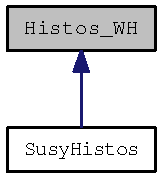
\includegraphics[width=114pt]{classHistos__WH__inherit__graph}
\end{center}
\end{figure}
\subsection*{Public Types}
\begin{DoxyCompactItemize}
\item 
\hypertarget{classHistos__WH_ab6f0f1c5fb37e2110a77c90f6069a0ab}{
typedef TH1F $\ast$ {\bfseries HDGWH} \mbox{[}WH\_\-NSR\mbox{]}\mbox{[}3\mbox{]}\mbox{[}DGSys\_\-N\mbox{]}}
\label{classHistos__WH_ab6f0f1c5fb37e2110a77c90f6069a0ab}

\end{DoxyCompactItemize}
\subsection*{Public Member Functions}
\begin{DoxyCompactItemize}
\item 
\hypertarget{classHistos__WH_afdd4095ad5a9266c7b99aefc25fd0415}{
void {\bfseries BookWHHistograms} (TDirectory $\ast$\_\-hDir, bool useSys=true)}
\label{classHistos__WH_afdd4095ad5a9266c7b99aefc25fd0415}

\item 
\hypertarget{classHistos__WH_a798824da17967b13857282ae8eacbc53}{
{\bfseries ClassDef} (\hyperlink{classHistos__WH}{Histos\_\-WH}, 1)}
\label{classHistos__WH_a798824da17967b13857282ae8eacbc53}

\end{DoxyCompactItemize}
\subsection*{Public Attributes}
\begin{DoxyCompactItemize}
\item 
\hypertarget{classHistos__WH_a5551c2f019da979d0736e055196df01e}{
TGuiUtils $\ast$ {\bfseries \_\-utils}}
\label{classHistos__WH_a5551c2f019da979d0736e055196df01e}

\item 
\hypertarget{classHistos__WH_a0783ffcbbfb55169dfd19a26dd725173}{
HDGWH {\bfseries DGWH\_\-pred}}
\label{classHistos__WH_a0783ffcbbfb55169dfd19a26dd725173}

\item 
\hypertarget{classHistos__WH_a944d8055d2149f4995e98d116a8d6b11}{
HDGWH {\bfseries DGWH\_\-cutflow}}
\label{classHistos__WH_a944d8055d2149f4995e98d116a8d6b11}

\item 
\hypertarget{classHistos__WH_a03cf361250042b4634b128775edc7f21}{
HDGWH {\bfseries DGWH\_\-nJets}}
\label{classHistos__WH_a03cf361250042b4634b128775edc7f21}

\item 
\hypertarget{classHistos__WH_a9c803d08322d492105b944a05a5e31fa}{
HDGWH {\bfseries DGWH\_\-nCJets}}
\label{classHistos__WH_a9c803d08322d492105b944a05a5e31fa}

\item 
\hypertarget{classHistos__WH_ac085d09bdc5d0a4b834f739e02bbec31}{
HDGWH {\bfseries DGWH\_\-nFJets}}
\label{classHistos__WH_ac085d09bdc5d0a4b834f739e02bbec31}

\item 
\hypertarget{classHistos__WH_ad318ae6444fb570db066d8a396efa93e}{
HDGWH {\bfseries DGWH\_\-nBJets}}
\label{classHistos__WH_ad318ae6444fb570db066d8a396efa93e}

\item 
\hypertarget{classHistos__WH_a09d6a39c4f520380afdaf6388f286172}{
HDGWH {\bfseries DGWH\_\-nSoftJets}}
\label{classHistos__WH_a09d6a39c4f520380afdaf6388f286172}

\item 
\hypertarget{classHistos__WH_a2afbaffd1be7d2bff0e3ccab547fa7bc}{
HDGWH {\bfseries DGWH\_\-qq}}
\label{classHistos__WH_a2afbaffd1be7d2bff0e3ccab547fa7bc}

\item 
\hypertarget{classHistos__WH_af21333b910c19f50de2cf024236793d9}{
HDGWH {\bfseries DGWH\_\-mll}}
\label{classHistos__WH_af21333b910c19f50de2cf024236793d9}

\item 
\hypertarget{classHistos__WH_a7a1f15cf4060583201bd304dc1526af1}{
HDGWH {\bfseries DGWH\_\-mllcoarse}}
\label{classHistos__WH_a7a1f15cf4060583201bd304dc1526af1}

\item 
\hypertarget{classHistos__WH_aa486216355d126fa2b29d04587f99b06}{
HDGWH {\bfseries DGWH\_\-mllcoarser}}
\label{classHistos__WH_aa486216355d126fa2b29d04587f99b06}

\item 
\hypertarget{classHistos__WH_af0f9708ac01b18a976c38429018df816}{
HDGWH {\bfseries DGWH\_\-mllShift}}
\label{classHistos__WH_af0f9708ac01b18a976c38429018df816}

\item 
\hypertarget{classHistos__WH_afb97eb537124a3dd0fa4c9789649b88b}{
HDGWH {\bfseries DGWH\_\-mjj}}
\label{classHistos__WH_afb97eb537124a3dd0fa4c9789649b88b}

\item 
\hypertarget{classHistos__WH_a87ec5d4bb87d4c291ac4adc099ced205}{
HDGWH {\bfseries DGWH\_\-pTll}}
\label{classHistos__WH_a87ec5d4bb87d4c291ac4adc099ced205}

\item 
\hypertarget{classHistos__WH_aa69e8e0f881a50ccdaf1a0f805766447}{
HDGWH {\bfseries DGWH\_\-mWWT}}
\label{classHistos__WH_aa69e8e0f881a50ccdaf1a0f805766447}

\item 
\hypertarget{classHistos__WH_a3b0b9cb75587484ab8c2058766582988}{
HDGWH {\bfseries DGWH\_\-dPhill}}
\label{classHistos__WH_a3b0b9cb75587484ab8c2058766582988}

\item 
\hypertarget{classHistos__WH_a496bba5ffbe739e3d6f44a80fd91d0c8}{
HDGWH {\bfseries DGWH\_\-dRll}}
\label{classHistos__WH_a496bba5ffbe739e3d6f44a80fd91d0c8}

\item 
\hypertarget{classHistos__WH_a47610b724c717a321da58fe2d1ae185c}{
HDGWH {\bfseries DGWH\_\-dEtall}}
\label{classHistos__WH_a47610b724c717a321da58fe2d1ae185c}

\item 
\hypertarget{classHistos__WH_ab6930e6c6988c0c19794012f8b31bebd}{
HDGWH {\bfseries DGWH\_\-dPhilMet}}
\label{classHistos__WH_ab6930e6c6988c0c19794012f8b31bebd}

\item 
\hypertarget{classHistos__WH_ab79b569a01935f194ca0c65fa8a0a781}{
HDGWH {\bfseries DGWH\_\-dPhiJetMet}}
\label{classHistos__WH_ab79b569a01935f194ca0c65fa8a0a781}

\item 
\hypertarget{classHistos__WH_afce0d98e835c1dccc96cb65311133f1c}{
HDGWH {\bfseries DGWH\_\-mTl1}}
\label{classHistos__WH_afce0d98e835c1dccc96cb65311133f1c}

\item 
\hypertarget{classHistos__WH_aaa6e6e6b78ad9998376339542dac5da4}{
HDGWH {\bfseries DGWH\_\-mTl2}}
\label{classHistos__WH_aaa6e6e6b78ad9998376339542dac5da4}

\item 
\hypertarget{classHistos__WH_a40e95e79548fc9bfa91783c5186ba701}{
HDGWH {\bfseries DGWH\_\-max\_\-mT}}
\label{classHistos__WH_a40e95e79548fc9bfa91783c5186ba701}

\item 
\hypertarget{classHistos__WH_a71e4d746c15294af9ea387da46698f3e}{
HDGWH {\bfseries DGWH\_\-JZBJet}}
\label{classHistos__WH_a71e4d746c15294af9ea387da46698f3e}

\item 
\hypertarget{classHistos__WH_a8c3ae95171078ecb29376396a35d6f42}{
HDGWH {\bfseries DGWH\_\-JZBEtmiss}}
\label{classHistos__WH_a8c3ae95171078ecb29376396a35d6f42}

\item 
\hypertarget{classHistos__WH_a9f6302e63926d676d1a0f341f1292bc2}{
HDGWH {\bfseries DGWH\_\-etmiss}}
\label{classHistos__WH_a9f6302e63926d676d1a0f341f1292bc2}

\item 
\hypertarget{classHistos__WH_ace92bea43b173cdf5a0785ae82fb85c6}{
HDGWH {\bfseries DGWH\_\-etmissPhi}}
\label{classHistos__WH_ace92bea43b173cdf5a0785ae82fb85c6}

\item 
\hypertarget{classHistos__WH_a04b0057e075601d613abe81378d8164e}{
HDGWH {\bfseries DGWH\_\-metrel}}
\label{classHistos__WH_a04b0057e075601d613abe81378d8164e}

\item 
\hypertarget{classHistos__WH_a42eb47a96c0bc218db297165e813dff5}{
HDGWH {\bfseries DGWH\_\-metrel1}}
\label{classHistos__WH_a42eb47a96c0bc218db297165e813dff5}

\item 
\hypertarget{classHistos__WH_ae5e6bedf80f0478ca7c394c92bdcb7b7}{
HDGWH {\bfseries DGWH\_\-metrel2}}
\label{classHistos__WH_ae5e6bedf80f0478ca7c394c92bdcb7b7}

\item 
\hypertarget{classHistos__WH_a9ea9b38c66d51981291af6df13043b70}{
HDGWH {\bfseries DGWH\_\-metrel3}}
\label{classHistos__WH_a9ea9b38c66d51981291af6df13043b70}

\item 
\hypertarget{classHistos__WH_a066c3842380d8e6b821e69d27b29a046}{
HDGWH {\bfseries DGWH\_\-metRefEle}}
\label{classHistos__WH_a066c3842380d8e6b821e69d27b29a046}

\item 
\hypertarget{classHistos__WH_afefad233291f8838c927198b1b6a7e9f}{
HDGWH {\bfseries DGWH\_\-metRefGam}}
\label{classHistos__WH_afefad233291f8838c927198b1b6a7e9f}

\item 
\hypertarget{classHistos__WH_aa24d650d8784d6f3ee116ea3fce60dac}{
HDGWH {\bfseries DGWH\_\-metRefMuo}}
\label{classHistos__WH_aa24d650d8784d6f3ee116ea3fce60dac}

\item 
\hypertarget{classHistos__WH_a3c3706042e90a197f3d47cacd0fdf7eb}{
HDGWH {\bfseries DGWH\_\-metRefJet}}
\label{classHistos__WH_a3c3706042e90a197f3d47cacd0fdf7eb}

\item 
\hypertarget{classHistos__WH_ad0ed0b35c6ed86341fdde56f1e354ed2}{
HDGWH {\bfseries DGWH\_\-metRefSJet}}
\label{classHistos__WH_ad0ed0b35c6ed86341fdde56f1e354ed2}

\item 
\hypertarget{classHistos__WH_a082747d4455a0b2c236f50dfc4781ccc}{
HDGWH {\bfseries DGWH\_\-metCellout}}
\label{classHistos__WH_a082747d4455a0b2c236f50dfc4781ccc}

\item 
\hypertarget{classHistos__WH_a9896d9d9e0aa63942a0a8550a5e1464f}{
HDGWH {\bfseries DGWH\_\-mt2}}
\label{classHistos__WH_a9896d9d9e0aa63942a0a8550a5e1464f}

\item 
\hypertarget{classHistos__WH_a3e0ab6f2be8011fb54b0deb6d432f5fa}{
HDGWH {\bfseries DGWH\_\-mt2b}}
\label{classHistos__WH_a3e0ab6f2be8011fb54b0deb6d432f5fa}

\item 
\hypertarget{classHistos__WH_af4eb53ba0ec7225eb85041651fbdb8cc}{
HDGWH {\bfseries DGWH\_\-mt2j}}
\label{classHistos__WH_af4eb53ba0ec7225eb85041651fbdb8cc}

\item 
\hypertarget{classHistos__WH_aeaadc529ec7e4b437ae8a44f0f66db30}{
HDGWH {\bfseries DGWH\_\-mlj}}
\label{classHistos__WH_aeaadc529ec7e4b437ae8a44f0f66db30}

\item 
\hypertarget{classHistos__WH_adae271892519be0f367b438c001664d5}{
HDGWH {\bfseries DGWH\_\-mljj}}
\label{classHistos__WH_adae271892519be0f367b438c001664d5}

\item 
\hypertarget{classHistos__WH_a3c7701f528aab53938d67356dccd89a4}{
HDGWH {\bfseries DGWH\_\-mEff}}
\label{classHistos__WH_a3c7701f528aab53938d67356dccd89a4}

\item 
\hypertarget{classHistos__WH_afb7db70f3acf4e2473cade45f1ec7979}{
HDGWH {\bfseries DGWH\_\-ST}}
\label{classHistos__WH_afb7db70f3acf4e2473cade45f1ec7979}

\item 
\hypertarget{classHistos__WH_ae4f252b30dda93ae2458bdd16a9578e5}{
HDGWH {\bfseries DGWH\_\-MetSig}}
\label{classHistos__WH_ae4f252b30dda93ae2458bdd16a9578e5}

\item 
\hypertarget{classHistos__WH_a6b40c6b423f28ca6063311dcd6fc9e83}{
HDGWH {\bfseries DGWH\_\-npv}}
\label{classHistos__WH_a6b40c6b423f28ca6063311dcd6fc9e83}

\item 
\hypertarget{classHistos__WH_aae2c7fd2eaf09660064e476e14daec1e}{
HDGWH {\bfseries DGWH\_\-mu}}
\label{classHistos__WH_aae2c7fd2eaf09660064e476e14daec1e}

\item 
\hypertarget{classHistos__WH_ab4b4b64dfaf1f0a05d35596d7c16c6c1}{
HDGWH {\bfseries DGWH\_\-ptl1}}
\label{classHistos__WH_ab4b4b64dfaf1f0a05d35596d7c16c6c1}

\item 
\hypertarget{classHistos__WH_a5e02db3ac8e8101f3f94b01715182430}{
HDGWH {\bfseries DGWH\_\-ptl2}}
\label{classHistos__WH_a5e02db3ac8e8101f3f94b01715182430}

\item 
\hypertarget{classHistos__WH_ae5442f3fd21df6161e3679756166db1a}{
HDGWH {\bfseries DGWH\_\-etal1}}
\label{classHistos__WH_ae5442f3fd21df6161e3679756166db1a}

\item 
\hypertarget{classHistos__WH_acdbeed5ac2693831845bd5a53e9cb626}{
HDGWH {\bfseries DGWH\_\-etal2}}
\label{classHistos__WH_acdbeed5ac2693831845bd5a53e9cb626}

\item 
\hypertarget{classHistos__WH_a53a4f1cfbe983c8fdc7ef2ef0e265d74}{
HDGWH {\bfseries DGWH\_\-ePt}}
\label{classHistos__WH_a53a4f1cfbe983c8fdc7ef2ef0e265d74}

\item 
\hypertarget{classHistos__WH_a1912ee044af00a9a69490e377ca8e0f6}{
HDGWH {\bfseries DGWH\_\-mPt}}
\label{classHistos__WH_a1912ee044af00a9a69490e377ca8e0f6}

\item 
\hypertarget{classHistos__WH_add11f74dc7c6c92841e53b77a473fd53}{
HDGWH {\bfseries DGWH\_\-eEta}}
\label{classHistos__WH_add11f74dc7c6c92841e53b77a473fd53}

\item 
\hypertarget{classHistos__WH_a3bf55ff62086327c829464bafc167f3c}{
HDGWH {\bfseries DGWH\_\-mEta}}
\label{classHistos__WH_a3bf55ff62086327c829464bafc167f3c}

\item 
\hypertarget{classHistos__WH_ae1a9c98b67eeea10cbe6b474dd3b0f2b}{
HDGWH {\bfseries DGWH\_\-d0Sl1}}
\label{classHistos__WH_ae1a9c98b67eeea10cbe6b474dd3b0f2b}

\item 
\hypertarget{classHistos__WH_aa6e4862894f54f42629f1597cd9ed527}{
HDGWH {\bfseries DGWH\_\-d0Sl2}}
\label{classHistos__WH_aa6e4862894f54f42629f1597cd9ed527}

\item 
\hypertarget{classHistos__WH_a4a8600c5dacad07e2243dab73a60a17b}{
HDGWH {\bfseries DGWH\_\-z0sinthetal1}}
\label{classHistos__WH_a4a8600c5dacad07e2243dab73a60a17b}

\item 
\hypertarget{classHistos__WH_abe75d28abe692d1965774daadf755c54}{
HDGWH {\bfseries DGWH\_\-z0sinthetal2}}
\label{classHistos__WH_abe75d28abe692d1965774daadf755c54}

\item 
\hypertarget{classHistos__WH_ac9ac5e61616a4ef51d3696e87ae853aa}{
HDGWH {\bfseries DGWH\_\-orgl1}}
\label{classHistos__WH_ac9ac5e61616a4ef51d3696e87ae853aa}

\item 
\hypertarget{classHistos__WH_ac48e2237a5ccdce54cee7af12c8b1075}{
HDGWH {\bfseries DGWH\_\-orgl2}}
\label{classHistos__WH_ac48e2237a5ccdce54cee7af12c8b1075}

\item 
\hypertarget{classHistos__WH_acd318b7fd149781d9bcdea0152c601ea}{
HDGWH {\bfseries DGWH\_\-ptj1}}
\label{classHistos__WH_acd318b7fd149781d9bcdea0152c601ea}

\item 
\hypertarget{classHistos__WH_ace635607f7a26f89bd7be64599b1271f}{
HDGWH {\bfseries DGWH\_\-ptj2}}
\label{classHistos__WH_ace635607f7a26f89bd7be64599b1271f}

\item 
\hypertarget{classHistos__WH_a5c5261c99c7b512acbe2e3dd95714b0b}{
HDGWH {\bfseries DGWH\_\-ptj3}}
\label{classHistos__WH_a5c5261c99c7b512acbe2e3dd95714b0b}

\item 
\hypertarget{classHistos__WH_ace909f55037a60cfb04f0442250341f3}{
HDGWH {\bfseries DGWH\_\-ptj4}}
\label{classHistos__WH_ace909f55037a60cfb04f0442250341f3}

\item 
\hypertarget{classHistos__WH_a86b01f7a3a41b21dbbf4d1a5db1c0f6b}{
HDGWH {\bfseries DGWH\_\-etaj1}}
\label{classHistos__WH_a86b01f7a3a41b21dbbf4d1a5db1c0f6b}

\item 
\hypertarget{classHistos__WH_adf1279dc7fabf8ca179ac0f2a03b0b0d}{
HDGWH {\bfseries DGWH\_\-etaj2}}
\label{classHistos__WH_adf1279dc7fabf8ca179ac0f2a03b0b0d}

\item 
\hypertarget{classHistos__WH_aafa3fddeb7045a5eb46cc57945c72458}{
HDGWH {\bfseries DGWH\_\-etaj3}}
\label{classHistos__WH_aafa3fddeb7045a5eb46cc57945c72458}

\item 
\hypertarget{classHistos__WH_a82bb07a1b4359bc44a67efe974b5c318}{
HDGWH {\bfseries DGWH\_\-etaj4}}
\label{classHistos__WH_a82bb07a1b4359bc44a67efe974b5c318}

\item 
\hypertarget{classHistos__WH_ae87107eadeeb09515b3d87e409975467}{
HDGWH {\bfseries DGWH\_\-jvfj1}}
\label{classHistos__WH_ae87107eadeeb09515b3d87e409975467}

\item 
\hypertarget{classHistos__WH_a257882d93a88565ded3d22fe86d00f91}{
HDGWH {\bfseries DGWH\_\-jvfj2}}
\label{classHistos__WH_a257882d93a88565ded3d22fe86d00f91}

\item 
\hypertarget{classHistos__WH_adec9645eb199d0b7906b8bd2c3c711cd}{
HDGWH {\bfseries DGWH\_\-ptbj}}
\label{classHistos__WH_adec9645eb199d0b7906b8bd2c3c711cd}

\item 
\hypertarget{classHistos__WH_a165dd5a978ea215372c4625062c48905}{
HDGWH {\bfseries DGWH\_\-etabj}}
\label{classHistos__WH_a165dd5a978ea215372c4625062c48905}

\item 
\hypertarget{classHistos__WH_a7a7ac4faf351c92a36a9e067abe78424}{
HDGWH {\bfseries DGWH\_\-jvfbj}}
\label{classHistos__WH_a7a7ac4faf351c92a36a9e067abe78424}

\item 
\hypertarget{classHistos__WH_a4d11a521d00a428b400a6a5f36d561e8}{
HDGWH {\bfseries DGWH\_\-ptSj1}}
\label{classHistos__WH_a4d11a521d00a428b400a6a5f36d561e8}

\item 
\hypertarget{classHistos__WH_ab579a15ab0bd413c5028898cece44deb}{
HDGWH {\bfseries DGWH\_\-ptSj2}}
\label{classHistos__WH_ab579a15ab0bd413c5028898cece44deb}

\item 
\hypertarget{classHistos__WH_a105be6a5e44eb05d6b5f2d4e8de60746}{
HDGWH {\bfseries DGWH\_\-etaSj1}}
\label{classHistos__WH_a105be6a5e44eb05d6b5f2d4e8de60746}

\item 
\hypertarget{classHistos__WH_a83809a93b7013e372601f0802f174c62}{
HDGWH {\bfseries DGWH\_\-etaSj2}}
\label{classHistos__WH_a83809a93b7013e372601f0802f174c62}

\item 
\hypertarget{classHistos__WH_afc3ba7412dbfa6e177a1f0293a690180}{
HDGWH {\bfseries DGWH\_\-jvfSj1}}
\label{classHistos__WH_afc3ba7412dbfa6e177a1f0293a690180}

\item 
\hypertarget{classHistos__WH_a4d14deed8b028f30728c26f7a1786ee1}{
HDGWH {\bfseries DGWH\_\-jvfSj2}}
\label{classHistos__WH_a4d14deed8b028f30728c26f7a1786ee1}

\end{DoxyCompactItemize}


The documentation for this class was generated from the following files:\begin{DoxyCompactItemize}
\item 
SusyWeakProdAna/Histos\_\-WH.h\item 
Root/Histos\_\-WH.cxx\end{DoxyCompactItemize}

\hypertarget{classsl__File}{
\section{sl\_\-File Class Reference}
\label{classsl__File}\index{sl\_\-File@{sl\_\-File}}
}
\subsection*{Public Member Functions}
\begin{DoxyCompactItemize}
\item 
\hypertarget{classsl__File_a4b82007051fc943491d4176ef5cf8a6f}{
{\bfseries sl\_\-File} (int id, float m\_\-susy, float m\_\-neutralino, string f\_\-name, float xs=0, float xsSys=0)}
\label{classsl__File_a4b82007051fc943491d4176ef5cf8a6f}

\item 
\hypertarget{classsl__File_a6d607f0faa8917f709622d59e74e9158}{
int {\bfseries getId} ()}
\label{classsl__File_a6d607f0faa8917f709622d59e74e9158}

\item 
\hypertarget{classsl__File_adaeef5c2fbe0f7a83425dfe072b3226e}{
float {\bfseries getSusyMass} ()}
\label{classsl__File_adaeef5c2fbe0f7a83425dfe072b3226e}

\item 
\hypertarget{classsl__File_ae86f3d64d389dec1de380e05aa310507}{
float {\bfseries getNeutralinoMass} ()}
\label{classsl__File_ae86f3d64d389dec1de380e05aa310507}

\item 
\hypertarget{classsl__File_a1d7827232888e25964983bdf1480b5a2}{
string {\bfseries getFName} ()}
\label{classsl__File_a1d7827232888e25964983bdf1480b5a2}

\item 
\hypertarget{classsl__File_a6b0d73263c1f8f014502300096d8320d}{
float {\bfseries getXS} ()}
\label{classsl__File_a6b0d73263c1f8f014502300096d8320d}

\item 
\hypertarget{classsl__File_a220fe7bacdeee19347057e4f652ba9b1}{
float {\bfseries getXSsys} ()}
\label{classsl__File_a220fe7bacdeee19347057e4f652ba9b1}

\end{DoxyCompactItemize}


The documentation for this class was generated from the following file:\begin{DoxyCompactItemize}
\item 
SusyWeakProdAna/SROptimization.h\end{DoxyCompactItemize}

\hypertarget{classSROptimization}{
\section{SROptimization Class Reference}
\label{classSROptimization}\index{SROptimization@{SROptimization}}
}
\subsection*{Public Member Functions}
\begin{DoxyCompactItemize}
\item 
\hypertarget{classSROptimization_a272576b1a7c21e8292e255da28d74185}{
{\bfseries SROptimization} (RegionOption option, SusyProcess sp, string skim, string dilType=\char`\"{}ALL\char`\"{})}
\label{classSROptimization_a272576b1a7c21e8292e255da28d74185}

\item 
\hypertarget{classSROptimization_a68dc648f509c7e69aa84db765ae97e9d}{
void {\bfseries setDebug} (int d)}
\label{classSROptimization_a68dc648f509c7e69aa84db765ae97e9d}

\item 
\hypertarget{classSROptimization_ad7ae794f3337548c86580d7f8cfb204e}{
void {\bfseries init} ()}
\label{classSROptimization_ad7ae794f3337548c86580d7f8cfb204e}

\item 
\hypertarget{classSROptimization_a801db8bf09ddba833864e595e7e1c189}{
void {\bfseries PlotSig} ()}
\label{classSROptimization_a801db8bf09ddba833864e595e7e1c189}

\item 
\hypertarget{classSROptimization_aaeece2802ac00819357d520954c77f72}{
void {\bfseries PlotMaxSig} ()}
\label{classSROptimization_aaeece2802ac00819357d520954c77f72}

\item 
\hypertarget{classSROptimization_aff182e4ed79b8b9f85d668c6a0333bfe}{
void {\bfseries dumpBkgTable} ()}
\label{classSROptimization_aff182e4ed79b8b9f85d668c6a0333bfe}

\item 
\hypertarget{classSROptimization_aa735b2b43492fccef287a09fa79c11ca}{
void {\bfseries dumpSignalTable} ()}
\label{classSROptimization_aa735b2b43492fccef287a09fa79c11ca}

\item 
\hypertarget{classSROptimization_a4b5f3e94d487d12c091e0369461d0c12}{
void {\bfseries combineZn} ()}
\label{classSROptimization_a4b5f3e94d487d12c091e0369461d0c12}

\end{DoxyCompactItemize}


The documentation for this class was generated from the following files:\begin{DoxyCompactItemize}
\item 
SusyWeakProdAna/SROptimization.h\item 
Root/SROptimization.cxx\end{DoxyCompactItemize}

\hypertarget{classSusy2LepAna}{
\section{Susy2LepAna Class Reference}
\label{classSusy2LepAna}\index{Susy2LepAna@{Susy2LepAna}}
}
Inheritance diagram for Susy2LepAna:\nopagebreak
\begin{figure}[H]
\begin{center}
\leavevmode
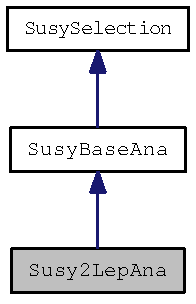
\includegraphics[width=130pt]{classSusy2LepAna__inherit__graph}
\end{center}
\end{figure}
Collaboration diagram for Susy2LepAna:\nopagebreak
\begin{figure}[H]
\begin{center}
\leavevmode
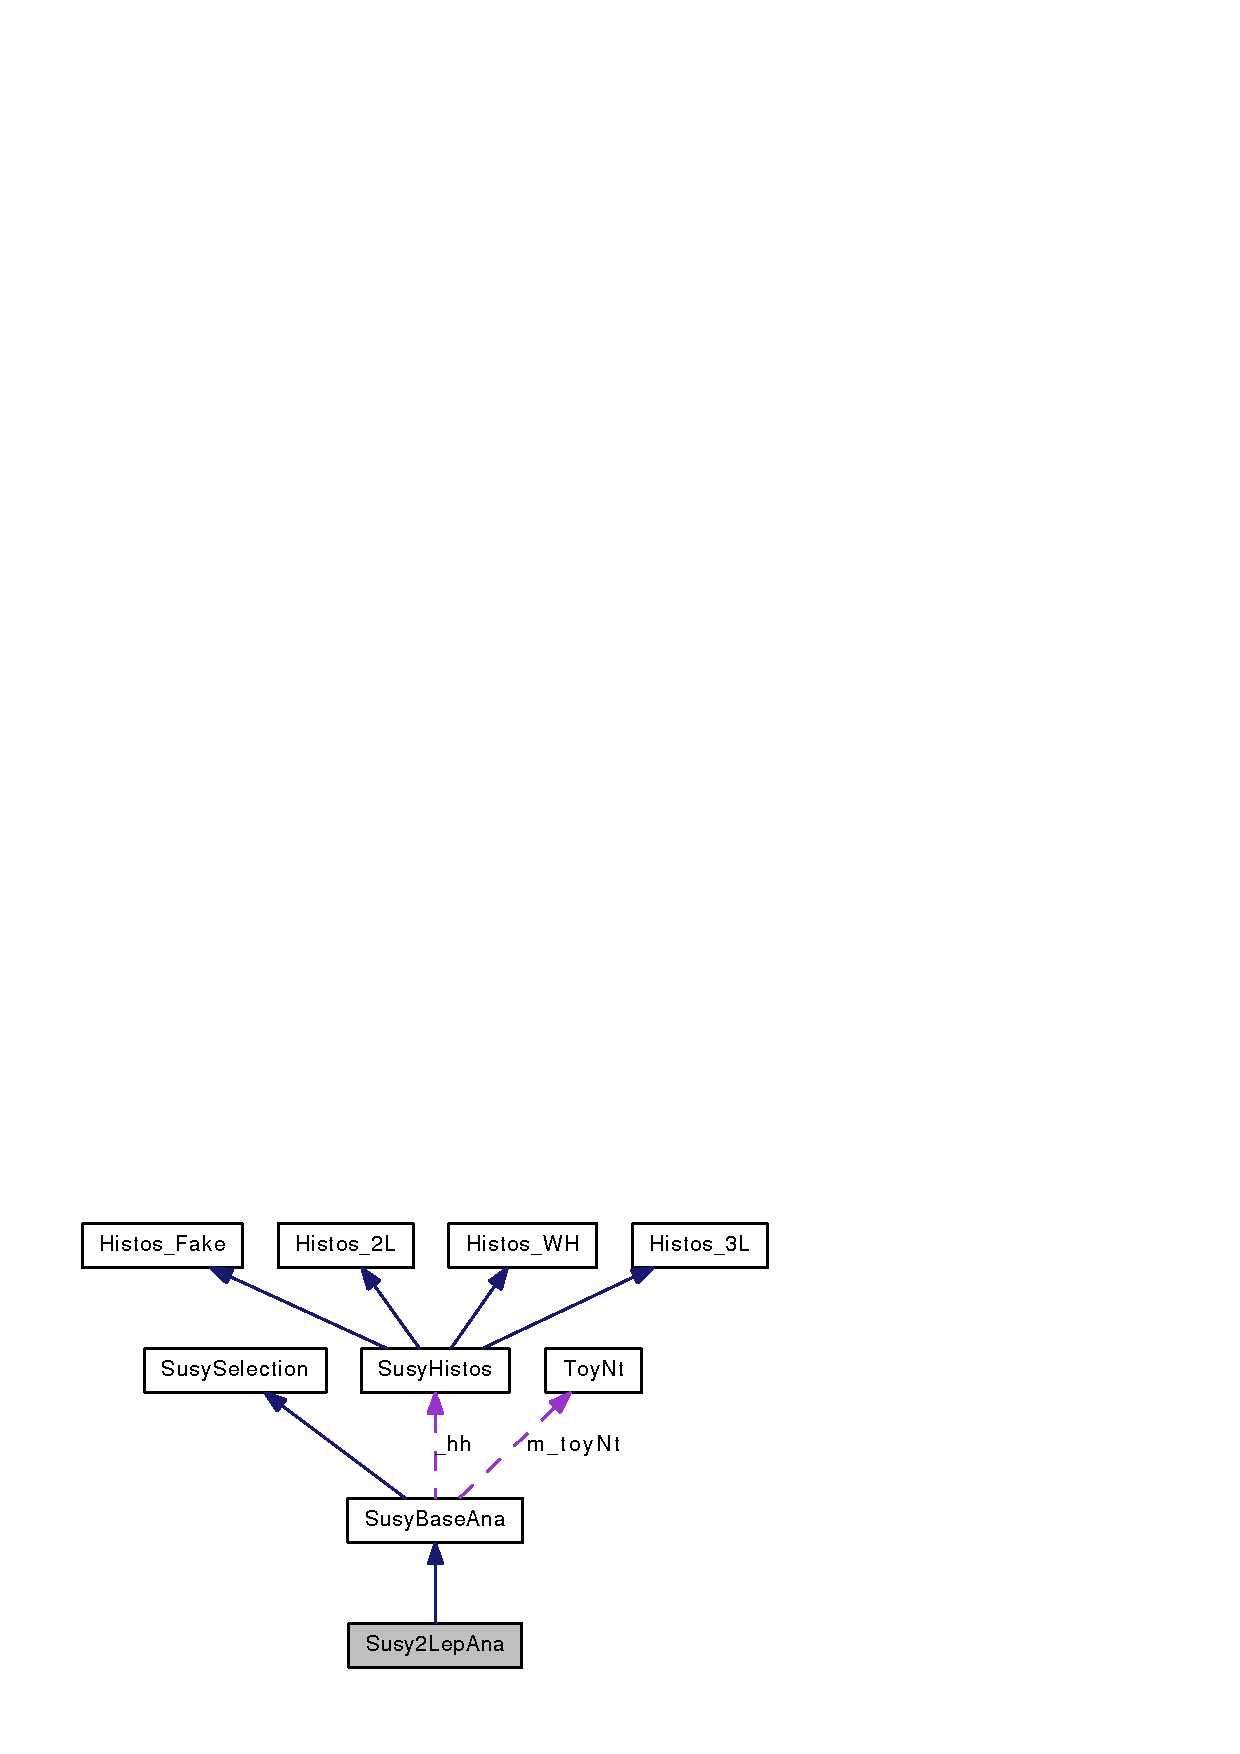
\includegraphics[width=372pt]{classSusy2LepAna__coll__graph}
\end{center}
\end{figure}
\subsection*{Public Member Functions}
\begin{DoxyCompactItemize}
\item 
\hypertarget{classSusy2LepAna_a0237540d04fdc88c660b0caa57358dd2}{
{\bfseries Susy2LepAna} (\hyperlink{classSusyHistos}{SusyHistos} $\ast$\_\-histos)}
\label{classSusy2LepAna_a0237540d04fdc88c660b0caa57358dd2}

\item 
\hypertarget{classSusy2LepAna_a5be35d360519d524621450274f4a3d37}{
float {\bfseries getFakeWeight} (const LeptonVector $\ast$leptons, uint nVtx, bool isMC, int iSR, float metrel, uint iSys=DGSys\_\-NOM)}
\label{classSusy2LepAna_a5be35d360519d524621450274f4a3d37}

\item 
\hypertarget{classSusy2LepAna_a4b79edbd172829545eedb035414636ad}{
void {\bfseries doAnalysis} (float w, unsigned int isys=DGSys\_\-NOM)}
\label{classSusy2LepAna_a4b79edbd172829545eedb035414636ad}

\item 
\hypertarget{classSusy2LepAna_ae005ac716d400f5bead2d5a72e0c0a95}{
void {\bfseries end} ()}
\label{classSusy2LepAna_ae005ac716d400f5bead2d5a72e0c0a95}

\item 
\hypertarget{classSusy2LepAna_a1e90ba8b63135cd2d10a80b58043a171}{
void {\bfseries setSelection} (std::string s, uint dilType)}
\label{classSusy2LepAna_a1e90ba8b63135cd2d10a80b58043a171}

\item 
\hypertarget{classSusy2LepAna_ab5da399f55f2a125e9f267da7941575e}{
bool {\bfseries selectEvent} (LeptonVector $\ast$leptons, LeptonVector $\ast$baseLeptons, const JetVector $\ast$jets, const Met $\ast$met, float w)}
\label{classSusy2LepAna_ab5da399f55f2a125e9f267da7941575e}

\item 
\hypertarget{classSusy2LepAna_a8609fc82111b8c7b785cdfe2c53712a6}{
void {\bfseries fillHistograms} (uint iSR, uint iSYS, const LeptonVector $\ast$leptons, const JetVector $\ast$jets, const Met $\ast$met, float \_\-ww)}
\label{classSusy2LepAna_a8609fc82111b8c7b785cdfe2c53712a6}

\item 
\hypertarget{classSusy2LepAna_aedb67994c4929809a52c75505868046b}{
void {\bfseries initializeHistFitterTree} ()}
\label{classSusy2LepAna_aedb67994c4929809a52c75505868046b}

\item 
\hypertarget{classSusy2LepAna_a1a0d2b619104ffc129b7378d0ad78aa3}{
float {\bfseries writeIntoHistFitterTree} (uint iSR, LeptonVector $\ast$leptons, const LeptonVector $\ast$baseLeptons, const JetVector $\ast$signalJets, const JetVector $\ast$baseJets, const Met $\ast$met)}
\label{classSusy2LepAna_a1a0d2b619104ffc129b7378d0ad78aa3}

\item 
\hypertarget{classSusy2LepAna_ae8dd26f0b33cb51f17c5154d8987d90a}{
bool {\bfseries validSystForHFT} (uint iSR)}
\label{classSusy2LepAna_ae8dd26f0b33cb51f17c5154d8987d90a}

\item 
\hypertarget{classSusy2LepAna_ac72ae5958184ca2594786e279466e51a}{
void {\bfseries moveHFTOutput} ()}
\label{classSusy2LepAna_ac72ae5958184ca2594786e279466e51a}

\item 
\hypertarget{classSusy2LepAna_ab92b69085553cec932f1d852828a27b1}{
void {\bfseries print\_\-SRmT2} ()}
\label{classSusy2LepAna_ab92b69085553cec932f1d852828a27b1}

\item 
\hypertarget{classSusy2LepAna_aa313308520befbf3059f31b50114a19d}{
void {\bfseries print\_\-SRWW} ()}
\label{classSusy2LepAna_aa313308520befbf3059f31b50114a19d}

\item 
\hypertarget{classSusy2LepAna_a94e9f02c276646d82833e45f20b75ec0}{
void {\bfseries print\_\-SRZjets} ()}
\label{classSusy2LepAna_a94e9f02c276646d82833e45f20b75ec0}

\item 
\hypertarget{classSusy2LepAna_a713ed7fec5d1c8cef9ec8db3740d0f99}{
void {\bfseries print\_\-SRSSjets} ()}
\label{classSusy2LepAna_a713ed7fec5d1c8cef9ec8db3740d0f99}

\item 
\hypertarget{classSusy2LepAna_ae98d6a9bd56a7a72a3e1a725a72d23ee}{
void {\bfseries print\_\-WWCR} ()}
\label{classSusy2LepAna_ae98d6a9bd56a7a72a3e1a725a72d23ee}

\item 
\hypertarget{classSusy2LepAna_a3b4a54efb897c0ff83001416b46c7b47}{
void {\bfseries print\_\-TOPCR} ()}
\label{classSusy2LepAna_a3b4a54efb897c0ff83001416b46c7b47}

\item 
\hypertarget{classSusy2LepAna_a8778301326d981a8cf1697761998f54a}{
void {\bfseries print\_\-ZVCR} ()}
\label{classSusy2LepAna_a8778301326d981a8cf1697761998f54a}

\item 
\hypertarget{classSusy2LepAna_af4e0741b5f83f1e1843d5b52a2d79153}{
void {\bfseries print\_\-VRSS} ()}
\label{classSusy2LepAna_af4e0741b5f83f1e1843d5b52a2d79153}

\item 
\hypertarget{classSusy2LepAna_aec04d7ad73e705c21eaa19135237c3c6}{
void {\bfseries print\_\-CRZ} ()}
\label{classSusy2LepAna_aec04d7ad73e705c21eaa19135237c3c6}

\item 
\hypertarget{classSusy2LepAna_a62ec3a44d0b55bee59ab3ea72e869425}{
{\bfseries ClassDef} (\hyperlink{classSusy2LepAna}{Susy2LepAna}, 1)}
\label{classSusy2LepAna_a62ec3a44d0b55bee59ab3ea72e869425}

\end{DoxyCompactItemize}
\subsection*{Protected Attributes}
\begin{DoxyCompactItemize}
\item 
\hypertarget{classSusy2LepAna_ad0141ca9740e4671a0b8e14127b3878e}{
HistFitterTree $\ast$ {\bfseries m\_\-histFitterTrees} \mbox{[}DGSys\_\-GEN\mbox{]}}
\label{classSusy2LepAna_ad0141ca9740e4671a0b8e14127b3878e}

\item 
\hypertarget{classSusy2LepAna_a2c84893e90fc06d4ee53e0d1929b1636}{
bool {\bfseries m\_\-writeHFT}}
\label{classSusy2LepAna_a2c84893e90fc06d4ee53e0d1929b1636}

\item 
\hypertarget{classSusy2LepAna_ac2de9c96ade4fd1b6b1adf714eae0f9c}{
string {\bfseries HFTName}}
\label{classSusy2LepAna_ac2de9c96ade4fd1b6b1adf714eae0f9c}

\end{DoxyCompactItemize}


The documentation for this class was generated from the following files:\begin{DoxyCompactItemize}
\item 
SusyWeakProdAna/Susy2LepAna.h\item 
Root/Susy2LepAna.cxx\end{DoxyCompactItemize}

\hypertarget{classSusy3LepAna}{
\section{Susy3LepAna Class Reference}
\label{classSusy3LepAna}\index{Susy3LepAna@{Susy3LepAna}}
}
Inheritance diagram for Susy3LepAna:\nopagebreak
\begin{figure}[H]
\begin{center}
\leavevmode
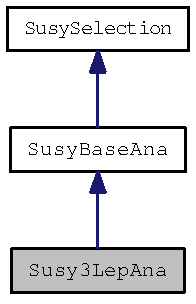
\includegraphics[width=130pt]{classSusy3LepAna__inherit__graph}
\end{center}
\end{figure}
Collaboration diagram for Susy3LepAna:\nopagebreak
\begin{figure}[H]
\begin{center}
\leavevmode
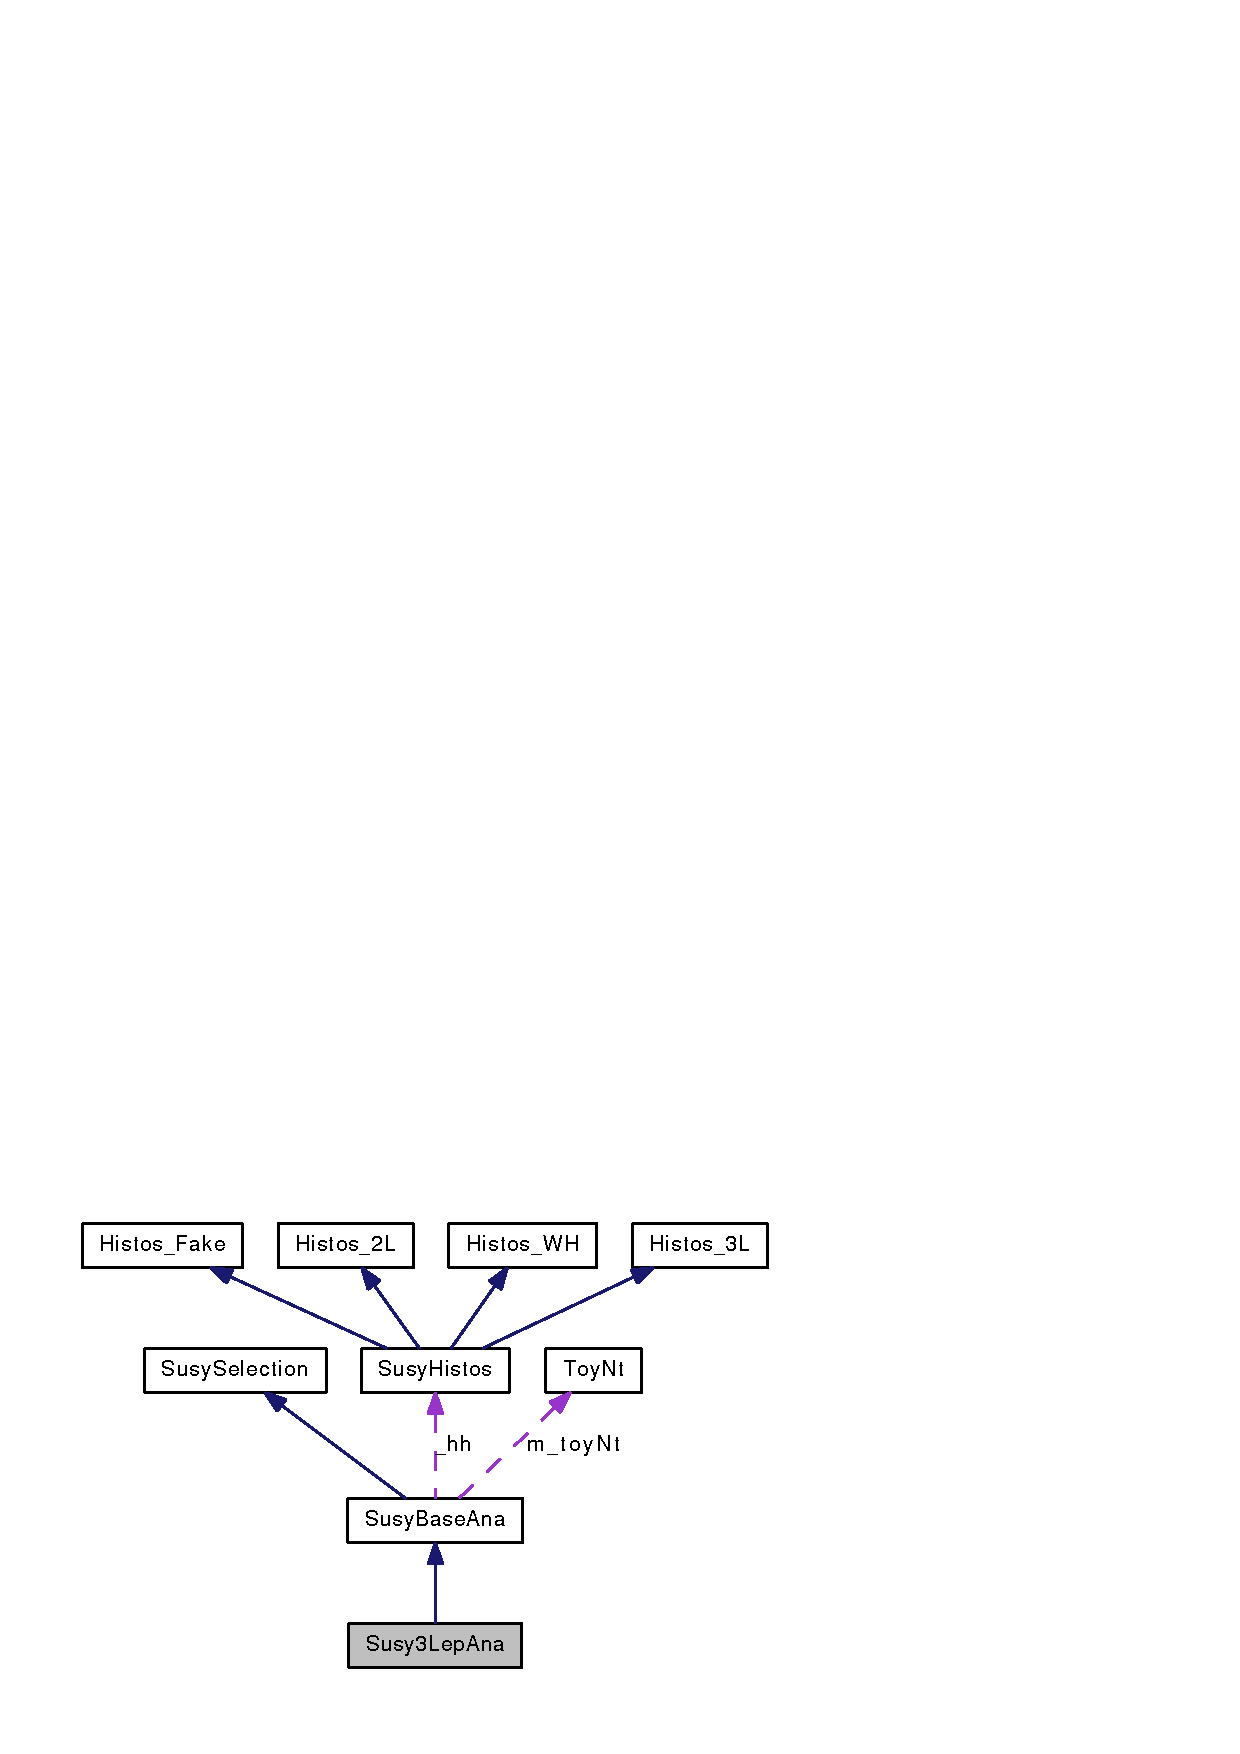
\includegraphics[width=372pt]{classSusy3LepAna__coll__graph}
\end{center}
\end{figure}
\subsection*{Public Member Functions}
\begin{DoxyCompactItemize}
\item 
\hypertarget{classSusy3LepAna_af58b46d32a1d7807474b2d39e3185965}{
{\bfseries Susy3LepAna} (\hyperlink{classSusyHistos}{SusyHistos} $\ast$\_\-histos)}
\label{classSusy3LepAna_af58b46d32a1d7807474b2d39e3185965}

\item 
\hypertarget{classSusy3LepAna_a064dde13f4c15d9cfe13c3fdb55c7948}{
void {\bfseries doAnalysis} (float w, unsigned int isys)}
\label{classSusy3LepAna_a064dde13f4c15d9cfe13c3fdb55c7948}

\item 
\hypertarget{classSusy3LepAna_ae76031474c2b58200b9afc3f4fedc3e2}{
bool {\bfseries selectEvent} (LeptonVector $\ast$leptons, const TauVector $\ast$taus, const JetVector $\ast$jets, const Susy::Met $\ast$met, float w)}
\label{classSusy3LepAna_ae76031474c2b58200b9afc3f4fedc3e2}

\item 
\hypertarget{classSusy3LepAna_adc0ca250af87072b6209a244a60fa201}{
void {\bfseries setSelection} (std::string s)}
\label{classSusy3LepAna_adc0ca250af87072b6209a244a60fa201}

\item 
\hypertarget{classSusy3LepAna_a01eebce66c9961fc9aa3c48e29ee5666}{
void {\bfseries end} ()}
\label{classSusy3LepAna_a01eebce66c9961fc9aa3c48e29ee5666}

\item 
\hypertarget{classSusy3LepAna_a3d3223ba50e7dd182a0806191623115e}{
void {\bfseries fillHistograms} (uint iSR, uint iSYS, const LeptonVector $\ast$leptons, const JetVector $\ast$jets, const Susy::Met $\ast$met, float \_\-ww)}
\label{classSusy3LepAna_a3d3223ba50e7dd182a0806191623115e}

\item 
\hypertarget{classSusy3LepAna_adb2dde7ccb257b40d8148614db8e1533}{
int {\bfseries evtCatgUnOrd} (const LeptonVector $\ast$leptons)}
\label{classSusy3LepAna_adb2dde7ccb257b40d8148614db8e1533}

\item 
\hypertarget{classSusy3LepAna_a73adef000977472c81ca4d683d09697a}{
int {\bfseries evtCatgOrd} (const LeptonVector $\ast$leptons, bool useOS)}
\label{classSusy3LepAna_a73adef000977472c81ca4d683d09697a}

\item 
\hypertarget{classSusy3LepAna_afced64a093df64665e591616388c40f4}{
void {\bfseries print\_\-CF3L} ()}
\label{classSusy3LepAna_afced64a093df64665e591616388c40f4}

\item 
\hypertarget{classSusy3LepAna_a257c6f378c2ba37fc0f5c06e8f2042e8}{
void {\bfseries print\_\-VRWZ} ()}
\label{classSusy3LepAna_a257c6f378c2ba37fc0f5c06e8f2042e8}

\item 
\hypertarget{classSusy3LepAna_a9b928e56d8c0e8574562296cb0eac387}{
void {\bfseries print\_\-VRZZ} ()}
\label{classSusy3LepAna_a9b928e56d8c0e8574562296cb0eac387}

\item 
\hypertarget{classSusy3LepAna_a5be9542d641e88e6848eef3732572b05}{
{\bfseries ClassDef} (\hyperlink{classSusy3LepAna}{Susy3LepAna}, 1)}
\label{classSusy3LepAna_a5be9542d641e88e6848eef3732572b05}

\end{DoxyCompactItemize}


The documentation for this class was generated from the following files:\begin{DoxyCompactItemize}
\item 
SusyWeakProdAna/Susy3LepAna.h\item 
Root/Susy3LepAna.cxx\end{DoxyCompactItemize}

\hypertarget{classSusyAnaLooper}{
\section{SusyAnaLooper Class Reference}
\label{classSusyAnaLooper}\index{SusyAnaLooper@{SusyAnaLooper}}
}
Collaboration diagram for SusyAnaLooper:\nopagebreak
\begin{figure}[H]
\begin{center}
\leavevmode
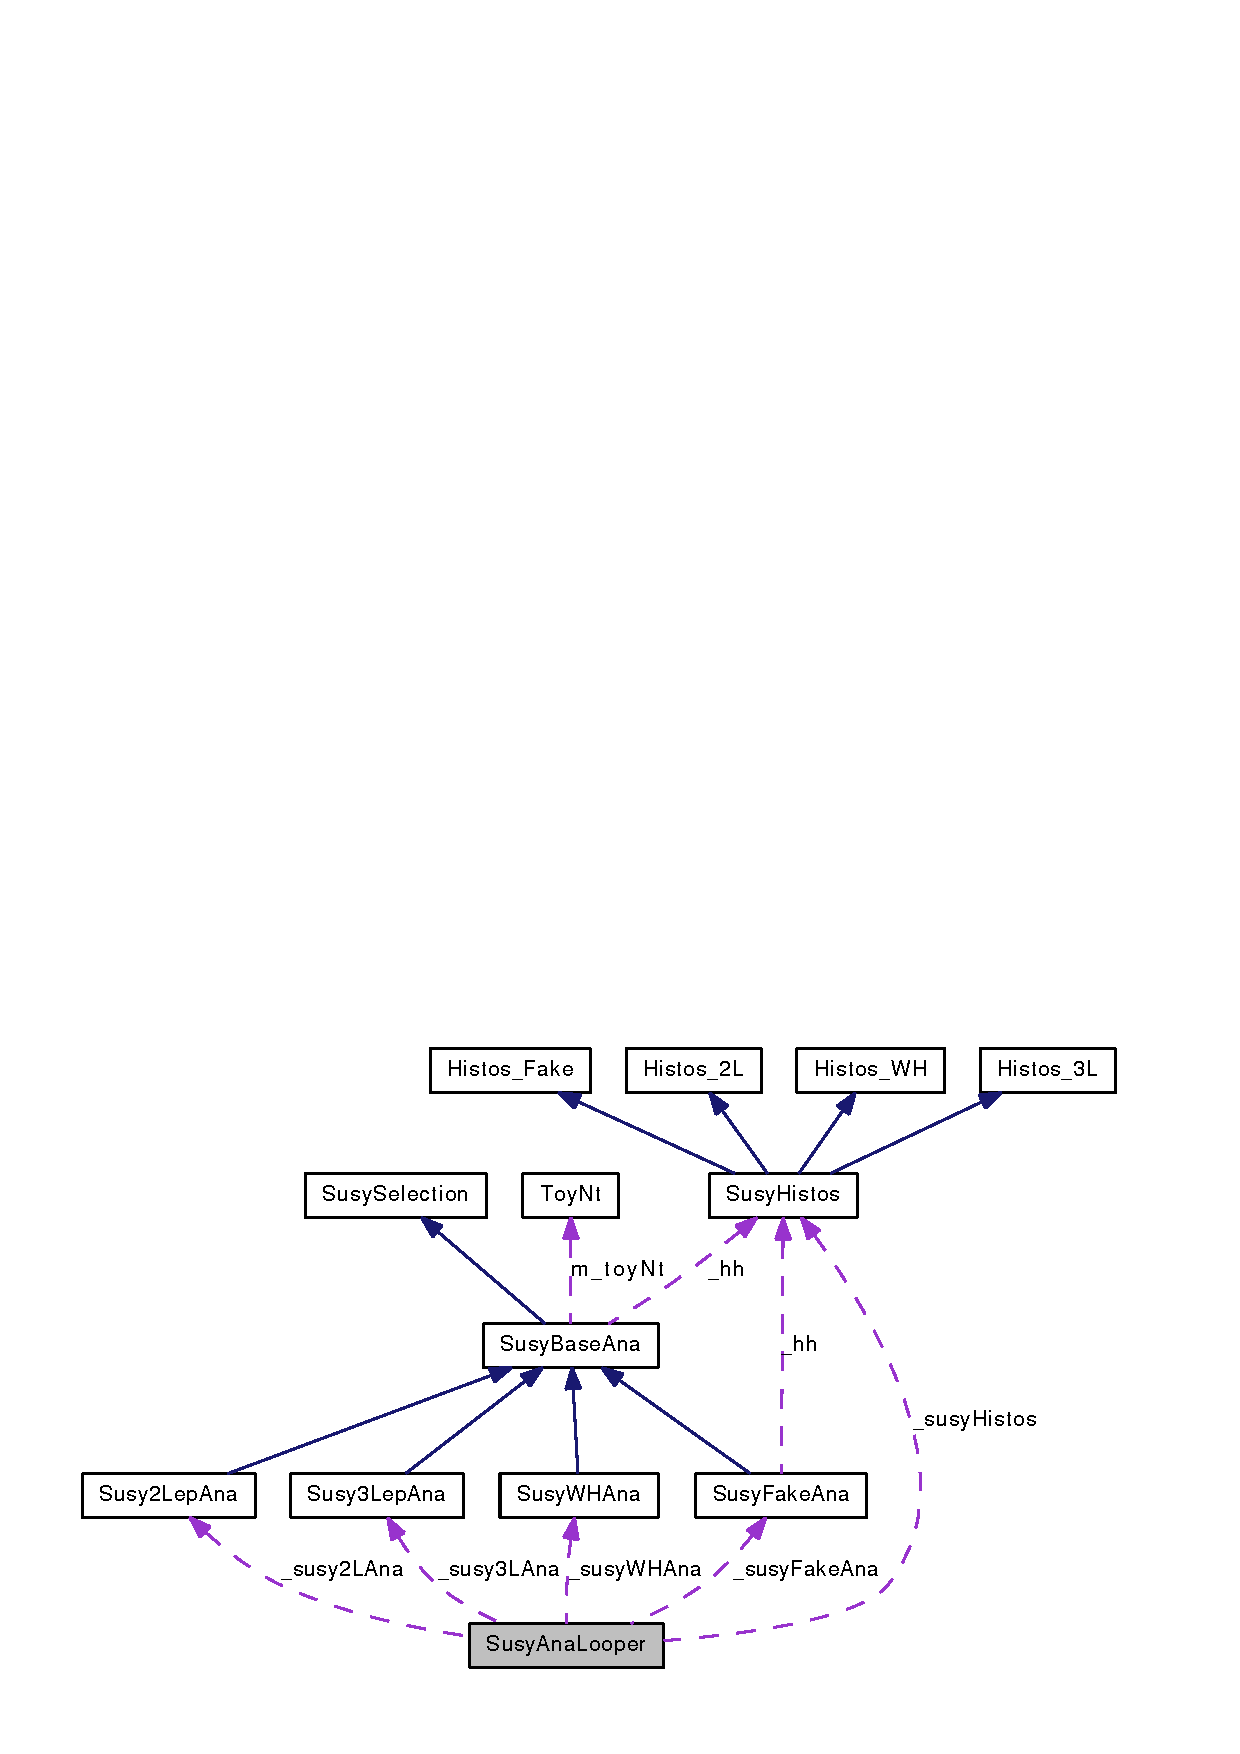
\includegraphics[width=400pt]{classSusyAnaLooper__coll__graph}
\end{center}
\end{figure}
\subsection*{Public Member Functions}
\begin{DoxyCompactItemize}
\item 
\hypertarget{classSusyAnaLooper_a62c8f06274c7c1e4e453ca18d236f522}{
{\bfseries SusyAnaLooper} (bool do2L, bool do3L, bool doWH, bool doFake)}
\label{classSusyAnaLooper_a62c8f06274c7c1e4e453ca18d236f522}

\item 
\hypertarget{classSusyAnaLooper_a37e438cc3d5d99c2b91ef1c19a68af75}{
virtual void {\bfseries Init} (TTree $\ast$tree)}
\label{classSusyAnaLooper_a37e438cc3d5d99c2b91ef1c19a68af75}

\item 
\hypertarget{classSusyAnaLooper_aae83c4cbdc242a5ee522f511d8db4499}{
virtual void {\bfseries Begin} (TTree $\ast$tree)}
\label{classSusyAnaLooper_aae83c4cbdc242a5ee522f511d8db4499}

\item 
\hypertarget{classSusyAnaLooper_a5d0f21b66aa21e2183dfcd8d17f78f6e}{
virtual void {\bfseries Terminate} ()}
\label{classSusyAnaLooper_a5d0f21b66aa21e2183dfcd8d17f78f6e}

\item 
\hypertarget{classSusyAnaLooper_a6ed3a9c898f025edceb668140a40936f}{
virtual Bool\_\-t {\bfseries Process} (Long64\_\-t entry)}
\label{classSusyAnaLooper_a6ed3a9c898f025edceb668140a40936f}

\item 
\hypertarget{classSusyAnaLooper_a1f21e974177b70f9145cffda05c8bd64}{
void {\bfseries setMCWeighter} (MCWeighter $\ast$mcw)}
\label{classSusyAnaLooper_a1f21e974177b70f9145cffda05c8bd64}

\item 
\hypertarget{classSusyAnaLooper_a74f1991be8d6afb842bc3e6636066ecc}{
void {\bfseries do2L} (bool b)}
\label{classSusyAnaLooper_a74f1991be8d6afb842bc3e6636066ecc}

\item 
\hypertarget{classSusyAnaLooper_afb7a243343611dd795d52d030a4f5615}{
void {\bfseries doWH} (bool b)}
\label{classSusyAnaLooper_afb7a243343611dd795d52d030a4f5615}

\item 
\hypertarget{classSusyAnaLooper_a68ac165ca3c057d74cdd56e0b5bc73eb}{
void {\bfseries doMll} (bool b)}
\label{classSusyAnaLooper_a68ac165ca3c057d74cdd56e0b5bc73eb}

\item 
\hypertarget{classSusyAnaLooper_ac052d906c31f6143c6c4a2cfec9c166d}{
void {\bfseries do3L} (bool b)}
\label{classSusyAnaLooper_ac052d906c31f6143c6c4a2cfec9c166d}

\item 
\hypertarget{classSusyAnaLooper_adb001d7df8be127ce626abb12f2d3735}{
void {\bfseries setMethod} (int m)}
\label{classSusyAnaLooper_adb001d7df8be127ce626abb12f2d3735}

\item 
\hypertarget{classSusyAnaLooper_aa65a103d4ad98c201fce242b612adba2}{
void {\bfseries setSystematic} (string sys)}
\label{classSusyAnaLooper_aa65a103d4ad98c201fce242b612adba2}

\item 
\hypertarget{classSusyAnaLooper_a2828279e51a904222ecfbcb9cfa51015}{
void {\bfseries doSysRange} (string sys1, string sys2)}
\label{classSusyAnaLooper_a2828279e51a904222ecfbcb9cfa51015}

\item 
\hypertarget{classSusyAnaLooper_a435f3dd21a498e30111946be71d75019}{
int {\bfseries getSysIndex} (string sys)}
\label{classSusyAnaLooper_a435f3dd21a498e30111946be71d75019}

\item 
\hypertarget{classSusyAnaLooper_aa1e947b5f0a2ac1022b81b5cfadfdc49}{
void {\bfseries useLooseLep} (bool b)}
\label{classSusyAnaLooper_aa1e947b5f0a2ac1022b81b5cfadfdc49}

\item 
\hypertarget{classSusyAnaLooper_affd68ac0284639f1234a94cc8fbc3b7f}{
void {\bfseries printSettings} ()}
\label{classSusyAnaLooper_affd68ac0284639f1234a94cc8fbc3b7f}

\item 
\hypertarget{classSusyAnaLooper_a5863f5b3dae4cebe1ae59a93775c437f}{
void {\bfseries dumpEvent} ()}
\label{classSusyAnaLooper_a5863f5b3dae4cebe1ae59a93775c437f}

\item 
\hypertarget{classSusyAnaLooper_a59c8f810dee28ff07a0028d3e068068b}{
{\bfseries ClassDef} (\hyperlink{classSusyAnaLooper}{SusyAnaLooper}, 1)}
\label{classSusyAnaLooper_a59c8f810dee28ff07a0028d3e068068b}

\end{DoxyCompactItemize}
\subsection*{Public Attributes}
\begin{DoxyCompactItemize}
\item 
\hypertarget{classSusyAnaLooper_a52c42bb8b5d505421099cb512bb32520}{
ofstream {\bfseries out}}
\label{classSusyAnaLooper_a52c42bb8b5d505421099cb512bb32520}

\end{DoxyCompactItemize}
\subsection*{Protected Attributes}
\begin{DoxyCompactItemize}
\item 
\hypertarget{classSusyAnaLooper_a0528b9decc0697efc1de4ecf7bc83c72}{
TDirectory $\ast$ {\bfseries \_\-histoDir}}
\label{classSusyAnaLooper_a0528b9decc0697efc1de4ecf7bc83c72}

\item 
\hypertarget{classSusyAnaLooper_ab4e0f2f266af4df3396ef13e4812938b}{
\hyperlink{classSusyHistos}{SusyHistos} $\ast$ {\bfseries \_\-susyHistos}}
\label{classSusyAnaLooper_ab4e0f2f266af4df3396ef13e4812938b}

\item 
\hypertarget{classSusyAnaLooper_a8ca252a368fb98e824050402c415cdba}{
\hyperlink{classSusy2LepAna}{Susy2LepAna} $\ast$ {\bfseries \_\-susy2LAna}}
\label{classSusyAnaLooper_a8ca252a368fb98e824050402c415cdba}

\item 
\hypertarget{classSusyAnaLooper_a7d9f3642f3694156d40b9a51dbf3772f}{
\hyperlink{classSusyWHAna}{SusyWHAna} $\ast$ {\bfseries \_\-susyWHAna}}
\label{classSusyAnaLooper_a7d9f3642f3694156d40b9a51dbf3772f}

\item 
\hypertarget{classSusyAnaLooper_a0b08135af98401f39f0b305ee6fcfae8}{
\hyperlink{classSusy3LepAna}{Susy3LepAna} $\ast$ {\bfseries \_\-susy3LAna}}
\label{classSusyAnaLooper_a0b08135af98401f39f0b305ee6fcfae8}

\item 
\hypertarget{classSusyAnaLooper_a177d49f68b3d9e8dfcaf4ac75646935f}{
\hyperlink{classSusyFakeAna}{SusyFakeAna} $\ast$ {\bfseries \_\-susyFakeAna}}
\label{classSusyAnaLooper_a177d49f68b3d9e8dfcaf4ac75646935f}

\item 
\hypertarget{classSusyAnaLooper_ae45366a275fd64f4dd1444713a648f3d}{
MCWeighter $\ast$ {\bfseries m\_\-mcWeighter}}
\label{classSusyAnaLooper_ae45366a275fd64f4dd1444713a648f3d}

\item 
\hypertarget{classSusyAnaLooper_a71d7ed4c4bc1b8f446777bf4271b2f27}{
bool {\bfseries \_\-do2LAna}}
\label{classSusyAnaLooper_a71d7ed4c4bc1b8f446777bf4271b2f27}

\item 
\hypertarget{classSusyAnaLooper_abb203285e2ed76de307db5048bb3e72a}{
bool {\bfseries \_\-doWHAna}}
\label{classSusyAnaLooper_abb203285e2ed76de307db5048bb3e72a}

\item 
\hypertarget{classSusyAnaLooper_a3637910408e476c7fe31aaffde968051}{
bool {\bfseries \_\-doMll}}
\label{classSusyAnaLooper_a3637910408e476c7fe31aaffde968051}

\item 
\hypertarget{classSusyAnaLooper_a61e38a93167d95eddc5f7264d3434392}{
bool {\bfseries \_\-do3LAna}}
\label{classSusyAnaLooper_a61e38a93167d95eddc5f7264d3434392}

\item 
\hypertarget{classSusyAnaLooper_ad4b5feb17de5aa42beee87ed11d55f4a}{
bool {\bfseries \_\-doFakeAna}}
\label{classSusyAnaLooper_ad4b5feb17de5aa42beee87ed11d55f4a}

\item 
\hypertarget{classSusyAnaLooper_abd7f5f7b9bd28a31c84d19df8c8867cd}{
bool {\bfseries \_\-useLooseLep}}
\label{classSusyAnaLooper_abd7f5f7b9bd28a31c84d19df8c8867cd}

\item 
\hypertarget{classSusyAnaLooper_ae904d97e8dc4eb3f570d4a66aa254579}{
int {\bfseries \_\-method}}
\label{classSusyAnaLooper_ae904d97e8dc4eb3f570d4a66aa254579}

\item 
\hypertarget{classSusyAnaLooper_a04596315fc5cb71d0b092e2aebaa2d00}{
string {\bfseries \_\-systematic1}}
\label{classSusyAnaLooper_a04596315fc5cb71d0b092e2aebaa2d00}

\item 
\hypertarget{classSusyAnaLooper_a315c36d8de239382f1b0f82ef2f06080}{
string {\bfseries \_\-systematic2}}
\label{classSusyAnaLooper_a315c36d8de239382f1b0f82ef2f06080}

\item 
\hypertarget{classSusyAnaLooper_a8537a1bce47f9727fd7cf4d453805d17}{
bool {\bfseries \_\-runOneSys}}
\label{classSusyAnaLooper_a8537a1bce47f9727fd7cf4d453805d17}

\item 
\hypertarget{classSusyAnaLooper_af60f64ae933a9dca8c803493997c0297}{
bool {\bfseries \_\-runSysRange}}
\label{classSusyAnaLooper_af60f64ae933a9dca8c803493997c0297}

\item 
\hypertarget{classSusyAnaLooper_acd9d5ac728222bda4b741678803b63b0}{
bool {\bfseries \_\-isZAlpgenSherpa}}
\label{classSusyAnaLooper_acd9d5ac728222bda4b741678803b63b0}

\item 
\hypertarget{classSusyAnaLooper_ae03bfb0a1cdb54d7fea1f06bdb9aaa92}{
int {\bfseries nHFOR}}
\label{classSusyAnaLooper_ae03bfb0a1cdb54d7fea1f06bdb9aaa92}

\item 
\hypertarget{classSusyAnaLooper_a398f656d353963ca38763265b292526f}{
int {\bfseries nMllCut}}
\label{classSusyAnaLooper_a398f656d353963ca38763265b292526f}

\end{DoxyCompactItemize}


The documentation for this class was generated from the following files:\begin{DoxyCompactItemize}
\item 
SusyWeakProdAna/SusyAnaLooper.h\item 
Root/SusyAnaLooper.cxx\end{DoxyCompactItemize}

\hypertarget{classSusyBaseAna}{
\section{SusyBaseAna Class Reference}
\label{classSusyBaseAna}\index{SusyBaseAna@{SusyBaseAna}}
}


Base class inherited by all analysis classes.  


{\ttfamily \#include $<$SusyBaseAna.h$>$}Inheritance diagram for SusyBaseAna:\nopagebreak
\begin{figure}[H]
\begin{center}
\leavevmode
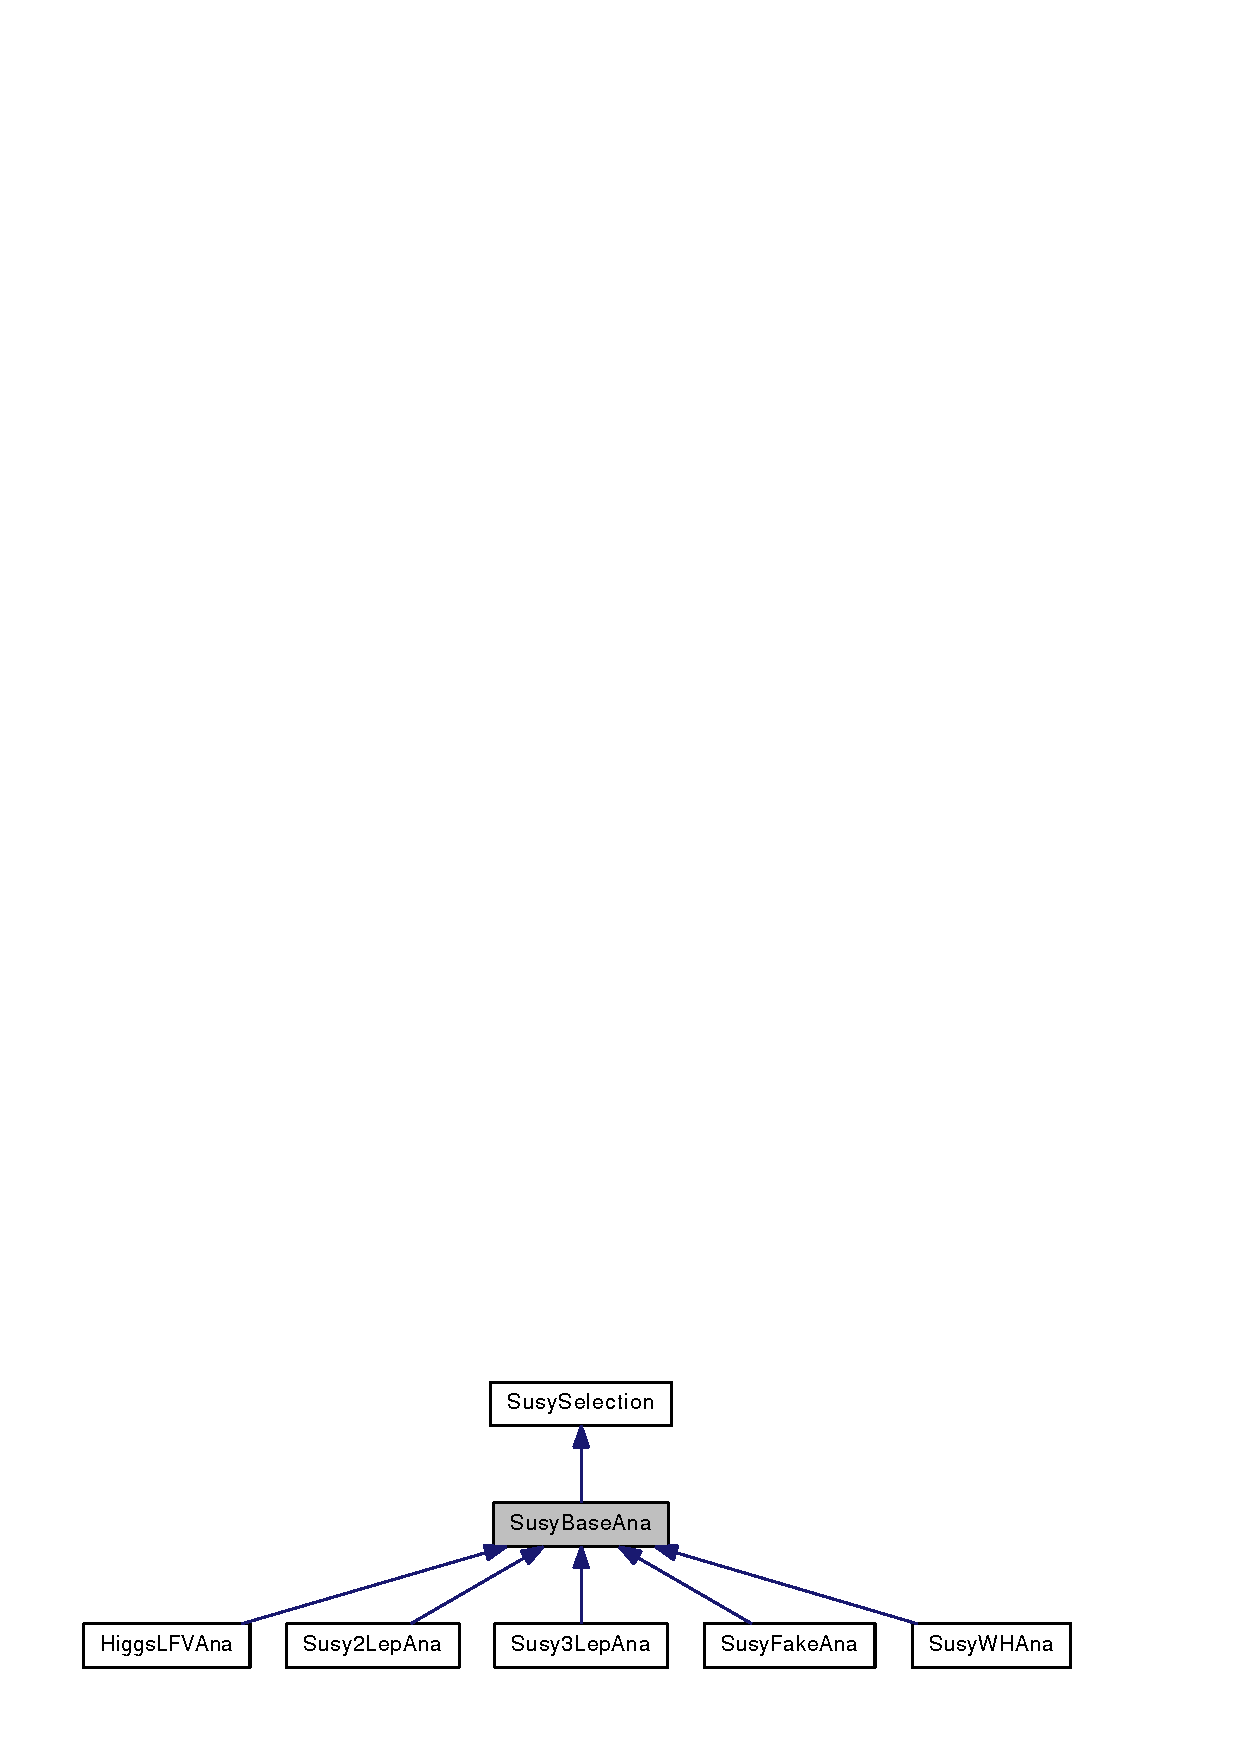
\includegraphics[width=400pt]{classSusyBaseAna__inherit__graph}
\end{center}
\end{figure}
Collaboration diagram for SusyBaseAna:\nopagebreak
\begin{figure}[H]
\begin{center}
\leavevmode
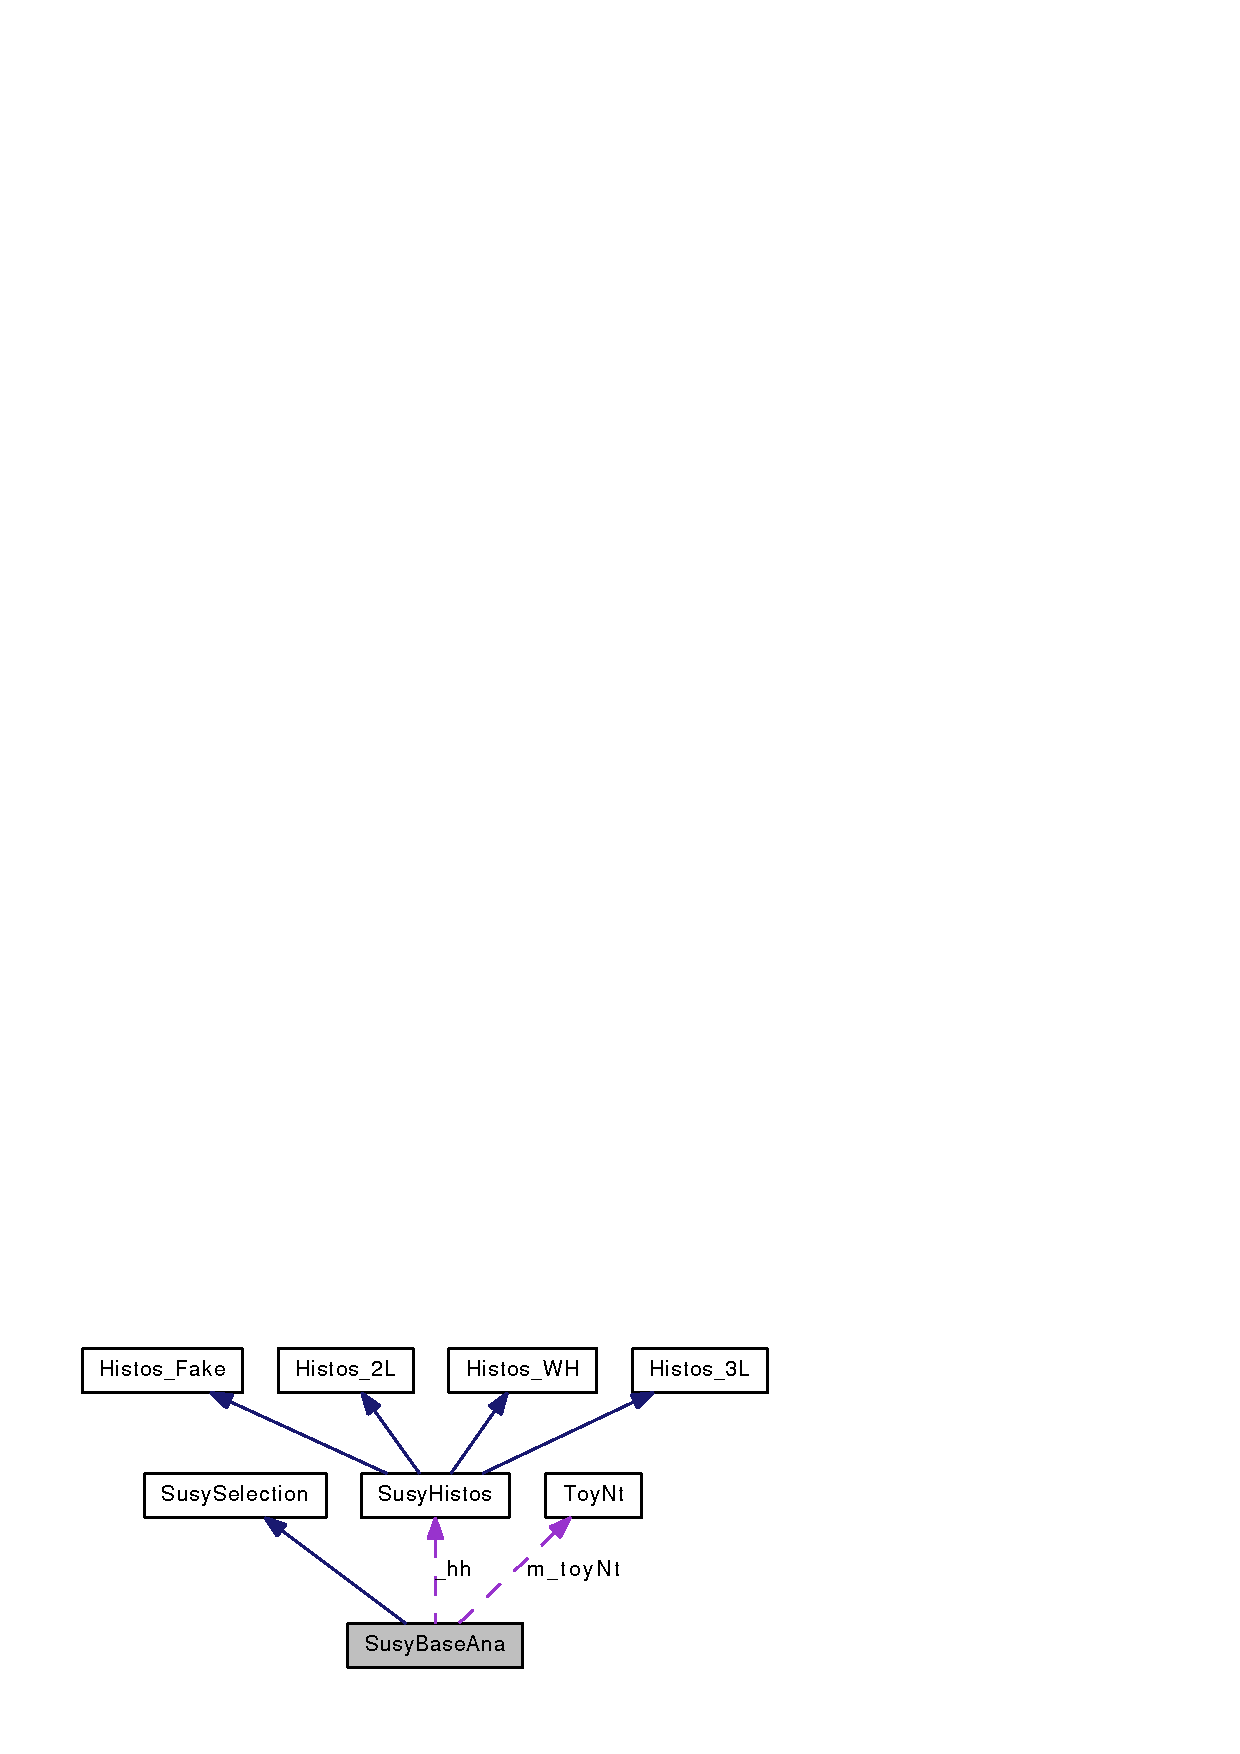
\includegraphics[width=372pt]{classSusyBaseAna__coll__graph}
\end{center}
\end{figure}
\subsection*{Public Member Functions}
\begin{DoxyCompactItemize}
\item 
\hypertarget{classSusyBaseAna_accf5ab460f9a98ff5caaea35218513ee}{
{\bfseries SusyBaseAna} (\hyperlink{classSusyHistos}{SusyHistos} $\ast$\_\-histos, bool is2LAna=true, bool isWHAna=false, bool qFlipd0=false)}
\label{classSusyBaseAna_accf5ab460f9a98ff5caaea35218513ee}

\item 
\hypertarget{classSusyBaseAna_a78e6d0b763df2f96ef0de1c2220e6a6a}{
void {\bfseries setUseLooseLep} (bool b)}
\label{classSusyBaseAna_a78e6d0b763df2f96ef0de1c2220e6a6a}

\item 
\hypertarget{classSusyBaseAna_a293ed2785910de12869f8b791d03788b}{
void {\bfseries setMethod} (int m)}
\label{classSusyBaseAna_a293ed2785910de12869f8b791d03788b}

\item 
\hypertarget{classSusyBaseAna_a9051f708fa685d0aac5edc6375d95344}{
void {\bfseries hookContainers} (Susy::SusyNtObject $\ast$\_\-ntPtr, ElectronVector $\ast$\_\-preEleA, ElectronVector $\ast$\_\-baseEleA, ElectronVector $\ast$\_\-sigEleA, MuonVector $\ast$\_\-preMuoA, MuonVector $\ast$\_\-baseMuoA, MuonVector $\ast$\_\-sigMuoA, LeptonVector $\ast$\_\-baseLepA, LeptonVector $\ast$\_\-sigLepA, JetVector $\ast$\_\-preJetA, JetVector $\ast$\_\-baseJetA, JetVector $\ast$\_\-sigJetA, TauVector $\ast$\_\-baseTauA, TauVector $\ast$\_\-sigTauA)}
\label{classSusyBaseAna_a9051f708fa685d0aac5edc6375d95344}

\item 
\hypertarget{classSusyBaseAna_ad8ec8c7886d0d265963f6744da7a6522}{
void {\bfseries hookMet} (const Susy::Met $\ast$\_\-met)}
\label{classSusyBaseAna_ad8ec8c7886d0d265963f6744da7a6522}

\item 
\hypertarget{classSusyBaseAna_a69619f7eeac5b97852bdb8e77b45a13a}{
bool {\bfseries isSimplifiedModelGrid} (int dsId)}
\label{classSusyBaseAna_a69619f7eeac5b97852bdb8e77b45a13a}

\item 
\hypertarget{classSusyBaseAna_ad7e0a457c025155b13d14f53cf57b777}{
float {\bfseries getXsUncert} (uint dsid)}
\label{classSusyBaseAna_ad7e0a457c025155b13d14f53cf57b777}

\item 
\hypertarget{classSusyBaseAna_aad612e1174deda592686352ffaa29bc3}{
float {\bfseries getLepSFWeight} (const LeptonVector $\ast$leptons, uint iSys=DGSys\_\-NOM)}
\label{classSusyBaseAna_aad612e1174deda592686352ffaa29bc3}

\item 
\hypertarget{classSusyBaseAna_a92a852f309b7fbd33468f2a5f83c787f}{
float {\bfseries getTriggerWeight} (const LeptonVector $\ast$leptons, float met, int nSignalJets, int npv, uint iSys=DGSys\_\-NOM)}
\label{classSusyBaseAna_a92a852f309b7fbd33468f2a5f83c787f}

\item 
\hypertarget{classSusyBaseAna_a65224353aae95449d5b6dd790d9f1768}{
float {\bfseries getBTagSF} (const Susy::Event $\ast$, const JetVector $\ast$jets, uint iSys=DGSys\_\-NOM)}
\label{classSusyBaseAna_a65224353aae95449d5b6dd790d9f1768}

\item 
\hypertarget{classSusyBaseAna_a49853feb82dbd4a1ef9a012c2bbf58e5}{
void {\bfseries finish} ()}
\label{classSusyBaseAna_a49853feb82dbd4a1ef9a012c2bbf58e5}

\item 
\hypertarget{classSusyBaseAna_a275dcbcfe10ff6cbdee5dd2217ae8995}{
void {\bfseries print\_\-line} (string s, float a, float b, float c)}
\label{classSusyBaseAna_a275dcbcfe10ff6cbdee5dd2217ae8995}

\item 
\hypertarget{classSusyBaseAna_a7264ac8641bb1592be5be230c0b5e099}{
void {\bfseries print\_\-line} (string s, int istart, int iend, float array\mbox{[}LEP\_\-N\mbox{]})}
\label{classSusyBaseAna_a7264ac8641bb1592be5be230c0b5e099}

\item 
\hypertarget{classSusyBaseAna_ae3eb899634929fe37035f00bec252e02}{
void {\bfseries print\_\-line} (string s, int istart, int iend, int sr, float array\mbox{[}LEP\_\-N\mbox{]}\mbox{[}SR\_\-N\mbox{]})}
\label{classSusyBaseAna_ae3eb899634929fe37035f00bec252e02}

\item 
\hypertarget{classSusyBaseAna_acf83b46b750b0832b43cedbb09c9529e}{
void {\bfseries saveOriginal} ()}
\label{classSusyBaseAna_acf83b46b750b0832b43cedbb09c9529e}

\item 
\hypertarget{classSusyBaseAna_a8428b73112a64359f58791c557ee3f63}{
void {\bfseries restoreOriginal} (LeptonVector \&leptons, const Met $\ast$met)}
\label{classSusyBaseAna_a8428b73112a64359f58791c557ee3f63}

\item 
\hypertarget{classSusyBaseAna_add60fe54c904c946639aa129b12d48b5}{
void {\bfseries clearVectors} ()}
\label{classSusyBaseAna_add60fe54c904c946639aa129b12d48b5}

\item 
\hypertarget{classSusyBaseAna_a77b45dc84d04140ac293aee3b5012745}{
void {\bfseries setMcSysMinMax} (uint sys1=DGSys\_\-NOM, uint sys2=DGSys\_\-Pileup\_\-DN)}
\label{classSusyBaseAna_a77b45dc84d04140ac293aee3b5012745}

\item 
\hypertarget{classSusyBaseAna_a7167e1ce20469860098d8a593400901e}{
void {\bfseries initializeToyNt} (bool metD=false, bool dijetB=false, bool OS2LB=false, bool SS2LB=false, bool ZBalB=false, bool diverVarsB=false, bool fakeB=false)}
\label{classSusyBaseAna_a7167e1ce20469860098d8a593400901e}

\item 
\hypertarget{classSusyBaseAna_a9acbfd9acb5d7b6f2ec899ad005b9786}{
void {\bfseries fillToyNt} (uint iSYS, const LeptonVector $\ast$leptons, const JetVector $\ast$jets, const Met $\ast$met, float \_\-ww, float \_\-wwBTag, float \_\-wwQFlip)}
\label{classSusyBaseAna_a9acbfd9acb5d7b6f2ec899ad005b9786}

\item 
\hypertarget{classSusyBaseAna_a6f6a198f8cc0f7b295caa7ca981bece7}{
void {\bfseries dumpEvent} ()}
\label{classSusyBaseAna_a6f6a198f8cc0f7b295caa7ca981bece7}

\item 
\hypertarget{classSusyBaseAna_a64cb7644fc15d4342013d9c313f940eb}{
void {\bfseries dumpLeptons} (const LeptonVector $\ast$leptons)}
\label{classSusyBaseAna_a64cb7644fc15d4342013d9c313f940eb}

\item 
\hypertarget{classSusyBaseAna_ac74908d780e64ea0ae016d87d1a2ff65}{
void {\bfseries dumpJets} (const JetVector $\ast$jets)}
\label{classSusyBaseAna_ac74908d780e64ea0ae016d87d1a2ff65}

\item 
\hypertarget{classSusyBaseAna_a110acd130bf5ee0b7ed2f74a9ed949d9}{
void {\bfseries dumpTrigger} ()}
\label{classSusyBaseAna_a110acd130bf5ee0b7ed2f74a9ed949d9}

\item 
\hypertarget{classSusyBaseAna_a5579c2261e2f72d0c753361273e9b579}{
{\bfseries ClassDef} (\hyperlink{classSusyBaseAna}{SusyBaseAna}, 1)}
\label{classSusyBaseAna_a5579c2261e2f72d0c753361273e9b579}

\end{DoxyCompactItemize}
\subsection*{Protected Attributes}
\begin{DoxyCompactItemize}
\item 
\hypertarget{classSusyBaseAna_a367bd65db63346df07ddd580294af668}{
\hyperlink{classSusyHistos}{SusyHistos} $\ast$ {\bfseries \_\-hh}}
\label{classSusyBaseAna_a367bd65db63346df07ddd580294af668}

\item 
\hypertarget{classSusyBaseAna_a442fc5acd64350b7af670237a3caa2bd}{
\hyperlink{classToyNt}{ToyNt} $\ast$ {\bfseries m\_\-toyNt}}
\label{classSusyBaseAna_a442fc5acd64350b7af670237a3caa2bd}

\item 
\hypertarget{classSusyBaseAna_a222bf62a46a03eebda35c795d0e1f46b}{
DilTrigLogic $\ast$ {\bfseries m\_\-trigObj}}
\label{classSusyBaseAna_a222bf62a46a03eebda35c795d0e1f46b}

\item 
\hypertarget{classSusyBaseAna_ae93079dc51825393f6c3f70759a03f2d}{
TrilTrigLogic $\ast$ {\bfseries m\_\-trig3LObj}}
\label{classSusyBaseAna_ae93079dc51825393f6c3f70759a03f2d}

\item 
\hypertarget{classSusyBaseAna_ae5de4586a5d7d2eb20f1ad4ce8ed87d6}{
SusyMatrixMethod::DiLeptonMatrixMethod {\bfseries m\_\-matrix\_\-method}}
\label{classSusyBaseAna_ae5de4586a5d7d2eb20f1ad4ce8ed87d6}

\item 
\hypertarget{classSusyBaseAna_ac1177a441f9e79e014cc936c98e9dca9}{
SameSignMatrixMethod::DiLeptonMatrixMethod {\bfseries m\_\-matrix\_\-methodWH}}
\label{classSusyBaseAna_ac1177a441f9e79e014cc936c98e9dca9}

\item 
\hypertarget{classSusyBaseAna_a7c2b27602fc8ca489a91a8a679c427ce}{
bool {\bfseries m\_\-useLooseLep}}
\label{classSusyBaseAna_a7c2b27602fc8ca489a91a8a679c427ce}

\item 
\hypertarget{classSusyBaseAna_a8655efab2d0fe20e78ce15b78ad53e67}{
int {\bfseries m\_\-method}}
\label{classSusyBaseAna_a8655efab2d0fe20e78ce15b78ad53e67}

\item 
\hypertarget{classSusyBaseAna_a2e19b9c79b7cee0f7940cf0e70297fe6}{
bool {\bfseries m\_\-writeToyNt}}
\label{classSusyBaseAna_a2e19b9c79b7cee0f7940cf0e70297fe6}

\item 
\hypertarget{classSusyBaseAna_a964237851f19aa3e9804fab95f71688f}{
uint {\bfseries \_\-sys1}}
\label{classSusyBaseAna_a964237851f19aa3e9804fab95f71688f}

\item 
\hypertarget{classSusyBaseAna_a5f1448f8ab04639816ab6c0f199fca5e}{
uint {\bfseries \_\-sys2}}
\label{classSusyBaseAna_a5f1448f8ab04639816ab6c0f199fca5e}

\item 
\hypertarget{classSusyBaseAna_adeadb0175b1d269ac471adfb4308ee80}{
XSReader $\ast$ {\bfseries susyXS}}
\label{classSusyBaseAna_adeadb0175b1d269ac471adfb4308ee80}

\item 
\hypertarget{classSusyBaseAna_a4a3f6e6a46a87dc92765a5b30a460781}{
ofstream {\bfseries out}}
\label{classSusyBaseAna_a4a3f6e6a46a87dc92765a5b30a460781}

\item 
\hypertarget{classSusyBaseAna_a442fe2a2c2bd557a54f1aecf3c8d7147}{
ofstream {\bfseries evtDump}}
\label{classSusyBaseAna_a442fe2a2c2bd557a54f1aecf3c8d7147}

\item 
\hypertarget{classSusyBaseAna_a2532294a1f669a773730d8a89ac95335}{
ifstream {\bfseries sigXsfile}}
\label{classSusyBaseAna_a2532294a1f669a773730d8a89ac95335}

\end{DoxyCompactItemize}


\subsection{Detailed Description}
Base class inherited by all analysis classes. Contains common functions used by all analysis code. 

The documentation for this class was generated from the following files:\begin{DoxyCompactItemize}
\item 
SusyWeakProdAna/SusyBaseAna.h\item 
Root/SusyBaseAna.cxx\end{DoxyCompactItemize}

\hypertarget{classSusyFakeAna}{
\section{SusyFakeAna Class Reference}
\label{classSusyFakeAna}\index{SusyFakeAna@{SusyFakeAna}}
}
Inheritance diagram for SusyFakeAna:\nopagebreak
\begin{figure}[H]
\begin{center}
\leavevmode
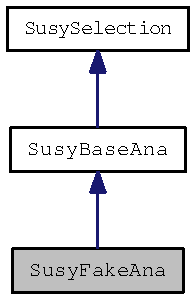
\includegraphics[width=130pt]{classSusyFakeAna__inherit__graph}
\end{center}
\end{figure}
Collaboration diagram for SusyFakeAna:\nopagebreak
\begin{figure}[H]
\begin{center}
\leavevmode
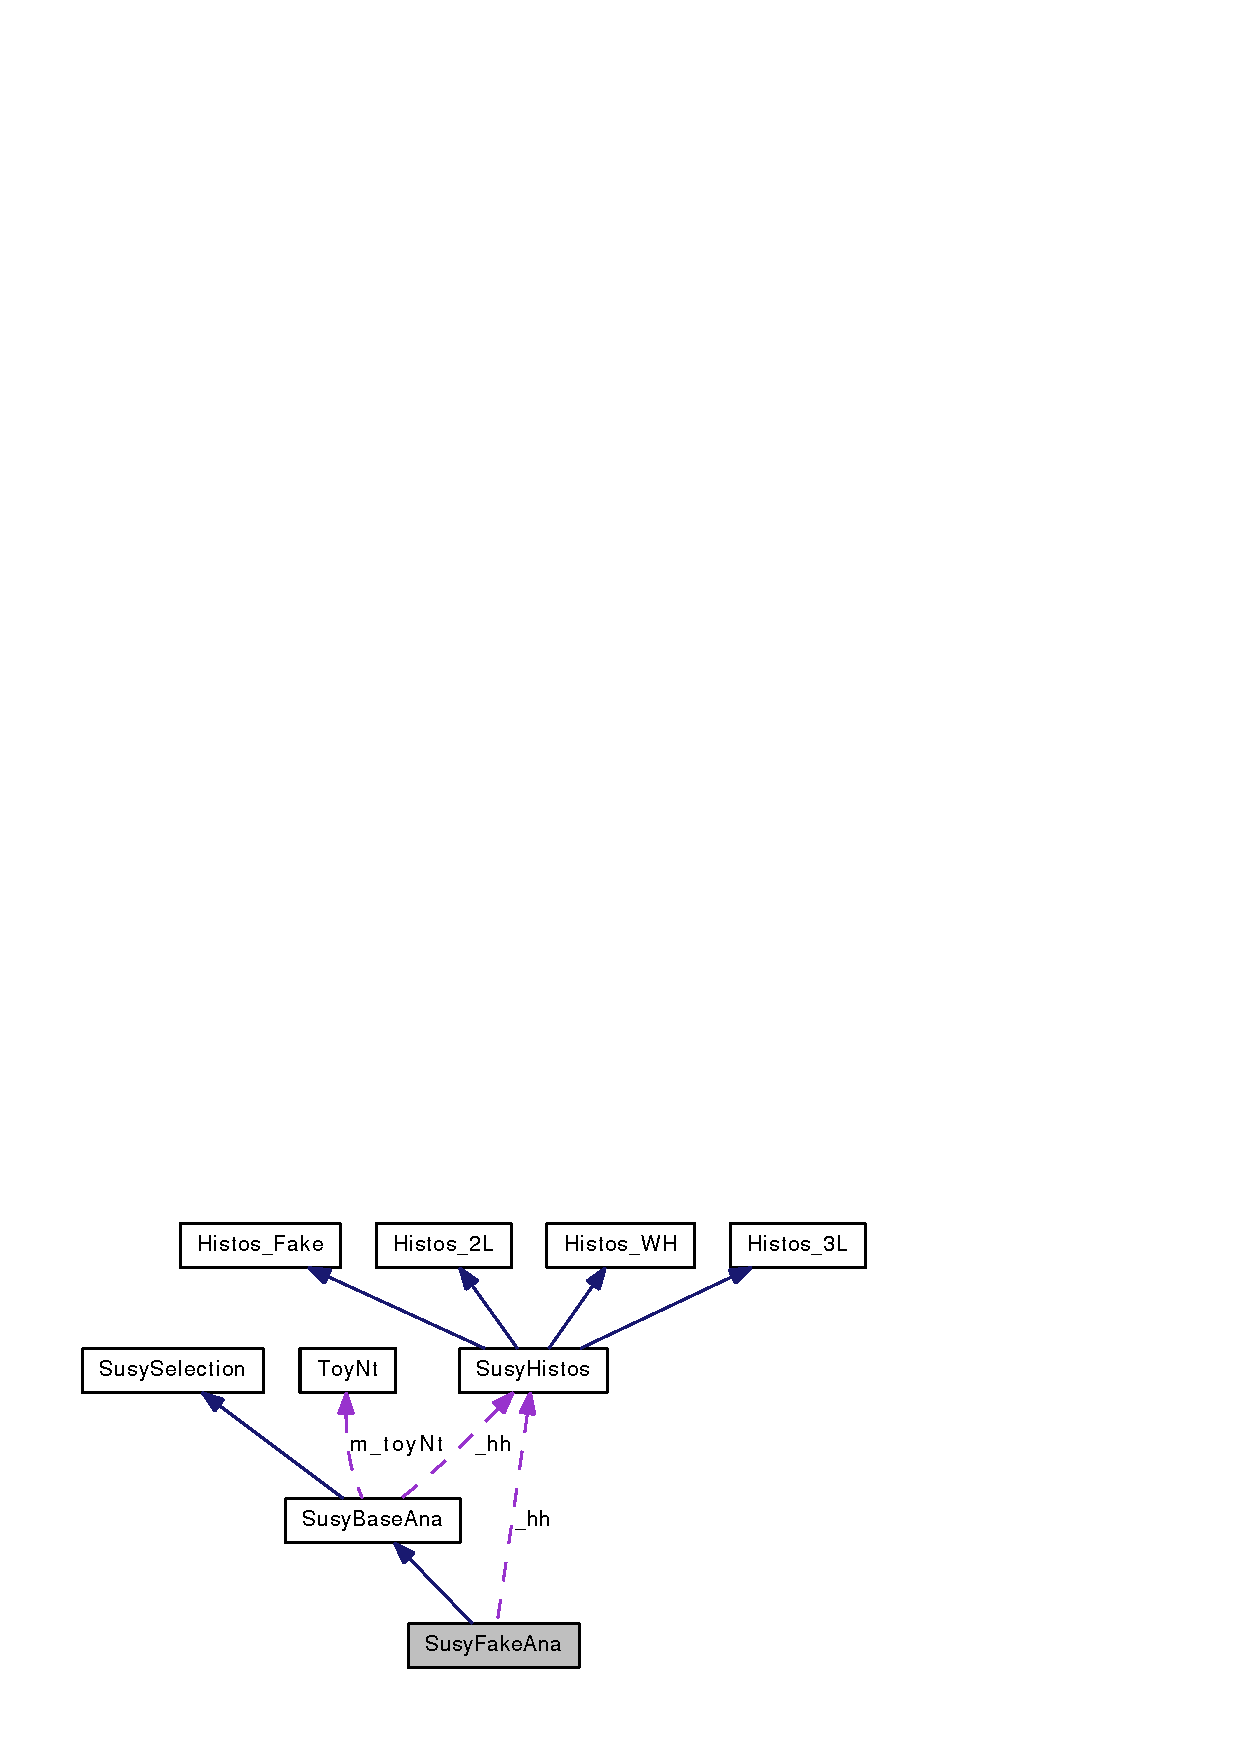
\includegraphics[width=400pt]{classSusyFakeAna__coll__graph}
\end{center}
\end{figure}
\subsection*{Public Member Functions}
\begin{DoxyCompactItemize}
\item 
\hypertarget{classSusyFakeAna_ac092fb9efc326ae084d888501bdfa818}{
{\bfseries SusyFakeAna} (\hyperlink{classSusyHistos}{SusyHistos} $\ast$\_\-histos)}
\label{classSusyFakeAna_ac092fb9efc326ae084d888501bdfa818}

\item 
\hypertarget{classSusyFakeAna_a28b10622b8d67eacee73cf2e1999903f}{
void {\bfseries doAnalysis} (float w, unsigned int isys=DGSys\_\-NOM)}
\label{classSusyFakeAna_a28b10622b8d67eacee73cf2e1999903f}

\item 
\hypertarget{classSusyFakeAna_a6b73ce1990391a6b0c56f866f7212d47}{
void {\bfseries end} ()}
\label{classSusyFakeAna_a6b73ce1990391a6b0c56f866f7212d47}

\item 
\hypertarget{classSusyFakeAna_a78bf4f98f92485fa76342ec8b2d628c7}{
bool {\bfseries selectEvent} (LeptonVector $\ast$baseLeptons, LeptonVector $\ast$signalLeptons, const JetVector $\ast$jets, const Met $\ast$met, float w)}
\label{classSusyFakeAna_a78bf4f98f92485fa76342ec8b2d628c7}

\item 
\hypertarget{classSusyFakeAna_aadf34572b99c75663a542a95b65b8539}{
void {\bfseries getEventWeights} (float w, LeptonVector $\ast$leptons, const JetVector $\ast$jets, const Met $\ast$met)}
\label{classSusyFakeAna_aadf34572b99c75663a542a95b65b8539}

\item 
\hypertarget{classSusyFakeAna_ac10b9f9e353c44f69ffa1076c0350060}{
bool {\bfseries passSelections} (LeptonVector $\ast$baseLeptons, LeptonVector $\ast$leptons, const JetVector $\ast$jets, const Met $\ast$met)}
\label{classSusyFakeAna_ac10b9f9e353c44f69ffa1076c0350060}

\item 
\hypertarget{classSusyFakeAna_ab5e76910363fb5470554ae3b8f5f6028}{
bool {\bfseries passSS1j} (LeptonVector $\ast$leptons, const JetVector $\ast$jets, const Met $\ast$met)}
\label{classSusyFakeAna_ab5e76910363fb5470554ae3b8f5f6028}

\item 
\hypertarget{classSusyFakeAna_a8510cb05b385d9ce2e06c235d6695675}{
bool {\bfseries passSSEM} (LeptonVector $\ast$leptons, const JetVector $\ast$jets, const Met $\ast$met)}
\label{classSusyFakeAna_a8510cb05b385d9ce2e06c235d6695675}

\item 
\hypertarget{classSusyFakeAna_a1f57517c038bdff8c7d72382f6b1a4ef}{
bool {\bfseries passHFTagProbe} (LeptonVector $\ast$leptons, const JetVector $\ast$jets, const Met $\ast$met)}
\label{classSusyFakeAna_a1f57517c038bdff8c7d72382f6b1a4ef}

\item 
\hypertarget{classSusyFakeAna_a8291a6aa3456fbe47a871d8d73671f4b}{
bool {\bfseries passMCExtractionEff} (LeptonVector $\ast$leptons, const JetVector $\ast$jets, const Met $\ast$met)}
\label{classSusyFakeAna_a8291a6aa3456fbe47a871d8d73671f4b}

\item 
\hypertarget{classSusyFakeAna_a738e92eae29559931cd367864f4093ad}{
bool {\bfseries passZTagProbe} (LeptonVector $\ast$leptons, const JetVector $\ast$jets, const Met $\ast$met)}
\label{classSusyFakeAna_a738e92eae29559931cd367864f4093ad}

\item 
\hypertarget{classSusyFakeAna_acfa1a2eec99956376334bdf5d8b5c5f8}{
bool {\bfseries passConv} (LeptonVector $\ast$leptons, const JetVector $\ast$jets, const Met $\ast$met)}
\label{classSusyFakeAna_acfa1a2eec99956376334bdf5d8b5c5f8}

\item 
\hypertarget{classSusyFakeAna_a5bf02cd10aef9593b878cc8650fec46d}{
bool {\bfseries passZHFLF} (LeptonVector $\ast$leptons, const JetVector $\ast$jets, const Met $\ast$met)}
\label{classSusyFakeAna_a5bf02cd10aef9593b878cc8650fec46d}

\item 
\hypertarget{classSusyFakeAna_a68866a94b43515c6cabfbe5cacf08b2c}{
{\bfseries ClassDef} (\hyperlink{classSusyFakeAna}{SusyFakeAna}, 1)}
\label{classSusyFakeAna_a68866a94b43515c6cabfbe5cacf08b2c}

\end{DoxyCompactItemize}
\subsection*{Protected Attributes}
\begin{DoxyCompactItemize}
\item 
\hypertarget{classSusyFakeAna_a74211b0988cd0d6e69384c7d5e7b501e}{
\hyperlink{classSusyHistos}{SusyHistos} $\ast$ {\bfseries \_\-hh}}
\label{classSusyFakeAna_a74211b0988cd0d6e69384c7d5e7b501e}

\item 
\hypertarget{classSusyFakeAna_aa7db2de4e8cc90a974d7bac6a83a8ea5}{
TRandom3 $\ast$ {\bfseries \_\-random}}
\label{classSusyFakeAna_aa7db2de4e8cc90a974d7bac6a83a8ea5}

\item 
\hypertarget{classSusyFakeAna_adebacecccd686d8eeda48628d39ad875}{
float {\bfseries \_\-ww}}
\label{classSusyFakeAna_adebacecccd686d8eeda48628d39ad875}

\item 
\hypertarget{classSusyFakeAna_acae786b13c0e22f62f30b8c0bfbcd499}{
float {\bfseries \_\-wwBck}}
\label{classSusyFakeAna_acae786b13c0e22f62f30b8c0bfbcd499}

\item 
\hypertarget{classSusyFakeAna_a77d5032ee788d9386daf27250ca98a02}{
float {\bfseries \_\-wwBTag}}
\label{classSusyFakeAna_a77d5032ee788d9386daf27250ca98a02}

\item 
\hypertarget{classSusyFakeAna_a442c949bcd2b7b24dc5d76386c1f8a25}{
float {\bfseries \_\-wwqFlip}}
\label{classSusyFakeAna_a442c949bcd2b7b24dc5d76386c1f8a25}

\item 
\hypertarget{classSusyFakeAna_a05c9ad1013c8ca5c12b4873e2880281a}{
int {\bfseries n\_\-pass\_\-SS1j}}
\label{classSusyFakeAna_a05c9ad1013c8ca5c12b4873e2880281a}

\item 
\hypertarget{classSusyFakeAna_abb428e8585b9e56cd65a6f47595155d7}{
int {\bfseries n\_\-pass\_\-SSEM}}
\label{classSusyFakeAna_abb428e8585b9e56cd65a6f47595155d7}

\item 
\hypertarget{classSusyFakeAna_a33b6bf19a8e416d4f9b203c85274423b}{
int {\bfseries n\_\-pass\_\-HFTagProbe}}
\label{classSusyFakeAna_a33b6bf19a8e416d4f9b203c85274423b}

\item 
\hypertarget{classSusyFakeAna_aa4b4d68942b6a7dd2006c6601d7e1d0a}{
int {\bfseries n\_\-pass\_\-MCExtractionEff}}
\label{classSusyFakeAna_aa4b4d68942b6a7dd2006c6601d7e1d0a}

\item 
\hypertarget{classSusyFakeAna_a95feee4f33f214554e29475b41c46051}{
int {\bfseries n\_\-pass\_\-ZTagProbe}}
\label{classSusyFakeAna_a95feee4f33f214554e29475b41c46051}

\item 
\hypertarget{classSusyFakeAna_ae203e2e952160c23b14aad4de6cca58f}{
int {\bfseries n\_\-pass\_\-ZConv}}
\label{classSusyFakeAna_ae203e2e952160c23b14aad4de6cca58f}

\item 
\hypertarget{classSusyFakeAna_a65fe91dac6ce7619f524cad7dfcd7854}{
int {\bfseries n\_\-pass\_\-ZHFLF}}
\label{classSusyFakeAna_a65fe91dac6ce7619f524cad7dfcd7854}

\end{DoxyCompactItemize}


The documentation for this class was generated from the following files:\begin{DoxyCompactItemize}
\item 
SusyWeakProdAna/SusyFakeAna.h\item 
Root/SusyFakeAna.cxx\end{DoxyCompactItemize}

\hypertarget{classSusyHistos}{
\section{SusyHistos Class Reference}
\label{classSusyHistos}\index{SusyHistos@{SusyHistos}}
}
Inheritance diagram for SusyHistos:\nopagebreak
\begin{figure}[H]
\begin{center}
\leavevmode
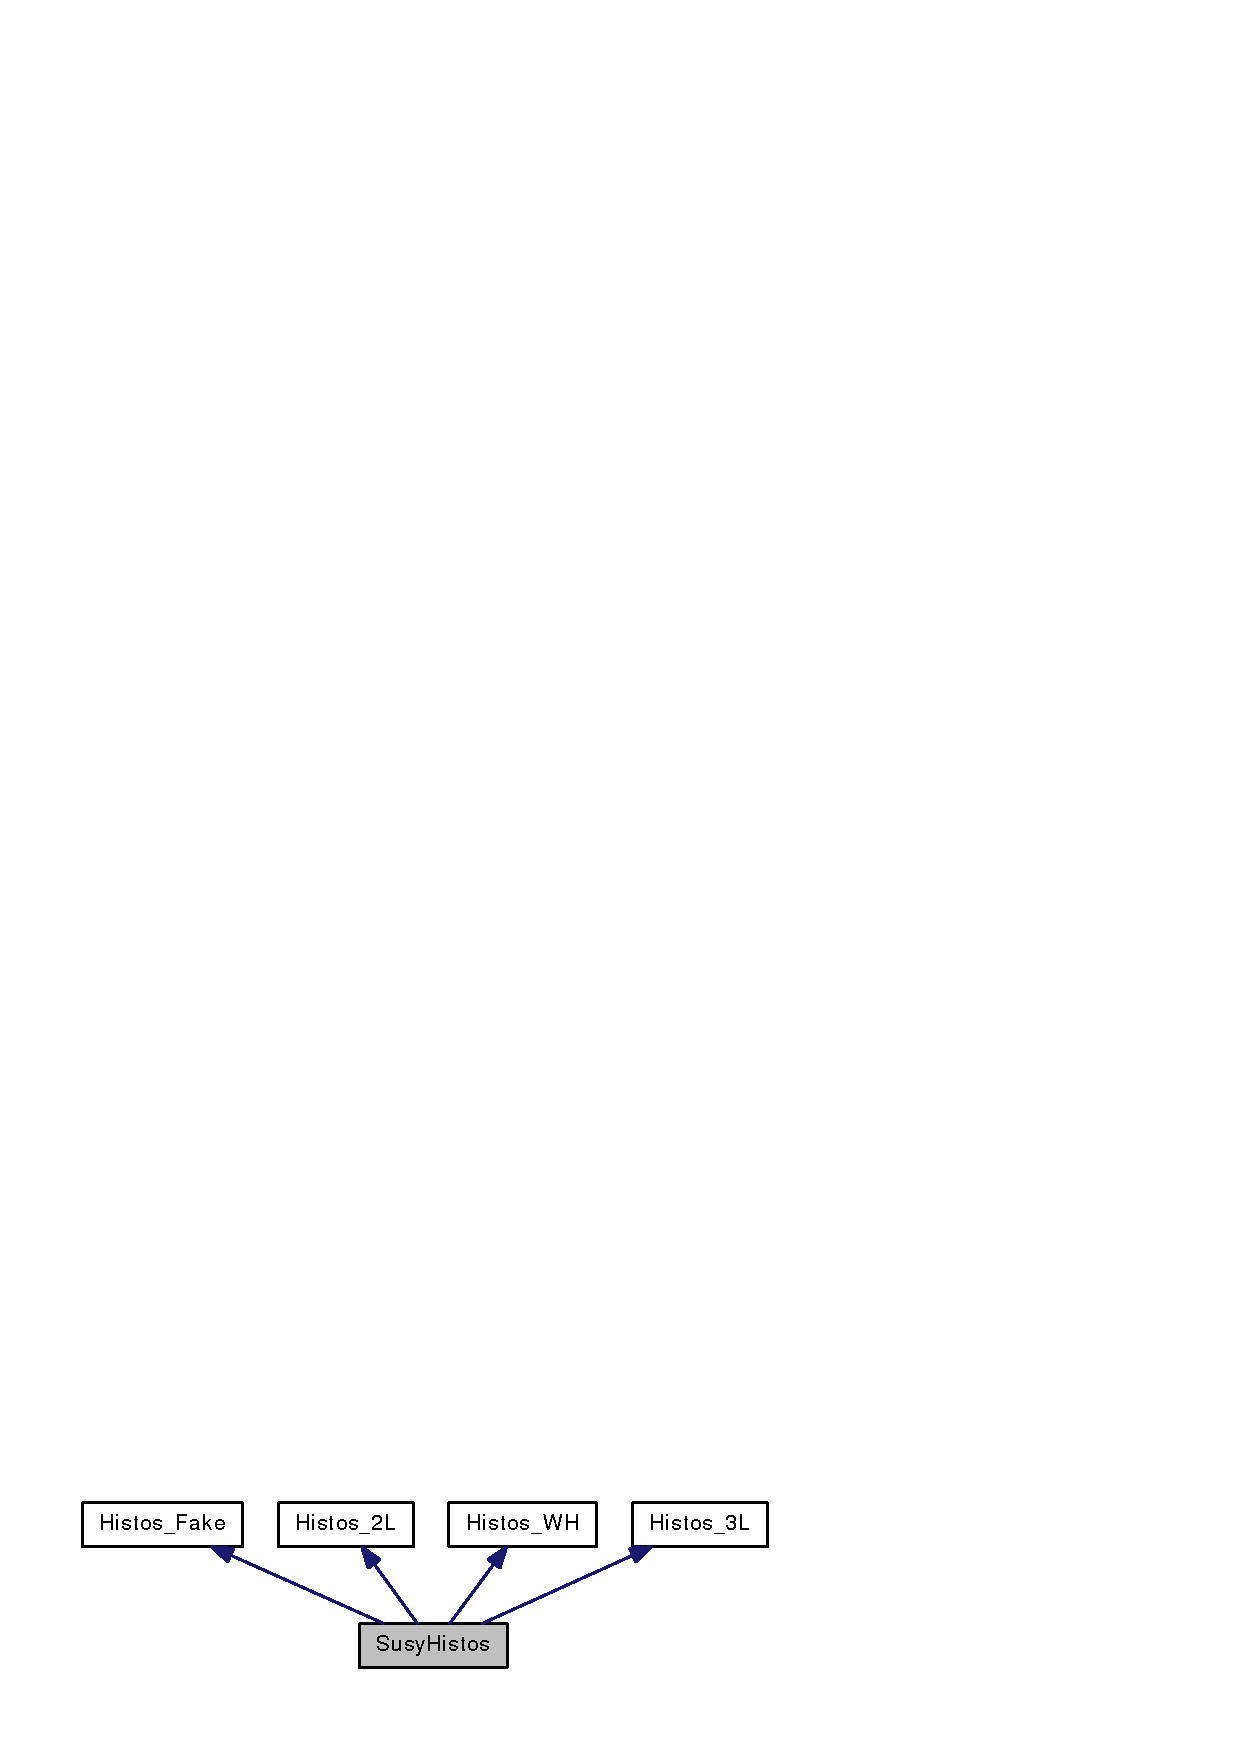
\includegraphics[width=372pt]{classSusyHistos__inherit__graph}
\end{center}
\end{figure}
Collaboration diagram for SusyHistos:\nopagebreak
\begin{figure}[H]
\begin{center}
\leavevmode
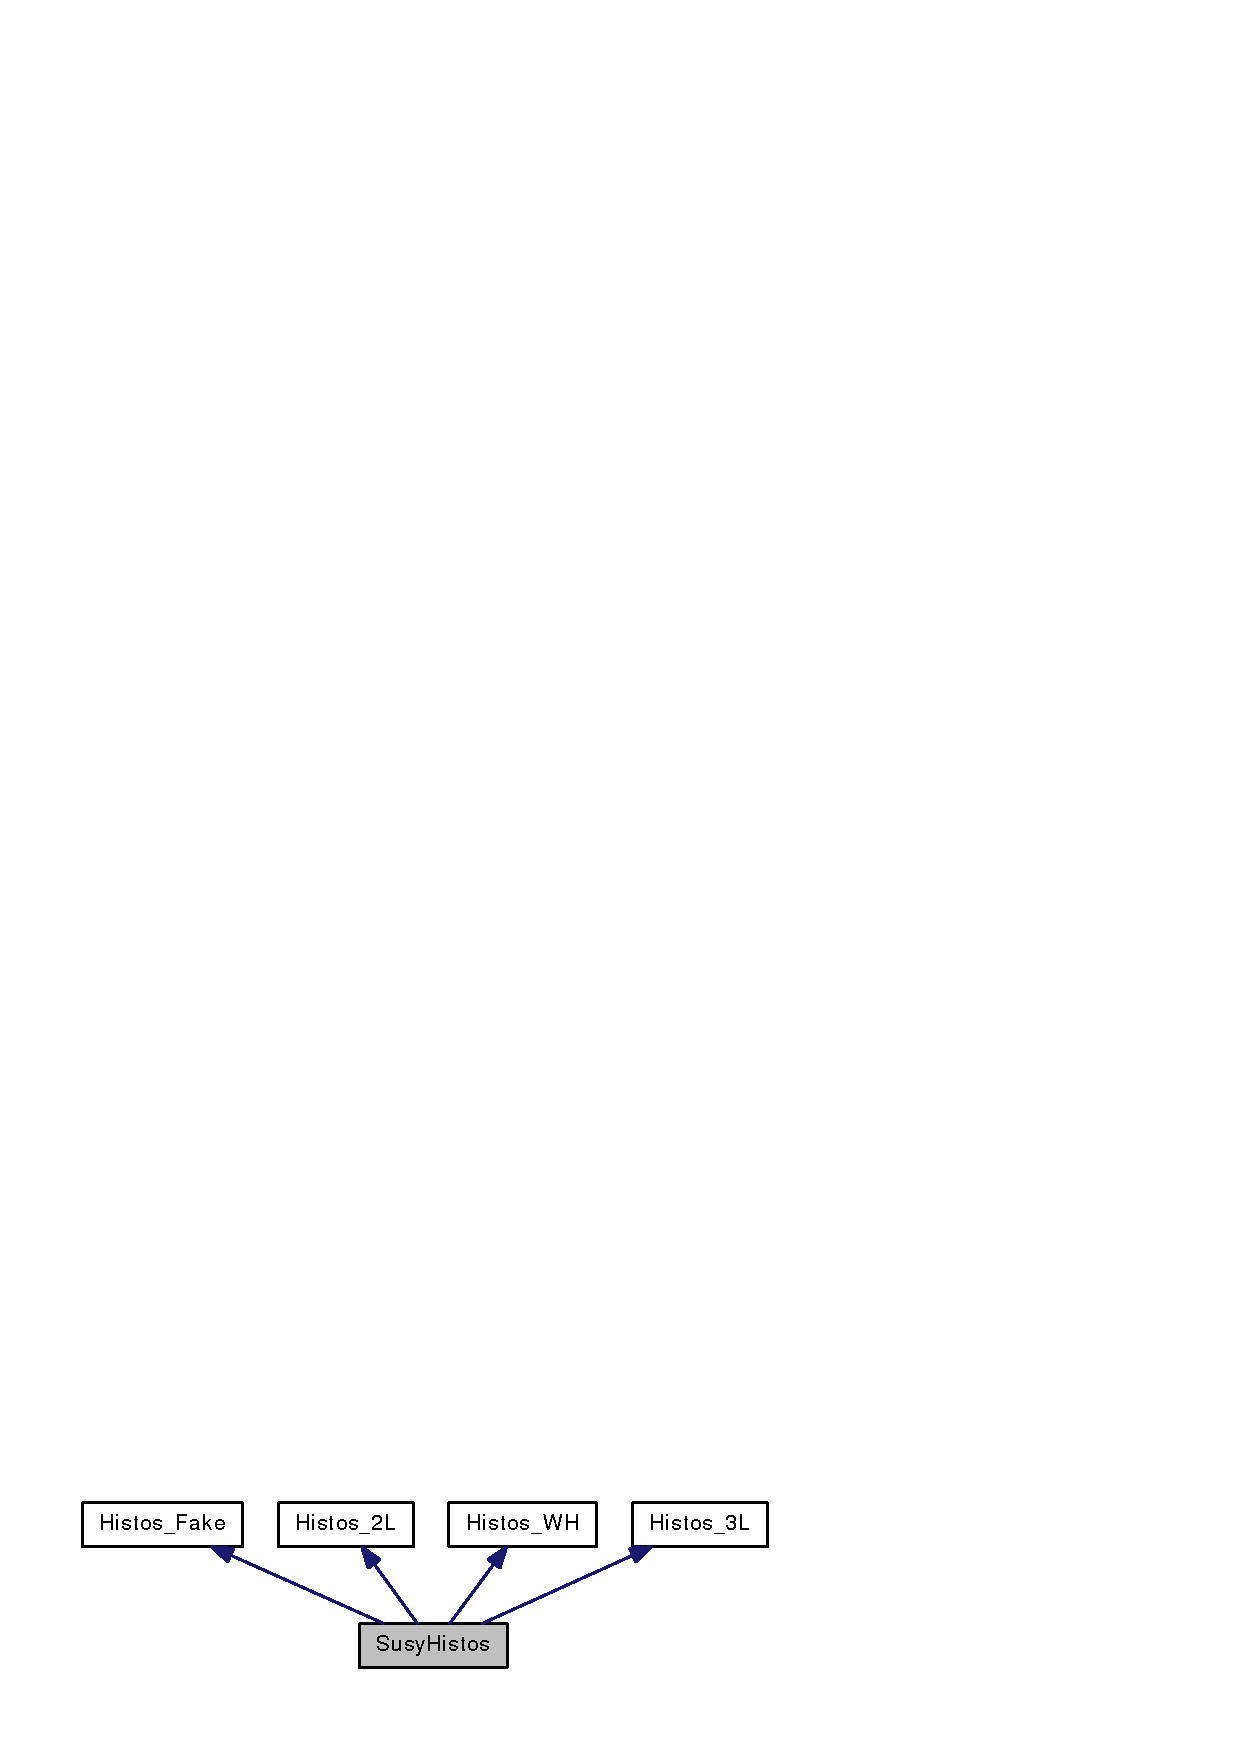
\includegraphics[width=372pt]{classSusyHistos__coll__graph}
\end{center}
\end{figure}
\subsection*{Public Member Functions}
\begin{DoxyCompactItemize}
\item 
\hypertarget{classSusyHistos_a7b988b4c8828c0dbfe376d908757a862}{
void {\bfseries setSample} (std::string s)}
\label{classSusyHistos_a7b988b4c8828c0dbfe376d908757a862}

\item 
\hypertarget{classSusyHistos_a28f9d44ef663c1efc1d976366de39c81}{
std::string {\bfseries sampleName} () const }
\label{classSusyHistos_a28f9d44ef663c1efc1d976366de39c81}

\item 
\hypertarget{classSusyHistos_a091d793996ecc86011fd875223f192ef}{
void {\bfseries SaveHistograms} (TDirectory $\ast$\_\-hDir, int method=STD, bool mcMll=false, bool isZAlpgenSherpa=false, string sys1=\char`\"{}\char`\"{}, string sys2=\char`\"{}\char`\"{})}
\label{classSusyHistos_a091d793996ecc86011fd875223f192ef}

\item 
\hypertarget{classSusyHistos_a14092bd49d755f07b3fb03d9a4e47149}{
void {\bfseries SaveSplit2LHistograms} (TDirectory $\ast$\_\-hDir, int method=STD, bool mcMll=false, bool isZAlpgenShepa=false, string sys1=\char`\"{}\char`\"{}, string sys2=\char`\"{}\char`\"{})}
\label{classSusyHistos_a14092bd49d755f07b3fb03d9a4e47149}

\item 
\hypertarget{classSusyHistos_a4e5a682cb040a60c91b92d3cf2a51c02}{
void {\bfseries SaveSplitWHHistograms} (TDirectory $\ast$\_\-hDir, int method=STD, bool mcMll=false, bool isZAlpgenShepa=false, string sys1=\char`\"{}\char`\"{}, string sys2=\char`\"{}\char`\"{})}
\label{classSusyHistos_a4e5a682cb040a60c91b92d3cf2a51c02}

\item 
\hypertarget{classSusyHistos_a597756bb5a013d3ca51a0fecb9a9744d}{
void {\bfseries SaveSplit3LHistograms} (TDirectory $\ast$\_\-hDir, int method=STD, bool mcMll=false, bool isZAlpgenShepa=false, string sys1=\char`\"{}\char`\"{}, string sys2=\char`\"{}\char`\"{})}
\label{classSusyHistos_a597756bb5a013d3ca51a0fecb9a9744d}

\item 
\hypertarget{classSusyHistos_a99c39fa0439e5be3b608de6b747366ef}{
void {\bfseries H1FILL} (TH1 $\ast$h, float x, float w)}
\label{classSusyHistos_a99c39fa0439e5be3b608de6b747366ef}

\item 
\hypertarget{classSusyHistos_a73918b21a7554ce92d52cf8fa31e49c2}{
void {\bfseries H2FILL} (TH2 $\ast$h, float x, float y, float w)}
\label{classSusyHistos_a73918b21a7554ce92d52cf8fa31e49c2}

\item 
\hypertarget{classSusyHistos_affc2c9d32da336b5f016462792563360}{
void {\bfseries H3FILL} (TH3 $\ast$h, float x, float y, float z, float w)}
\label{classSusyHistos_affc2c9d32da336b5f016462792563360}

\item 
\hypertarget{classSusyHistos_a3acdbde14228a0bd7cde3380bd26f97a}{
void {\bfseries PFILL} (TProfile $\ast$h, float x, float y, float w)}
\label{classSusyHistos_a3acdbde14228a0bd7cde3380bd26f97a}

\item 
\hypertarget{classSusyHistos_a382e85f04c0f57fe9e56d5eaaf1c9c38}{
{\bfseries ClassDef} (\hyperlink{classSusyHistos}{SusyHistos}, 1)}
\label{classSusyHistos_a382e85f04c0f57fe9e56d5eaaf1c9c38}

\end{DoxyCompactItemize}
\subsection*{Protected Attributes}
\begin{DoxyCompactItemize}
\item 
\hypertarget{classSusyHistos_a14b8564370673ac0c569237a9416aa42}{
std::string {\bfseries \_\-sample}}
\label{classSusyHistos_a14b8564370673ac0c569237a9416aa42}

\end{DoxyCompactItemize}


The documentation for this class was generated from the following files:\begin{DoxyCompactItemize}
\item 
SusyWeakProdAna/SusyHistos.h\item 
Root/SusyHistos.cxx\end{DoxyCompactItemize}

\hypertarget{classSusySelection}{
\section{SusySelection Class Reference}
\label{classSusySelection}\index{SusySelection@{SusySelection}}
}
Inheritance diagram for SusySelection:\nopagebreak
\begin{figure}[H]
\begin{center}
\leavevmode
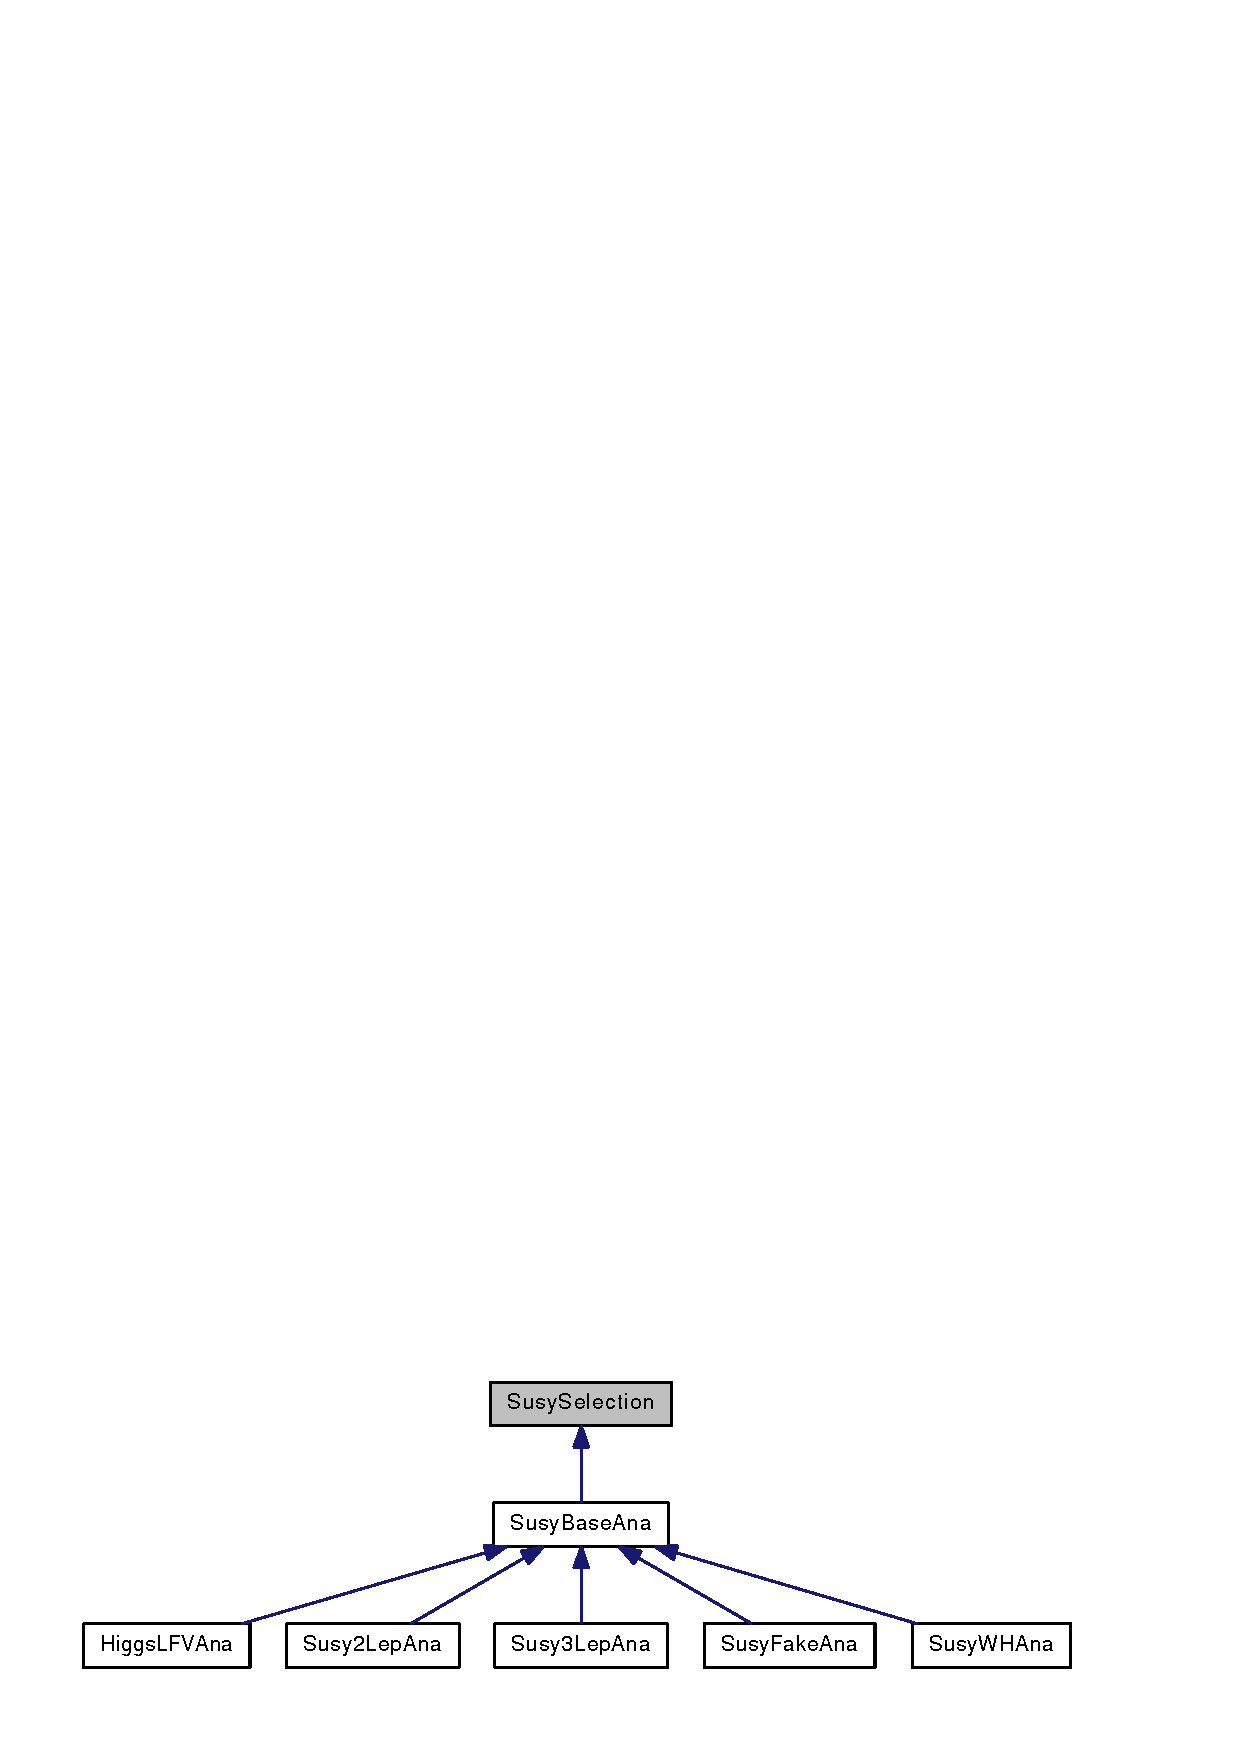
\includegraphics[width=400pt]{classSusySelection__inherit__graph}
\end{center}
\end{figure}
\subsection*{Public Member Functions}
\begin{DoxyCompactItemize}
\item 
\hypertarget{classSusySelection_a0c0bbc8c7eb7d55c7825ea03e8d2bf0d}{
{\bfseries SusySelection} (bool is2LAna=false, bool qFlipd0=true)}
\label{classSusySelection_a0c0bbc8c7eb7d55c7825ea03e8d2bf0d}

\item 
\hypertarget{classSusySelection_a25d75f7c3c1ed611f41c9aeed4c04e94}{
void {\bfseries setDebug} (int dbg)}
\label{classSusySelection_a25d75f7c3c1ed611f41c9aeed4c04e94}

\item 
\hypertarget{classSusySelection_a7552f682d0145fa5a87c5addc670e357}{
int {\bfseries dbg} ()}
\label{classSusySelection_a7552f682d0145fa5a87c5addc670e357}

\item 
\hypertarget{classSusySelection_a97533b6f715feb06b783474cfc608bd0}{
void {\bfseries resetCuts} ()}
\label{classSusySelection_a97533b6f715feb06b783474cfc608bd0}

\item 
\hypertarget{classSusySelection_ab0ceb5c31c9338c073128354ef1113ce}{
void {\bfseries reset} ()}
\label{classSusySelection_ab0ceb5c31c9338c073128354ef1113ce}

\item 
\hypertarget{classSusySelection_a212c48a8e8a0e0ac7b70b34dff4328b6}{
void {\bfseries resetCounter} ()}
\label{classSusySelection_a212c48a8e8a0e0ac7b70b34dff4328b6}

\item 
\hypertarget{classSusySelection_a71bdb5bdc5ae45eb68a896aecc83fbec}{
bool {\bfseries passEventCleaning} ()}
\label{classSusySelection_a71bdb5bdc5ae45eb68a896aecc83fbec}

\item 
\hypertarget{classSusySelection_a4fd225d1667ac6a4fa81b973c636b8b8}{
bool {\bfseries passBadFCAL} (const JetVector $\ast$jets, int run, bool isMC=false)}
\label{classSusySelection_a4fd225d1667ac6a4fa81b973c636b8b8}

\item 
\hypertarget{classSusySelection_adae424641b1d191b8a74972825a88413}{
bool {\bfseries passMll20} (const LeptonVector $\ast$leptons)}
\label{classSusySelection_adae424641b1d191b8a74972825a88413}

\item 
\hypertarget{classSusySelection_a590f5edfb2d7ec0ef3c25fcd1ce12c12}{
bool {\bfseries passTrigger} (const LeptonVector $\ast$leptons, DilTrigLogic $\ast$trigObj, const Met $\ast$met)}
\label{classSusySelection_a590f5edfb2d7ec0ef3c25fcd1ce12c12}

\item 
\hypertarget{classSusySelection_a19864d6bf1229f015d9e01593d478671}{
bool {\bfseries pass3LTrigger} (const LeptonVector $\ast$leptons, const TauVector $\ast$taus, TrilTrigLogic $\ast$trig3LObj)}
\label{classSusySelection_a19864d6bf1229f015d9e01593d478671}

\item 
\hypertarget{classSusySelection_a80ade4cf204b7599c09d706c027c7870}{
bool {\bfseries passTauVeto} (const TauVector $\ast$taus)}
\label{classSusySelection_a80ade4cf204b7599c09d706c027c7870}

\item 
\hypertarget{classSusySelection_a20f0111e9bb7d42b3d29fadad89704fc}{
bool {\bfseries passNLepCut} (const LeptonVector $\ast$leptons)}
\label{classSusySelection_a20f0111e9bb7d42b3d29fadad89704fc}

\item 
\hypertarget{classSusySelection_a9fd596d0bea0c19e7f01ec6e65000557}{
bool {\bfseries passNBase3LepCut} (const LeptonVector $\ast$leptons)}
\label{classSusySelection_a9fd596d0bea0c19e7f01ec6e65000557}

\item 
\hypertarget{classSusySelection_a548e38ba694d805031ec047a1031774b}{
bool {\bfseries passNBase4LepCut} (const LeptonVector $\ast$leptons)}
\label{classSusySelection_a548e38ba694d805031ec047a1031774b}

\item 
\hypertarget{classSusySelection_ae7013aa2c4be94858563c091ddc241dc}{
bool {\bfseries passNLep3Cut} (const LeptonVector $\ast$leptons)}
\label{classSusySelection_ae7013aa2c4be94858563c091ddc241dc}

\item 
\hypertarget{classSusySelection_a81d375efbb5d32d3f59d5f5071381d4b}{
bool {\bfseries passNLep4Cut} (const LeptonVector $\ast$leptons)}
\label{classSusySelection_a81d375efbb5d32d3f59d5f5071381d4b}

\item 
\hypertarget{classSusySelection_a67c9df2902272cc7375d6317197cfb0d}{
bool {\bfseries passIsPromptLepton} (const LeptonVector $\ast$leptons, int method, bool isMC=false)}
\label{classSusySelection_a67c9df2902272cc7375d6317197cfb0d}

\item 
\hypertarget{classSusySelection_a522e8adad0bdcc52cf5d6f8b90ef8bf3}{
bool {\bfseries passFlavor} (const LeptonVector $\ast$leptons)}
\label{classSusySelection_a522e8adad0bdcc52cf5d6f8b90ef8bf3}

\item 
\hypertarget{classSusySelection_acddc0a4aa16ce6c3a116a13996d1d27c}{
bool {\bfseries passQQ} (const LeptonVector $\ast$leptons)}
\label{classSusySelection_acddc0a4aa16ce6c3a116a13996d1d27c}

\item 
\hypertarget{classSusySelection_a5c191b0005e0461f380081b75abd8fc6}{
bool {\bfseries passFullJetVeto} (const JetVector $\ast$jets)}
\label{classSusySelection_a5c191b0005e0461f380081b75abd8fc6}

\item 
\hypertarget{classSusySelection_a7e5c74cf10b72af89ccc7d4c17f461e8}{
bool {\bfseries passZVeto} (const LeptonVector $\ast$leptons, bool useOS=true, float Zlow=MZ-\/10, float Zhigh=MZ+10)}
\label{classSusySelection_a7e5c74cf10b72af89ccc7d4c17f461e8}

\item 
\hypertarget{classSusySelection_a9c154466e051070d29510b0c78f4aa78}{
bool {\bfseries passMETRel} (const Met $\ast$met, const LeptonVector $\ast$leptons, const JetVector $\ast$jets)}
\label{classSusySelection_a9c154466e051070d29510b0c78f4aa78}

\item 
\hypertarget{classSusySelection_a5f41d29778b214ae2e8e9ae25e744163}{
bool {\bfseries passMET} (const Met $\ast$met)}
\label{classSusySelection_a5f41d29778b214ae2e8e9ae25e744163}

\item 
\hypertarget{classSusySelection_a4b1029ab2c2f6a0b0c73bb7197b424c9}{
bool {\bfseries passFJet} (const JetVector $\ast$jets)}
\label{classSusySelection_a4b1029ab2c2f6a0b0c73bb7197b424c9}

\item 
\hypertarget{classSusySelection_a008450c31f3409af1244c4ac0ed4c1ce}{
bool {\bfseries passBJet} (const JetVector $\ast$jets)}
\label{classSusySelection_a008450c31f3409af1244c4ac0ed4c1ce}

\item 
\hypertarget{classSusySelection_afb40e9bde35fff7abe9a9499e052405b}{
bool {\bfseries passLJet} (const JetVector $\ast$jets)}
\label{classSusySelection_afb40e9bde35fff7abe9a9499e052405b}

\item 
\hypertarget{classSusySelection_a935740bc99ee7d8be2e7af978f1df2bc}{
bool {\bfseries passCentralJet} (const JetVector $\ast$jets)}
\label{classSusySelection_a935740bc99ee7d8be2e7af978f1df2bc}

\item 
\hypertarget{classSusySelection_a913b23f64f3dc18851fa309e4f955a90}{
bool {\bfseries passNBJet} (const JetVector $\ast$jets)}
\label{classSusySelection_a913b23f64f3dc18851fa309e4f955a90}

\item 
\hypertarget{classSusySelection_ac38c65729b8c8314e66761b8b41b3e87}{
bool {\bfseries passLead2JetsPt} (const JetVector $\ast$jets)}
\label{classSusySelection_ac38c65729b8c8314e66761b8b41b3e87}

\item 
\hypertarget{classSusySelection_ab3e66b5ecc7e4957ea6778ba8884ff52}{
bool {\bfseries passMjj} (const JetVector $\ast$jets)}
\label{classSusySelection_ab3e66b5ecc7e4957ea6778ba8884ff52}

\item 
\hypertarget{classSusySelection_a0ee9082c587a1747bb12f9d2fe5a95d8}{
bool {\bfseries passMljj} (const LeptonVector $\ast$leptons, const JetVector $\ast$jets)}
\label{classSusySelection_a0ee9082c587a1747bb12f9d2fe5a95d8}

\item 
\hypertarget{classSusySelection_aec6048d2b882a6592e03c95a7c6144cb}{
bool {\bfseries passMT2} (const LeptonVector $\ast$leptons, const Met $\ast$met)}
\label{classSusySelection_aec6048d2b882a6592e03c95a7c6144cb}

\item 
\hypertarget{classSusySelection_a83e7386477839c9bdbb5179c4de2e247}{
bool {\bfseries passMaxMT} (const LeptonVector $\ast$leptons, const Met $\ast$met)}
\label{classSusySelection_a83e7386477839c9bdbb5179c4de2e247}

\item 
\hypertarget{classSusySelection_a62ba113cdd5089283e8fa2a0fc134b73}{
bool {\bfseries passMWWT} (const LeptonVector $\ast$leptons, const Met $\ast$met)}
\label{classSusySelection_a62ba113cdd5089283e8fa2a0fc134b73}

\item 
\hypertarget{classSusySelection_a4119c6302771d707451db0a60c3fd735}{
bool {\bfseries passMll} (const LeptonVector $\ast$leptons)}
\label{classSusySelection_a4119c6302771d707451db0a60c3fd735}

\item 
\hypertarget{classSusySelection_a0f1055afeb5e2b1579f8ac6418f8d0cf}{
bool {\bfseries passTopTagger} (const LeptonVector $\ast$leptons, const JetVector $\ast$jets, const Met $\ast$met)}
\label{classSusySelection_a0f1055afeb5e2b1579f8ac6418f8d0cf}

\item 
\hypertarget{classSusySelection_af46c8fd35547ae21d73db2c5bbcc0697}{
bool {\bfseries passLead2LepPt} (const LeptonVector $\ast$leptons)}
\label{classSusySelection_af46c8fd35547ae21d73db2c5bbcc0697}

\item 
\hypertarget{classSusySelection_a7f5e13d0fe73c8d1d4995ef9835cd52c}{
bool {\bfseries passMuoIso} (const LeptonVector $\ast$leptons, bool useRelative=true)}
\label{classSusySelection_a7f5e13d0fe73c8d1d4995ef9835cd52c}

\item 
\hypertarget{classSusySelection_a77220b086659528a43d317d64da3a98f}{
bool {\bfseries passEleD0S} (const LeptonVector $\ast$leptons)}
\label{classSusySelection_a77220b086659528a43d317d64da3a98f}

\item 
\hypertarget{classSusySelection_a40489f26ecbc15fa815ca9fb39e28b83}{
bool {\bfseries passPtll} (const LeptonVector $\ast$leptons)}
\label{classSusySelection_a40489f26ecbc15fa815ca9fb39e28b83}

\item 
\hypertarget{classSusySelection_a9b4876b736fb9b3e4b3c1433d5fa4041}{
bool {\bfseries passPtllBound} (const LeptonVector $\ast$leptons)}
\label{classSusySelection_a9b4876b736fb9b3e4b3c1433d5fa4041}

\item 
\hypertarget{classSusySelection_a11ad872e9954d0b691eeb76cbb14bf21}{
bool {\bfseries passDPhiMetll} (const LeptonVector $\ast$leptons, const Met $\ast$met)}
\label{classSusySelection_a11ad872e9954d0b691eeb76cbb14bf21}

\item 
\hypertarget{classSusySelection_a04718f3f91b54c806e1cbcf6690f11bf}{
bool {\bfseries passDPhiMetl1} (const LeptonVector $\ast$leptons, const Met $\ast$met)}
\label{classSusySelection_a04718f3f91b54c806e1cbcf6690f11bf}

\item 
\hypertarget{classSusySelection_ab58ab677b132b95ffd499f5aaeef0ec5}{
bool {\bfseries passdPhi} (TLorentzVector v0, TLorentzVector v1, float cut)}
\label{classSusySelection_ab58ab677b132b95ffd499f5aaeef0ec5}

\item 
\hypertarget{classSusySelection_a600f722df5dc953eff6fe69532196e94}{
bool {\bfseries passdPhill} (const LeptonVector $\ast$leptons)}
\label{classSusySelection_a600f722df5dc953eff6fe69532196e94}

\item 
\hypertarget{classSusySelection_a10d79039a2afaa20cf9927a45493825c}{
bool {\bfseries passdEtall} (const LeptonVector $\ast$leptons)}
\label{classSusySelection_a10d79039a2afaa20cf9927a45493825c}

\item 
\hypertarget{classSusySelection_ac08f98b3eff272a41c880a1706ae81ad}{
bool {\bfseries passdRll} (const LeptonVector $\ast$leptons)}
\label{classSusySelection_ac08f98b3eff272a41c880a1706ae81ad}

\item 
\hypertarget{classSusySelection_a045502e543160aee5e53201bff399386}{
bool {\bfseries passDPhillJ0} (const LeptonVector $\ast$leptons, const JetVector $\ast$jets)}
\label{classSusySelection_a045502e543160aee5e53201bff399386}

\item 
\hypertarget{classSusySelection_a3ab5d1b5cc09cf2acb913982f29d4191}{
bool {\bfseries passDPhillMET} (const LeptonVector $\ast$leptons, const Met $\ast$met)}
\label{classSusySelection_a3ab5d1b5cc09cf2acb913982f29d4191}

\item 
\hypertarget{classSusySelection_a01e725d50fc174908ffe297394c09458}{
bool {\bfseries passMetMeff} (const LeptonVector $\ast$leptons, const JetVector $\ast$jets, const Met $\ast$met, bool useLepton=false)}
\label{classSusySelection_a01e725d50fc174908ffe297394c09458}

\item 
\hypertarget{classSusySelection_a9376f2f9a4764e3bf8b4c28aae415aed}{
bool {\bfseries passMeff} (const JetVector $\ast$jets, const Met $\ast$met)}
\label{classSusySelection_a9376f2f9a4764e3bf8b4c28aae415aed}

\item 
\hypertarget{classSusySelection_a79d7bf361223e86d0e702916c6a5871f}{
bool {\bfseries passHT} (const LeptonVector $\ast$leptons, const JetVector $\ast$jets, const Met $\ast$met)}
\label{classSusySelection_a79d7bf361223e86d0e702916c6a5871f}

\item 
\hypertarget{classSusySelection_a40a645ea96cea584198f5f3cedfbf576}{
bool {\bfseries passSFOSLooseLepton} (SusyNtObject $\ast$susyNt, const LeptonVector leptons, float minMll=MZ-\/20, float maxMll=MZ+20)}
\label{classSusySelection_a40a645ea96cea584198f5f3cedfbf576}

\item 
\hypertarget{classSusySelection_ac991ad8ea8a6936dcd2a9637a477f76b}{
bool {\bfseries isGenuineSS} (const LeptonVector $\ast$leptons, bool isMC)}
\label{classSusySelection_ac991ad8ea8a6936dcd2a9637a477f76b}

\item 
\hypertarget{classSusySelection_a17707c06d4931380a0dd8dbe75547711}{
bool {\bfseries hasQFlip} (const LeptonVector $\ast$leptons)}
\label{classSusySelection_a17707c06d4931380a0dd8dbe75547711}

\item 
\hypertarget{classSusySelection_aaeca9dce95b5f728b5d1c58474616082}{
float {\bfseries getQFlipProb} (LeptonVector $\ast$leptons, Met $\ast$met, uint iSys=DGSys\_\-NOM)}
\label{classSusySelection_aaeca9dce95b5f728b5d1c58474616082}

\item 
\hypertarget{classSusySelection_a6cba3254d008ffe1be4cf6c85a02d779}{
bool {\bfseries passSFOSCut} (const LeptonVector $\ast$leptons)}
\label{classSusySelection_a6cba3254d008ffe1be4cf6c85a02d779}

\item 
\hypertarget{classSusySelection_a46b6f21683b076e328a97eddc168cfc4}{
bool {\bfseries passZCut} (const LeptonVector $\ast$leptons)}
\label{classSusySelection_a46b6f21683b076e328a97eddc168cfc4}

\item 
\hypertarget{classSusySelection_a5fab6541be2450d036e230ed9741c78d}{
bool {\bfseries passZllZll} (const LeptonVector $\ast$leptons)}
\label{classSusySelection_a5fab6541be2450d036e230ed9741c78d}

\item 
\hypertarget{classSusySelection_a5fd34dcaf46ceb590c078bdd11c53b82}{
bool {\bfseries passMtCut} (const LeptonVector $\ast$leptons, const Met $\ast$met)}
\label{classSusySelection_a5fd34dcaf46ceb590c078bdd11c53b82}

\item 
\hypertarget{classSusySelection_ac25cafa9caa25b0ee586184f339997e6}{
float {\bfseries JZBJet} (const JetVector $\ast$jets, const LeptonVector $\ast$leptons)}
\label{classSusySelection_ac25cafa9caa25b0ee586184f339997e6}

\item 
\hypertarget{classSusySelection_aaeb5211e87042d218f2ce6a12da8f6aa}{
float {\bfseries JZBEtmiss} (const Met $\ast$met, const LeptonVector $\ast$leptons)}
\label{classSusySelection_aaeb5211e87042d218f2ce6a12da8f6aa}

\item 
\hypertarget{classSusySelection_a8af22548147dca3cf8f52ee63c9490de}{
bool {\bfseries emulateWW} (LeptonVector $\ast$leptons, Met $\ast$met)}
\label{classSusySelection_a8af22548147dca3cf8f52ee63c9490de}

\item 
\hypertarget{classSusySelection_a8ed69832598b39aa8e19f7ac36cbba43}{
uint {\bfseries get3LType} (const LeptonVector \&leptons)}
\label{classSusySelection_a8ed69832598b39aa8e19f7ac36cbba43}

\item 
\hypertarget{classSusySelection_ae758ee64fd51ff18ef4f22a82bbc6ec3}{
uint {\bfseries get4LType} (const LeptonVector \&leptons)}
\label{classSusySelection_ae758ee64fd51ff18ef4f22a82bbc6ec3}

\item 
\hypertarget{classSusySelection_aa9f63f4c8b3ef285fa0afcc988d3d141}{
void {\bfseries sumArray} ()}
\label{classSusySelection_aa9f63f4c8b3ef285fa0afcc988d3d141}

\item 
\hypertarget{classSusySelection_a7cb47f3c518e3ec7e10a7eff588ed943}{
LeptonVector {\bfseries findSFOSinZ} (LeptonVector $\ast$preLeptons, const LeptonVector $\ast$leptons, bool \&hasSFOSinZ, float minMll=MZ-\/20, float maxMll=MZ+20)}
\label{classSusySelection_a7cb47f3c518e3ec7e10a7eff588ed943}

\item 
\hypertarget{classSusySelection_a983d450d050c161439b0f1700d3a36cb}{
void {\bfseries getPreLeptons} (Susy::SusyNtObject $\ast$susyNt)}
\label{classSusySelection_a983d450d050c161439b0f1700d3a36cb}

\item 
\hypertarget{classSusySelection_a3591c1d69a2e120dd1c09e7187d69bc1}{
LeptonVector {\bfseries getLooseLeptons} (LeptonVector $\ast$preLeptons, const LeptonVector $\ast$leptons)}
\label{classSusySelection_a3591c1d69a2e120dd1c09e7187d69bc1}

\item 
\hypertarget{classSusySelection_a99b865915fecaf39af45b9aae76bc952}{
bool {\bfseries passBasicLeptonSelection} (const Lepton $\ast$l)}
\label{classSusySelection_a99b865915fecaf39af45b9aae76bc952}

\item 
\hypertarget{classSusySelection_acc7a9ae01cf1940c0c810f75e6a3b4a8}{
bool {\bfseries isPT} (const Lepton $\ast$lep)}
\label{classSusySelection_acc7a9ae01cf1940c0c810f75e6a3b4a8}

\item 
\hypertarget{classSusySelection_a81688a94ef2a63e95ac61fd2be607a74}{
bool {\bfseries isConv} (const Lepton $\ast$lep)}
\label{classSusySelection_a81688a94ef2a63e95ac61fd2be607a74}

\item 
\hypertarget{classSusySelection_ad097463414892067d668de453d8d5f59}{
bool {\bfseries isLF} (const Lepton $\ast$lep)}
\label{classSusySelection_ad097463414892067d668de453d8d5f59}

\item 
\hypertarget{classSusySelection_a2635c4b8f640e1d690b32e9e8a0386ba}{
bool {\bfseries isHF} (const Lepton $\ast$lep)}
\label{classSusySelection_a2635c4b8f640e1d690b32e9e8a0386ba}

\item 
\hypertarget{classSusySelection_a00e41bc9d2e4aa9aa1980e310c174556}{
bool {\bfseries isQFlip} (const Lepton $\ast$lep)}
\label{classSusySelection_a00e41bc9d2e4aa9aa1980e310c174556}

\item 
\hypertarget{classSusySelection_ab1d080bca7f083a892e5630176a0cc3e}{
LEP\_\-TYPE {\bfseries getType} (const Lepton $\ast$lep)}
\label{classSusySelection_ab1d080bca7f083a892e5630176a0cc3e}

\item 
\hypertarget{classSusySelection_a707cce86d86baa8b345a4b6ca3ff9ab1}{
{\bfseries ClassDef} (\hyperlink{classSusySelection}{SusySelection}, 1)}
\label{classSusySelection_a707cce86d86baa8b345a4b6ca3ff9ab1}

\end{DoxyCompactItemize}
\subsection*{Protected Attributes}
\begin{DoxyCompactItemize}
\item 
\hypertarget{classSusySelection_ab56927fd4ab7c381dd2d1768f160588b}{
TRandom3 $\ast$ {\bfseries \_\-random}}
\label{classSusySelection_ab56927fd4ab7c381dd2d1768f160588b}

\item 
\hypertarget{classSusySelection_a81c6485b02e2fdc0edbf031c0a4defc8}{
Susy::SusyNtObject $\ast$ {\bfseries nt}}
\label{classSusySelection_a81c6485b02e2fdc0edbf031c0a4defc8}

\item 
\hypertarget{classSusySelection_a9812ace735a65f9832c9cdb0ef54a664}{
int {\bfseries m\_\-dbg}}
\label{classSusySelection_a9812ace735a65f9832c9cdb0ef54a664}

\item 
\hypertarget{classSusySelection_a77a194d88d7bd9e528308a57d3a53e1b}{
chargeFlip $\ast$ {\bfseries m\_\-chargeFlip}}
\label{classSusySelection_a77a194d88d7bd9e528308a57d3a53e1b}

\item 
\hypertarget{classSusySelection_a41ba58dd502d67a720a46cff5f2333aa}{
ElectronVector $\ast$ {\bfseries v\_\-preEle}}
\label{classSusySelection_a41ba58dd502d67a720a46cff5f2333aa}

\item 
\hypertarget{classSusySelection_a42ccbf4f103b9acdcd88ab784cd84fd4}{
MuonVector $\ast$ {\bfseries v\_\-preMu}}
\label{classSusySelection_a42ccbf4f103b9acdcd88ab784cd84fd4}

\item 
\hypertarget{classSusySelection_ae3fc9f54dfe38174b3696c70e4268ff7}{
LeptonVector {\bfseries v\_\-preLep}}
\label{classSusySelection_ae3fc9f54dfe38174b3696c70e4268ff7}

\item 
\hypertarget{classSusySelection_a30312808cd6a3135d7aa93ef18b9ecce}{
JetVector $\ast$ {\bfseries v\_\-preJet}}
\label{classSusySelection_a30312808cd6a3135d7aa93ef18b9ecce}

\item 
\hypertarget{classSusySelection_a3a0d0a775686274cfed8b417d723c0ee}{
ElectronVector $\ast$ {\bfseries v\_\-baseEle}}
\label{classSusySelection_a3a0d0a775686274cfed8b417d723c0ee}

\item 
\hypertarget{classSusySelection_aeac8fbc4019705794e397490ae1c7878}{
ElectronVector $\ast$ {\bfseries v\_\-sigEle}}
\label{classSusySelection_aeac8fbc4019705794e397490ae1c7878}

\item 
\hypertarget{classSusySelection_a3de45df594f44594fef8b190deea8808}{
MuonVector $\ast$ {\bfseries v\_\-baseMu}}
\label{classSusySelection_a3de45df594f44594fef8b190deea8808}

\item 
\hypertarget{classSusySelection_a508e3ba0e574e472fa062dd3d4c5b77e}{
MuonVector $\ast$ {\bfseries v\_\-sigMu}}
\label{classSusySelection_a508e3ba0e574e472fa062dd3d4c5b77e}

\item 
\hypertarget{classSusySelection_ac733a0ec3057fd9a76e25c9b1315e836}{
LeptonVector $\ast$ {\bfseries v\_\-baseLep}}
\label{classSusySelection_ac733a0ec3057fd9a76e25c9b1315e836}

\item 
\hypertarget{classSusySelection_a8c1c1aa0a1daf9e8989367331d760bcf}{
LeptonVector $\ast$ {\bfseries v\_\-sigLep}}
\label{classSusySelection_a8c1c1aa0a1daf9e8989367331d760bcf}

\item 
\hypertarget{classSusySelection_a9494f37846904879fd2ad1c38357f4d4}{
JetVector $\ast$ {\bfseries v\_\-baseJet}}
\label{classSusySelection_a9494f37846904879fd2ad1c38357f4d4}

\item 
\hypertarget{classSusySelection_ac235fcc9c56765f8e4b27844686aa2c9}{
JetVector $\ast$ {\bfseries v\_\-sigJet}}
\label{classSusySelection_ac235fcc9c56765f8e4b27844686aa2c9}

\item 
\hypertarget{classSusySelection_ad26b55cb3dc75b04f225441b2525e820}{
TauVector $\ast$ {\bfseries v\_\-baseTau}}
\label{classSusySelection_ad26b55cb3dc75b04f225441b2525e820}

\item 
\hypertarget{classSusySelection_a4d45f9e9491e616b2048d5919deccfb5}{
TauVector $\ast$ {\bfseries v\_\-sigTau}}
\label{classSusySelection_a4d45f9e9491e616b2048d5919deccfb5}

\item 
\hypertarget{classSusySelection_ac0664a5db5f37d5d1061fc0e73f9253d}{
const Susy::Met $\ast$ {\bfseries m\_\-met}}
\label{classSusySelection_ac0664a5db5f37d5d1061fc0e73f9253d}

\item 
\hypertarget{classSusySelection_a9fd107ec640a01a064bf4187d02f5b68}{
ElectronVector {\bfseries v\_\-save\_\-sigEle}}
\label{classSusySelection_a9fd107ec640a01a064bf4187d02f5b68}

\item 
\hypertarget{classSusySelection_ac7b47317531692bd8a154299341e39e6}{
MuonVector {\bfseries v\_\-save\_\-sigMu}}
\label{classSusySelection_ac7b47317531692bd8a154299341e39e6}

\item 
\hypertarget{classSusySelection_a4369555ec81a226f058d71404e493494}{
LeptonVector {\bfseries v\_\-save\_\-sigLep}}
\label{classSusySelection_a4369555ec81a226f058d71404e493494}

\item 
\hypertarget{classSusySelection_a2bfec0ba8a3730ddfaab249bb187e0f1}{
Susy::Met {\bfseries new\_\-met}}
\label{classSusySelection_a2bfec0ba8a3730ddfaab249bb187e0f1}

\item 
\hypertarget{classSusySelection_ae09047168c0327279d16ed83a3ac97a9}{
float {\bfseries \_\-inc}}
\label{classSusySelection_ae09047168c0327279d16ed83a3ac97a9}

\item 
\hypertarget{classSusySelection_a171a00af58fbc24353399700c387769e}{
uint {\bfseries SR}}
\label{classSusySelection_a171a00af58fbc24353399700c387769e}

\item 
\hypertarget{classSusySelection_a7e9bcb9956607c5c20938b42e2d83cad}{
uint {\bfseries SYST}}
\label{classSusySelection_a7e9bcb9956607c5c20938b42e2d83cad}

\item 
\hypertarget{classSusySelection_a739b17a65aec375121b6b583e6924a01}{
bool {\bfseries m\_\-cutNBaseLep}}
\label{classSusySelection_a739b17a65aec375121b6b583e6924a01}

\item 
\hypertarget{classSusySelection_a67fdc0b4474104c2bb07f0f07a3294d5}{
uint {\bfseries m\_\-nLepMin}}
\label{classSusySelection_a67fdc0b4474104c2bb07f0f07a3294d5}

\item 
\hypertarget{classSusySelection_ae38d5bf935cf0661fcd3101fb6a66e81}{
uint {\bfseries m\_\-nLepMax}}
\label{classSusySelection_ae38d5bf935cf0661fcd3101fb6a66e81}

\item 
\hypertarget{classSusySelection_a2a6a5d3f7a2a28bb8ae5b522f4029094}{
uint {\bfseries m\_\-nLep3Min}}
\label{classSusySelection_a2a6a5d3f7a2a28bb8ae5b522f4029094}

\item 
\hypertarget{classSusySelection_a6cb685cf47d8f529eb7db22c387c9415}{
uint {\bfseries m\_\-nLep3Max}}
\label{classSusySelection_a6cb685cf47d8f529eb7db22c387c9415}

\item 
\hypertarget{classSusySelection_a46d159d491220645e62df9a6f007c7a7}{
uint {\bfseries m\_\-nLep4Min}}
\label{classSusySelection_a46d159d491220645e62df9a6f007c7a7}

\item 
\hypertarget{classSusySelection_a5c50e777fcfbeb21dda646d24e6760ac}{
uint {\bfseries m\_\-nLep4Max}}
\label{classSusySelection_a5c50e777fcfbeb21dda646d24e6760ac}

\item 
\hypertarget{classSusySelection_ac334d390bfec42d884324f88f1624423}{
bool {\bfseries m\_\-selOS}}
\label{classSusySelection_ac334d390bfec42d884324f88f1624423}

\item 
\hypertarget{classSusySelection_a6dbe8321a38595b947f430d0d343df8e}{
bool {\bfseries m\_\-selSS}}
\label{classSusySelection_a6dbe8321a38595b947f430d0d343df8e}

\item 
\hypertarget{classSusySelection_a04d29887835ca561dc93cfbd89d28911}{
bool {\bfseries m\_\-selSF}}
\label{classSusySelection_a04d29887835ca561dc93cfbd89d28911}

\item 
\hypertarget{classSusySelection_ad3a9e05e013b7bd4d8f16c6597747473}{
bool {\bfseries m\_\-selOF}}
\label{classSusySelection_ad3a9e05e013b7bd4d8f16c6597747473}

\item 
\hypertarget{classSusySelection_a53f8e12410b67760204ba0e9527e4f76}{
bool {\bfseries m\_\-vetoSF}}
\label{classSusySelection_a53f8e12410b67760204ba0e9527e4f76}

\item 
\hypertarget{classSusySelection_a672a9a50fd1eb9810d702e5312278660}{
bool {\bfseries m\_\-selSFOS}}
\label{classSusySelection_a672a9a50fd1eb9810d702e5312278660}

\item 
\hypertarget{classSusySelection_a36e235a34d04762c01923902ea8e74ce}{
bool {\bfseries m\_\-vetoSFOS}}
\label{classSusySelection_a36e235a34d04762c01923902ea8e74ce}

\item 
\hypertarget{classSusySelection_a760d5ff9fa317759f86176a30f1bb194}{
bool {\bfseries m\_\-selZ}}
\label{classSusySelection_a760d5ff9fa317759f86176a30f1bb194}

\item 
\hypertarget{classSusySelection_a4276599c1e85d515e7c18569ef4fc5b7}{
bool {\bfseries m\_\-vetoZ}}
\label{classSusySelection_a4276599c1e85d515e7c18569ef4fc5b7}

\item 
\hypertarget{classSusySelection_a0c35d9e6d84346a916eb297a2ae60050}{
bool {\bfseries m\_\-vetoExtZ}}
\label{classSusySelection_a0c35d9e6d84346a916eb297a2ae60050}

\item 
\hypertarget{classSusySelection_a562cb3eb5dd575598dbfac2f05d49a2a}{
bool {\bfseries m\_\-selZllZll}}
\label{classSusySelection_a562cb3eb5dd575598dbfac2f05d49a2a}

\item 
\hypertarget{classSusySelection_ad9a90abcf96989688809824f5ae7f844}{
bool {\bfseries m\_\-selB}}
\label{classSusySelection_ad9a90abcf96989688809824f5ae7f844}

\item 
\hypertarget{classSusySelection_ab61e33a60133f1a56610707cd5d7bd72}{
bool {\bfseries m\_\-vetoB}}
\label{classSusySelection_ab61e33a60133f1a56610707cd5d7bd72}

\item 
\hypertarget{classSusySelection_a503980808acc95a09e01422eb5324643}{
bool {\bfseries m\_\-vetoF}}
\label{classSusySelection_a503980808acc95a09e01422eb5324643}

\item 
\hypertarget{classSusySelection_a25a412a1adb60bd342e1cad32eb6c0bd}{
bool {\bfseries m\_\-vetoJ}}
\label{classSusySelection_a25a412a1adb60bd342e1cad32eb6c0bd}

\item 
\hypertarget{classSusySelection_aee03f2d42b6a5b1f12a65741b4728178}{
int {\bfseries m\_\-minC20}}
\label{classSusySelection_aee03f2d42b6a5b1f12a65741b4728178}

\item 
\hypertarget{classSusySelection_a9d4cfefee407e8b36a32a29a268d4e71}{
int {\bfseries m\_\-maxC20}}
\label{classSusySelection_a9d4cfefee407e8b36a32a29a268d4e71}

\item 
\hypertarget{classSusySelection_a97ab306348f92d903f5b3822f414b993}{
int {\bfseries m\_\-minCJet}}
\label{classSusySelection_a97ab306348f92d903f5b3822f414b993}

\item 
\hypertarget{classSusySelection_a1e70d69f5f7595d0348aad727ca47b72}{
int {\bfseries m\_\-minB20}}
\label{classSusySelection_a1e70d69f5f7595d0348aad727ca47b72}

\item 
\hypertarget{classSusySelection_a7e62e5fc1505c695157d4a555e10dd8c}{
int {\bfseries m\_\-maxB20}}
\label{classSusySelection_a7e62e5fc1505c695157d4a555e10dd8c}

\item 
\hypertarget{classSusySelection_acea3f6232c68351a2006d564cf1fa9ec}{
float {\bfseries m\_\-metMin}}
\label{classSusySelection_acea3f6232c68351a2006d564cf1fa9ec}

\item 
\hypertarget{classSusySelection_a1ceeb9f8935691fe22f11f5e68719720}{
float {\bfseries m\_\-metMax}}
\label{classSusySelection_a1ceeb9f8935691fe22f11f5e68719720}

\item 
\hypertarget{classSusySelection_a511ac42fecd574b460948dd118beae2d}{
float {\bfseries m\_\-metRelMin}}
\label{classSusySelection_a511ac42fecd574b460948dd118beae2d}

\item 
\hypertarget{classSusySelection_a459d28ed6405db40fcf84b0f6800678f}{
float {\bfseries m\_\-metRelMax}}
\label{classSusySelection_a459d28ed6405db40fcf84b0f6800678f}

\item 
\hypertarget{classSusySelection_acb0c55733180b382364d74549e5b5d48}{
bool {\bfseries m\_\-topTag}}
\label{classSusySelection_acb0c55733180b382364d74549e5b5d48}

\item 
\hypertarget{classSusySelection_a5d9bf225b1bc194914423a87ad7c9c2b}{
float {\bfseries m\_\-mt2Min}}
\label{classSusySelection_a5d9bf225b1bc194914423a87ad7c9c2b}

\item 
\hypertarget{classSusySelection_afe8d384ebd48750b3a7a74a09a308ba5}{
float {\bfseries m\_\-mt2Max}}
\label{classSusySelection_afe8d384ebd48750b3a7a74a09a308ba5}

\item 
\hypertarget{classSusySelection_a200697c815878de8b5a9f30670c556f2}{
float {\bfseries m\_\-mtMin}}
\label{classSusySelection_a200697c815878de8b5a9f30670c556f2}

\item 
\hypertarget{classSusySelection_a4d9b4f279da14bd686a6b3b16cd1bf1f}{
float {\bfseries m\_\-mtMax}}
\label{classSusySelection_a4d9b4f279da14bd686a6b3b16cd1bf1f}

\item 
\hypertarget{classSusySelection_afa2e8a2ac6bb33d9cc49e9b2dfa63258}{
float {\bfseries m\_\-mtMaxLow}}
\label{classSusySelection_afa2e8a2ac6bb33d9cc49e9b2dfa63258}

\item 
\hypertarget{classSusySelection_a48d55f0f4812843cb68cba176ff30b0a}{
float {\bfseries m\_\-mtMaxHigh}}
\label{classSusySelection_a48d55f0f4812843cb68cba176ff30b0a}

\item 
\hypertarget{classSusySelection_ab146c7b4cc62b960eb04cf5d3b7ef30a}{
float {\bfseries m\_\-lepLeadPtMin}}
\label{classSusySelection_ab146c7b4cc62b960eb04cf5d3b7ef30a}

\item 
\hypertarget{classSusySelection_a97ef926a78dcfcf4d96842f77db6e199}{
float {\bfseries m\_\-pTl0Min}}
\label{classSusySelection_a97ef926a78dcfcf4d96842f77db6e199}

\item 
\hypertarget{classSusySelection_ac410a5fd7f5c0fd525da65df23b8ec6d}{
float {\bfseries m\_\-pTl1Min}}
\label{classSusySelection_ac410a5fd7f5c0fd525da65df23b8ec6d}

\item 
\hypertarget{classSusySelection_aea5a78a1020c0c428ebf6635bc3d50c0}{
float {\bfseries m\_\-pTl1Max}}
\label{classSusySelection_aea5a78a1020c0c428ebf6635bc3d50c0}

\item 
\hypertarget{classSusySelection_a4ee955ebc420cebd1a9e6affa5561bd1}{
float {\bfseries m\_\-IsoMin}}
\label{classSusySelection_a4ee955ebc420cebd1a9e6affa5561bd1}

\item 
\hypertarget{classSusySelection_a6a2d484da040abc290671b3f5e0cbcab}{
float {\bfseries m\_\-d0SMin}}
\label{classSusySelection_a6a2d484da040abc290671b3f5e0cbcab}

\item 
\hypertarget{classSusySelection_ad623ad36a0b284080aeeda36ecc2df3a}{
float {\bfseries m\_\-pTllMin}}
\label{classSusySelection_ad623ad36a0b284080aeeda36ecc2df3a}

\item 
\hypertarget{classSusySelection_ad42e679e1eb1569fb157e5331fa66b8c}{
float {\bfseries m\_\-pTllMax}}
\label{classSusySelection_ad42e679e1eb1569fb157e5331fa66b8c}

\item 
\hypertarget{classSusySelection_aee1c9917ce0e439b6e1dfbecc0cfd672}{
bool {\bfseries m\_\-pTllBound}}
\label{classSusySelection_aee1c9917ce0e439b6e1dfbecc0cfd672}

\item 
\hypertarget{classSusySelection_a51a0f9e15654ceff6d86d8aa14035ae1}{
float {\bfseries m\_\-lowMll}}
\label{classSusySelection_a51a0f9e15654ceff6d86d8aa14035ae1}

\item 
\hypertarget{classSusySelection_abd1f58f5eeb3ef751402e344cb46b19c}{
float {\bfseries m\_\-highMll}}
\label{classSusySelection_abd1f58f5eeb3ef751402e344cb46b19c}

\item 
\hypertarget{classSusySelection_a64910aa5929b7def4e00b07c4fc7e123}{
bool {\bfseries m\_\-mllIn}}
\label{classSusySelection_a64910aa5929b7def4e00b07c4fc7e123}

\item 
\hypertarget{classSusySelection_a1a5722c9890a2cc6c873dba7891cc7ac}{
float {\bfseries m\_\-dPhillMax}}
\label{classSusySelection_a1a5722c9890a2cc6c873dba7891cc7ac}

\item 
\hypertarget{classSusySelection_aa270f1642053b6e21c41849c5aad5471}{
float {\bfseries m\_\-dPhillMin}}
\label{classSusySelection_aa270f1642053b6e21c41849c5aad5471}

\item 
\hypertarget{classSusySelection_a35bcba08419f53d4576601d00252d5de}{
float {\bfseries m\_\-dEtallMax}}
\label{classSusySelection_a35bcba08419f53d4576601d00252d5de}

\item 
\hypertarget{classSusySelection_aca8e463e541ccc632736a27f22513052}{
float {\bfseries m\_\-dRllMin}}
\label{classSusySelection_aca8e463e541ccc632736a27f22513052}

\item 
\hypertarget{classSusySelection_a315bf88ed4b808a2ec749396d2e2d7aa}{
float {\bfseries m\_\-dRllMax}}
\label{classSusySelection_a315bf88ed4b808a2ec749396d2e2d7aa}

\item 
\hypertarget{classSusySelection_a6f39c2ac2682de4242e7a6c00e697c7a}{
float {\bfseries m\_\-lowMjj}}
\label{classSusySelection_a6f39c2ac2682de4242e7a6c00e697c7a}

\item 
\hypertarget{classSusySelection_ac5aa328e742a0ea4927fc02eab5ef319}{
float {\bfseries m\_\-highMjj}}
\label{classSusySelection_ac5aa328e742a0ea4927fc02eab5ef319}

\item 
\hypertarget{classSusySelection_adeb1359723319f283677f31819467895}{
float {\bfseries m\_\-highMljj}}
\label{classSusySelection_adeb1359723319f283677f31819467895}

\item 
\hypertarget{classSusySelection_a5ecc82ce7c94bdd10e9905216559a22e}{
float {\bfseries m\_\-lowMljj}}
\label{classSusySelection_a5ecc82ce7c94bdd10e9905216559a22e}

\item 
\hypertarget{classSusySelection_a14025ba6ac6e12b0f6f9e46af4e5b6c1}{
float {\bfseries m\_\-lowMTWW}}
\label{classSusySelection_a14025ba6ac6e12b0f6f9e46af4e5b6c1}

\item 
\hypertarget{classSusySelection_a2fa002fae9a8300c0a15c720f22f2d1b}{
float {\bfseries m\_\-highMTWW}}
\label{classSusySelection_a2fa002fae9a8300c0a15c720f22f2d1b}

\item 
\hypertarget{classSusySelection_a07236e60db23021d6eb548f468171671}{
float {\bfseries m\_\-pTj0Min}}
\label{classSusySelection_a07236e60db23021d6eb548f468171671}

\item 
\hypertarget{classSusySelection_aa4872cb43a0c3beeeba6513d19d0f0f1}{
float {\bfseries m\_\-pTj1Min}}
\label{classSusySelection_aa4872cb43a0c3beeeba6513d19d0f0f1}

\item 
\hypertarget{classSusySelection_a068e165beded3c8932b63f56dcf4546e}{
float {\bfseries m\_\-dPhiMetll}}
\label{classSusySelection_a068e165beded3c8932b63f56dcf4546e}

\item 
\hypertarget{classSusySelection_ac3b03a48904bc28687619f1a9290a425}{
float {\bfseries m\_\-dPhiMetl1}}
\label{classSusySelection_ac3b03a48904bc28687619f1a9290a425}

\item 
\hypertarget{classSusySelection_ad081e47be586f2f37a07d113fa2e4591}{
float {\bfseries m\_\-dPhillJ0Min}}
\label{classSusySelection_ad081e47be586f2f37a07d113fa2e4591}

\item 
\hypertarget{classSusySelection_a0200593090c1546ac529dc1296f6bd18}{
float {\bfseries m\_\-dPhillJ0Max}}
\label{classSusySelection_a0200593090c1546ac529dc1296f6bd18}

\item 
\hypertarget{classSusySelection_abc1f28a66ec5352f44378f7294e4e420}{
float {\bfseries m\_\-dPhillMetMin}}
\label{classSusySelection_abc1f28a66ec5352f44378f7294e4e420}

\item 
\hypertarget{classSusySelection_a9133e6de0fbecfd359401a88fd1b1d96}{
float {\bfseries m\_\-dPhillMetMax}}
\label{classSusySelection_a9133e6de0fbecfd359401a88fd1b1d96}

\item 
\hypertarget{classSusySelection_ad2a13a6c5c7a99920c2935ed178c5f52}{
float {\bfseries m\_\-MetMeffMin}}
\label{classSusySelection_ad2a13a6c5c7a99920c2935ed178c5f52}

\item 
\hypertarget{classSusySelection_a29cd94d0cf5e5400f581558648058ad2}{
float {\bfseries m\_\-MetMeffMax}}
\label{classSusySelection_a29cd94d0cf5e5400f581558648058ad2}

\item 
\hypertarget{classSusySelection_ab458b48ed32b3d565eb2c33f33b83882}{
float {\bfseries m\_\-MeffMin}}
\label{classSusySelection_ab458b48ed32b3d565eb2c33f33b83882}

\item 
\hypertarget{classSusySelection_abf5a041bc7b4e70af78c3a789246b7b4}{
float {\bfseries m\_\-MeffMax}}
\label{classSusySelection_abf5a041bc7b4e70af78c3a789246b7b4}

\item 
\hypertarget{classSusySelection_a73d80c8983c5f35aa27cb5846ffc8f63}{
float {\bfseries m\_\-HTMin}}
\label{classSusySelection_a73d80c8983c5f35aa27cb5846ffc8f63}

\item 
\hypertarget{classSusySelection_aee234706df9a049615d3de2df3821d73}{
float {\bfseries m\_\-HTMax}}
\label{classSusySelection_aee234706df9a049615d3de2df3821d73}

\item 
\hypertarget{classSusySelection_a1a9d51dcc7b5b0c27cdf160bd5e7261e}{
bool {\bfseries m\_\-vetoLooseSFOSinZ}}
\label{classSusySelection_a1a9d51dcc7b5b0c27cdf160bd5e7261e}

\item 
\hypertarget{classSusySelection_adfa27cdc05b23b91bb6f9e9438d4a4ff}{
uint {\bfseries m\_\-ET}}
\label{classSusySelection_adfa27cdc05b23b91bb6f9e9438d4a4ff}

\item 
\hypertarget{classSusySelection_ad7657e443f3d9ddfc3667d60b404c59a}{
float {\bfseries n\_\-readin}}
\label{classSusySelection_ad7657e443f3d9ddfc3667d60b404c59a}

\item 
\hypertarget{classSusySelection_a5d06909810ba080a59c61edb581e984c}{
float {\bfseries n\_\-pass\_\-SUSYGrid}}
\label{classSusySelection_a5d06909810ba080a59c61edb581e984c}

\item 
\hypertarget{classSusySelection_a6bbc219b36b0411467e84059bef86ce1}{
float {\bfseries n\_\-pass\_\-GRL}}
\label{classSusySelection_a6bbc219b36b0411467e84059bef86ce1}

\item 
\hypertarget{classSusySelection_acb7638d6640fb135cf883c9756dca877}{
float {\bfseries n\_\-pass\_\-LarErr}}
\label{classSusySelection_acb7638d6640fb135cf883c9756dca877}

\item 
\hypertarget{classSusySelection_acad0e4961d964dc7e84ca162bb6894cf}{
float {\bfseries n\_\-pass\_\-TileErr}}
\label{classSusySelection_acad0e4961d964dc7e84ca162bb6894cf}

\item 
\hypertarget{classSusySelection_aa0e1584db681ea176357aa429c94a81f}{
float {\bfseries n\_\-pass\_\-TTCVeto}}
\label{classSusySelection_aa0e1584db681ea176357aa429c94a81f}

\item 
\hypertarget{classSusySelection_a60a5f5e1fdedec9bb8c37543eca14d85}{
float {\bfseries n\_\-pass\_\-GoodVtx}}
\label{classSusySelection_a60a5f5e1fdedec9bb8c37543eca14d85}

\item 
\hypertarget{classSusySelection_a71e9f09ad9b9e89c044e2ad3e1d055d0}{
float {\bfseries n\_\-pass\_\-TileTrip}}
\label{classSusySelection_a71e9f09ad9b9e89c044e2ad3e1d055d0}

\item 
\hypertarget{classSusySelection_a8ab309a610fd71f04179ccb8a02b9df2}{
float {\bfseries n\_\-pass\_\-HotSpot}}
\label{classSusySelection_a8ab309a610fd71f04179ccb8a02b9df2}

\item 
\hypertarget{classSusySelection_afc9ffc6285d8b8577aa0153ccf9beacd}{
float {\bfseries n\_\-pass\_\-BadJet}}
\label{classSusySelection_afc9ffc6285d8b8577aa0153ccf9beacd}

\item 
\hypertarget{classSusySelection_ab3e1868bed7083d6b5aab66a94614353}{
float {\bfseries n\_\-pass\_\-BadMuon}}
\label{classSusySelection_ab3e1868bed7083d6b5aab66a94614353}

\item 
\hypertarget{classSusySelection_ae1c0f80685627d2cd8915c7f6e4c3cd7}{
float {\bfseries n\_\-pass\_\-Cosmic}}
\label{classSusySelection_ae1c0f80685627d2cd8915c7f6e4c3cd7}

\item 
\hypertarget{classSusySelection_a02702aac9813c44a446ae984528ef199}{
float {\bfseries n\_\-pass\_\-BadFCAL}}
\label{classSusySelection_a02702aac9813c44a446ae984528ef199}

\item 
\hypertarget{classSusySelection_a7582c4dcf1ea8e1aa19c9f97a8ca4f6f}{
float {\bfseries n\_\-pass\_\-DeadRegion}}
\label{classSusySelection_a7582c4dcf1ea8e1aa19c9f97a8ca4f6f}

\item 
\hypertarget{classSusySelection_abec600b5ec5d659ca376811ca96b276a}{
float {\bfseries n\_\-pass\_\-atleast2BaseLep}}
\label{classSusySelection_abec600b5ec5d659ca376811ca96b276a}

\item 
\hypertarget{classSusySelection_a759495ac79697cd51c9fee8529df0210}{
float {\bfseries n\_\-pass\_\-exactly2BaseLep}}
\label{classSusySelection_a759495ac79697cd51c9fee8529df0210}

\item 
\hypertarget{classSusySelection_aef9d968fb68fa0b368080d02cb7461c3}{
float {\bfseries n\_\-pass\_\-mll20}}
\label{classSusySelection_aef9d968fb68fa0b368080d02cb7461c3}

\item 
\hypertarget{classSusySelection_a9bf3ccb373f3ecd7db400928de54e818}{
float {\bfseries n\_\-pass\_\-nBase3Lep}}
\label{classSusySelection_a9bf3ccb373f3ecd7db400928de54e818}

\item 
\hypertarget{classSusySelection_af86daea3a9aa888fea13a87338e3fb40}{
float {\bfseries n\_\-pass\_\-nBase4Lep}}
\label{classSusySelection_af86daea3a9aa888fea13a87338e3fb40}

\item 
\hypertarget{classSusySelection_af2ba7e539705953dc7394697b3fcc2e4}{
float {\bfseries n\_\-pass\_\-dil} \mbox{[}LEP\_\-N\mbox{]}}
\label{classSusySelection_af2ba7e539705953dc7394697b3fcc2e4}

\item 
\hypertarget{classSusySelection_a1daeff529dc8b1ca4f97de1a11432746}{
float {\bfseries n\_\-pass\_\-nLep3} \mbox{[}LEP\_\-N\mbox{]}}
\label{classSusySelection_a1daeff529dc8b1ca4f97de1a11432746}

\item 
\hypertarget{classSusySelection_a3b6bf9066f0382eb7d252fc253f36f9f}{
float {\bfseries n\_\-pass\_\-nLep4} \mbox{[}LEP\_\-N\mbox{]}}
\label{classSusySelection_a3b6bf9066f0382eb7d252fc253f36f9f}

\item 
\hypertarget{classSusySelection_abec65abd232e28fabba528cf9a22a602}{
float {\bfseries n\_\-pass\_\-tauVeto} \mbox{[}LEP\_\-N\mbox{]}}
\label{classSusySelection_abec65abd232e28fabba528cf9a22a602}

\item 
\hypertarget{classSusySelection_a9b4fb6982f7b46fcdcf9be5a6086964b}{
float {\bfseries n\_\-pass\_\-signalLep} \mbox{[}LEP\_\-N\mbox{]}}
\label{classSusySelection_a9b4fb6982f7b46fcdcf9be5a6086964b}

\item 
\hypertarget{classSusySelection_ae0286a3c2faccecc65083f53e15bbb67}{
float {\bfseries n\_\-pass\_\-trig} \mbox{[}LEP\_\-N\mbox{]}}
\label{classSusySelection_ae0286a3c2faccecc65083f53e15bbb67}

\item 
\hypertarget{classSusySelection_a180e876e59da60d67b99229b6b65e4ee}{
float {\bfseries n\_\-pass\_\-truth} \mbox{[}LEP\_\-N\mbox{]}}
\label{classSusySelection_a180e876e59da60d67b99229b6b65e4ee}

\item 
\hypertarget{classSusySelection_ad7f57057a6a2f9922a5d61628bfba35c}{
float {\bfseries n\_\-pass\_\-3Ltrig} \mbox{[}LEP\_\-N\mbox{]}\mbox{[}SR\_\-N\mbox{]}}
\label{classSusySelection_ad7f57057a6a2f9922a5d61628bfba35c}

\item 
\hypertarget{classSusySelection_aa4f8db4404817db6113d5765202381b0}{
float {\bfseries n\_\-pass\_\-os} \mbox{[}LEP\_\-N\mbox{]}\mbox{[}SR\_\-N\mbox{]}}
\label{classSusySelection_aa4f8db4404817db6113d5765202381b0}

\item 
\hypertarget{classSusySelection_a33eb81f67c80ee03ef1df6c5e36f50c8}{
float {\bfseries n\_\-pass\_\-ss} \mbox{[}LEP\_\-N\mbox{]}\mbox{[}SR\_\-N\mbox{]}}
\label{classSusySelection_a33eb81f67c80ee03ef1df6c5e36f50c8}

\item 
\hypertarget{classSusySelection_ade7ce22142c3a1a402869844c9350da6}{
float {\bfseries n\_\-pass\_\-flav} \mbox{[}LEP\_\-N\mbox{]}\mbox{[}SR\_\-N\mbox{]}}
\label{classSusySelection_ade7ce22142c3a1a402869844c9350da6}

\item 
\hypertarget{classSusySelection_aed3c488591d508e8ba6f0f044b9d4b08}{
float {\bfseries n\_\-pass\_\-Z} \mbox{[}LEP\_\-N\mbox{]}\mbox{[}SR\_\-N\mbox{]}}
\label{classSusySelection_aed3c488591d508e8ba6f0f044b9d4b08}

\item 
\hypertarget{classSusySelection_a6819f33b8cbcb4162c2d39403caaf3da}{
float {\bfseries n\_\-pass\_\-ZllZll} \mbox{[}LEP\_\-N\mbox{]}\mbox{[}SR\_\-N\mbox{]}}
\label{classSusySelection_a6819f33b8cbcb4162c2d39403caaf3da}

\item 
\hypertarget{classSusySelection_a4822297a4ca100c339195f7f764eb500}{
float {\bfseries n\_\-pass\_\-FullJveto} \mbox{[}LEP\_\-N\mbox{]}\mbox{[}SR\_\-N\mbox{]}}
\label{classSusySelection_a4822297a4ca100c339195f7f764eb500}

\item 
\hypertarget{classSusySelection_ad53c4f1aa1df9bcb50b5250c3a1865f5}{
float {\bfseries n\_\-pass\_\-FJet} \mbox{[}LEP\_\-N\mbox{]}\mbox{[}SR\_\-N\mbox{]}}
\label{classSusySelection_ad53c4f1aa1df9bcb50b5250c3a1865f5}

\item 
\hypertarget{classSusySelection_ab6185e39dabaa430f875cf3a23f1a7b8}{
float {\bfseries n\_\-pass\_\-BJet} \mbox{[}LEP\_\-N\mbox{]}\mbox{[}SR\_\-N\mbox{]}}
\label{classSusySelection_ab6185e39dabaa430f875cf3a23f1a7b8}

\item 
\hypertarget{classSusySelection_a3325c5aa51ee61af02cf7e8a9120bf1e}{
float {\bfseries n\_\-pass\_\-LJet} \mbox{[}LEP\_\-N\mbox{]}\mbox{[}SR\_\-N\mbox{]}}
\label{classSusySelection_a3325c5aa51ee61af02cf7e8a9120bf1e}

\item 
\hypertarget{classSusySelection_a2a905c001e856564cc5b6a44a74b6157}{
float {\bfseries n\_\-pass\_\-CJet} \mbox{[}LEP\_\-N\mbox{]}\mbox{[}SR\_\-N\mbox{]}}
\label{classSusySelection_a2a905c001e856564cc5b6a44a74b6157}

\item 
\hypertarget{classSusySelection_a98835ce69db71b7f7f0bb3a8a36bbaa2}{
float {\bfseries n\_\-pass\_\-NBJet} \mbox{[}LEP\_\-N\mbox{]}\mbox{[}SR\_\-N\mbox{]}}
\label{classSusySelection_a98835ce69db71b7f7f0bb3a8a36bbaa2}

\item 
\hypertarget{classSusySelection_a5f307a757b5e51a4f09cf468ac382ece}{
float {\bfseries n\_\-pass\_\-JetPt} \mbox{[}LEP\_\-N\mbox{]}\mbox{[}SR\_\-N\mbox{]}}
\label{classSusySelection_a5f307a757b5e51a4f09cf468ac382ece}

\item 
\hypertarget{classSusySelection_a0705322827f14b51cba208308fc40e4a}{
float {\bfseries n\_\-pass\_\-mjj} \mbox{[}LEP\_\-N\mbox{]}\mbox{[}SR\_\-N\mbox{]}}
\label{classSusySelection_a0705322827f14b51cba208308fc40e4a}

\item 
\hypertarget{classSusySelection_aea6aaeb19cea5b3caa0c1c6efa2c46fa}{
float {\bfseries n\_\-pass\_\-mljj} \mbox{[}LEP\_\-N\mbox{]}\mbox{[}SR\_\-N\mbox{]}}
\label{classSusySelection_aea6aaeb19cea5b3caa0c1c6efa2c46fa}

\item 
\hypertarget{classSusySelection_ac45ca0a989eeb6da1de2305ed95ebd86}{
float {\bfseries n\_\-pass\_\-leadLepPt} \mbox{[}LEP\_\-N\mbox{]}\mbox{[}SR\_\-N\mbox{]}}
\label{classSusySelection_ac45ca0a989eeb6da1de2305ed95ebd86}

\item 
\hypertarget{classSusySelection_a92ed16d9d6187ea22c89802ee48e4214}{
float {\bfseries n\_\-pass\_\-MuIso} \mbox{[}LEP\_\-N\mbox{]}\mbox{[}SR\_\-N\mbox{]}}
\label{classSusySelection_a92ed16d9d6187ea22c89802ee48e4214}

\item 
\hypertarget{classSusySelection_a29f51042bd878394996bc46ed0da8a6c}{
float {\bfseries n\_\-pass\_\-EleD0S} \mbox{[}LEP\_\-N\mbox{]}\mbox{[}SR\_\-N\mbox{]}}
\label{classSusySelection_a29f51042bd878394996bc46ed0da8a6c}

\item 
\hypertarget{classSusySelection_a1c4a9ec111850fe4e1e7e6710c29baf7}{
float {\bfseries n\_\-pass\_\-mll} \mbox{[}LEP\_\-N\mbox{]}\mbox{[}SR\_\-N\mbox{]}}
\label{classSusySelection_a1c4a9ec111850fe4e1e7e6710c29baf7}

\item 
\hypertarget{classSusySelection_a19d5dc4267059fea9f8bebcfefc1c0d6}{
float {\bfseries n\_\-pass\_\-pTll} \mbox{[}LEP\_\-N\mbox{]}\mbox{[}SR\_\-N\mbox{]}}
\label{classSusySelection_a19d5dc4267059fea9f8bebcfefc1c0d6}

\item 
\hypertarget{classSusySelection_a75e9fac90bc236cd1bf799a560331e14}{
float {\bfseries n\_\-pass\_\-pTllBound} \mbox{[}LEP\_\-N\mbox{]}\mbox{[}SR\_\-N\mbox{]}}
\label{classSusySelection_a75e9fac90bc236cd1bf799a560331e14}

\item 
\hypertarget{classSusySelection_a35ecdc2468a7e5b24d2094696e99b1f0}{
float {\bfseries n\_\-pass\_\-dPhill} \mbox{[}LEP\_\-N\mbox{]}\mbox{[}SR\_\-N\mbox{]}}
\label{classSusySelection_a35ecdc2468a7e5b24d2094696e99b1f0}

\item 
\hypertarget{classSusySelection_a0cc22d1239c9144b03c8139932809ebb}{
float {\bfseries n\_\-pass\_\-dEtall} \mbox{[}LEP\_\-N\mbox{]}\mbox{[}SR\_\-N\mbox{]}}
\label{classSusySelection_a0cc22d1239c9144b03c8139932809ebb}

\item 
\hypertarget{classSusySelection_a5b63331291a9868094164b1f0ce91291}{
float {\bfseries n\_\-pass\_\-dRll} \mbox{[}LEP\_\-N\mbox{]}\mbox{[}SR\_\-N\mbox{]}}
\label{classSusySelection_a5b63331291a9868094164b1f0ce91291}

\item 
\hypertarget{classSusySelection_af08a03f4328efd87db392bdaadb57f53}{
float {\bfseries n\_\-pass\_\-mWWT} \mbox{[}LEP\_\-N\mbox{]}\mbox{[}SR\_\-N\mbox{]}}
\label{classSusySelection_af08a03f4328efd87db392bdaadb57f53}

\item 
\hypertarget{classSusySelection_abf3d96c3046372909bbe53d012e774bc}{
float {\bfseries n\_\-pass\_\-topTag} \mbox{[}LEP\_\-N\mbox{]}\mbox{[}SR\_\-N\mbox{]}}
\label{classSusySelection_abf3d96c3046372909bbe53d012e774bc}

\item 
\hypertarget{classSusySelection_a7fe4f2bd23391d64ca1e7a332654dd74}{
float {\bfseries n\_\-pass\_\-metRel} \mbox{[}LEP\_\-N\mbox{]}\mbox{[}SR\_\-N\mbox{]}}
\label{classSusySelection_a7fe4f2bd23391d64ca1e7a332654dd74}

\item 
\hypertarget{classSusySelection_a400a58bfcd54229a33eb69550d9debf9}{
float {\bfseries n\_\-pass\_\-mt2} \mbox{[}LEP\_\-N\mbox{]}\mbox{[}SR\_\-N\mbox{]}}
\label{classSusySelection_a400a58bfcd54229a33eb69550d9debf9}

\item 
\hypertarget{classSusySelection_a6504208015648870d347835d5add6fb4}{
float {\bfseries n\_\-pass\_\-maxMt} \mbox{[}LEP\_\-N\mbox{]}\mbox{[}SR\_\-N\mbox{]}}
\label{classSusySelection_a6504208015648870d347835d5add6fb4}

\item 
\hypertarget{classSusySelection_af8f3dc927ff7f296d4abfcc2016b217b}{
float {\bfseries n\_\-pass\_\-met} \mbox{[}LEP\_\-N\mbox{]}\mbox{[}SR\_\-N\mbox{]}}
\label{classSusySelection_af8f3dc927ff7f296d4abfcc2016b217b}

\item 
\hypertarget{classSusySelection_a4412ba67d89cdf7b6bf6602a34954bdb}{
float {\bfseries n\_\-pass\_\-dPhiMetll} \mbox{[}LEP\_\-N\mbox{]}\mbox{[}SR\_\-N\mbox{]}}
\label{classSusySelection_a4412ba67d89cdf7b6bf6602a34954bdb}

\item 
\hypertarget{classSusySelection_afa453d5b782b99bf096735218c96f830}{
float {\bfseries n\_\-pass\_\-dPhiMetl1} \mbox{[}LEP\_\-N\mbox{]}\mbox{[}SR\_\-N\mbox{]}}
\label{classSusySelection_afa453d5b782b99bf096735218c96f830}

\item 
\hypertarget{classSusySelection_a4c1e14157ae7a7dae1cffa41583e3ff0}{
float {\bfseries n\_\-pass\_\-dPhillJ0} \mbox{[}LEP\_\-N\mbox{]}\mbox{[}SR\_\-N\mbox{]}}
\label{classSusySelection_a4c1e14157ae7a7dae1cffa41583e3ff0}

\item 
\hypertarget{classSusySelection_a23f8087565d88b646da3e467db0eabac}{
float {\bfseries n\_\-pass\_\-dPhillMet} \mbox{[}LEP\_\-N\mbox{]}\mbox{[}SR\_\-N\mbox{]}}
\label{classSusySelection_a23f8087565d88b646da3e467db0eabac}

\item 
\hypertarget{classSusySelection_a221aa8341faf3f686d93aa4c918a4dd0}{
float {\bfseries n\_\-pass\_\-MetMeff} \mbox{[}LEP\_\-N\mbox{]}\mbox{[}SR\_\-N\mbox{]}}
\label{classSusySelection_a221aa8341faf3f686d93aa4c918a4dd0}

\item 
\hypertarget{classSusySelection_a2765ca40e90e423501874acb2eae27fd}{
float {\bfseries n\_\-pass\_\-Meff} \mbox{[}LEP\_\-N\mbox{]}\mbox{[}SR\_\-N\mbox{]}}
\label{classSusySelection_a2765ca40e90e423501874acb2eae27fd}

\item 
\hypertarget{classSusySelection_a5c8b7f955f093909fd0eeda53dfec3ce}{
float {\bfseries n\_\-pass\_\-HT} \mbox{[}LEP\_\-N\mbox{]}\mbox{[}SR\_\-N\mbox{]}}
\label{classSusySelection_a5c8b7f955f093909fd0eeda53dfec3ce}

\item 
\hypertarget{classSusySelection_af950ca90654af399b78855dbaa94779a}{
float {\bfseries n\_\-pass\_\-looseSFOSinZ} \mbox{[}LEP\_\-N\mbox{]}\mbox{[}SR\_\-N\mbox{]}}
\label{classSusySelection_af950ca90654af399b78855dbaa94779a}

\item 
\hypertarget{classSusySelection_afd45758edcabb0987955eb0c48097436}{
float {\bfseries n\_\-pass\_\-sfos} \mbox{[}LEP\_\-N\mbox{]}\mbox{[}SR\_\-N\mbox{]}}
\label{classSusySelection_afd45758edcabb0987955eb0c48097436}

\item 
\hypertarget{classSusySelection_a40cdf57d6fbd17637b7f5042caad3651}{
float {\bfseries n\_\-pass\_\-mt3L} \mbox{[}LEP\_\-N\mbox{]}\mbox{[}SR\_\-N\mbox{]}}
\label{classSusySelection_a40cdf57d6fbd17637b7f5042caad3651}

\end{DoxyCompactItemize}


The documentation for this class was generated from the following files:\begin{DoxyCompactItemize}
\item 
SusyWeakProdAna/SusySelection.h\item 
Root/SusySelection.cxx\end{DoxyCompactItemize}

\hypertarget{classSusyWHAna}{
\section{SusyWHAna Class Reference}
\label{classSusyWHAna}\index{SusyWHAna@{SusyWHAna}}
}
Inheritance diagram for SusyWHAna:\nopagebreak
\begin{figure}[H]
\begin{center}
\leavevmode
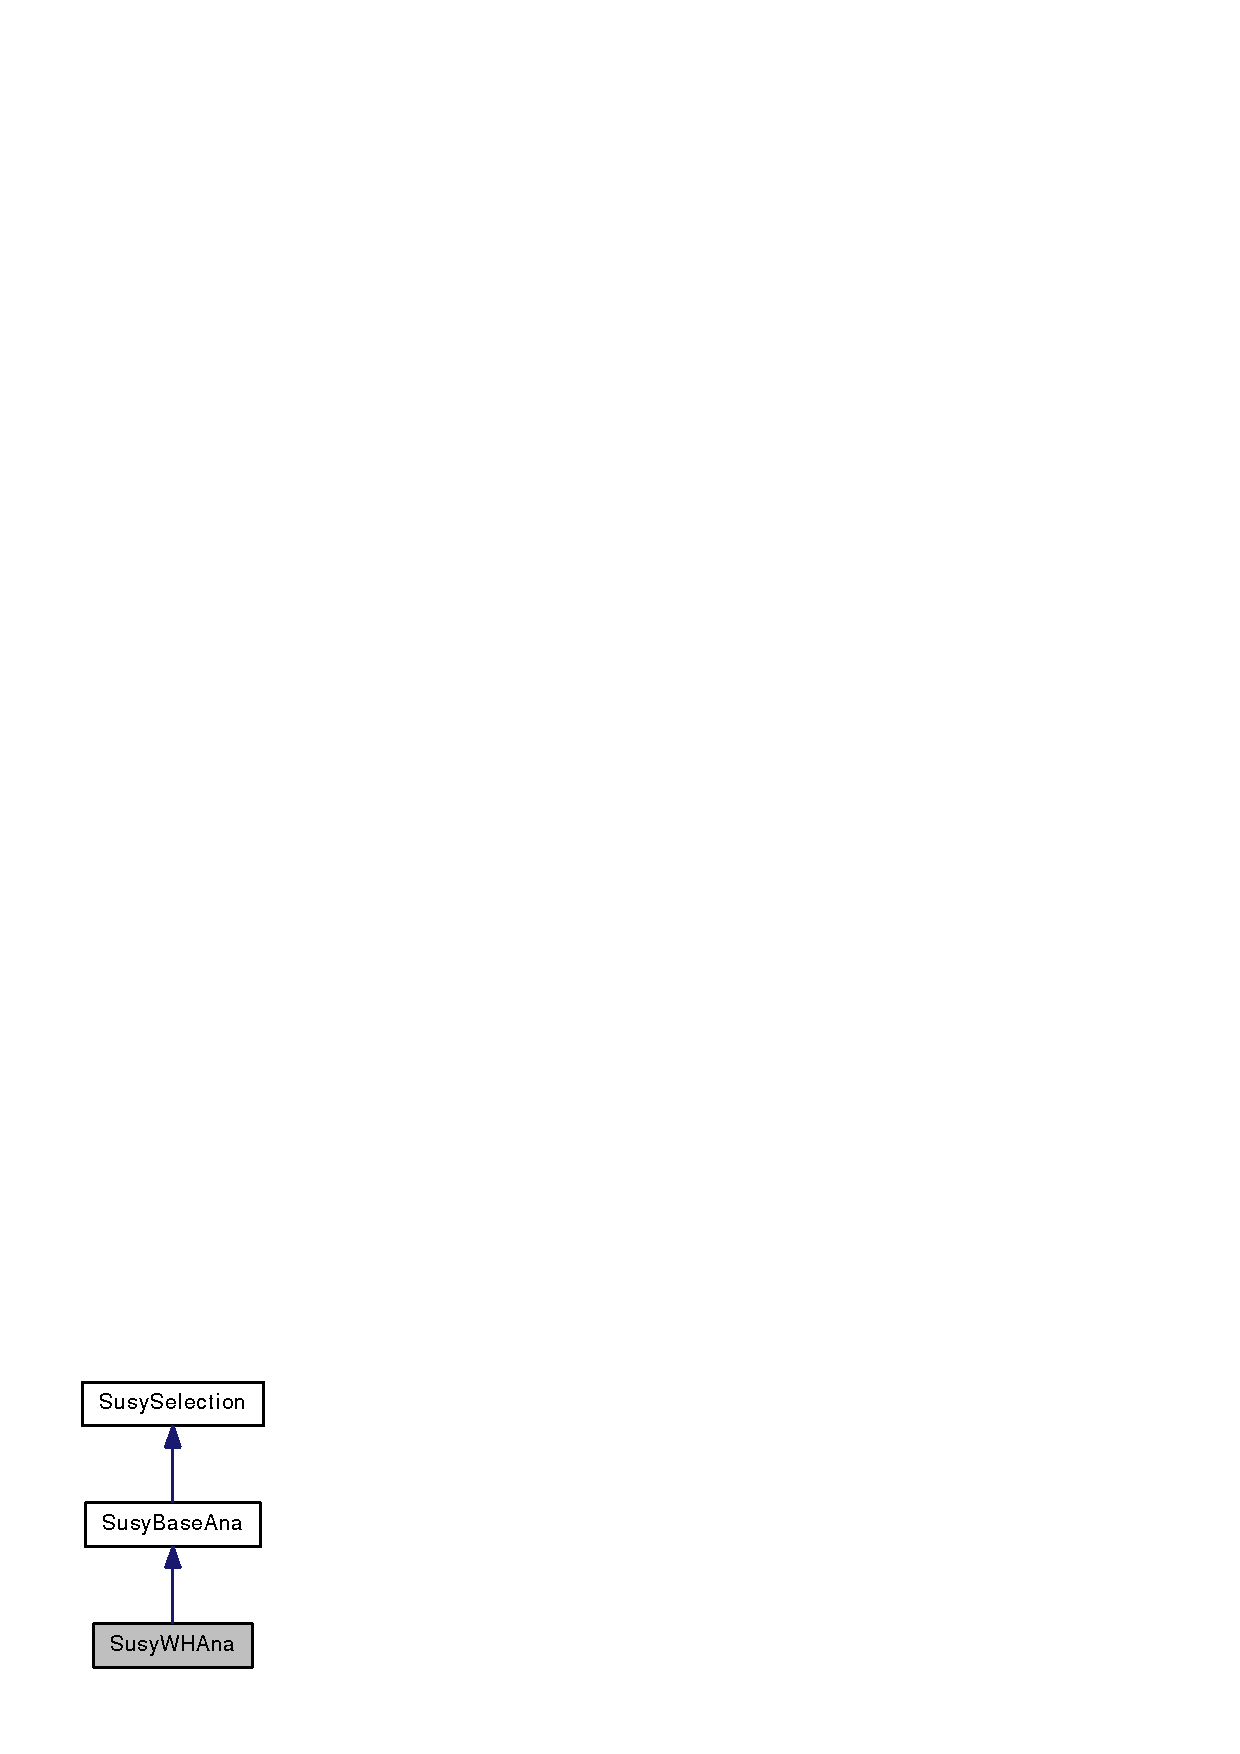
\includegraphics[width=130pt]{classSusyWHAna__inherit__graph}
\end{center}
\end{figure}
Collaboration diagram for SusyWHAna:\nopagebreak
\begin{figure}[H]
\begin{center}
\leavevmode
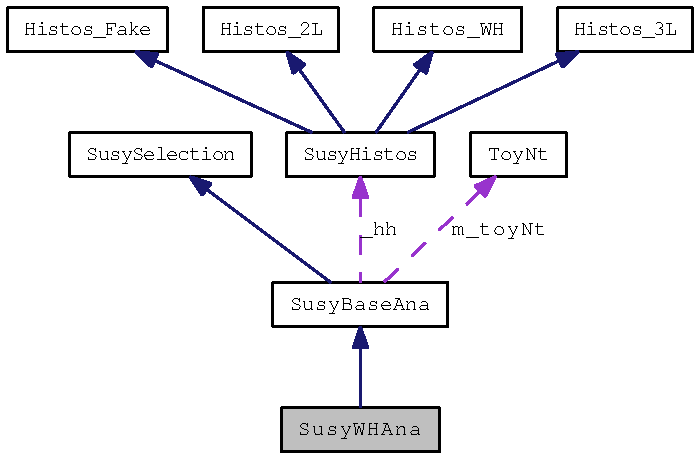
\includegraphics[width=372pt]{classSusyWHAna__coll__graph}
\end{center}
\end{figure}
\subsection*{Public Member Functions}
\begin{DoxyCompactItemize}
\item 
\hypertarget{classSusyWHAna_af63bb9a2a7f0229cf0051cd6b37727b8}{
{\bfseries SusyWHAna} (\hyperlink{classSusyHistos}{SusyHistos} $\ast$\_\-histos)}
\label{classSusyWHAna_af63bb9a2a7f0229cf0051cd6b37727b8}

\item 
\hypertarget{classSusyWHAna_abc1802b72a674ca1958fa2773cdf5efe}{
float {\bfseries getFakeWeight} (const LeptonVector $\ast$leptons, uint nVtx, bool isMC, int iSR, int nJet, float metrel, uint iSys=DGSys\_\-NOM)}
\label{classSusyWHAna_abc1802b72a674ca1958fa2773cdf5efe}

\item 
\hypertarget{classSusyWHAna_a1bd7988df31894a720729a2208e036e4}{
void {\bfseries doAnalysis} (float w, unsigned int isys=DGSys\_\-NOM)}
\label{classSusyWHAna_a1bd7988df31894a720729a2208e036e4}

\item 
\hypertarget{classSusyWHAna_ad93312cf338d21a33d2e72077b2a5757}{
void {\bfseries end} ()}
\label{classSusyWHAna_ad93312cf338d21a33d2e72077b2a5757}

\item 
void \hyperlink{classSusyWHAna_a1926975fddfbbe119c0a6915f303d2db}{setSelection} (std::string s, uint dilType)
\item 
\hypertarget{classSusyWHAna_a370b43f741c46ce2ef2dbb637db837fb}{
bool {\bfseries selectEvent} (LeptonVector $\ast$leptons, LeptonVector $\ast$baseLeptons, const JetVector $\ast$jets, const Met $\ast$met, float \_\-ww)}
\label{classSusyWHAna_a370b43f741c46ce2ef2dbb637db837fb}

\item 
\hypertarget{classSusyWHAna_a2d484e90dc35907e883fc54247b4df7b}{
void {\bfseries fillHistograms} (uint iSR, uint iSYS, const LeptonVector $\ast$leptons, const JetVector $\ast$jets, const Met $\ast$met, float \_\-ww)}
\label{classSusyWHAna_a2d484e90dc35907e883fc54247b4df7b}

\item 
\hypertarget{classSusyWHAna_a8508532b9fc8c2a84dd83bfd6657e683}{
float {\bfseries getWZUncertainty} (uint dsid, int nJet)}
\label{classSusyWHAna_a8508532b9fc8c2a84dd83bfd6657e683}

\item 
\hypertarget{classSusyWHAna_a6d9f2cc6ae4edb2c8290ab3112b10540}{
void {\bfseries print\_\-SRSS} ()}
\label{classSusyWHAna_a6d9f2cc6ae4edb2c8290ab3112b10540}

\item 
\hypertarget{classSusyWHAna_a155b8f95f3d8c8ce14933129cdd58480}{
void {\bfseries print\_\-CRSS} ()}
\label{classSusyWHAna_a155b8f95f3d8c8ce14933129cdd58480}

\item 
\hypertarget{classSusyWHAna_a5289968dd681215f8f3bb9ba975bd302}{
void {\bfseries print\_\-SROSOF2jets} ()}
\label{classSusyWHAna_a5289968dd681215f8f3bb9ba975bd302}

\item 
\hypertarget{classSusyWHAna_a060c861b62071dd24b5f85fac1539b97}{
void {\bfseries print\_\-optimSR} ()}
\label{classSusyWHAna_a060c861b62071dd24b5f85fac1539b97}

\item 
\hypertarget{classSusyWHAna_a17e48f55353ffeddb37505c6848c6c27}{
void {\bfseries print\_\-SRZb} ()}
\label{classSusyWHAna_a17e48f55353ffeddb37505c6848c6c27}

\item 
\hypertarget{classSusyWHAna_a19758f57b6764595aa634edbf4849dde}{
{\bfseries ClassDef} (\hyperlink{classSusyWHAna}{SusyWHAna}, 1)}
\label{classSusyWHAna_a19758f57b6764595aa634edbf4849dde}

\end{DoxyCompactItemize}


\subsection{Member Function Documentation}
\hypertarget{classSusyWHAna_a1926975fddfbbe119c0a6915f303d2db}{
\index{SusyWHAna@{SusyWHAna}!setSelection@{setSelection}}
\index{setSelection@{setSelection}!SusyWHAna@{SusyWHAna}}
\subsubsection[{setSelection}]{\setlength{\rightskip}{0pt plus 5cm}void SusyWHAna::setSelection (std::string {\em s}, \/  uint {\em dilType})}}
\label{classSusyWHAna_a1926975fddfbbe119c0a6915f303d2db}


ZV enriched ! 

The documentation for this class was generated from the following files:\begin{DoxyCompactItemize}
\item 
SusyWeakProdAna/SusyWHAna.h\item 
Root/SusyWHAna.cxx\end{DoxyCompactItemize}

\hypertarget{classToyNt}{
\section{ToyNt Class Reference}
\label{classToyNt}\index{ToyNt@{ToyNt}}
}
\subsection*{Public Member Functions}
\begin{DoxyCompactItemize}
\item 
\hypertarget{classToyNt_ac5182614e93549a4771f0455d5afd895}{
{\bfseries ToyNt} (TString MCID, TString suffix)}
\label{classToyNt_ac5182614e93549a4771f0455d5afd895}

\item 
\hypertarget{classToyNt_abbfd75eca96ec2c41498f7c86f98931f}{
void {\bfseries setBlocks} (bool metD=false, bool dijetB=false, bool OS2LB=false, bool SS2LB=false, bool ZBalB=false, bool diverVarsB=false, bool fakeB=false)}
\label{classToyNt_abbfd75eca96ec2c41498f7c86f98931f}

\item 
\hypertarget{classToyNt_a72ed3a78d77c5306c29566212fbc5d03}{
void {\bfseries BookTree} ()}
\label{classToyNt_a72ed3a78d77c5306c29566212fbc5d03}

\item 
\hypertarget{classToyNt_a619974752eeec49d1f6443630fa4012e}{
void {\bfseries WriteTree} ()}
\label{classToyNt_a619974752eeec49d1f6443630fa4012e}

\item 
\hypertarget{classToyNt_a8a806b704669ab7f065e0c60b8854446}{
void {\bfseries SaveTree} ()}
\label{classToyNt_a8a806b704669ab7f065e0c60b8854446}

\item 
\hypertarget{classToyNt_a598244a544cf7bfedfcee3bed7c89b25}{
void {\bfseries setSumOfMcWeights} (double sumOfMcWeights)}
\label{classToyNt_a598244a544cf7bfedfcee3bed7c89b25}

\item 
\hypertarget{classToyNt_a316cf21d8918dea324e0edc7f4dcebf9}{
string {\bfseries getFilename} () const }
\label{classToyNt_a316cf21d8918dea324e0edc7f4dcebf9}

\item 
\hypertarget{classToyNt_a34261ab251c209f19ebf2d4a003d975c}{
void {\bfseries FillTreeEvent} (int run, int event, int mcId, float npv, float npvCorr, double w, double wbtag, double wqflip)}
\label{classToyNt_a34261ab251c209f19ebf2d4a003d975c}

\item 
\hypertarget{classToyNt_a2de45d19177c47a717f71ecf064d1571}{
void {\bfseries FillTreeLeptons} (const LeptonVector $\ast$leptons, ElectronVector \&baseElectrons, MuonVector \&baseMuons, const Met $\ast$met, int nVtx, bool isMc, int llType)}
\label{classToyNt_a2de45d19177c47a717f71ecf064d1571}

\item 
\hypertarget{classToyNt_aa3966cddb1d0abf0d22e56e9610cf2fa}{
void {\bfseries FillTreeSignalJets} (const JetVector $\ast$jets, const LeptonVector $\ast$leptons, const Met $\ast$met, const ElectronVector $\ast$preElectrons, const MuonVector $\ast$preMuons)}
\label{classToyNt_aa3966cddb1d0abf0d22e56e9610cf2fa}

\item 
\hypertarget{classToyNt_a7e9d50056c5d3826b69272e24a94b015}{
void {\bfseries FillTreeMetVar} (const Met $\ast$met, float metrel)}
\label{classToyNt_a7e9d50056c5d3826b69272e24a94b015}

\item 
\hypertarget{classToyNt_ac05e4e456c358ef4492d7d2597a5856d}{
void {\bfseries FillTreeEventVar} (float mlj, float mljj, float sphericity, float sphericityTrans, float llAcoplanarity, float jjAcoplanarity, bool topTag, float mllCollApprox)}
\label{classToyNt_ac05e4e456c358ef4492d7d2597a5856d}

\item 
\hypertarget{classToyNt_a7983dd33fbd375004e76ef9fb2eb58bc}{
void {\bfseries FillMT2} (float mT2, float mT2jj, float mT2J)}
\label{classToyNt_a7983dd33fbd375004e76ef9fb2eb58bc}

\item 
\hypertarget{classToyNt_ac11708b58e968f49d1da2c5131c805cf}{
void {\bfseries FillMCT} (float mct, float mctPerp, float mctPara)}
\label{classToyNt_ac11708b58e968f49d1da2c5131c805cf}

\item 
\hypertarget{classToyNt_a7230d72a678204257dbd8ff3ab7b4429}{
void {\bfseries FillJZB} (float JZBjets, float JZBmet)}
\label{classToyNt_a7230d72a678204257dbd8ff3ab7b4429}

\item 
\hypertarget{classToyNt_a64e7b0fed4fa2faac2b08d5b845019e5}{
void {\bfseries FillTreeOtherJets} (JetVector $\ast$jets, const LeptonVector $\ast$leptons, const Met $\ast$met)}
\label{classToyNt_a64e7b0fed4fa2faac2b08d5b845019e5}

\item 
\hypertarget{classToyNt_a0b5165d43202460ac67b799aa05ba9fb}{
void {\bfseries findRecoilJet} ()}
\label{classToyNt_a0b5165d43202460ac67b799aa05ba9fb}

\item 
\hypertarget{classToyNt_a52ed26212ca64ba2d16883fb91a0a90e}{
void {\bfseries FillTreeFakeLeptons} (const LeptonVector $\ast$leptons, ElectronVector \&baseElectrons, MuonVector \&baseMuons, const Met $\ast$met, int nVtx, bool isMc)}
\label{classToyNt_a52ed26212ca64ba2d16883fb91a0a90e}

\end{DoxyCompactItemize}
\subsection*{Public Attributes}
\begin{DoxyCompactItemize}
\item 
\hypertarget{classToyNt_a5a7560b824c6550a475641e41c101821}{
bool {\bfseries metDetails}}
\label{classToyNt_a5a7560b824c6550a475641e41c101821}

\item 
\hypertarget{classToyNt_ad92b641c4c6cbbce0c7d8bbc1928b8c7}{
bool {\bfseries dijetBlock}}
\label{classToyNt_ad92b641c4c6cbbce0c7d8bbc1928b8c7}

\item 
\hypertarget{classToyNt_a96b959146f4defe190c35a7cdcfba6e2}{
bool {\bfseries OS2LBlock}}
\label{classToyNt_a96b959146f4defe190c35a7cdcfba6e2}

\item 
\hypertarget{classToyNt_aaeede8b092bc0863d282fd3e1d25bf8e}{
bool {\bfseries SS2LBlock}}
\label{classToyNt_aaeede8b092bc0863d282fd3e1d25bf8e}

\item 
\hypertarget{classToyNt_a1d6db49285909754914c32058957bc81}{
bool {\bfseries ZBalanceBlock}}
\label{classToyNt_a1d6db49285909754914c32058957bc81}

\item 
\hypertarget{classToyNt_a6dff2584128a975e83d511abe181e7f3}{
bool {\bfseries diversVarsBlock}}
\label{classToyNt_a6dff2584128a975e83d511abe181e7f3}

\item 
\hypertarget{classToyNt_a3bfd074ac07ddc435b99e30a3359612f}{
bool {\bfseries fakeBlock}}
\label{classToyNt_a3bfd074ac07ddc435b99e30a3359612f}

\item 
\hypertarget{classToyNt_a3ebba73519c49cfa320fb82677f652ec}{
int {\bfseries \_\-b\_\-run}}
\label{classToyNt_a3ebba73519c49cfa320fb82677f652ec}

\item 
\hypertarget{classToyNt_a17a8af839a2544b726fc12b041d6888f}{
int {\bfseries \_\-b\_\-event}}
\label{classToyNt_a17a8af839a2544b726fc12b041d6888f}

\item 
\hypertarget{classToyNt_ab7d8dfba1b9bdd70519743e113a711a3}{
int {\bfseries \_\-b\_\-mcId}}
\label{classToyNt_ab7d8dfba1b9bdd70519743e113a711a3}

\item 
\hypertarget{classToyNt_a987e15d3493974719d26878a7249f9c1}{
float {\bfseries \_\-b\_\-npv}}
\label{classToyNt_a987e15d3493974719d26878a7249f9c1}

\item 
\hypertarget{classToyNt_adacf50a8d7dd0a05a82dde429432d0b9}{
float {\bfseries \_\-b\_\-npvCorr}}
\label{classToyNt_adacf50a8d7dd0a05a82dde429432d0b9}

\item 
\hypertarget{classToyNt_a0ad4c1344adf448ce9962d6d6fa24a8e}{
double {\bfseries \_\-b\_\-w}}
\label{classToyNt_a0ad4c1344adf448ce9962d6d6fa24a8e}

\item 
\hypertarget{classToyNt_a5df379cce2c784c58d97386ce64e2a3f}{
double {\bfseries \_\-b\_\-wbtag}}
\label{classToyNt_a5df379cce2c784c58d97386ce64e2a3f}

\item 
\hypertarget{classToyNt_aeec0ae0072e5aef0025f86c98723b482}{
double {\bfseries \_\-b\_\-wqflip}}
\label{classToyNt_aeec0ae0072e5aef0025f86c98723b482}

\item 
\hypertarget{classToyNt_a50198335a69fa72e7c7da9c087b0e980}{
int {\bfseries \_\-b\_\-nlep}}
\label{classToyNt_a50198335a69fa72e7c7da9c087b0e980}

\item 
\hypertarget{classToyNt_ae5854ff7cd45c8a0399f91791e05a963}{
float {\bfseries \_\-b\_\-l\_\-pt} \mbox{[}nLepMax\mbox{]}}
\label{classToyNt_ae5854ff7cd45c8a0399f91791e05a963}

\item 
\hypertarget{classToyNt_a75c9065228884135ba03a07a3f20eca9}{
float {\bfseries \_\-b\_\-l\_\-eta} \mbox{[}nLepMax\mbox{]}}
\label{classToyNt_a75c9065228884135ba03a07a3f20eca9}

\item 
\hypertarget{classToyNt_a4759843f452b3de69269c45214367f01}{
float {\bfseries \_\-b\_\-l\_\-phi} \mbox{[}nLepMax\mbox{]}}
\label{classToyNt_a4759843f452b3de69269c45214367f01}

\item 
\hypertarget{classToyNt_ab7384ceeb491342578ef35640a3f051b}{
float {\bfseries \_\-b\_\-l\_\-e} \mbox{[}nLepMax\mbox{]}}
\label{classToyNt_ab7384ceeb491342578ef35640a3f051b}

\item 
\hypertarget{classToyNt_a9a5dd10d3b10a98f25202ca3e6cfdf5e}{
float {\bfseries \_\-b\_\-l\_\-Y} \mbox{[}nLepMax\mbox{]}}
\label{classToyNt_a9a5dd10d3b10a98f25202ca3e6cfdf5e}

\item 
\hypertarget{classToyNt_ae77cbc54d0c46c41e755852f3b6e2791}{
int {\bfseries \_\-b\_\-l\_\-q} \mbox{[}nLepMax\mbox{]}}
\label{classToyNt_ae77cbc54d0c46c41e755852f3b6e2791}

\item 
\hypertarget{classToyNt_a7026079f20f2910cdc93830a325f737c}{
float {\bfseries \_\-b\_\-l\_\-ptcone30} \mbox{[}nLepMax\mbox{]}}
\label{classToyNt_a7026079f20f2910cdc93830a325f737c}

\item 
\hypertarget{classToyNt_a525b198ec1dcbe910a416e943b46c6cb}{
float {\bfseries \_\-b\_\-l\_\-etcone30} \mbox{[}nLepMax\mbox{]}}
\label{classToyNt_a525b198ec1dcbe910a416e943b46c6cb}

\item 
\hypertarget{classToyNt_aebb63953d8693051cfb4478b6210bd01}{
float {\bfseries \_\-b\_\-l\_\-etconetopo30} \mbox{[}nLepMax\mbox{]}}
\label{classToyNt_aebb63953d8693051cfb4478b6210bd01}

\item 
\hypertarget{classToyNt_a43c2bbfa347a2679b9541c100b6f9503}{
float {\bfseries \_\-b\_\-l\_\-d0} \mbox{[}nLepMax\mbox{]}}
\label{classToyNt_a43c2bbfa347a2679b9541c100b6f9503}

\item 
\hypertarget{classToyNt_ab039c8f8b81db172d99bebea84a2bf06}{
float {\bfseries \_\-b\_\-l\_\-d0Err} \mbox{[}nLepMax\mbox{]}}
\label{classToyNt_ab039c8f8b81db172d99bebea84a2bf06}

\item 
\hypertarget{classToyNt_aa57fe54ec1fc669193f8d11acdcfbcb9}{
float {\bfseries \_\-b\_\-l\_\-z0} \mbox{[}nLepMax\mbox{]}}
\label{classToyNt_aa57fe54ec1fc669193f8d11acdcfbcb9}

\item 
\hypertarget{classToyNt_ad9fff30ecda0091b61add06cd80c6b04}{
bool {\bfseries \_\-b\_\-l\_\-isEle} \mbox{[}nLepMax\mbox{]}}
\label{classToyNt_ad9fff30ecda0091b61add06cd80c6b04}

\item 
\hypertarget{classToyNt_a97c6a2354b45a8206a405928d5e41fc2}{
bool {\bfseries \_\-b\_\-l\_\-isT} \mbox{[}nLepMax\mbox{]}}
\label{classToyNt_a97c6a2354b45a8206a405928d5e41fc2}

\item 
\hypertarget{classToyNt_a6f57818e97989400205ea2372abdc091}{
int {\bfseries \_\-b\_\-l\_\-org} \mbox{[}nLepMax\mbox{]}}
\label{classToyNt_a6f57818e97989400205ea2372abdc091}

\item 
\hypertarget{classToyNt_adfc600a2b858a46bd0f601318d6cf1b9}{
bool {\bfseries \_\-b\_\-l\_\-isQFlip} \mbox{[}nLepMax\mbox{]}}
\label{classToyNt_adfc600a2b858a46bd0f601318d6cf1b9}

\item 
\hypertarget{classToyNt_a4e26f4f4d4c39e781319be6fc432c526}{
bool {\bfseries \_\-b\_\-isOS}}
\label{classToyNt_a4e26f4f4d4c39e781319be6fc432c526}

\item 
\hypertarget{classToyNt_aaa94f04aae09b6b13dc10618ad4f0afc}{
bool {\bfseries \_\-b\_\-isGenuineSS}}
\label{classToyNt_aaa94f04aae09b6b13dc10618ad4f0afc}

\item 
\hypertarget{classToyNt_ab3b731b9fd2ef20162789166144637f5}{
int {\bfseries \_\-b\_\-llType}}
\label{classToyNt_ab3b731b9fd2ef20162789166144637f5}

\item 
\hypertarget{classToyNt_a1cc05ee5b235bce7363cc85a2f579ec8}{
float {\bfseries \_\-b\_\-dphi\_\-ll}}
\label{classToyNt_a1cc05ee5b235bce7363cc85a2f579ec8}

\item 
\hypertarget{classToyNt_a0eab51b74f43b656f50e804ed6718621}{
float {\bfseries \_\-b\_\-deta\_\-ll}}
\label{classToyNt_a0eab51b74f43b656f50e804ed6718621}

\item 
\hypertarget{classToyNt_af5aa6b75df7e0528717c1efc56b90606}{
float {\bfseries \_\-b\_\-dR\_\-ll}}
\label{classToyNt_af5aa6b75df7e0528717c1efc56b90606}

\item 
\hypertarget{classToyNt_a4902a43dc45740a02fb50cf317f0abac}{
float {\bfseries \_\-b\_\-pTll}}
\label{classToyNt_a4902a43dc45740a02fb50cf317f0abac}

\item 
\hypertarget{classToyNt_add0fa1fcf17d67057ed2323f17567faa}{
float {\bfseries \_\-b\_\-phill}}
\label{classToyNt_add0fa1fcf17d67057ed2323f17567faa}

\item 
\hypertarget{classToyNt_a4606e3902c7f3ebf41a7dee893d1475d}{
float {\bfseries \_\-b\_\-mll}}
\label{classToyNt_a4606e3902c7f3ebf41a7dee893d1475d}

\item 
\hypertarget{classToyNt_a6b1b87dc3410af0c508d8bdaf3309f1f}{
float {\bfseries \_\-b\_\-mll\_\-collApprox}}
\label{classToyNt_a6b1b87dc3410af0c508d8bdaf3309f1f}

\item 
\hypertarget{classToyNt_a2402c8c2aff0d9025a5a08f25d3177f8}{
float {\bfseries \_\-b\_\-dphi\_\-ll\_\-j1}}
\label{classToyNt_a2402c8c2aff0d9025a5a08f25d3177f8}

\item 
\hypertarget{classToyNt_a01a43887f9ed1898f1a6eb1e6f02e582}{
float {\bfseries \_\-b\_\-met}}
\label{classToyNt_a01a43887f9ed1898f1a6eb1e6f02e582}

\item 
\hypertarget{classToyNt_a9c33c48f116e1afed766c8cac55af318}{
float {\bfseries \_\-b\_\-met\_\-phi}}
\label{classToyNt_a9c33c48f116e1afed766c8cac55af318}

\item 
\hypertarget{classToyNt_a9844f7988361655b33cb68e369215348}{
float {\bfseries \_\-b\_\-metrel}}
\label{classToyNt_a9844f7988361655b33cb68e369215348}

\item 
\hypertarget{classToyNt_a369aeadcec6c286e23ad9887762ad598}{
float {\bfseries \_\-b\_\-met\_\-refEle}}
\label{classToyNt_a369aeadcec6c286e23ad9887762ad598}

\item 
\hypertarget{classToyNt_a9c9d444de1fe149f026b4f48bcb26e76}{
float {\bfseries \_\-b\_\-met\_\-refMuo}}
\label{classToyNt_a9c9d444de1fe149f026b4f48bcb26e76}

\item 
\hypertarget{classToyNt_afbb0e1c525bfd9c19da8a9348c9b2433}{
float {\bfseries \_\-b\_\-met\_\-refJet}}
\label{classToyNt_afbb0e1c525bfd9c19da8a9348c9b2433}

\item 
\hypertarget{classToyNt_adc97f8ac8be3bf7700c5a38227d92d54}{
float {\bfseries \_\-b\_\-met\_\-cellout}}
\label{classToyNt_adc97f8ac8be3bf7700c5a38227d92d54}

\item 
\hypertarget{classToyNt_ae08c9ee5922ee0a97165174088e08488}{
int {\bfseries \_\-b\_\-nJets}}
\label{classToyNt_ae08c9ee5922ee0a97165174088e08488}

\item 
\hypertarget{classToyNt_aa9c9f99aa30ae0ff19ea6e37b8aeaa7e}{
int {\bfseries \_\-b\_\-nSJets}}
\label{classToyNt_aa9c9f99aa30ae0ff19ea6e37b8aeaa7e}

\item 
\hypertarget{classToyNt_acb132a28446e60a308982acc944b5b88}{
int {\bfseries \_\-b\_\-nCJets}}
\label{classToyNt_acb132a28446e60a308982acc944b5b88}

\item 
\hypertarget{classToyNt_acdc34ec5c7528d565ac0126f17f0f7d8}{
int {\bfseries \_\-b\_\-nBJets}}
\label{classToyNt_acdc34ec5c7528d565ac0126f17f0f7d8}

\item 
\hypertarget{classToyNt_aa211b880febab89e7a2c454ccc6b1273}{
int {\bfseries \_\-b\_\-nFJets}}
\label{classToyNt_aa211b880febab89e7a2c454ccc6b1273}

\item 
\hypertarget{classToyNt_a2aa9eadd9d9626ad8e76d797aec53fa2}{
bool {\bfseries \_\-b\_\-j\_\-isC20} \mbox{[}25\mbox{]}}
\label{classToyNt_a2aa9eadd9d9626ad8e76d797aec53fa2}

\item 
\hypertarget{classToyNt_a8cd86501883824bd156f083ecb6c98d0}{
bool {\bfseries \_\-b\_\-j\_\-isB20} \mbox{[}25\mbox{]}}
\label{classToyNt_a8cd86501883824bd156f083ecb6c98d0}

\item 
\hypertarget{classToyNt_a1cf48698d381f2b95d5364ae870407b5}{
bool {\bfseries \_\-b\_\-j\_\-isF30} \mbox{[}25\mbox{]}}
\label{classToyNt_a1cf48698d381f2b95d5364ae870407b5}

\item 
\hypertarget{classToyNt_ae1f54b70286bacacfd15edf6f9aef049}{
float {\bfseries \_\-b\_\-j\_\-pt} \mbox{[}25\mbox{]}}
\label{classToyNt_ae1f54b70286bacacfd15edf6f9aef049}

\item 
\hypertarget{classToyNt_aee080f93ec3def59a098f571099076b0}{
float {\bfseries \_\-b\_\-j\_\-eta} \mbox{[}25\mbox{]}}
\label{classToyNt_aee080f93ec3def59a098f571099076b0}

\item 
\hypertarget{classToyNt_a57e7ce06a5462264df6f31b63627b546}{
float {\bfseries \_\-b\_\-j\_\-phi} \mbox{[}25\mbox{]}}
\label{classToyNt_a57e7ce06a5462264df6f31b63627b546}

\item 
\hypertarget{classToyNt_a3b00b4de17e1aee736d7f87d63b3bfda}{
float {\bfseries \_\-b\_\-j\_\-e} \mbox{[}25\mbox{]}}
\label{classToyNt_a3b00b4de17e1aee736d7f87d63b3bfda}

\item 
\hypertarget{classToyNt_ada81af13a486e0d88610c49478b95483}{
float {\bfseries \_\-b\_\-j\_\-Y} \mbox{[}25\mbox{]}}
\label{classToyNt_ada81af13a486e0d88610c49478b95483}

\item 
\hypertarget{classToyNt_af861f0b541cd0c34b3e05767ac47c4af}{
float {\bfseries \_\-b\_\-j\_\-jvf} \mbox{[}25\mbox{]}}
\label{classToyNt_af861f0b541cd0c34b3e05767ac47c4af}

\item 
\hypertarget{classToyNt_a39ea60160a05dcf278b948b675a31b1e}{
float {\bfseries \_\-b\_\-j\_\-mv1} \mbox{[}25\mbox{]}}
\label{classToyNt_a39ea60160a05dcf278b948b675a31b1e}

\item 
\hypertarget{classToyNt_aab5fb4ed4056efacf601c3230e19cb08}{
int {\bfseries \_\-b\_\-j\_\-nEle} \mbox{[}25\mbox{]}}
\label{classToyNt_aab5fb4ed4056efacf601c3230e19cb08}

\item 
\hypertarget{classToyNt_aab0a261376966245128245154fa943ef}{
int {\bfseries \_\-b\_\-j\_\-nMu} \mbox{[}25\mbox{]}}
\label{classToyNt_aab0a261376966245128245154fa943ef}

\item 
\hypertarget{classToyNt_a81979409a45025b7fda3b0bb613f75ca}{
bool {\bfseries \_\-b\_\-j\_\-isTruth} \mbox{[}25\mbox{]}}
\label{classToyNt_a81979409a45025b7fda3b0bb613f75ca}

\item 
\hypertarget{classToyNt_a5796781f716e1d495d0962b1cc457e31}{
int {\bfseries \_\-b\_\-j\_\-label} \mbox{[}25\mbox{]}}
\label{classToyNt_a5796781f716e1d495d0962b1cc457e31}

\item 
\hypertarget{classToyNt_a7d7617c2424b62aea09c8a4745636c2c}{
float {\bfseries \_\-b\_\-mEff}}
\label{classToyNt_a7d7617c2424b62aea09c8a4745636c2c}

\item 
\hypertarget{classToyNt_ae1bb719cda265cb38ba1419df6a17c87}{
float {\bfseries \_\-b\_\-ST}}
\label{classToyNt_ae1bb719cda265cb38ba1419df6a17c87}

\item 
\hypertarget{classToyNt_a7a72aada85c3e70fe4d0e56d4a11fdb1}{
bool {\bfseries \_\-b\_\-topTag}}
\label{classToyNt_a7a72aada85c3e70fe4d0e56d4a11fdb1}

\item 
\hypertarget{classToyNt_a8ddd77465abcb726db93cdc8c4436d96}{
float {\bfseries \_\-b\_\-dphi\_\-metl} \mbox{[}nLepMax\mbox{]}}
\label{classToyNt_a8ddd77465abcb726db93cdc8c4436d96}

\item 
\hypertarget{classToyNt_a574969f5275c08f9ee3d27e4024e444e}{
float {\bfseries \_\-b\_\-mTl} \mbox{[}nLepMax\mbox{]}}
\label{classToyNt_a574969f5275c08f9ee3d27e4024e444e}

\item 
\hypertarget{classToyNt_a6b637e1afc3691d74f7fce8e4357d907}{
float {\bfseries \_\-b\_\-dphi\_\-metcl}}
\label{classToyNt_a6b637e1afc3691d74f7fce8e4357d907}

\item 
\hypertarget{classToyNt_a6ac7de97bad28fe69f64a9a53e308035}{
float {\bfseries \_\-b\_\-dphi\_\-metcj}}
\label{classToyNt_a6ac7de97bad28fe69f64a9a53e308035}

\item 
\hypertarget{classToyNt_abb0fb36d0b3839437c3593e99087e448}{
float {\bfseries \_\-b\_\-mjj}}
\label{classToyNt_abb0fb36d0b3839437c3593e99087e448}

\item 
\hypertarget{classToyNt_abc17a93dda64c8c9f59754f8b706b735}{
float {\bfseries \_\-b\_\-pTjj}}
\label{classToyNt_abc17a93dda64c8c9f59754f8b706b735}

\item 
\hypertarget{classToyNt_a5da467ae40f499cb5190598c3cb7fbc4}{
float {\bfseries \_\-b\_\-dRjj}}
\label{classToyNt_a5da467ae40f499cb5190598c3cb7fbc4}

\item 
\hypertarget{classToyNt_ac65601d6327e34270012e8dbe5029053}{
float {\bfseries \_\-b\_\-dEtajj}}
\label{classToyNt_ac65601d6327e34270012e8dbe5029053}

\item 
\hypertarget{classToyNt_adea2b1de0540c57e74b761eaf13fd563}{
float {\bfseries \_\-b\_\-mT2}}
\label{classToyNt_adea2b1de0540c57e74b761eaf13fd563}

\item 
\hypertarget{classToyNt_af44bb109f2b83e7e61f9d75718473bcb}{
float {\bfseries \_\-b\_\-mT2jj}}
\label{classToyNt_af44bb109f2b83e7e61f9d75718473bcb}

\item 
\hypertarget{classToyNt_a85285c2ce770a2d4ef96a9886e782757}{
float {\bfseries \_\-b\_\-mT2J}}
\label{classToyNt_a85285c2ce770a2d4ef96a9886e782757}

\item 
\hypertarget{classToyNt_adcc0dd20b56ea7f0ca00df199c4e87c9}{
float {\bfseries \_\-b\_\-mct}}
\label{classToyNt_adcc0dd20b56ea7f0ca00df199c4e87c9}

\item 
\hypertarget{classToyNt_a09351459ed578a9003245352f5f93c9f}{
float {\bfseries \_\-b\_\-mctPerp}}
\label{classToyNt_a09351459ed578a9003245352f5f93c9f}

\item 
\hypertarget{classToyNt_a0598a8d19b13e21f40e11d5f24583b7e}{
float {\bfseries \_\-b\_\-mctPara}}
\label{classToyNt_a0598a8d19b13e21f40e11d5f24583b7e}

\item 
\hypertarget{classToyNt_ad7dcc7b110c49d7dd562f21d8159704e}{
float {\bfseries \_\-b\_\-mWWT}}
\label{classToyNt_ad7dcc7b110c49d7dd562f21d8159704e}

\item 
\hypertarget{classToyNt_a9f3c359c269271308d1e5bf90da7830b}{
float {\bfseries \_\-b\_\-mlj}}
\label{classToyNt_a9f3c359c269271308d1e5bf90da7830b}

\item 
\hypertarget{classToyNt_a93b14688f40c4cc84916982829922d17}{
float {\bfseries \_\-b\_\-mljj}}
\label{classToyNt_a93b14688f40c4cc84916982829922d17}

\item 
\hypertarget{classToyNt_a94119ed602c247352b0a39a5e149f38f}{
int {\bfseries \_\-b\_\-nOJets}}
\label{classToyNt_a94119ed602c247352b0a39a5e149f38f}

\item 
\hypertarget{classToyNt_a6eb70804fdbba2aeeb5c55ed5d5913db}{
bool {\bfseries \_\-b\_\-j\_\-isOJ} \mbox{[}25\mbox{]}}
\label{classToyNt_a6eb70804fdbba2aeeb5c55ed5d5913db}

\item 
\hypertarget{classToyNt_ae1f7d6dfe6bd5ff41d35a4474d6d684e}{
bool {\bfseries \_\-b\_\-j\_\-isRecoil} \mbox{[}25\mbox{]}}
\label{classToyNt_ae1f7d6dfe6bd5ff41d35a4474d6d684e}

\item 
\hypertarget{classToyNt_ac2e3b392674a426760cacac7abaa6204}{
bool {\bfseries \_\-b\_\-j\_\-isSublead} \mbox{[}25\mbox{]}}
\label{classToyNt_ac2e3b392674a426760cacac7abaa6204}

\item 
\hypertarget{classToyNt_a20be5d3af210b3227dca5e27bb8f434f}{
float {\bfseries \_\-b\_\-dphi\_\-Zj}}
\label{classToyNt_a20be5d3af210b3227dca5e27bb8f434f}

\item 
\hypertarget{classToyNt_a5802228f75635ff5633d1f62317d4825}{
float {\bfseries \_\-b\_\-dphi\_\-ll\_\-oj1}}
\label{classToyNt_a5802228f75635ff5633d1f62317d4825}

\item 
\hypertarget{classToyNt_abdc894b3f11ade6dd34346c1e2384465}{
float {\bfseries \_\-b\_\-dphi\_\-metcoj}}
\label{classToyNt_abdc894b3f11ade6dd34346c1e2384465}

\item 
\hypertarget{classToyNt_ab75e263d23f9130ba1b066a8860dfa0b}{
float {\bfseries \_\-b\_\-sphericity}}
\label{classToyNt_ab75e263d23f9130ba1b066a8860dfa0b}

\item 
\hypertarget{classToyNt_a06b0134ceb85273e8f27445d70272d8c}{
float {\bfseries \_\-b\_\-sphericityTrans}}
\label{classToyNt_a06b0134ceb85273e8f27445d70272d8c}

\item 
\hypertarget{classToyNt_a1cf64ae61bb3e8c05b594f3a2663ed32}{
float {\bfseries \_\-b\_\-llAcoplanarity}}
\label{classToyNt_a1cf64ae61bb3e8c05b594f3a2663ed32}

\item 
\hypertarget{classToyNt_adfeb7173c1e3237fa5ebfd36383a28b7}{
float {\bfseries \_\-b\_\-jjAcoplanarity}}
\label{classToyNt_adfeb7173c1e3237fa5ebfd36383a28b7}

\item 
\hypertarget{classToyNt_a421838424a9b098d21eb991024a7d8b0}{
float {\bfseries \_\-b\_\-JZBjets}}
\label{classToyNt_a421838424a9b098d21eb991024a7d8b0}

\item 
\hypertarget{classToyNt_a4d2f8e8e64509a262a2c8e50689af37b}{
float {\bfseries \_\-b\_\-JZBmet}}
\label{classToyNt_a4d2f8e8e64509a262a2c8e50689af37b}

\item 
\hypertarget{classToyNt_ac6f2ff79c059048171a19ff80913b4dc}{
float {\bfseries \_\-b\_\-pTll\_\-Tb}}
\label{classToyNt_ac6f2ff79c059048171a19ff80913b4dc}

\item 
\hypertarget{classToyNt_a77acc076c14280170b0dc8e8724bdb08}{
float {\bfseries \_\-b\_\-dPhib}}
\label{classToyNt_a77acc076c14280170b0dc8e8724bdb08}

\item 
\hypertarget{classToyNt_a9cf1d4b85d65fc2bf1339a0de7d9bae7}{
int {\bfseries \_\-b\_\-ll\_\-FType}}
\label{classToyNt_a9cf1d4b85d65fc2bf1339a0de7d9bae7}

\item 
\hypertarget{classToyNt_a2d1b00a94b2b5102245e66d01c4cab82}{
bool {\bfseries \_\-b\_\-pass\_\-SS1j}}
\label{classToyNt_a2d1b00a94b2b5102245e66d01c4cab82}

\item 
\hypertarget{classToyNt_a6485f2574917a3d73748a7d4544ee08c}{
bool {\bfseries \_\-b\_\-pass\_\-SSEM}}
\label{classToyNt_a6485f2574917a3d73748a7d4544ee08c}

\item 
\hypertarget{classToyNt_a6b36b56bd1715b9a4c6f3c7f29108300}{
bool {\bfseries \_\-b\_\-pass\_\-HFTP}}
\label{classToyNt_a6b36b56bd1715b9a4c6f3c7f29108300}

\item 
\hypertarget{classToyNt_a910f40cd2a8443f14677d179555d96ae}{
bool {\bfseries \_\-b\_\-pass\_\-MCEff}}
\label{classToyNt_a910f40cd2a8443f14677d179555d96ae}

\item 
\hypertarget{classToyNt_a258068147da97c4777e7cabccebff7be}{
bool {\bfseries \_\-b\_\-pass\_\-ZTP}}
\label{classToyNt_a258068147da97c4777e7cabccebff7be}

\item 
\hypertarget{classToyNt_ab57f00542717539dd1ff92c9bb134f3a}{
bool {\bfseries \_\-b\_\-pass\_\-ZConv}}
\label{classToyNt_ab57f00542717539dd1ff92c9bb134f3a}

\item 
\hypertarget{classToyNt_a12c2d1d7b9bef427f2ec68c5bc744b8a}{
bool {\bfseries \_\-b\_\-pass\_\-ZHFLF}}
\label{classToyNt_a12c2d1d7b9bef427f2ec68c5bc744b8a}

\item 
\hypertarget{classToyNt_a06bbed0e0f626ad38df3fa0d5d920f2b}{
int {\bfseries \_\-b\_\-SSEM\_\-tagIdx}}
\label{classToyNt_a06bbed0e0f626ad38df3fa0d5d920f2b}

\item 
\hypertarget{classToyNt_af487dc751a6d2be69ccbe4dedcd408d6}{
int {\bfseries \_\-b\_\-SSEM\_\-probeIdx}}
\label{classToyNt_af487dc751a6d2be69ccbe4dedcd408d6}

\item 
\hypertarget{classToyNt_a3bdfdf4cd0dd9e94574386f542368db8}{
int {\bfseries \_\-b\_\-HFTP\_\-tagIdx}}
\label{classToyNt_a3bdfdf4cd0dd9e94574386f542368db8}

\item 
\hypertarget{classToyNt_a412a1fc2c65dd1c5307ed636738c3948}{
int {\bfseries \_\-b\_\-HFTP\_\-probeIdx}}
\label{classToyNt_a412a1fc2c65dd1c5307ed636738c3948}

\item 
\hypertarget{classToyNt_aa8ae5a005fd6b9a4827f45a1ae86edfd}{
int {\bfseries \_\-b\_\-ZTP\_\-tagIdx1}}
\label{classToyNt_aa8ae5a005fd6b9a4827f45a1ae86edfd}

\item 
\hypertarget{classToyNt_a41d69324b7b14663d5fcbc75eb5272b4}{
int {\bfseries \_\-b\_\-ZTP\_\-probeIdx1}}
\label{classToyNt_a41d69324b7b14663d5fcbc75eb5272b4}

\item 
\hypertarget{classToyNt_acdc7ac417623a6e8e17be7ae042e1e4c}{
int {\bfseries \_\-b\_\-ZTP\_\-tagIdx2}}
\label{classToyNt_acdc7ac417623a6e8e17be7ae042e1e4c}

\item 
\hypertarget{classToyNt_a1c95ab572987e63684ef7e10063eea70}{
int {\bfseries \_\-b\_\-ZTP\_\-probeIdx2}}
\label{classToyNt_a1c95ab572987e63684ef7e10063eea70}

\item 
\hypertarget{classToyNt_a764d1273e611b13d75d14ed70fb463b7}{
int {\bfseries \_\-b\_\-ZConv\_\-tagIdx1}}
\label{classToyNt_a764d1273e611b13d75d14ed70fb463b7}

\item 
\hypertarget{classToyNt_a962c255a2faa1b1fc444a2d57a8cb77a}{
int {\bfseries \_\-b\_\-ZConv\_\-tagIdx2}}
\label{classToyNt_a962c255a2faa1b1fc444a2d57a8cb77a}

\item 
\hypertarget{classToyNt_acd67dc82c3ea03e4cb532ede7391f810}{
int {\bfseries \_\-b\_\-ZConv\_\-probeIdx}}
\label{classToyNt_acd67dc82c3ea03e4cb532ede7391f810}

\item 
\hypertarget{classToyNt_a483966e9bb82edebce209097d4532608}{
int {\bfseries \_\-b\_\-ZHFLF\_\-tagIdx1}}
\label{classToyNt_a483966e9bb82edebce209097d4532608}

\item 
\hypertarget{classToyNt_a106431520c859cc798d29fc75aefc014}{
int {\bfseries \_\-b\_\-ZHFLF\_\-tagIdx2}}
\label{classToyNt_a106431520c859cc798d29fc75aefc014}

\item 
\hypertarget{classToyNt_a7f2eb8773c245e2a22a6f8732497047d}{
int {\bfseries \_\-b\_\-ZHFLF\_\-probeIdx}}
\label{classToyNt_a7f2eb8773c245e2a22a6f8732497047d}

\item 
\hypertarget{classToyNt_ad14b0eff6340bb3ca577e02e931d8fad}{
float {\bfseries \_\-b\_\-ZHFLF\_\-mlll}}
\label{classToyNt_ad14b0eff6340bb3ca577e02e931d8fad}

\end{DoxyCompactItemize}
\subsection*{Static Public Attributes}
\begin{DoxyCompactItemize}
\item 
\hypertarget{classToyNt_a307fa091dd1ccae44e90ac71b6b90f4a}{
static const unsigned int {\bfseries nLepMax} = 5}
\label{classToyNt_a307fa091dd1ccae44e90ac71b6b90f4a}

\end{DoxyCompactItemize}


The documentation for this class was generated from the following files:\begin{DoxyCompactItemize}
\item 
SusyWeakProdAna/ToyNt.h\item 
Root/ToyNt.cxx\end{DoxyCompactItemize}

\hypertarget{classToyNt__SROptimization}{
\section{ToyNt\_\-SROptimization Class Reference}
\label{classToyNt__SROptimization}\index{ToyNt\_\-SROptimization@{ToyNt\_\-SROptimization}}
}
Inheritance diagram for ToyNt\_\-SROptimization:\nopagebreak
\begin{figure}[H]
\begin{center}
\leavevmode
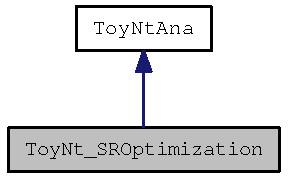
\includegraphics[width=174pt]{classToyNt__SROptimization__inherit__graph}
\end{center}
\end{figure}
Collaboration diagram for ToyNt\_\-SROptimization:\nopagebreak
\begin{figure}[H]
\begin{center}
\leavevmode
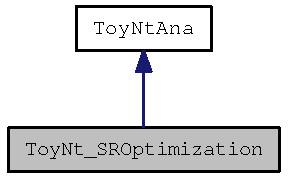
\includegraphics[width=174pt]{classToyNt__SROptimization__coll__graph}
\end{center}
\end{figure}
\subsection*{Public Member Functions}
\begin{DoxyCompactItemize}
\item 
\hypertarget{classToyNt__SROptimization_adecb5beed52cb945815df2dc9c32d8ca}{
virtual void {\bfseries Begin} (TTree $\ast$tree)}
\label{classToyNt__SROptimization_adecb5beed52cb945815df2dc9c32d8ca}

\item 
\hypertarget{classToyNt__SROptimization_ad4cf1cfac6e5036a094b0bd1f926cc1b}{
virtual void {\bfseries Terminate} ()}
\label{classToyNt__SROptimization_ad4cf1cfac6e5036a094b0bd1f926cc1b}

\item 
\hypertarget{classToyNt__SROptimization_abbee1b8c437ee05569960f94c8d9579e}{
virtual Bool\_\-t {\bfseries Process} (Long64\_\-t entry)}
\label{classToyNt__SROptimization_abbee1b8c437ee05569960f94c8d9579e}

\item 
\hypertarget{classToyNt__SROptimization_a415f4471f18d5632962648a0f5f28fc5}{
void {\bfseries Analyze} ()}
\label{classToyNt__SROptimization_a415f4471f18d5632962648a0f5f28fc5}

\item 
\hypertarget{classToyNt__SROptimization_a1facd6744048c4519bd242e1d9440eb2}{
void {\bfseries PrintInfo} ()}
\label{classToyNt__SROptimization_a1facd6744048c4519bd242e1d9440eb2}

\item 
\hypertarget{classToyNt__SROptimization_a0c19731d8fc24a81fefc0be74c75ce34}{
{\bfseries ClassDef} (\hyperlink{classToyNt__SROptimization}{ToyNt\_\-SROptimization}, 1)}
\label{classToyNt__SROptimization_a0c19731d8fc24a81fefc0be74c75ce34}

\end{DoxyCompactItemize}
\subsection*{Public Attributes}
\begin{DoxyCompactItemize}
\item 
\hypertarget{classToyNt__SROptimization_a51de9284d40de871db2a658d0ddf8e3e}{
ofstream {\bfseries out}}
\label{classToyNt__SROptimization_a51de9284d40de871db2a658d0ddf8e3e}

\end{DoxyCompactItemize}
\subsection*{Protected Member Functions}
\begin{DoxyCompactItemize}
\item 
\hypertarget{classToyNt__SROptimization_ad4e551a430e09c6d7073fa278f2ece9f}{
void {\bfseries bookHistograms} (TDirectory $\ast$hDir)}
\label{classToyNt__SROptimization_ad4e551a430e09c6d7073fa278f2ece9f}

\item 
\hypertarget{classToyNt__SROptimization_a5c2f11213febac79d8e5f86b8a025ff3}{
void {\bfseries saveHistograms} (TDirectory $\ast$hDir)}
\label{classToyNt__SROptimization_a5c2f11213febac79d8e5f86b8a025ff3}

\item 
\hypertarget{classToyNt__SROptimization_af405ecfcd93c32699ca6987957c0478c}{
void {\bfseries addHistograms} ()}
\label{classToyNt__SROptimization_af405ecfcd93c32699ca6987957c0478c}

\item 
\hypertarget{classToyNt__SROptimization_a592f0da185c98d7bf0b8b497c9e3eefd}{
void {\bfseries fillHistograms} (int icut)}
\label{classToyNt__SROptimization_a592f0da185c98d7bf0b8b497c9e3eefd}

\item 
\hypertarget{classToyNt__SROptimization_a425bb8039e76c7afd30ab5dc97e4fb66}{
bool {\bfseries passCut} (int icut)}
\label{classToyNt__SROptimization_a425bb8039e76c7afd30ab5dc97e4fb66}

\end{DoxyCompactItemize}
\subsection*{Protected Attributes}
\begin{DoxyCompactItemize}
\item 
\hypertarget{classToyNt__SROptimization_a3f06b0244a1b0e8dacbc35d1daa08765}{
TGuiUtils $\ast$ {\bfseries \_\-utils}}
\label{classToyNt__SROptimization_a3f06b0244a1b0e8dacbc35d1daa08765}

\item 
\hypertarget{classToyNt__SROptimization_a4381abdb03093cad7a730ca1bf458d70}{
int {\bfseries nEvtProcess}}
\label{classToyNt__SROptimization_a4381abdb03093cad7a730ca1bf458d70}

\item 
\hypertarget{classToyNt__SROptimization_ae194cc797fc31108bafe38aef5deaa30}{
std::vector$<$ std::string $>$ {\bfseries LEP}}
\label{classToyNt__SROptimization_ae194cc797fc31108bafe38aef5deaa30}

\item 
\hypertarget{classToyNt__SROptimization_a39542da3df86333acdb67ad79345afd6}{
std::vector$<$ std::string $>$ {\bfseries CUTS}}
\label{classToyNt__SROptimization_a39542da3df86333acdb67ad79345afd6}

\item 
\hypertarget{classToyNt__SROptimization_a7c6bb95cc7946272e0e5c132a0da86a3}{
TH1F $\ast$ {\bfseries h\_\-yield} \mbox{[}4\mbox{]}\mbox{[}nCUT\mbox{]}}
\label{classToyNt__SROptimization_a7c6bb95cc7946272e0e5c132a0da86a3}

\item 
\hypertarget{classToyNt__SROptimization_a9612615f5af1b6f942923be4420521ef}{
TH1F $\ast$ {\bfseries h\_\-metrel} \mbox{[}4\mbox{]}\mbox{[}nCUT\mbox{]}}
\label{classToyNt__SROptimization_a9612615f5af1b6f942923be4420521ef}

\item 
\hypertarget{classToyNt__SROptimization_aacd83262b61b8c2dad7be6180b2316de}{
float {\bfseries nEvtPass} \mbox{[}4\mbox{]}\mbox{[}nCUT\mbox{]}}
\label{classToyNt__SROptimization_aacd83262b61b8c2dad7be6180b2316de}

\end{DoxyCompactItemize}
\subsection*{Static Protected Attributes}
\begin{DoxyCompactItemize}
\item 
\hypertarget{classToyNt__SROptimization_a18f27bd4b1070edf728b79c3a138ba1b}{
static const unsigned int {\bfseries nCUT} = 17}
\label{classToyNt__SROptimization_a18f27bd4b1070edf728b79c3a138ba1b}

\end{DoxyCompactItemize}


The documentation for this class was generated from the following files:\begin{DoxyCompactItemize}
\item 
SusyWeakProdAna/ToyNt\_\-SROptimization.h\item 
Root/ToyNt\_\-SROptimization.cxx\end{DoxyCompactItemize}

\hypertarget{classToyNt__ZXStudies}{
\section{ToyNt\_\-ZXStudies Class Reference}
\label{classToyNt__ZXStudies}\index{ToyNt\_\-ZXStudies@{ToyNt\_\-ZXStudies}}
}
Inheritance diagram for ToyNt\_\-ZXStudies:\nopagebreak
\begin{figure}[H]
\begin{center}
\leavevmode
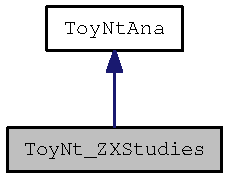
\includegraphics[width=146pt]{classToyNt__ZXStudies__inherit__graph}
\end{center}
\end{figure}
Collaboration diagram for ToyNt\_\-ZXStudies:\nopagebreak
\begin{figure}[H]
\begin{center}
\leavevmode
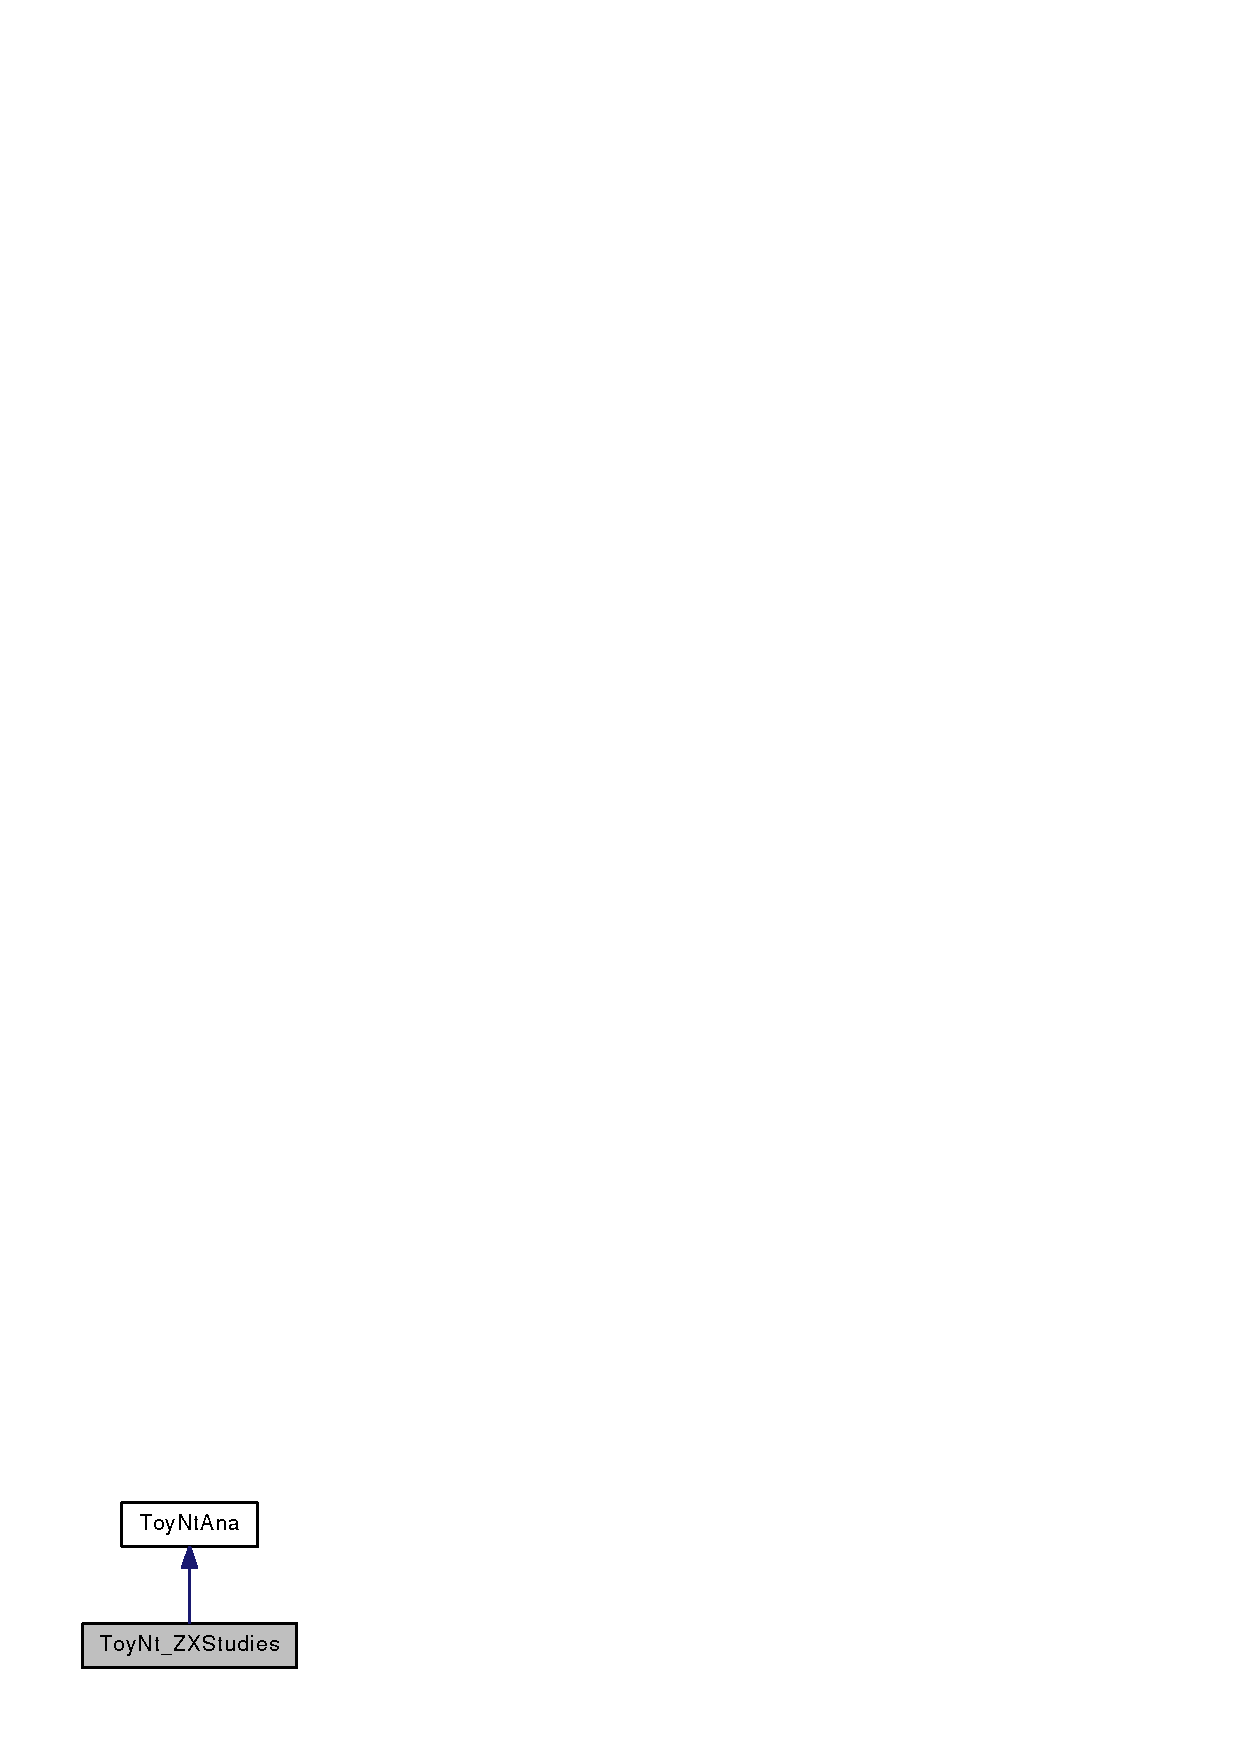
\includegraphics[width=146pt]{classToyNt__ZXStudies__coll__graph}
\end{center}
\end{figure}
\subsection*{Public Member Functions}
\begin{DoxyCompactItemize}
\item 
\hypertarget{classToyNt__ZXStudies_a8f0ccec30d23c410050699763fa95d11}{
virtual void {\bfseries Begin} (TTree $\ast$tree)}
\label{classToyNt__ZXStudies_a8f0ccec30d23c410050699763fa95d11}

\item 
\hypertarget{classToyNt__ZXStudies_abe3160b46af50772d430195bd9d63a19}{
virtual void {\bfseries Terminate} ()}
\label{classToyNt__ZXStudies_abe3160b46af50772d430195bd9d63a19}

\item 
\hypertarget{classToyNt__ZXStudies_aee258e853ab3ffd7161289a17399c9b3}{
virtual Bool\_\-t {\bfseries Process} (Long64\_\-t entry)}
\label{classToyNt__ZXStudies_aee258e853ab3ffd7161289a17399c9b3}

\item 
\hypertarget{classToyNt__ZXStudies_a3c3b86261e3a74d0ac9fa97c9f23fa2b}{
void {\bfseries Analyze} ()}
\label{classToyNt__ZXStudies_a3c3b86261e3a74d0ac9fa97c9f23fa2b}

\item 
\hypertarget{classToyNt__ZXStudies_a5ee1ac5639d64ec1304f38a6de379041}{
{\bfseries ClassDef} (\hyperlink{classToyNt__ZXStudies}{ToyNt\_\-ZXStudies}, 1)}
\label{classToyNt__ZXStudies_a5ee1ac5639d64ec1304f38a6de379041}

\end{DoxyCompactItemize}
\subsection*{Public Attributes}
\begin{DoxyCompactItemize}
\item 
\hypertarget{classToyNt__ZXStudies_ad707f0d5cfc2848f9f65fcd1168cbda1}{
ofstream {\bfseries out}}
\label{classToyNt__ZXStudies_ad707f0d5cfc2848f9f65fcd1168cbda1}

\end{DoxyCompactItemize}
\subsection*{Protected Member Functions}
\begin{DoxyCompactItemize}
\item 
\hypertarget{classToyNt__ZXStudies_ae59e95a4ce6251d4538f296d759200b0}{
void {\bfseries bookHistograms} (TDirectory $\ast$hDir)}
\label{classToyNt__ZXStudies_ae59e95a4ce6251d4538f296d759200b0}

\item 
\hypertarget{classToyNt__ZXStudies_af4bd79dcb3d639fdb220c1279d84f57b}{
void {\bfseries saveHistograms} (TDirectory $\ast$hDir)}
\label{classToyNt__ZXStudies_af4bd79dcb3d639fdb220c1279d84f57b}

\item 
\hypertarget{classToyNt__ZXStudies_a6bb336df0cc42d06617d41853d27825e}{
int {\bfseries nCentralJ} (float pTmin=25, float jvf=0.2, bool notBTag=true, bool useAbs=false)}
\label{classToyNt__ZXStudies_a6bb336df0cc42d06617d41853d27825e}

\item 
\hypertarget{classToyNt__ZXStudies_ad7faa5b2b7cfa9d57ddfa007f16dedf1}{
int {\bfseries nBJet} (float pTmin=20)}
\label{classToyNt__ZXStudies_ad7faa5b2b7cfa9d57ddfa007f16dedf1}

\item 
\hypertarget{classToyNt__ZXStudies_a533cf593e33bdf493ae89a85b782ee29}{
int {\bfseries nFwdJ} (float pTmin=30)}
\label{classToyNt__ZXStudies_a533cf593e33bdf493ae89a85b782ee29}

\end{DoxyCompactItemize}
\subsection*{Protected Attributes}
\begin{DoxyCompactItemize}
\item 
\hypertarget{classToyNt__ZXStudies_aaa6c17b5be07c3cd400a55b8d0e7c9b2}{
TGuiUtils $\ast$ {\bfseries \_\-utils}}
\label{classToyNt__ZXStudies_aaa6c17b5be07c3cd400a55b8d0e7c9b2}

\item 
\hypertarget{classToyNt__ZXStudies_a6ed68fdcd26c1aaa2731472a417d12e8}{
TH1F $\ast$ {\bfseries h\_\-pTll} \mbox{[}3\mbox{]}\mbox{[}nCUT\mbox{]}}
\label{classToyNt__ZXStudies_a6ed68fdcd26c1aaa2731472a417d12e8}

\item 
\hypertarget{classToyNt__ZXStudies_a799014534de8fe260b141ee0a06d9806}{
TH1F $\ast$ {\bfseries h\_\-met} \mbox{[}3\mbox{]}\mbox{[}nCUT\mbox{]}}
\label{classToyNt__ZXStudies_a799014534de8fe260b141ee0a06d9806}

\item 
\hypertarget{classToyNt__ZXStudies_a4441283ef9cc8b593aa36f4a15ec9e16}{
TH1F $\ast$ {\bfseries h\_\-metrel} \mbox{[}3\mbox{]}\mbox{[}nCUT\mbox{]}}
\label{classToyNt__ZXStudies_a4441283ef9cc8b593aa36f4a15ec9e16}

\item 
\hypertarget{classToyNt__ZXStudies_a038c9c8be3c7c8e6cdc9e0c55ccac7ec}{
TH1F $\ast$ {\bfseries h\_\-nJets} \mbox{[}3\mbox{]}\mbox{[}nCUT\mbox{]}}
\label{classToyNt__ZXStudies_a038c9c8be3c7c8e6cdc9e0c55ccac7ec}

\item 
\hypertarget{classToyNt__ZXStudies_af97e398e222680ba3d81bfd36fb6d10c}{
TH1F $\ast$ {\bfseries h\_\-nC20} \mbox{[}3\mbox{]}\mbox{[}nCUT\mbox{]}}
\label{classToyNt__ZXStudies_af97e398e222680ba3d81bfd36fb6d10c}

\item 
\hypertarget{classToyNt__ZXStudies_a71245217189b975fdff4eb2330aa617c}{
TH1F $\ast$ {\bfseries h\_\-nB20} \mbox{[}3\mbox{]}\mbox{[}nCUT\mbox{]}}
\label{classToyNt__ZXStudies_a71245217189b975fdff4eb2330aa617c}

\item 
\hypertarget{classToyNt__ZXStudies_a2e2b7125c7f1912b5d3cc2ae841b93f1}{
TH1F $\ast$ {\bfseries h\_\-nF30} \mbox{[}3\mbox{]}\mbox{[}nCUT\mbox{]}}
\label{classToyNt__ZXStudies_a2e2b7125c7f1912b5d3cc2ae841b93f1}

\item 
\hypertarget{classToyNt__ZXStudies_a274ebc242de22a58e0da62dc52f679a0}{
TH1F $\ast$ {\bfseries h\_\-jPt} \mbox{[}3\mbox{]}\mbox{[}nCUT\mbox{]}}
\label{classToyNt__ZXStudies_a274ebc242de22a58e0da62dc52f679a0}

\item 
\hypertarget{classToyNt__ZXStudies_a58a92268a58b209a4f899da81261908b}{
TH1F $\ast$ {\bfseries h\_\-j1Pt} \mbox{[}3\mbox{]}\mbox{[}nCUT\mbox{]}}
\label{classToyNt__ZXStudies_a58a92268a58b209a4f899da81261908b}

\end{DoxyCompactItemize}
\subsection*{Static Protected Attributes}
\begin{DoxyCompactItemize}
\item 
\hypertarget{classToyNt__ZXStudies_a001fe31fbe3a00779bee3f985ed6ec0c}{
static const int {\bfseries nCUT} = 30}
\label{classToyNt__ZXStudies_a001fe31fbe3a00779bee3f985ed6ec0c}

\end{DoxyCompactItemize}


The documentation for this class was generated from the following files:\begin{DoxyCompactItemize}
\item 
SusyWeakProdAna/ToyNt\_\-ZXStudies.h\item 
Root/ToyNt\_\-ZXStudies.cxx\end{DoxyCompactItemize}

\hypertarget{classToyNtAna}{
\section{ToyNtAna Class Reference}
\label{classToyNtAna}\index{ToyNtAna@{ToyNtAna}}
}
Inheritance diagram for ToyNtAna:\nopagebreak
\begin{figure}[H]
\begin{center}
\leavevmode
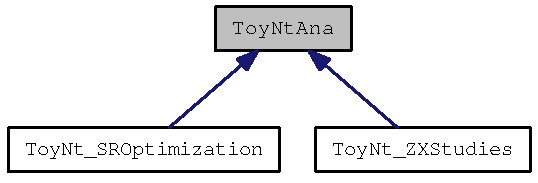
\includegraphics[width=294pt]{classToyNtAna__inherit__graph}
\end{center}
\end{figure}
\subsection*{Public Member Functions}
\begin{DoxyCompactItemize}
\item 
\hypertarget{classToyNtAna_a900d4cb959f708a25ac0df7645622752}{
{\bfseries ToyNtAna} (TTree $\ast$=0)}
\label{classToyNtAna_a900d4cb959f708a25ac0df7645622752}

\item 
\hypertarget{classToyNtAna_a955fddd314d08528d402066ee3c3612a}{
virtual Int\_\-t {\bfseries Version} () const }
\label{classToyNtAna_a955fddd314d08528d402066ee3c3612a}

\item 
\hypertarget{classToyNtAna_abbbc16db7a544ca3c1ec1ecb41e1338f}{
virtual void {\bfseries Begin} (TTree $\ast$tree)}
\label{classToyNtAna_abbbc16db7a544ca3c1ec1ecb41e1338f}

\item 
\hypertarget{classToyNtAna_a430c50c1422314d5844debf21944275d}{
virtual void {\bfseries SlaveBegin} (TTree $\ast$tree)}
\label{classToyNtAna_a430c50c1422314d5844debf21944275d}

\item 
\hypertarget{classToyNtAna_a66fa022e163ff5d31aa2451d2d6bb7b5}{
virtual void {\bfseries Init} (TTree $\ast$tree)}
\label{classToyNtAna_a66fa022e163ff5d31aa2451d2d6bb7b5}

\item 
\hypertarget{classToyNtAna_adaf14a41badd46a1ea5390ca0c244a5b}{
virtual Bool\_\-t {\bfseries Notify} ()}
\label{classToyNtAna_adaf14a41badd46a1ea5390ca0c244a5b}

\item 
\hypertarget{classToyNtAna_af717806ba276e0af9c198fdb4b50ad03}{
virtual Bool\_\-t {\bfseries Process} (Long64\_\-t entry)}
\label{classToyNtAna_af717806ba276e0af9c198fdb4b50ad03}

\item 
\hypertarget{classToyNtAna_ad6621e2f59a97b4dc9eeb84399a0cde1}{
virtual Int\_\-t {\bfseries GetEntry} (Long64\_\-t entry, Int\_\-t getall=0)}
\label{classToyNtAna_ad6621e2f59a97b4dc9eeb84399a0cde1}

\item 
\hypertarget{classToyNtAna_ac38fbeb31a4d10924d0204676c6c9108}{
virtual void {\bfseries SetOption} (const char $\ast$option)}
\label{classToyNtAna_ac38fbeb31a4d10924d0204676c6c9108}

\item 
\hypertarget{classToyNtAna_aa4f6da7849c4aedf11bf471bfb230be1}{
virtual void {\bfseries SetObject} (TObject $\ast$obj)}
\label{classToyNtAna_aa4f6da7849c4aedf11bf471bfb230be1}

\item 
\hypertarget{classToyNtAna_a258f14578de13d6ea3681f799d051758}{
virtual void {\bfseries SetInputList} (TList $\ast$input)}
\label{classToyNtAna_a258f14578de13d6ea3681f799d051758}

\item 
\hypertarget{classToyNtAna_ac48368047cf959f0915eb5e25b85e9c4}{
virtual TList $\ast$ {\bfseries GetOutputList} () const }
\label{classToyNtAna_ac48368047cf959f0915eb5e25b85e9c4}

\item 
\hypertarget{classToyNtAna_a6109af6f1ca8af3ec96c3196e0027b8e}{
virtual void {\bfseries SlaveTerminate} ()}
\label{classToyNtAna_a6109af6f1ca8af3ec96c3196e0027b8e}

\item 
\hypertarget{classToyNtAna_a77c192f64e86eddec09a9498bdd8400c}{
virtual void {\bfseries Terminate} ()}
\label{classToyNtAna_a77c192f64e86eddec09a9498bdd8400c}

\item 
\hypertarget{classToyNtAna_a8d815897ce02f3e7d3253643d130a16c}{
std::string {\bfseries sampleName} ()}
\label{classToyNtAna_a8d815897ce02f3e7d3253643d130a16c}

\item 
\hypertarget{classToyNtAna_afddaf2b07ac4043b2ed9c7029ddea935}{
void {\bfseries setSampleName} (std::string s)}
\label{classToyNtAna_afddaf2b07ac4043b2ed9c7029ddea935}

\item 
\hypertarget{classToyNtAna_a8a830a6c226f859733b397c7dc46e957}{
void {\bfseries setDebug} (int dbg)}
\label{classToyNtAna_a8a830a6c226f859733b397c7dc46e957}

\item 
\hypertarget{classToyNtAna_a7c5725725b32bf1d6fc1173d0f72ec3a}{
int {\bfseries dbg} ()}
\label{classToyNtAna_a7c5725725b32bf1d6fc1173d0f72ec3a}

\item 
\hypertarget{classToyNtAna_a502b684373b9b63abf8728eae8eb6e20}{
void {\bfseries setEvtDebug} ()}
\label{classToyNtAna_a502b684373b9b63abf8728eae8eb6e20}

\item 
\hypertarget{classToyNtAna_acda7021aad02c87fe12ad37d962d0dc0}{
bool {\bfseries dbgEvt} () const }
\label{classToyNtAna_acda7021aad02c87fe12ad37d962d0dc0}

\item 
\hypertarget{classToyNtAna_a275b66af1cdcf539b3fff1aa319cc321}{
void {\bfseries loadEventList} ()}
\label{classToyNtAna_a275b66af1cdcf539b3fff1aa319cc321}

\item 
\hypertarget{classToyNtAna_aa0569af1e91b31d900f01265723c3186}{
bool {\bfseries processThisEvent} (unsigned int run, unsigned int event)}
\label{classToyNtAna_aa0569af1e91b31d900f01265723c3186}

\item 
\hypertarget{classToyNtAna_a4e17cec76931d898cf17e496d41b2b47}{
bool {\bfseries checkRunEvent} (const RunEventMap \&runEventMap, unsigned int run, unsigned int event)}
\label{classToyNtAna_a4e17cec76931d898cf17e496d41b2b47}

\item 
\hypertarget{classToyNtAna_ab3e07647a3097c8a271eb58d87e5be0e}{
bool {\bfseries checkAndAddRunEvent} (RunEventMap \&runEventMap, unsigned int run, unsigned int event)}
\label{classToyNtAna_ab3e07647a3097c8a271eb58d87e5be0e}

\item 
\hypertarget{classToyNtAna_a4c19c8798efab68e678a6a9d21cb49a2}{
void {\bfseries addRunEvent} (RunEventMap \&runEventMap, unsigned int run, unsigned int event)}
\label{classToyNtAna_a4c19c8798efab68e678a6a9d21cb49a2}

\item 
\hypertarget{classToyNtAna_ae858d799c14279a31aae485ebd2c2e2e}{
{\bfseries ClassDef} (\hyperlink{classToyNtAna}{ToyNtAna}, 0)}
\label{classToyNtAna_ae858d799c14279a31aae485ebd2c2e2e}

\end{DoxyCompactItemize}
\subsection*{Public Attributes}
\begin{DoxyCompactItemize}
\item 
\hypertarget{classToyNtAna_a48efee8b94cd3473d15a06112283d8fc}{
TDirectory $\ast$ {\bfseries \_\-histoDir}}
\label{classToyNtAna_a48efee8b94cd3473d15a06112283d8fc}

\item 
\hypertarget{classToyNtAna_a3a86332be1a416d60d98d08a4b2bed40}{
std::string {\bfseries m\_\-sample}}
\label{classToyNtAna_a3a86332be1a416d60d98d08a4b2bed40}

\item 
\hypertarget{classToyNtAna_a4fcfcb1348348b66e9b34bbdb6a6f31b}{
TTree $\ast$ {\bfseries fChain}}
\label{classToyNtAna_a4fcfcb1348348b66e9b34bbdb6a6f31b}

\item 
\hypertarget{classToyNtAna_a6e6fd06c5edc8e6103bd10f37f6a7923}{
Long64\_\-t \hyperlink{classToyNtAna_a6e6fd06c5edc8e6103bd10f37f6a7923}{m\_\-entry}}
\label{classToyNtAna_a6e6fd06c5edc8e6103bd10f37f6a7923}

\begin{DoxyCompactList}\small\item\em pointer to the analyzed TTree or TChain \item\end{DoxyCompactList}\item 
\hypertarget{classToyNtAna_a44208eb30829347946ed7d181710f48d}{
Long64\_\-t {\bfseries m\_\-chainEntry}}
\label{classToyNtAna_a44208eb30829347946ed7d181710f48d}

\item 
\hypertarget{classToyNtAna_a0081d718751266dd0fa300a3b8308759}{
int {\bfseries m\_\-dbg}}
\label{classToyNtAna_a0081d718751266dd0fa300a3b8308759}

\item 
\hypertarget{classToyNtAna_a74045c61c388ed5ca2b622f82a1a6c1c}{
bool {\bfseries m\_\-dbgEvt}}
\label{classToyNtAna_a74045c61c388ed5ca2b622f82a1a6c1c}

\item 
\hypertarget{classToyNtAna_a1f4d3740885c1233f1675710e0e4a543}{
RunEventMap {\bfseries m\_\-eventList}}
\label{classToyNtAna_a1f4d3740885c1233f1675710e0e4a543}

\item 
\hypertarget{classToyNtAna_a116a6e87d5e483e61caa62b9a44ef447}{
RunEventMap {\bfseries m\_\-eventListDuplicate}}
\label{classToyNtAna_a116a6e87d5e483e61caa62b9a44ef447}

\item 
\hypertarget{classToyNtAna_ae4abffffa168d8cd2e95e8cdb04d724c}{
Int\_\-t {\bfseries run}}
\label{classToyNtAna_ae4abffffa168d8cd2e95e8cdb04d724c}

\item 
\hypertarget{classToyNtAna_a1cf05e1c8ffc80c18afa44485d694264}{
Int\_\-t {\bfseries event}}
\label{classToyNtAna_a1cf05e1c8ffc80c18afa44485d694264}

\item 
\hypertarget{classToyNtAna_a3953a6a1eba56e33c04fdfcf588a5093}{
Float\_\-t {\bfseries npv}}
\label{classToyNtAna_a3953a6a1eba56e33c04fdfcf588a5093}

\item 
\hypertarget{classToyNtAna_ac1bf783dae9f5a213e78c44d205250cc}{
Float\_\-t {\bfseries npvCorr}}
\label{classToyNtAna_ac1bf783dae9f5a213e78c44d205250cc}

\item 
\hypertarget{classToyNtAna_a1da0ec67b6a6464dba2febb3e417549d}{
Int\_\-t {\bfseries iSR}}
\label{classToyNtAna_a1da0ec67b6a6464dba2febb3e417549d}

\item 
\hypertarget{classToyNtAna_a54e992a33449a529fbb4ba88a6854170}{
Int\_\-t {\bfseries llType}}
\label{classToyNtAna_a54e992a33449a529fbb4ba88a6854170}

\item 
\hypertarget{classToyNtAna_a3984f5098e495d87832666f0b7dc0e78}{
Double\_\-t {\bfseries w}}
\label{classToyNtAna_a3984f5098e495d87832666f0b7dc0e78}

\item 
\hypertarget{classToyNtAna_a7c1493190370bb888a3f1927df6eea84}{
Int\_\-t {\bfseries nlep}}
\label{classToyNtAna_a7c1493190370bb888a3f1927df6eea84}

\item 
\hypertarget{classToyNtAna_ac95b5d206ff6a7c18fc672c32a89b076}{
Float\_\-t {\bfseries l\_\-pt} \mbox{[}2\mbox{]}}
\label{classToyNtAna_ac95b5d206ff6a7c18fc672c32a89b076}

\item 
\hypertarget{classToyNtAna_ac0382b16f810c47012de5a1442e8ca78}{
Float\_\-t {\bfseries l\_\-eta} \mbox{[}2\mbox{]}}
\label{classToyNtAna_ac0382b16f810c47012de5a1442e8ca78}

\item 
\hypertarget{classToyNtAna_a5cf06b9a0a6fb57d8a16f0597be397b7}{
Float\_\-t {\bfseries l\_\-phi} \mbox{[}2\mbox{]}}
\label{classToyNtAna_a5cf06b9a0a6fb57d8a16f0597be397b7}

\item 
\hypertarget{classToyNtAna_ae89d2851062bd351eb8f96004157ac34}{
Float\_\-t {\bfseries l\_\-e} \mbox{[}2\mbox{]}}
\label{classToyNtAna_ae89d2851062bd351eb8f96004157ac34}

\item 
\hypertarget{classToyNtAna_a917829909c5d119db0b69b326ea42295}{
Int\_\-t {\bfseries l\_\-q} \mbox{[}2\mbox{]}}
\label{classToyNtAna_a917829909c5d119db0b69b326ea42295}

\item 
\hypertarget{classToyNtAna_a690a309e09bd337d1d8a169ea257fc79}{
Float\_\-t {\bfseries l\_\-ptcone30} \mbox{[}2\mbox{]}}
\label{classToyNtAna_a690a309e09bd337d1d8a169ea257fc79}

\item 
\hypertarget{classToyNtAna_a9998826cce95d7254c0413e622a52b95}{
Float\_\-t {\bfseries l\_\-etcone30} \mbox{[}2\mbox{]}}
\label{classToyNtAna_a9998826cce95d7254c0413e622a52b95}

\item 
\hypertarget{classToyNtAna_a9f454db3505598674cc2144e7a719d94}{
Float\_\-t {\bfseries l\_\-etconetopo30} \mbox{[}2\mbox{]}}
\label{classToyNtAna_a9f454db3505598674cc2144e7a719d94}

\item 
\hypertarget{classToyNtAna_a457586d9143a452394b307c707aef018}{
Float\_\-t {\bfseries l\_\-d0} \mbox{[}2\mbox{]}}
\label{classToyNtAna_a457586d9143a452394b307c707aef018}

\item 
\hypertarget{classToyNtAna_a9c9c4b820e6106592f468a73bd92f221}{
Float\_\-t {\bfseries l\_\-z0} \mbox{[}2\mbox{]}}
\label{classToyNtAna_a9c9c4b820e6106592f468a73bd92f221}

\item 
\hypertarget{classToyNtAna_addd7f5ce2af7677287d7b2f20769325e}{
Bool\_\-t {\bfseries l\_\-isEle} \mbox{[}2\mbox{]}}
\label{classToyNtAna_addd7f5ce2af7677287d7b2f20769325e}

\item 
\hypertarget{classToyNtAna_ab31656c21d39566eae9cbd4b44b86320}{
Float\_\-t {\bfseries dphi\_\-metl} \mbox{[}2\mbox{]}}
\label{classToyNtAna_ab31656c21d39566eae9cbd4b44b86320}

\item 
\hypertarget{classToyNtAna_a8a0bfa3414c81ce146660082be490610}{
Float\_\-t {\bfseries mTl} \mbox{[}2\mbox{]}}
\label{classToyNtAna_a8a0bfa3414c81ce146660082be490610}

\item 
\hypertarget{classToyNtAna_a750d9a3f34f9006a8d65f678d038d86e}{
Float\_\-t {\bfseries pTll}}
\label{classToyNtAna_a750d9a3f34f9006a8d65f678d038d86e}

\item 
\hypertarget{classToyNtAna_a43f9349a0f95eb56e95ba0b6d9838b79}{
Float\_\-t {\bfseries phill}}
\label{classToyNtAna_a43f9349a0f95eb56e95ba0b6d9838b79}

\item 
\hypertarget{classToyNtAna_a1161c6817231df2e210202d2084ba1e0}{
Float\_\-t {\bfseries mll}}
\label{classToyNtAna_a1161c6817231df2e210202d2084ba1e0}

\item 
\hypertarget{classToyNtAna_ab2ad93a245c1c4431010961f312a42bd}{
Float\_\-t {\bfseries mll\_\-collApprox}}
\label{classToyNtAna_ab2ad93a245c1c4431010961f312a42bd}

\item 
\hypertarget{classToyNtAna_a0adf2c451b5f33648f6dc48d8456603d}{
Float\_\-t {\bfseries dR\_\-ll}}
\label{classToyNtAna_a0adf2c451b5f33648f6dc48d8456603d}

\item 
\hypertarget{classToyNtAna_a9207fce8edfbd042d1f24b99e6a501e5}{
Float\_\-t {\bfseries dphi\_\-ll}}
\label{classToyNtAna_a9207fce8edfbd042d1f24b99e6a501e5}

\item 
\hypertarget{classToyNtAna_a318831efbd7c52157ef8bdd41435dd80}{
Bool\_\-t {\bfseries isOS}}
\label{classToyNtAna_a318831efbd7c52157ef8bdd41435dd80}

\item 
\hypertarget{classToyNtAna_ad26cea052e9d47bb4526411376df4e1d}{
Int\_\-t {\bfseries nJets}}
\label{classToyNtAna_ad26cea052e9d47bb4526411376df4e1d}

\item 
\hypertarget{classToyNtAna_a2a9e63659989ad77c9b5b80291c2cd14}{
Int\_\-t {\bfseries nSJets}}
\label{classToyNtAna_a2a9e63659989ad77c9b5b80291c2cd14}

\item 
\hypertarget{classToyNtAna_ae7cade93ce4f5c10561910972adf479c}{
Int\_\-t {\bfseries nCJets}}
\label{classToyNtAna_ae7cade93ce4f5c10561910972adf479c}

\item 
\hypertarget{classToyNtAna_a729212760f4dcde89169db2edf1bc464}{
Int\_\-t {\bfseries nBJets}}
\label{classToyNtAna_a729212760f4dcde89169db2edf1bc464}

\item 
\hypertarget{classToyNtAna_a63d56db72b21e727000338782193150e}{
Int\_\-t {\bfseries nFJets}}
\label{classToyNtAna_a63d56db72b21e727000338782193150e}

\item 
\hypertarget{classToyNtAna_a651e784a8b9ba03d97e58ce3200d715f}{
Int\_\-t {\bfseries nOJets}}
\label{classToyNtAna_a651e784a8b9ba03d97e58ce3200d715f}

\item 
\hypertarget{classToyNtAna_a41f243a3bef4426d5fb385a73cfc6e2f}{
Bool\_\-t {\bfseries j\_\-isC20} \mbox{[}14\mbox{]}}
\label{classToyNtAna_a41f243a3bef4426d5fb385a73cfc6e2f}

\item 
\hypertarget{classToyNtAna_a55827a762efdb7d5c19a88a3afa5bc6d}{
Bool\_\-t {\bfseries j\_\-isB20} \mbox{[}14\mbox{]}}
\label{classToyNtAna_a55827a762efdb7d5c19a88a3afa5bc6d}

\item 
\hypertarget{classToyNtAna_a4096cc9fe914036d53e05049807ddf61}{
Bool\_\-t {\bfseries j\_\-isF30} \mbox{[}14\mbox{]}}
\label{classToyNtAna_a4096cc9fe914036d53e05049807ddf61}

\item 
\hypertarget{classToyNtAna_a1a31d3907e927cd83392f9f1edc42934}{
Bool\_\-t {\bfseries j\_\-isOJ} \mbox{[}14\mbox{]}}
\label{classToyNtAna_a1a31d3907e927cd83392f9f1edc42934}

\item 
\hypertarget{classToyNtAna_a4baec1455367469829026443dac39027}{
Float\_\-t {\bfseries j\_\-pt} \mbox{[}14\mbox{]}}
\label{classToyNtAna_a4baec1455367469829026443dac39027}

\item 
\hypertarget{classToyNtAna_ad18a9459f35e1ebf5882540e73868dbb}{
Float\_\-t {\bfseries j\_\-eta} \mbox{[}14\mbox{]}}
\label{classToyNtAna_ad18a9459f35e1ebf5882540e73868dbb}

\item 
\hypertarget{classToyNtAna_adfc625258bde53f80fa49a8aad4b0c8f}{
Float\_\-t {\bfseries j\_\-phi} \mbox{[}14\mbox{]}}
\label{classToyNtAna_adfc625258bde53f80fa49a8aad4b0c8f}

\item 
\hypertarget{classToyNtAna_a83ce2a01922b107fd16d346797352bb5}{
Float\_\-t {\bfseries j\_\-e} \mbox{[}14\mbox{]}}
\label{classToyNtAna_a83ce2a01922b107fd16d346797352bb5}

\item 
\hypertarget{classToyNtAna_aaf9ee7b5079d36851e13468cbd8491c0}{
Float\_\-t {\bfseries j\_\-jvf} \mbox{[}14\mbox{]}}
\label{classToyNtAna_aaf9ee7b5079d36851e13468cbd8491c0}

\item 
\hypertarget{classToyNtAna_aee010a7976e3dea80248a182cf2fb2c3}{
Float\_\-t {\bfseries j\_\-mv1} \mbox{[}14\mbox{]}}
\label{classToyNtAna_aee010a7976e3dea80248a182cf2fb2c3}

\item 
\hypertarget{classToyNtAna_ad8baad9a73727b26ca760d6888db9474}{
Bool\_\-t {\bfseries j\_\-isTruth} \mbox{[}14\mbox{]}}
\label{classToyNtAna_ad8baad9a73727b26ca760d6888db9474}

\item 
\hypertarget{classToyNtAna_aad4f0f95cc8666373f1ab0ddc9fbe28b}{
Int\_\-t {\bfseries j\_\-label} \mbox{[}14\mbox{]}}
\label{classToyNtAna_aad4f0f95cc8666373f1ab0ddc9fbe28b}

\item 
\hypertarget{classToyNtAna_aa6666326b2202367792dd0dcc180ab35}{
Bool\_\-t {\bfseries j\_\-isRecoil} \mbox{[}14\mbox{]}}
\label{classToyNtAna_aa6666326b2202367792dd0dcc180ab35}

\item 
\hypertarget{classToyNtAna_a7d47219574ed2035a9a3f3b0c262af22}{
Bool\_\-t {\bfseries j\_\-isSublead} \mbox{[}14\mbox{]}}
\label{classToyNtAna_a7d47219574ed2035a9a3f3b0c262af22}

\item 
\hypertarget{classToyNtAna_a9a700df9dd249b15b969e6fbfa92fc95}{
Float\_\-t {\bfseries met}}
\label{classToyNtAna_a9a700df9dd249b15b969e6fbfa92fc95}

\item 
\hypertarget{classToyNtAna_abcbb333fbe001b80061ff048749a246f}{
Float\_\-t {\bfseries met\_\-phi}}
\label{classToyNtAna_abcbb333fbe001b80061ff048749a246f}

\item 
\hypertarget{classToyNtAna_ac975c7e47030317550d58b27cbcc5881}{
Float\_\-t {\bfseries metrel}}
\label{classToyNtAna_ac975c7e47030317550d58b27cbcc5881}

\item 
\hypertarget{classToyNtAna_a549cad983975034882192c008a7dd77e}{
Float\_\-t {\bfseries met\_\-refEle}}
\label{classToyNtAna_a549cad983975034882192c008a7dd77e}

\item 
\hypertarget{classToyNtAna_ab3b7eaefd4c360f6d7c232898e928bad}{
Float\_\-t {\bfseries met\_\-refMuo}}
\label{classToyNtAna_ab3b7eaefd4c360f6d7c232898e928bad}

\item 
\hypertarget{classToyNtAna_a12888f57432159185936b9dc27d78f7a}{
Float\_\-t {\bfseries met\_\-refJet}}
\label{classToyNtAna_a12888f57432159185936b9dc27d78f7a}

\item 
\hypertarget{classToyNtAna_af0cbd2575a57e4f9f6cd3f61a366d749}{
Float\_\-t {\bfseries met\_\-cellout}}
\label{classToyNtAna_af0cbd2575a57e4f9f6cd3f61a366d749}

\item 
\hypertarget{classToyNtAna_a3fd481ecb31107aebabcfc737919e628}{
Float\_\-t {\bfseries mWWT}}
\label{classToyNtAna_a3fd481ecb31107aebabcfc737919e628}

\item 
\hypertarget{classToyNtAna_abe1be22c90d4fc7c99acbbad2a8b7779}{
Float\_\-t {\bfseries dphi\_\-metcl}}
\label{classToyNtAna_abe1be22c90d4fc7c99acbbad2a8b7779}

\item 
\hypertarget{classToyNtAna_adccfcc9129f81fe875c10cf0d3957662}{
Float\_\-t {\bfseries dphi\_\-metcj}}
\label{classToyNtAna_adccfcc9129f81fe875c10cf0d3957662}

\item 
\hypertarget{classToyNtAna_a4948f1f1a1ca512fc04d6fb0d338b2e2}{
Float\_\-t {\bfseries dphi\_\-metcoj}}
\label{classToyNtAna_a4948f1f1a1ca512fc04d6fb0d338b2e2}

\item 
\hypertarget{classToyNtAna_ae0b673439c1536cf1574c41a58826615}{
Float\_\-t {\bfseries dphi\_\-ll\_\-j1}}
\label{classToyNtAna_ae0b673439c1536cf1574c41a58826615}

\item 
\hypertarget{classToyNtAna_a495bae281adf247a0f2a88087adbff63}{
Float\_\-t {\bfseries dphi\_\-ll\_\-oj1}}
\label{classToyNtAna_a495bae281adf247a0f2a88087adbff63}

\item 
\hypertarget{classToyNtAna_a8196d8c67778f7608b8f24d09df44fa1}{
Float\_\-t {\bfseries dphi\_\-Zj}}
\label{classToyNtAna_a8196d8c67778f7608b8f24d09df44fa1}

\item 
\hypertarget{classToyNtAna_acce0828a53c843bb460b825852b39f3b}{
Float\_\-t {\bfseries mT2}}
\label{classToyNtAna_acce0828a53c843bb460b825852b39f3b}

\item 
\hypertarget{classToyNtAna_a5664804fd9b732c918c17a3ee7e85ea4}{
Float\_\-t {\bfseries mT2jj}}
\label{classToyNtAna_a5664804fd9b732c918c17a3ee7e85ea4}

\item 
\hypertarget{classToyNtAna_a7ce833efad8c373a1c06efeca2344bcf}{
Float\_\-t {\bfseries sphericity}}
\label{classToyNtAna_a7ce833efad8c373a1c06efeca2344bcf}

\item 
\hypertarget{classToyNtAna_afe94c616d837f89f03e86ce553f9aafd}{
Float\_\-t {\bfseries sphericityTrans}}
\label{classToyNtAna_afe94c616d837f89f03e86ce553f9aafd}

\item 
\hypertarget{classToyNtAna_abff97d19b22aab0372189ee04ea837a1}{
Float\_\-t {\bfseries llAcoplanarity}}
\label{classToyNtAna_abff97d19b22aab0372189ee04ea837a1}

\item 
\hypertarget{classToyNtAna_ad51d7f6832545731d44b8d712b8b58c8}{
Float\_\-t {\bfseries jjAcoplanarity}}
\label{classToyNtAna_ad51d7f6832545731d44b8d712b8b58c8}

\item 
\hypertarget{classToyNtAna_a02dd1c48b46b03afb4dbb0a628b85bd9}{
Bool\_\-t {\bfseries topTag}}
\label{classToyNtAna_a02dd1c48b46b03afb4dbb0a628b85bd9}

\item 
\hypertarget{classToyNtAna_a18a7aaac0dec8c64bf635fc6c7b80626}{
Float\_\-t {\bfseries mEff}}
\label{classToyNtAna_a18a7aaac0dec8c64bf635fc6c7b80626}

\item 
\hypertarget{classToyNtAna_af213307accf66ba2dca40d37081b8a71}{
Float\_\-t {\bfseries ST}}
\label{classToyNtAna_af213307accf66ba2dca40d37081b8a71}

\item 
\hypertarget{classToyNtAna_a96248b31321cb2a8646df07900cd41ff}{
Float\_\-t {\bfseries mjj}}
\label{classToyNtAna_a96248b31321cb2a8646df07900cd41ff}

\item 
\hypertarget{classToyNtAna_a95ed4099524b4309c45eb13b5385031d}{
Float\_\-t {\bfseries mct}}
\label{classToyNtAna_a95ed4099524b4309c45eb13b5385031d}

\item 
\hypertarget{classToyNtAna_af7e24811beb96ded589e7b322fbe3d7b}{
Float\_\-t {\bfseries mctPerp}}
\label{classToyNtAna_af7e24811beb96ded589e7b322fbe3d7b}

\item 
\hypertarget{classToyNtAna_a8574aec444a728a0928793c9472e558a}{
Float\_\-t {\bfseries mctPara}}
\label{classToyNtAna_a8574aec444a728a0928793c9472e558a}

\item 
\hypertarget{classToyNtAna_a119135ecd8190224432c5927d60a7aed}{
Float\_\-t {\bfseries JZBjets}}
\label{classToyNtAna_a119135ecd8190224432c5927d60a7aed}

\item 
\hypertarget{classToyNtAna_af44524849b472ff7b502d0260b9410cb}{
Float\_\-t {\bfseries JZBmet}}
\label{classToyNtAna_af44524849b472ff7b502d0260b9410cb}

\item 
\hypertarget{classToyNtAna_aa7c48feee3f50a2e5118fbb6857c572a}{
TBranch $\ast$ {\bfseries b\_\-run}}
\label{classToyNtAna_aa7c48feee3f50a2e5118fbb6857c572a}

\item 
\hypertarget{classToyNtAna_a8375b357663531b95a42e40493fcf11c}{
TBranch $\ast$ {\bfseries b\_\-event}}
\label{classToyNtAna_a8375b357663531b95a42e40493fcf11c}

\item 
\hypertarget{classToyNtAna_aac62ea67f4035cd19ec7922b40803f71}{
TBranch $\ast$ {\bfseries b\_\-npv}}
\label{classToyNtAna_aac62ea67f4035cd19ec7922b40803f71}

\item 
\hypertarget{classToyNtAna_a55346780a0ebcad62a47ac556eb7a620}{
TBranch $\ast$ {\bfseries b\_\-npvCorr}}
\label{classToyNtAna_a55346780a0ebcad62a47ac556eb7a620}

\item 
\hypertarget{classToyNtAna_aec316f3e17d1a7790f48f18db876b72e}{
TBranch $\ast$ {\bfseries b\_\-iSR}}
\label{classToyNtAna_aec316f3e17d1a7790f48f18db876b72e}

\item 
\hypertarget{classToyNtAna_a0fa33458b272ecbe5a77ce9072a0adfe}{
TBranch $\ast$ {\bfseries b\_\-llType}}
\label{classToyNtAna_a0fa33458b272ecbe5a77ce9072a0adfe}

\item 
\hypertarget{classToyNtAna_a721a2eb2c75a2bb5eeebfe1c91bfc74c}{
TBranch $\ast$ {\bfseries b\_\-w}}
\label{classToyNtAna_a721a2eb2c75a2bb5eeebfe1c91bfc74c}

\item 
\hypertarget{classToyNtAna_ab9c81bd38e5f779b009e996acb0704eb}{
TBranch $\ast$ {\bfseries b\_\-nlep}}
\label{classToyNtAna_ab9c81bd38e5f779b009e996acb0704eb}

\item 
\hypertarget{classToyNtAna_a1a108f45dd4f885e260c48ccf2b4abc1}{
TBranch $\ast$ {\bfseries b\_\-l\_\-pt}}
\label{classToyNtAna_a1a108f45dd4f885e260c48ccf2b4abc1}

\item 
\hypertarget{classToyNtAna_a9f80ae105c6cea68e543ee31820c0fd1}{
TBranch $\ast$ {\bfseries b\_\-l\_\-eta}}
\label{classToyNtAna_a9f80ae105c6cea68e543ee31820c0fd1}

\item 
\hypertarget{classToyNtAna_a2152a81440c7b67f02cabcc26bf91639}{
TBranch $\ast$ {\bfseries b\_\-l\_\-phi}}
\label{classToyNtAna_a2152a81440c7b67f02cabcc26bf91639}

\item 
\hypertarget{classToyNtAna_ada90eddd79741e4eb319aa57ad186f58}{
TBranch $\ast$ {\bfseries b\_\-l\_\-e}}
\label{classToyNtAna_ada90eddd79741e4eb319aa57ad186f58}

\item 
\hypertarget{classToyNtAna_a6e850ddc7ac8565f61c06a9910b9963e}{
TBranch $\ast$ {\bfseries b\_\-l\_\-q}}
\label{classToyNtAna_a6e850ddc7ac8565f61c06a9910b9963e}

\item 
\hypertarget{classToyNtAna_a88e9e89d059fe2b09c4c8a29bdb58302}{
TBranch $\ast$ {\bfseries b\_\-l\_\-ptcone30}}
\label{classToyNtAna_a88e9e89d059fe2b09c4c8a29bdb58302}

\item 
\hypertarget{classToyNtAna_ad8eeb46448eb3bec306c6117bae2174b}{
TBranch $\ast$ {\bfseries b\_\-l\_\-etcone30}}
\label{classToyNtAna_ad8eeb46448eb3bec306c6117bae2174b}

\item 
\hypertarget{classToyNtAna_a1cca3c6be2175b4e0a64027b310a30fa}{
TBranch $\ast$ {\bfseries b\_\-l\_\-etconetopo30}}
\label{classToyNtAna_a1cca3c6be2175b4e0a64027b310a30fa}

\item 
\hypertarget{classToyNtAna_aa9f3c8d0ace8daf323a29fc8ad825b0f}{
TBranch $\ast$ {\bfseries b\_\-l\_\-d0}}
\label{classToyNtAna_aa9f3c8d0ace8daf323a29fc8ad825b0f}

\item 
\hypertarget{classToyNtAna_aa3bf01d935dfd64037111f390e560945}{
TBranch $\ast$ {\bfseries b\_\-l\_\-z0}}
\label{classToyNtAna_aa3bf01d935dfd64037111f390e560945}

\item 
\hypertarget{classToyNtAna_a4e74aa41462f8cb10ed438ecb6a9534a}{
TBranch $\ast$ {\bfseries b\_\-l\_\-isEle}}
\label{classToyNtAna_a4e74aa41462f8cb10ed438ecb6a9534a}

\item 
\hypertarget{classToyNtAna_a17b51cc7af322dfca2bb6bc9420b40f8}{
TBranch $\ast$ {\bfseries b\_\-dphi\_\-metl}}
\label{classToyNtAna_a17b51cc7af322dfca2bb6bc9420b40f8}

\item 
\hypertarget{classToyNtAna_a0b747307468359b98caeb997fcecde65}{
TBranch $\ast$ {\bfseries b\_\-mTl}}
\label{classToyNtAna_a0b747307468359b98caeb997fcecde65}

\item 
\hypertarget{classToyNtAna_a23067a4665c3e2220dbac8db43628158}{
TBranch $\ast$ {\bfseries b\_\-pTll}}
\label{classToyNtAna_a23067a4665c3e2220dbac8db43628158}

\item 
\hypertarget{classToyNtAna_a652f632f4ce85385e54ec2deb4965a3b}{
TBranch $\ast$ {\bfseries b\_\-phill}}
\label{classToyNtAna_a652f632f4ce85385e54ec2deb4965a3b}

\item 
\hypertarget{classToyNtAna_ae8bc6e5618ca445e4c45b0b8cb079718}{
TBranch $\ast$ {\bfseries b\_\-mll}}
\label{classToyNtAna_ae8bc6e5618ca445e4c45b0b8cb079718}

\item 
\hypertarget{classToyNtAna_a59ede5ce740a148475638bd3eda407eb}{
TBranch $\ast$ {\bfseries b\_\-mll\_\-collApprox}}
\label{classToyNtAna_a59ede5ce740a148475638bd3eda407eb}

\item 
\hypertarget{classToyNtAna_ad48d6bc6a748991e1e500bc2b63ebff5}{
TBranch $\ast$ {\bfseries b\_\-dR\_\-ll}}
\label{classToyNtAna_ad48d6bc6a748991e1e500bc2b63ebff5}

\item 
\hypertarget{classToyNtAna_a56bc0d617add0ac3bebdaac67b32b590}{
TBranch $\ast$ {\bfseries b\_\-dphi\_\-ll}}
\label{classToyNtAna_a56bc0d617add0ac3bebdaac67b32b590}

\item 
\hypertarget{classToyNtAna_ae66e6096b95b6afe20b4d766a756338d}{
TBranch $\ast$ {\bfseries b\_\-isOS}}
\label{classToyNtAna_ae66e6096b95b6afe20b4d766a756338d}

\item 
\hypertarget{classToyNtAna_a9621c76cd528e84767570df348f3caee}{
TBranch $\ast$ {\bfseries b\_\-nJets}}
\label{classToyNtAna_a9621c76cd528e84767570df348f3caee}

\item 
\hypertarget{classToyNtAna_a70f808e2288adc55c2ee5f980574b086}{
TBranch $\ast$ {\bfseries b\_\-nSJets}}
\label{classToyNtAna_a70f808e2288adc55c2ee5f980574b086}

\item 
\hypertarget{classToyNtAna_a265690d385b57f10ac74df88c1fcd7de}{
TBranch $\ast$ {\bfseries b\_\-nCJets}}
\label{classToyNtAna_a265690d385b57f10ac74df88c1fcd7de}

\item 
\hypertarget{classToyNtAna_af339d464d4cd76e4f1f4a9db0fa12d2d}{
TBranch $\ast$ {\bfseries b\_\-nBJets}}
\label{classToyNtAna_af339d464d4cd76e4f1f4a9db0fa12d2d}

\item 
\hypertarget{classToyNtAna_a645f1f0cbf8ff49999c74a2a55d28bdb}{
TBranch $\ast$ {\bfseries b\_\-nFJets}}
\label{classToyNtAna_a645f1f0cbf8ff49999c74a2a55d28bdb}

\item 
\hypertarget{classToyNtAna_abfcc72e65e8aa3df221df4507a674350}{
TBranch $\ast$ {\bfseries b\_\-nOJets}}
\label{classToyNtAna_abfcc72e65e8aa3df221df4507a674350}

\item 
\hypertarget{classToyNtAna_a26bb2062e3387efc63001e5507085b20}{
TBranch $\ast$ {\bfseries b\_\-j\_\-isC20}}
\label{classToyNtAna_a26bb2062e3387efc63001e5507085b20}

\item 
\hypertarget{classToyNtAna_a20001705e18a192dbae841091d92760e}{
TBranch $\ast$ {\bfseries b\_\-j\_\-isB20}}
\label{classToyNtAna_a20001705e18a192dbae841091d92760e}

\item 
\hypertarget{classToyNtAna_a752e75c0d7a8577d9d1e801e2374739d}{
TBranch $\ast$ {\bfseries b\_\-j\_\-isF30}}
\label{classToyNtAna_a752e75c0d7a8577d9d1e801e2374739d}

\item 
\hypertarget{classToyNtAna_a74570a5d5febf7819a23c4e5168570ed}{
TBranch $\ast$ {\bfseries b\_\-j\_\-isOJ}}
\label{classToyNtAna_a74570a5d5febf7819a23c4e5168570ed}

\item 
\hypertarget{classToyNtAna_a19e1341ca483f8c890423817e155d69f}{
TBranch $\ast$ {\bfseries b\_\-j\_\-pt}}
\label{classToyNtAna_a19e1341ca483f8c890423817e155d69f}

\item 
\hypertarget{classToyNtAna_ab148b3a1b93bbf1e07788be6e0a1a77f}{
TBranch $\ast$ {\bfseries b\_\-j\_\-eta}}
\label{classToyNtAna_ab148b3a1b93bbf1e07788be6e0a1a77f}

\item 
\hypertarget{classToyNtAna_adbef0ec5874837cabe9265d764dd4a53}{
TBranch $\ast$ {\bfseries b\_\-j\_\-phi}}
\label{classToyNtAna_adbef0ec5874837cabe9265d764dd4a53}

\item 
\hypertarget{classToyNtAna_a253fdb4d4850f3533cfcf5a8dc12134e}{
TBranch $\ast$ {\bfseries b\_\-j\_\-e}}
\label{classToyNtAna_a253fdb4d4850f3533cfcf5a8dc12134e}

\item 
\hypertarget{classToyNtAna_a61e43fc66e1f320a1dbbd6c0df537a9f}{
TBranch $\ast$ {\bfseries b\_\-j\_\-jvf}}
\label{classToyNtAna_a61e43fc66e1f320a1dbbd6c0df537a9f}

\item 
\hypertarget{classToyNtAna_ac3e95c7fdb33981c19aea6aa975507d8}{
TBranch $\ast$ {\bfseries b\_\-j\_\-mv1}}
\label{classToyNtAna_ac3e95c7fdb33981c19aea6aa975507d8}

\item 
\hypertarget{classToyNtAna_a47ebb28c5bbf5dd957ac58f862d447a6}{
TBranch $\ast$ {\bfseries b\_\-j\_\-isTruth}}
\label{classToyNtAna_a47ebb28c5bbf5dd957ac58f862d447a6}

\item 
\hypertarget{classToyNtAna_ae5fcdbde2a6be7ed0ef7864dd91682ec}{
TBranch $\ast$ {\bfseries b\_\-j\_\-label}}
\label{classToyNtAna_ae5fcdbde2a6be7ed0ef7864dd91682ec}

\item 
\hypertarget{classToyNtAna_a2d8a996f2c927901574b0b2deef44cbf}{
TBranch $\ast$ {\bfseries b\_\-j\_\-isRecoil}}
\label{classToyNtAna_a2d8a996f2c927901574b0b2deef44cbf}

\item 
\hypertarget{classToyNtAna_ac0001f850eb742cac42451b6c08b2af2}{
TBranch $\ast$ {\bfseries b\_\-j\_\-isSublead}}
\label{classToyNtAna_ac0001f850eb742cac42451b6c08b2af2}

\item 
\hypertarget{classToyNtAna_a4cca9a92f0be1da603b53e4ebbaf7533}{
TBranch $\ast$ {\bfseries b\_\-met}}
\label{classToyNtAna_a4cca9a92f0be1da603b53e4ebbaf7533}

\item 
\hypertarget{classToyNtAna_a8b634a22d158647cdd47c025e96083d1}{
TBranch $\ast$ {\bfseries b\_\-met\_\-phi}}
\label{classToyNtAna_a8b634a22d158647cdd47c025e96083d1}

\item 
\hypertarget{classToyNtAna_a3f42d0ad82efe1cdb39d26c65432a7bd}{
TBranch $\ast$ {\bfseries b\_\-metrel}}
\label{classToyNtAna_a3f42d0ad82efe1cdb39d26c65432a7bd}

\item 
\hypertarget{classToyNtAna_a13d4879a83b107a5b5aef3daeb2bd556}{
TBranch $\ast$ {\bfseries b\_\-met\_\-refEle}}
\label{classToyNtAna_a13d4879a83b107a5b5aef3daeb2bd556}

\item 
\hypertarget{classToyNtAna_a36d927a2283abd54638f893a349bea08}{
TBranch $\ast$ {\bfseries b\_\-met\_\-refMuo}}
\label{classToyNtAna_a36d927a2283abd54638f893a349bea08}

\item 
\hypertarget{classToyNtAna_a77881197820837e4d6b6945c7c64875f}{
TBranch $\ast$ {\bfseries b\_\-met\_\-refJet}}
\label{classToyNtAna_a77881197820837e4d6b6945c7c64875f}

\item 
\hypertarget{classToyNtAna_acadeeb3e6b04448b4deab413039f4fd1}{
TBranch $\ast$ {\bfseries b\_\-met\_\-cellout}}
\label{classToyNtAna_acadeeb3e6b04448b4deab413039f4fd1}

\item 
\hypertarget{classToyNtAna_af6c853e63b39f05f6d438f22dfecc2af}{
TBranch $\ast$ {\bfseries b\_\-mWWT}}
\label{classToyNtAna_af6c853e63b39f05f6d438f22dfecc2af}

\item 
\hypertarget{classToyNtAna_aa0c7b3595114a643c8a8b2b88bf39104}{
TBranch $\ast$ {\bfseries b\_\-dphi\_\-metcl}}
\label{classToyNtAna_aa0c7b3595114a643c8a8b2b88bf39104}

\item 
\hypertarget{classToyNtAna_acf6067bccac91658ae4a97fae746dd44}{
TBranch $\ast$ {\bfseries b\_\-dphi\_\-metcj}}
\label{classToyNtAna_acf6067bccac91658ae4a97fae746dd44}

\item 
\hypertarget{classToyNtAna_a2956e3665beccf314046dd6a6f6b4455}{
TBranch $\ast$ {\bfseries b\_\-dphi\_\-metcoj}}
\label{classToyNtAna_a2956e3665beccf314046dd6a6f6b4455}

\item 
\hypertarget{classToyNtAna_a8065224c460d5c510e19666fa3120c8a}{
TBranch $\ast$ {\bfseries b\_\-dphi\_\-ll\_\-j1}}
\label{classToyNtAna_a8065224c460d5c510e19666fa3120c8a}

\item 
\hypertarget{classToyNtAna_a0577249f83e19364d7a8cbeaa17ef560}{
TBranch $\ast$ {\bfseries b\_\-dphi\_\-ll\_\-oj1}}
\label{classToyNtAna_a0577249f83e19364d7a8cbeaa17ef560}

\item 
\hypertarget{classToyNtAna_a65f5ce61904677b30b44a2ded5859893}{
TBranch $\ast$ {\bfseries b\_\-dphi\_\-Zj}}
\label{classToyNtAna_a65f5ce61904677b30b44a2ded5859893}

\item 
\hypertarget{classToyNtAna_a15dbf56c7df028e22219736b60483f11}{
TBranch $\ast$ {\bfseries b\_\-mT2}}
\label{classToyNtAna_a15dbf56c7df028e22219736b60483f11}

\item 
\hypertarget{classToyNtAna_a8d8b17cd7080944b2458d2b4abcaa494}{
TBranch $\ast$ {\bfseries b\_\-mT2jj}}
\label{classToyNtAna_a8d8b17cd7080944b2458d2b4abcaa494}

\item 
\hypertarget{classToyNtAna_a19615b94e91d36ce34afad4fa75f12f3}{
TBranch $\ast$ {\bfseries b\_\-sphericity}}
\label{classToyNtAna_a19615b94e91d36ce34afad4fa75f12f3}

\item 
\hypertarget{classToyNtAna_a4ce30aedf394aef2fdc95722e2b46ff7}{
TBranch $\ast$ {\bfseries b\_\-sphericityTrans}}
\label{classToyNtAna_a4ce30aedf394aef2fdc95722e2b46ff7}

\item 
\hypertarget{classToyNtAna_a0587bd98f4d4cfb9f975ac03f6a5fef1}{
TBranch $\ast$ {\bfseries b\_\-llAcoplanarity}}
\label{classToyNtAna_a0587bd98f4d4cfb9f975ac03f6a5fef1}

\item 
\hypertarget{classToyNtAna_a2339279d512639fce294600864c2634b}{
TBranch $\ast$ {\bfseries b\_\-jjAcoplanarity}}
\label{classToyNtAna_a2339279d512639fce294600864c2634b}

\item 
\hypertarget{classToyNtAna_a0ec2f3c45ba0f118ae80e94c103f6741}{
TBranch $\ast$ {\bfseries b\_\-topTag}}
\label{classToyNtAna_a0ec2f3c45ba0f118ae80e94c103f6741}

\item 
\hypertarget{classToyNtAna_ae62aacbf7df3e2e0f9e784ba6d25800e}{
TBranch $\ast$ {\bfseries b\_\-mEff}}
\label{classToyNtAna_ae62aacbf7df3e2e0f9e784ba6d25800e}

\item 
\hypertarget{classToyNtAna_ae43cd0e668eef665ddb00c0c7f94f46e}{
TBranch $\ast$ {\bfseries b\_\-ST}}
\label{classToyNtAna_ae43cd0e668eef665ddb00c0c7f94f46e}

\item 
\hypertarget{classToyNtAna_a6bc6e38ba7d778d84657cef7a7ec06d1}{
TBranch $\ast$ {\bfseries b\_\-mjj}}
\label{classToyNtAna_a6bc6e38ba7d778d84657cef7a7ec06d1}

\item 
\hypertarget{classToyNtAna_a97aac43312360e73c5e8e1d6ae486784}{
TBranch $\ast$ {\bfseries b\_\-mct}}
\label{classToyNtAna_a97aac43312360e73c5e8e1d6ae486784}

\item 
\hypertarget{classToyNtAna_aa3ce3048f27ef10d62d28fa30bf79e5a}{
TBranch $\ast$ {\bfseries b\_\-mctPerp}}
\label{classToyNtAna_aa3ce3048f27ef10d62d28fa30bf79e5a}

\item 
\hypertarget{classToyNtAna_afcc9eecf4994370395a67db53cd5cb1f}{
TBranch $\ast$ {\bfseries b\_\-mctPara}}
\label{classToyNtAna_afcc9eecf4994370395a67db53cd5cb1f}

\item 
\hypertarget{classToyNtAna_aa9a213d91840c30b216f69456eca3aa8}{
TBranch $\ast$ {\bfseries b\_\-JZBjets}}
\label{classToyNtAna_aa9a213d91840c30b216f69456eca3aa8}

\item 
\hypertarget{classToyNtAna_a6498711e97f6f244220b59bff9c738af}{
TBranch $\ast$ {\bfseries b\_\-JZBmet}}
\label{classToyNtAna_a6498711e97f6f244220b59bff9c738af}

\end{DoxyCompactItemize}


The documentation for this class was generated from the following files:\begin{DoxyCompactItemize}
\item 
SusyWeakProdAna/ToyNtAna.h\item 
Root/ToyNtAna.cxx\end{DoxyCompactItemize}

\hypertarget{classXsecUncertainty}{
\section{XsecUncertainty Class Reference}
\label{classXsecUncertainty}\index{XsecUncertainty@{XsecUncertainty}}
}


{\ttfamily \#include $<$XsecUncertainty.h$>$}\subsection*{Public Types}
\begin{DoxyCompactItemize}
\item 
enum {\bfseries McGroup} \{ \par
{\bfseries kUnknown}, 
{\bfseries kTtbar}, 
{\bfseries kSingleTop}, 
{\bfseries kTtbarW}, 
\par
{\bfseries kTtbarZ}, 
{\bfseries kWw}, 
{\bfseries kWz}, 
{\bfseries kZz}, 
\par
{\bfseries kWwjj}, 
{\bfseries kTriboson}, 
{\bfseries kZjets}, 
{\bfseries kHiggs}
 \}
\end{DoxyCompactItemize}
\subsection*{Public Member Functions}
\begin{DoxyCompactItemize}
\item 
\hypertarget{classXsecUncertainty_a0e28975a75c446f7b4c955f8aa902e0a}{
bool {\bfseries determineGroup} (const int dsid)}
\label{classXsecUncertainty_a0e28975a75c446f7b4c955f8aa902e0a}

\item 
\hypertarget{classXsecUncertainty_af521cd8cfe7bd65112460d064c9259c7}{
float {\bfseries fractionalUncertainty} () const }
\label{classXsecUncertainty_af521cd8cfe7bd65112460d064c9259c7}

\item 
\hypertarget{classXsecUncertainty_a6949891c43b8e4c854e58907a889c90d}{
McGroup {\bfseries groupFromDsid} (int dsid)}
\label{classXsecUncertainty_a6949891c43b8e4c854e58907a889c90d}

\item 
\hypertarget{classXsecUncertainty_a29d96d66897cc57bd0ae79afdc8e692a}{
std::string {\bfseries str} () const }
\label{classXsecUncertainty_a29d96d66897cc57bd0ae79afdc8e692a}

\end{DoxyCompactItemize}
\subsection*{Static Public Member Functions}
\begin{DoxyCompactItemize}
\item 
\hypertarget{classXsecUncertainty_aeb740b59fb80a84961cfdaf6774eb023}{
static std::string {\bfseries McGroup2str} (const McGroup g)}
\label{classXsecUncertainty_aeb740b59fb80a84961cfdaf6774eb023}

\end{DoxyCompactItemize}
\subsection*{Public Attributes}
\begin{DoxyCompactItemize}
\item 
\hypertarget{classXsecUncertainty_a957191d0071eca2474793757fdd2a094}{
bool {\bfseries m\_\-keepQuiet}}
\label{classXsecUncertainty_a957191d0071eca2474793757fdd2a094}

\end{DoxyCompactItemize}


\subsection{Detailed Description}
A class retrieve the xsec uncertainty described in sec.7.2 of the SS WH note.

The uncertainties are given by macro-\/groups, but when we run we only know the dsid. The dsid-\/group association is produced by the script .... A 100\% uncertainty is used for dsid for which we cannod determine the group.

\href{mailto:davide.gerbaudo@gmail.com}{\tt davide.gerbaudo@gmail.com} Mar 2014 

The documentation for this class was generated from the following files:\begin{DoxyCompactItemize}
\item 
SusyWeakProdAna/XsecUncertainty.h\item 
Root/XsecUncertainty.cxx\end{DoxyCompactItemize}

\printindex
\end{document}
